%%%%%%%%%% HAUPTDOKUMENT DER LATEX-VORLAGE DES IES %%%%%%%%%%%%%%%
%% Im wesentlichen basierend auf der Vorlage von Matthias Pospiech
%% http://www.matthiaspospiech.de/latex/vorlagen/allgemein/
%% f?r KOMA-Script 3.x
%% Erweitert und angepasst von Philipp Woock
%% Version 1.0
%% Januar 2011
%%%%%%%%%%%%%%%%%%%%%%%%%%%%%%%%%%%%%%%%%%%%%%%%%%%%%%%%%%%%%%%%%%

%% PW: Paket silence unterdr?ckt Warnungen. Schreibt die unterdr?ckten Sachen aber in eine .sil Datei
%% Silence braucht f?r save auch ein TeX \write :-(
% \usepackage[debrief, save]{silence}

%\usepackage[debrief]{silence}
%\RequirePackage[options]{silence} vor \documentclass{}
%\WarningFilter[PWfilt]{typearea}{Maybe no}
%\ActivateWarningFilters[PWfilt]

%\WarningsOff[Mathdots] 
%\WarningsOff[typearea] %Maybe no optimal type area settings!


%% PW: Ausschalten bekannter Warnungen.
\RequirePackage{silence}
\WarningFilter{typearea}{Maybe no optimal type area settings}
\WarningFilter{Mathdots}{Redefining amsmath commands}
\WarningFilter{latexfont}{Font shape}
\WarningFilter{pdfpages}{I will use a dummy}
\WarningFilter{caption}{Unused}
\WarningFilter{hyperref}{Rerun to get /PageLabels}


%% Dokumentenklasse (Koma Script) -----------------------------------------
\documentclass[%
  %draft,     % Entwurfsstadium
  final,      % fertiges Dokument
	% --- Paper Settings ---
	%%PW: A5 ist auch erlaubt, Univerlag nimmt A4 und A5.
	%%A4 wird einfach runterskaliert. A5 erfordert meistens Nacharbeit bei Skalierung von Titelblatt, TikZ-Bildern, Langen Formeln
  paper=a4,%
	%% Hochformat/Querformat
  paper=portrait, % landscape 
  pagesize=auto, % driver
  % --- Base Font Size ---
	%% Schriftgr??e
  fontsize=11pt,%  % 9 bei A5, 11 bei A4.
	% --- Koma Script Version ---
  version=last, %
 ]{scrbook} % Classes: scrartcl, scrreprt, scrbook
%\linespread{1.4} %% 1.4 f?r zwei ?bereinanderliegende inline-Math-Sachen. Man bedenke den Standard-LaTeX-Durchschuss von 1.2. Also 1.4*1.2=1.68 facher Zeilenabstand
%\usepackage{setspace}
%\setstretch{1.2}
%\recalctypearea
%% PW: Erlaubt mehr interne TeX-Register. In Ruhe lassen!
\usepackage{etex}

% Encoding der Quellcode-Dateien (sonst funktionieren Umlaute in den Quellcodedateien nicht)
%%%% Wer genau wei?, was er tut und unbedingt eine andere Codierung braucht, kann das hier umstellen!
% Fuer Linux -> utf8
% Fuer Windows, alte Linux Distributionen -> latin1
% Empfohlen latin1, da einige Pakete mit utf8 Zeichen nicht
% funktionieren, z.B: listings, soul.
%%%\usepackage[T1]{fontenc} % PW: Bringt keinen Vorteil es hier vorne vor inputenc zu haben.
%\usepackage[latin1]{inputenc} %% Falls es Probleme mit latin9 gibt auf latin1 stellen.
\usepackage[latin9]{inputenc}  %%PW: latin9 mit Eurozeichen und Ligaturen
%\usepackage[ansinew]{inputenc}
%\usepackage[utf8]{inputenc}
%\usepackage{ucs}
%\usepackage[utf8x]{inputenc}  % The simple answer is that utf8x is to be avoided if possible. It loads the ucs package, which for a long time was unmaintained (although there is now a new maintainer) and breaks various other things.


%%% Einstellungen f?r KOMA-Script
%%% Hier werden die KOMAoptions gesetzt wie z.B. R?nder, Kopfzeilen, einseitig/zweiseitig, Absatzabst?nde, Inhaltsverzeichnis usw.
%%% Alle Optionen sind im scrguide.pdf erkl?rt, die ihr in Eurem LaTeX-Distributionsverzeichnis bei den Docs findet!
%%% === Textbody ==============================================================
\KOMAoptions{%
   DIV=14,% (Size of Text Body, higher values = greater textbody)  %DIV 14 f�r A5, DIV 12 f�r A4
    %DIV=calc, % (also areaset/classic/current/default/last) 
   % -> after setting of spacing necessary!   
   BCOR=10mm% (Bindekorrektur) % 8 gibt einen Rand innen von 1,5 cm bei DIV16. Laut Frau Mehl entspricht 7 1,6 cm und sollte 1,8 bis 2,0 cm sein --> Jetzt 10.
	 %BCOR=0mm% 
}%
%%% === Headings ==============================================================
\KOMAoptions{%
   %%%% headings
	% headings=small,  % Small Font Size, thin spacing above and below
   % headings=normal, % Medium Font Size, medium spacing above and below
   headings=big, % Big Font Size, large spacing above and below
   %
   headings=noappendixprefix, % chapter in appendix as in body text
	headings=nochapterprefix,  % no prefix at chapters
   % headings=appendixprefix,   % inverse of 'noappendixprefix'
   % headings=chapterprefix,    % inverse of 'nochapterprefix'
   % headings=openany,   % Chapters start at any side
   % headings=openleft,  % Chapters start at left side
   headings=openright, % Chapters start at right side      
   %%% Add/Dont/Auto Dot behind section numbers 
   %%% (see DUDEN as reference)
    numbers=autoenddot
   % numbers=enddot
   % numbers=noenddot
   % secnumdepth=3 % depth of sections numbering (???)
}%
\setcounter{secnumdepth}{3}
%%% === Page Layout ===========================================================
\KOMAoptions{% (most options are for package typearea)
   twoside=false, % two side layout (alternating margins, standard in books)
   % twoside=false, % single side layout 
   % twoside=semi,  % two side layout (non alternating margins!)
   %
   twocolumn=false, % (true)
   %
  mpinclude=false,%      
   %
   headlines=2.1,%
	% headheight=2em,%
   headsepline=true,% %bedingt headinclude
   footsepline=false,% %bedingt footinclude
	 %headinclude=true,%
   %footinclude=true,%  %�ndert die komisch tiefen Seitenzahlen
	%Vakatseiten werden mit dem Style gesetzt
   cleardoublepage=empty %plain, headings
}%
%%% === Paragraph Separation ==================================================
\KOMAoptions{%
	 %%% The first two require the TikZ workaround
	 parskip=relative % change indentation according to fontsize (recommended)
   %parskip=absolute % do not change indentation according to fontsize
   %%% The following doesn't need the TikZ Workaround
   %parskip=false    % indentation of 1em
   % parskip=true   % parksip of 1 line - with free space in last line of 1em
   % parskip=full-  % parksip of 1 line - no adjustment
   % parskip=full+  % parksip of 1 line - with free space in last line of 1/4
   %parskip=full*  % parksip of 1 line - with free space in last line of 1/3     %% TeX Grouping Capacity Fehler wenn TikZ-Bilder kommen. Seltsam.
   % parskip=half   % parksip of 1/2 line - with free space in last line of 1em
   % parskip=half-  % parksip of 1/2 line - no adjustment
   % parskip=half+  % parksip of 1/2 line - with free space in last line of 1/3
   % parskip=half*  % parksip of 1/2 line - with free space in last line of 1em
}%
%%% === Table of Contents =====================================================
\setcounter{tocdepth}{3} % Depth of TOC Display
\KOMAoptions{%
   %%% Setting of 'Style' and 'Content' of TOC
   % toc=left, %
   toc=indented,%
   %
   toc=bib,
   % toc=nobib,
   % toc=bibnumbered,
   %
	% toc=index,%
   toc=noindex,
   %
   % toc=listof,
   toc=nolistof
   % toc=listofnumbered,
   %   
}%  
%%% === Lists of figures, tables etc. =========================================
\KOMAoptions{%
   %%% Setting of 'Style' and 'Content' of Lists 
   %%% (figures, tables etc)
	% --- General List Style ---
   listof=left, % tabular styles
   listof=indented, % hierarchical style
   % --- chapter highlighting ---
   % listof=chapterentry, % ??? Chapter starts are marked in figure/table
   % listof=chaptergapline, % New chapter starts are marked by a gap 
      		  			   	 % of a single line
	listof=chaptergapsmall, % New chapter starts are marked by a gap 
   	    					   % of a smallsingle line
   % listof=nochaptergap, % No Gap between chapters
   %
   % listof=leveldown, % lists are moved one level down ???
   % --- Appearance of Lists in TOC
   % listof=notoc, % Lists are not part of the TOC
   listof=totoc % add Lists to TOC without number
   % listof=totocnumbered, % add Lists to TOC with number
}%  
%%% === Bibliography ==========================================================
%% Setting of 'Style' and 'Content' of Bibliography
\KOMAoptions{%
	% bibliography=oldstyle,%
   bibliography=openstyle %,%
   % bibliography=nottotoc, % Bibliography is not part of the TOC
   % bibliography=totocnumbered, % add Bibliography to TOC with number
   %bibliography=totoc % add Bibliography to TOC without number  %%PW bibtopic-Problem test
}%
%%% === Index =================================================================
%% Setting of 'Style' and 'Content' of Index in TOC
\KOMAoptions{%
   index=nottotoc % index is not part of the TOC
	% index=totoc, % add index to TOC without number
}%
%%% === Titlepage =============================================================
%\KOMAoptions{%
   %%titlepage=true %
   %%titlepage=false %
%}%
%%% === Miscellaneous =========================================================
\KOMAoptions{% 	
   footnotes=multiple% nomultiple
   %open=any,%
   %open=left,%
   %open=right,%
   %chapterprefix=false,%
   %appendixprefix=false,%
   %chapteratlists=10pt,% entry
}%
\renewcommand*{\chapterpagestyle}{plain}
%%% Hier keinen Effekt, darf erst nach allen KOMAoptions und recalctypearea und areaset usw. stehen. --> Direkt vor begin document
%\setlength{\footskip}{1\baselineskip}  % Macht den Abstand zwischen Textunterkante und Seitenzahl kleiner. Standard 3.5 baselineskip

%%% LaTeX-Pr?ambel
%%% Hier werden Pakete eingebunden, Teil I
%%% Packages for LaTeX - programming
%
% Define commands that don't eat spaces.
\usepackage{xspace}
% IfThenElse
\usepackage{ifthen}
%%% Doc: ftp://tug.ctan.org/pub/tex-archive/macros/latex/contrib/oberdiek/ifpdf.sty
% command for testing for pdf-creation
\usepackage{ifpdf} %\ifpdf \else \fi

%%% Internal Commands: ----------------------------------------------
\makeatletter
%
\providecommand{\IfPackageLoaded}[2]{\@ifpackageloaded{#1}{#2}{}}
\providecommand{\IfPackageNotLoaded}[2]{\@ifpackageloaded{#1}{}{#2}}
\providecommand{\IfElsePackageLoaded}[3]{\@ifpackageloaded{#1}{#2}{#3}}
%
\newboolean{chapteravailable}%
\setboolean{chapteravailable}{false}%

\ifcsname chapter\endcsname
  \setboolean{chapteravailable}{true}%
\else
  \setboolean{chapteravailable}{false}%
\fi


\providecommand{\IfChapterDefined}[1]{\ifthenelse{\boolean{chapteravailable}}{#1}{}}%
\providecommand{\IfElseChapterDefined}[2]{\ifthenelse{\boolean{chapteravailable}}{#1}{#2}}%

\providecommand{\IfDefined}[2]{%
\ifcsname #1\endcsname
   #2 %
\else
     % do nothing
\fi
}

\providecommand{\IfElseDefined}[3]{%
\ifcsname #1\endcsname
   #2 %
\else
   #3 %
\fi
}

\providecommand{\IfElseUnDefined}[3]{%
\ifcsname #1\endcsname
   #3 %
\else
   #2 %
\fi
}


%
% Check for 'draft' mode - commands.
\newcommand{\IfNotDraft}[1]{\ifx\@draft\@undefined #1 \fi}
\newcommand{\IfNotDraftElse}[2]{\ifx\@draft\@undefined #1 \else #2 \fi}
\newcommand{\IfDraft}[1]{\ifx\@draft\@undefined \else #1 \fi}
%

% Define frontmatter, mainmatter and backmatter if not defined
\@ifundefined{prefrontmatter}{%
   \newcommand*{\prefrontmatter}{%
      %In Roemischen Buchstaben nummerieren (i, ii, iii)
      %\pagenumbering{roman}
			\hypersetup{pageanchor=false}
			\cleardoubleoddpage  %% M. Kohm sagt, das sollte man vor jedem Pagenumbering-Wechsel tun
			\pagenumbering{roman}%
			%\renewcommand*\thepage{\texorpdfstring{\arabic{page}}{prefrontP.\arabic{page}}}%
			%\renewcommand*{\theHpage}{prefront.\thepage} %statt front.\thepage ginge auch \arabic{chapter}.\thepage. Hauptsache eindeutig: http://de.authex.info/1132586-pdflatex-und-hyperref-mit-plainpages 
			% http://tex.stackexchange.com/questions/65182/cross-references-linking-to-wrong-equations-using-hyperref
			% oder auch: http://tex.stackexchange.com/questions/6098/wrong-hyper-references-after-resetting-chapter-counter
			%\renewcommand*\theHchapter{prefrontC.\arabic{chapter}}
    }
}{}
\@ifundefined{frontmatter}{%
   \newcommand*{\frontmatter}{%
      %In Roemischen Buchstaben nummerieren (i, ii, iii)
      %\pagenumbering{roman}
			\cleardoubleoddpage  %% M. Kohm sagt, das sollte man vor jedem Pagenumbering-Wechsel tun
			\pagenumbering{Roman}%
			\hypersetup{pageanchor=false}
			%\renewcommand*\thepage{\texorpdfstring{\arabic{page}}{frontP.\arabic{page}}}%
			%%\renewcommand*{\theHpage}{front.\thepage} %statt front.\thepage ginge auch \arabic{chapter}.\thepage. Hauptsache eindeutig: http://de.authex.info/1132586-pdflatex-und-hyperref-mit-plainpages 
			%% http://tex.stackexchange.com/questions/65182/cross-references-linking-to-wrong-equations-using-hyperref
			%% oder auch: http://tex.stackexchange.com/questions/6098/wrong-hyper-references-after-resetting-chapter-counter
			%\renewcommand*\theHchapter{frontC.\arabic{chapter}}
    }
}{}
\@ifundefined{mainmatter}{%
   % scrpage2 benoetigt den folgenden switch
   % wenn \mainmatter definiert ist.
   \newif\if@mainmatter\@mainmattertrue
   \newcommand*{\mainmatter}{%
      % -- Seitennummerierung auf Arabische Zahlen zuruecksetzen (1,2,3)
			\cleardoubleoddpage  %% M. Kohm sagt, das sollte man vor jedem Pagenumbering-Wechsel tun
      \pagenumbering{arabic}%
      %\setcounter{page}{1}%
			\hypersetup{pageanchor=true}
			%\renewcommand*\thepage{\texorpdfstring{\arabic{page}}{mainP.\arabic{page}}}%
			%%\renewcommand*{\theHpage}{main.\thepage}
			%\renewcommand\theHchapter{mainC.\arabic{chapter}}
			%\renewcommand{\theHequation}{\theHsection.\equationgrouping\arabic{equation}}
   }
}{}
\@ifundefined{backmatter}{%
   \newcommand*{\backmatter}{
      %In Roemischen Buchstaben nummerieren (i, ii, iii)
			\cleardoubleoddpage  %% M. Kohm sagt, das sollte man vor jedem Pagenumbering-Wechsel tun      
			%\pagenumbering{Roman}%
			%\renewcommand*\thepage{\texorpdfstring{\arabic{page}}{backP.\arabic{page}}}%
			%%\renewcommand*{\theHpage}{back.\thepage}
			%\renewcommand\theHchapter{backC.\arabic{chapter}}
   }
}{}

% Pakete speichern die spaeter geladen werden sollen
\newcommand{\LoadPackagesNow}{}
\newcommand{\LoadPackageLater}[1]{%
   \g@addto@macro{\LoadPackagesNow}{%
      \usepackage{#1}%
   }%
}

% Positionierung von Gleitumgebungen defaultm��ig auf htbp statt tbp setzen.
\renewcommand{\fps@figure}{htbp}
\renewcommand{\fps@table}{htbp}



\makeatother

%%% PW: Itemize-Spacing weniger verschwenderisch
\let\olditemize\itemize
\renewcommand{\itemize}{\olditemize\setlength{\itemsep}{-1em}} 
%%%%


\newboolean{iesenglishs}
\newboolean{useiosblogo}
\newboolean{printMuster}
\newboolean{isdissertation}


%%% ----------------------------------------------------------------

%% Es werden jeweils eines der begrenzt verf?gbaren TeX-\writes verwendet f?r
% Table of Contents
% List of figures
% List of tables
% List of listings
% List of theorems


%%%%%%%%%%%%%%%%%%
%%%%%%%%%%%%%%%% HIER EINSTELLEN, OB ENGLISCH ODER DEUTSCH USW.
%% Hier einstellen ob Englisch (true) oder Deutsch (false)
\setboolean{iesenglishs}{true}
%% Hier einstellen, ob Fraunhofer mit drin ist oder nicht
\setboolean{useiosblogo}{true}
%% Hier einstellen, ob MUSTER-Schriftzug gew?nscht ist oder nicht
\setboolean{printMuster}{false}
%% Hier einstellen, ob es sich um eine Dissertation handelt oder nicht.
%% Bewirkt Auslassung der Erkl?rung der Selbstst?ndigkeit.
\setboolean{isdissertation}{false}
%%%%%%%%%%%%%%%%
%%%%%%%%%%%%%%%%%%

%% Pr?ambel Teil II
% ------------------------------------------------------------------------
% LaTeX - Preambel  ******************************************************
% ------------------------------------------------------------------------
% von: Matthias Pospiech
% ========================================================================

% Strukturierung dieser Praeambel:
%    1.  Pakete die vor anderen geladen werden m�ssen
%        (calc, babel, xcolor, graphicx, amsmath, pst-pdf, ragged2e, ...)
%    2.  Schriften
%    3.  Mathematik (mathtools, fixmath, onlyamsmath, braket,
%        cancel, empheq, exscale, icomma, ...)
%    4.  Tabellen (booktabs, multirow, dcolumn, tabularx, ltxtable, supertabular)
%    5.  Text
%        5.1 Auszeichnungen (ulem, soul, url)
%        5.2 Fussnoten (footmisc)
%        5.3 Verweise (varioref)
%        5.4 Listen (enumitem, paralist, declist)
%    6.  Zitieren (csquotes, jurabib, natbib)
%    7.  PDF (microtype, hyperref, backref, hypcap, pdfpages
%    8.  Graphiken (float, flafter, placeins, subfig, wrapfig,
%        floatflt, picins, psfrag, sidecap, pict2e, curve2e)
%    9.  Sonstiges (makeidx, isodate, numprint, nomencl, acronym)
%    10. Verbatim (upquote, verbatim, fancyvrb, listings, examplep)
%    11. Wissenschaft (units)
%    12. Fancy Stuff
%    13. Layout
%       13.1.  Diverse Pakete und Einstellungen (multicol, ellipsis)
%       13.2.  Zeilenabstand (setspace)
%       13.3.  Seitenlayout (typearea, geometry)
%       13.4.  Farben
%       13.5.  Aussehen der URLS
%       13.6.  Kopf und Fusszeilen (scrpage2)
%       13.7.  Fussnoten
%       13.8.  Schriften (Sections )
%       13.9.  UeberSchriften (Chapter und Sections) (titlesec, indentfirst)
%       13.10. Captions (Schrift, Aussehen)
%              (caption, subfig, capt-of, mcaption, tocloft, multitoc, minitoc)
%    14.  Auszufuehrende Befehle


% ~~~~~~~~~~~~~~~~~~~~~~~~~~~~~~~~~~~~~~~~~~~~~~~~~~~~~~~~~~~~~~~~~~~~~~~~
% Einige Pakete muessen unbedingt vor allen anderen geladen werden
% ~~~~~~~~~~~~~~~~~~~~~~~~~~~~~~~~~~~~~~~~~~~~~~~~~~~~~~~~~~~~~~~~~~~~~~~~


%% PW: Macht in Zukunft "room for a new \write"
%% braucht l3kernel
%\usepackage{morewrites}

%% PW: Tip von H Oberdiek: Volle Ausgabe der Fehlermeldungen
\errorcontextlines=\maxdimen


%% PW: Tip von H. Oberdiek:
%% Z�hlerwert und \thepage auf jeder Seite protokollieren lassen
\usepackage{atbegshi}
\AtBeginShipout{\typeout{* Page \the\value{page} (\thepage)}}

%
%
%%% Doc: www.cs.brown.edu/system/software/latex/doc/calc.pdf
% Calculation with LaTeX
\usepackage{calc}


%% PW: Befehle mit mehr als einem optionalen Argument. 
\usepackage{xargs}

%%PW chapterbib. Macht nicht das, was es soll (Ein Literaturverzeichnis f�r jedes \include). Braucht wohl auch mehrere separate BibTeX-Durchl�ufe f�r jede include-Datei einmal :-(
%% Chapterbib muss laut Doku vor Babel. Doku ist im chapterbib.sty-File am Ende!!
%\usepackage{chapterbib}
%PW bibunits. Braucht extra-Durchl�ufe von BibTeX. Unkomfortabel.
%\usepackage{bibunits}

% Hat wohl das was ich brauche. Ersetzt Befehl \bibliography durch \btPrintCited. Mit backref-Option bei hyperref muss es nach hyperref geladen werden. Dort steht der Befehl nochmals!
%\usepackage[%
%verbose%
%]{bibtopic}

%%% Doc: ftp://tug.ctan.org/pub/tex-archive/macros/latex/required/babel/babel.pdf
% Languagesetting
\ifthenelse{\boolean{iesenglishs}}%
{\usepackage[english]{babel}}%
{\usepackage[ngerman]{babel}}


%% PW: Soll bei zu wenigen TeX \writes helfen. Aber einfach einbinden hilft nicht :-( Braucht selber auch ein write (auf den dann alles geleitet wird).
% \usepackage{rvwrite}



% default
%%\usepackage[
%%%	french,
%%	english,
%%%	german,
%%	ngerman,  %%%% PW: irgendwo gelesen: letzte Option gilt als Standardsprache
%%]{babel}

%%% Doc: ftp://tug.ctan.org/pub/tex-archive/macros/latex/contrib/xcolor/xcolor.pdf
% Farben
% Incompatible: Do not load when using pstricks !
\usepackage[
	table, % Load for using rowcolors command in tables
	cmyk, % CMYK Farbraum
]{xcolor}


%%% Doc: ftp://tug.ctan.org/pub/tex-archive/macros/latex/required/graphics/grfguide.pdf
% Bilder
\usepackage[%
	%final,
	%draft, % do not include images (faster)
	%pdftex, %f�r asymptote  %% sorgt f�r PDF mode expected, but DVI mode detected!!!!! Keinen Treiber ausw�hlen bei graphicx, sonst geht pstool nicht mehr!!!!!
]{graphicx}

%%% Doc: ftp://tug.ctan.org/pub/tex-archive/macros/latex/contrib/oberdiek/epstopdf.pdf
%% If an eps image is detected, epstopdf is automatically called to convert it to pdf format.
%% Requires: graphicx loaded


%% PW: Bisschen vorgezogen
%% Doc: ftp://tug.ctan.org/pub/tex-archive/macros/latex/contrib/marginnote/marginnote.pdf
% Summary description: marginnote allows margin note, where \marginpar fails
\usepackage{marginnote}

\usepackage{ifplatform}

%%%PW: Tip von H. Oberdiek
\usepackage{ltxcmds}[2010/04/26]
\makeatletter
\let\HashChar\ltx@hashchar
\makeatother

%%%PW: Tip von H. Oberdiek
%\begingroup
  %\catcode`\#=12 %
%\edef\x{\endgroup
  %\noexpand\newcommand*{\noexpand\HashChar}{#}%
%}\x

\ifpdf  %% PW: Bringt leider nix: PDF mode expected, but DVI mode detected hat nix damit zu tun
\usepackage{epstopdf}

\epstopdfDeclareGraphicsRule{.eps}{pdf}{.pdf}{%
  ps2pdf %
  -dEPSCrop %
	-dAutoRotatePages\HashChar /None %
  -dPDFSETTINGS\HashChar /prepress %
  -dCompatibilityLevel\HashChar 1.3 %
	-dEmbedAllFonts\HashChar true %
	-dSubsetFonts\HashChar true
  #1 \OutputFile
}

%%%%%%%%%%%%%%%%% Varianten, die alle nicht funktionieren... %%%%%%%%%%%%%%%%%%%%%%%%%%%%%%%%%%
%\epstopdfDeclareGraphicsRule{.eps}{pdf}{.pdf}{ps2pdf "-dEPSCrop" "-dAutoRotatePages\HashChar/None" "-dPDFSETTINGS\HashChar/prepress" "-dCompatibilityLevel\HashChar1.2" #1 \noexpand\OutputFile} % braucht oben definiertes Makro \HashChar

%\epstopdfDeclareGraphicsRule{.eps}{pdf}{.pdf}{ps2pdf -dEPSCrop -dAutoRotatePages\ltx@hashchar/None -dPDFSETTINGS\ltx@hashchar/prepress -dCompatibilityLevel\ltx@hashchar 1.3 #1 \OutputFile} %\ltx@hashchar ist aus ltxcmds (Oberdiek)

%\epstopdfDeclareGraphicsRule{.eps}{pdf}{.pdf}{ps2pdf "-dEPSCrop" "-dAutoRotatePages\ltx@hashchar/None" "-dPDFSETTINGS\ltx@hashchar/prepress" "-dCompatibilityLevel\ltx@hashchar1.3" #1 \OutputFile} %\ltx@hashchar ist aus ltxcmds (Oberdiek)

%\epstopdfDeclareGraphicsRule{.eps}{pdf}{.pdf}{ps2pdf -dPDFSETTINGS\string##/prepress -dCompatibilityLevel\string##1.3 #1 \OutputFile} 
%\epstopdfDeclareGraphicsRule{.eps}{pdf}{.pdf}{ps2pdf -dPDFSETTINGS\string#/prepress -dCompatibilityLevel\string#1.3 #1 \OutputFile} 
%\epstopdfDeclareGraphicsRule{.eps}{pdf}{.pdf}{ps2pdf -dPDFSETTINGS##/prepress -dCompatibilityLevel##1.3 #1 \OutputFile} % geht nicht

%\epstopdfDeclareGraphicsRule{.eps}{pdf}{.pdf}{ps2pdf "-dEPSCrop" "-dAutoRotatePages\string#/None" "-dPDFSETTINGS\string#/prepress" "-dCompatibilityLevel\string#1.3" #1 \noexpand\OutputFile}

%\epstopdfDeclareGraphicsRule{.eps}{pdf}{.pdf}{ps2pdf "-dEPSCrop" "-dAutoRotatePages=/None" "-dPDFSETTINGS=/prepress" "-dCompatibilityLevel=1.3" #1 \OutputFile}

%%% Problematisch wegen Mehrfachbedeutung der Raute: Latex: Makro, epstopdf: Platzhalter f�r Dateinamen, Unter DOS bei Batchfiles als Argument statt '='.
%\epstopdfsetup{program@epstopdf=epstopdf}
%\epstopdfDeclareGraphicsRule{.eps}{pdf}{.pdf}{epstopdf --gsopt=-dCompatibilityLevel=1.3 #1 \OutputFile}%  %Nur unter MikTeX mit Windows, nicht unter TeXlive
%}
%%%%%%%%%%%%%%%%%%%%%%%%%%%%%%%%%%%%%%%%%%%%%%%%%%%%%%%%%%%%%%%%%%%%%%%%%%%%%%%%%%%%%%%%%%%%%%%%%%%%%%
\fi

%%% Doc: ftp://tug.ctan.org/pub/tex-archive/macros/latex/required/amslatex/math/amsldoc.pdf
% Amsmath - Mathematik Basispaket
%
% fuer pst-pdf displaymath Modus vor pst-pdf benoetigt.
\usepackage[
   centertags, % (default) center tags vertically
   %tbtags,    % 'Top-or-bottom tags': For a split equation, place equation numbers level
               % with the last (resp. first) line, if numbers are on the right (resp. left).
   sumlimits,  %(default) Place the subscripts and superscripts of summation
               % symbols above and below
   %nosumlimits, % Always place the subscripts and superscripts of summation-type
               % symbols to the side, even in displayed equations.
   intlimits,  % Like sumlimits, but for integral symbols.
   %nointlimits, % (default) Opposite of intlimits.
   namelimits, % (default) Like sumlimits, but for certain 'operator names' such as
               % det, inf, lim, max, min, that traditionally have subscripts placed underneath
               % when they occur in a displayed equation.
   %nonamelimits, % Opposite of namelimits.
   %leqno,     % Place equation numbers on the left.
   %reqno,     % Place equation numbers on the right.
   fleqn,     % Position equations at a fixed indent from the left margin
   			  % rather than centered in the text column.
]{amsmath} %
% eqnarray nicht zusammen mit amsmath benutzen, siehe l2tabu.pdf f�r
% Hintergruende.


%%PW: Kommentare einf�gen
%% Braucht ein \write. Vielleicht eins zuviel, Asymptote braucht auch welche, es gibt ing. nur 16.
%\usepackage{comment}
%\includecomment{showcomment}
%\excludecomment{hidecomment}


%% Doc: ftp://tug.ctan.org/pub/tex-archive/graphics/pstricks/README
%% Im Beispiel auf der Homepage vor auto-pst-pdf
% load before graphicx
 %\usepackage{pstricks}  %%Funktioniert nicht zusammen mit pstool, weil pstool nur Unterst�tzung f�r psfrag bietet.
 %\usepackage{pst-plot, pst-node, pst-coil, pst-eps}


%%% Doc: http://www.ctan.org/tex-archive/macros/latex/contrib/pst-pdf/pst-pdf-DE.pdf
% Used to automatically integrate eps graphics in an pdf document using pdflatex.
% Requires ps4pdf macro !!!
% Download macro from http://www.ctan.org/tex-archive/macros/latex/contrib/pst-pdf/scripts/

%\usepackage[%
%   %active,       % Aktiviert den Extraktionsmodus (DVI-Ausgabe). Die explizite Angabe ist
%                  % normalerweise unn�tig (Standard im LATEX-Modus).
%   %inactive,     % Das Paket wird deaktiviert, Zu�tzlich werden die Pakete pstricks und
%                  % graphicx geladen
%   nopstricks,    % Das Paket pstricks wird nicht geladen.
%   %draft,        % Im pdfLATEX-Modus werden aus der Containerdatei eingef�gte Grafiken nur
%                  % als Rahmen dargestellt.
%   %final,        % Im pdfLATEX-Modus werden aus der Containerdatei eingef�gte Grafiken
%                  % vollst�ndig dargestellt (Standard).
%   %tightpage,    % Die Abmessung Grafiken in der Containerdatei entsprechen denen der
%                  % zugeh�rigen TEX-Boxen (Standard).
%   %notightpage,  % die Grafiken in der Containerdatei nehmen
%                  % mindestens die Gr��e des gesamten Blattes einnehmen.
%   %displaymath,  % Es werden zus�tzlich die mathematischen Umgebungen displaymath,
%                  % eqnarray und $$ extrahiert und im pdf-Modus als Grafik eingef�gt.
%]{pst-pdf}

%% Geht zusammen mit pstricks, aber nicht zusammen mit pstool. Also entweder auto-pst-pdf oder pstool.
%\usepackage[
%	on,
%%	crop=off,
%	crop=on,
%%	cleanup={log,aux,dvi,ps,pdf},
%]{auto-pst-pdf}
%%
% Notwendiger Bugfix f�r natbib Paket bei Benutzung von pst-pdf (Version <= v1.1o)
\IfPackageLoaded{pst-pdf}{
   \providecommand\makeindex{}
   \providecommand\makeglossary{}
}{}


% This package implements a workaround for the LaTeX bug that marginpars
% sometimes appear on the wrong margin.
%% PW: Hilft auch nicht
%\usepackage{mparhack}
% in some case this causes an error in the index together with package pdfpages
% the reason is unkown. Therefore I recommend to use the margins of marginnote


%% Doc: (inside relsize.sty )
%% ftp://tug.ctan.org/pub/tex-archive/macros/latex/contrib/misc/relsize.sty
%  Set the font size relative to the current font size
\usepackage{relsize}

%% Doc: ftp://tug.ctan.org/pub/tex-archive/macros/latex/contrib/ms/ragged2e.pdf
% Besserer Flatternsatz (Linksbuendig, statt Blocksatz)
\usepackage{ragged2e}

%%PW: Markus Kohms gridset zum registerhaltigen Satz. (Zeilen der Vorderseite matchen die Zeilen der R�ckseite wenn man es gegen das Licht h�lt)
%% Man muss h�ndisch an die Abs�tze \vskipnextgrid setzen und f�r jedes \vskipnextgrid braucht man (mehr od. weniger) einen extra-Durchlauf von pdfLaTeX :-(
%\usepackage{gridset}


% ~~~~~~~~~~~~~~~~~~~~~~~~~~~~~~~~~~~~~~~~~~~~~~~~~~~~~~~~~~~~~~~~~~~~~~~~
% Fonts Fonts Fonts
% ~~~~~~~~~~~~~~~~~~~~~~~~~~~~~~~~~~~~~~~~~~~~~~~~~~~~~~~~~~~~~~~~~~~~~~~~

\usepackage[T1]{fontenc} % T1 Schrift Encoding 
%% PW: Im Netz steht: Fontenc vor inputenc laden: "`you will allow all displayable utf8 characters to be available as input"' Siehe hier : http://tex.stackexchange.com/questions/13067/utf8x-vs-utf8-inputenc
% PW: Allerdings kompiliert es genauso, wenn fontenc erst hier kommt.

%\usepackage[LGR,OT1]{fontenc} % Schrift Encoding f�r Epigrafica

%\usepackage{textcomp}	 % Zusatzliche Symbole (Text Companion font extension)  %% PW: Fourier motzt was mit textcomp, egal ob es drau�en oder drin ist

%% Schriften werden in Fonts.tex geladen  %%PW: Wichtig: Nach fontenc!
% ~~~~~~~~~~~~~~~~~~~~~~~~~~~~~~~~~~~~~~~~~~~~~~~~~~~~~~~~~~~~~~~~~~~~~~~~
% Fonts Fonts Fonts
% ~~~~~~~~~~~~~~~~~~~~~~~~~~~~~~~~~~~~~~~~~~~~~~~~~~~~~~~~~~~~~~~~~~~~~~~~

% Alle Schriften die hier angegeben sind sehen im PDF richtig aus.
% Die LaTeX Standardschrift ist die Latin Modern (lmodern Paket).
% If Latin Modern is not available for your distribution you must install the
% package cm-super instead. Otherwise your fonts will look horrible in the PDF

% DO NOT LOAD ae Package for the font !



%% PW: NFSS-Erweiterungen wie zB condensed. Eigentlich wegen venturisadf drin.
\usepackage{nfssext-cfr}

%% PW: Initialen
\usepackage{lettrine}

%% ==== Zusammengesetzte Schriften  (Sans + Serif) =======================

%% - Latin Modern
%\usepackage{lmodern}  %%% PW: muss trotz mathpazo o.�. rein, damit nicht die ec-Schriften im pk-Format geladen werden. Die sind nicht skalierbar und verhindern, dass microtype anst�ndig l�uft.  %%Nochmal probiert und gab irgendwie doch keine Probleme mehr mit microtype

%\usepackage{kpfonts}

%%%%%%%%%%%% KPfonts mit Euler Math: Microtype: Letterspace -5
%\usepackage[sc,slantedGreek]{mathpazo}   %% PW mit smallcaps-Option wird ein anderer Font mit besserem Kerning verwendet  %%%% Nach Mathpazo ist mathrm in Palatino statt in kpfonts.
%\usepackage[mathpazo]{flexisym}  %%PW: Geh�rt zu breqn (s.u.)
%\usepackage{pxfonts} %%PW: Kompletterer Satz an Zeichen als Math Pazo

%\usepackage[%
%%light,%
%%fulloldstylenums,%
%%fulloldstyle,%
%%fullveryoldstyle,%
%nomath,% killt auch und insb. die mathbb-Variante. Sorgt aber daf�r, dass die Oldstyle-Zahlen in Euler-Mathfrak funktionieren
%%notext,%
%%nosf,%
%%nott,%
%%onlyrm,%
%%noamsmath,%
%%notextcomp,%
%%lighttext,%
%%oldstylenums,%
%%oldstyle,%
%%veryoldstyle,%
%%rmx,%
%%easyscsl,%
%%nofligatures,%
%%%%Math
%%lighttext,%
%%sfmath,%
%%sfmathbb,%
%%rmmathbb,%
%%nomathscript,%
%%mathcalasscript,%
%%classicReIm,%
%%uprightRoman,%
%%frenchstyle,%
%%oldstylenumsmath,%
%%oldstylemath,%
%%veryoldstylemath,%
%%narrowiints,%
%%partialup,% macht im Euler-Math aus partial ein hslash
%intlimits,%
%%widermath,%
%%noDcommand,%
%largesmallcaps%
%]{kpfonts}

\usepackage{libertine}  %% F�r Biolinum, Freier Optima-Klon
%\biolinum

\usepackage{fourier}  %%PW: Nach den kpfonts laden, sonst textcomp-Fehler. M�glicherweise w�rde es auch gehen, wenn man bei den kpfonts die Option notextcomp verwendet.
%\usepackage[scaled=0.85]{berasans}

%\cdwidth ist condensed bzw. \textcd

%% PW Die beiden ersten geh�ren zu venturis. Brachten aber nix, hat trotzdem nicht geklappt
%\usepackage{xkeyval}
%\usepackage{nfssext-cfr}  %% s.o. ist schon eingebunden

%\usepackage[%
%lf%  %%lining figures im Gegensatz zu osf (default) old style figures
%]{venturis}  %%Erzeugt keinen Fehler obwohl das Paket eigentlich venturisadf hei�t. Siehe venturisadf Dokumentation.

%% Hat nicht geklappt weil noch Problem mit MikTeX-Package, Aktivierung von Hand:
%0. Installation von Paket venturisadf �ber den MikTeX-Paketmanager. Automatisch gings irgendwie nicht :-(
%1. initexmf --edit-config-file updmap		%Da folgendes reinschreiben
%
%# Maps for using PS version of VenturisADF fonts
%Map yvt.map
%Map yv2.map
%Map yv1.map
%Map yv3.map
%Map yvo.map
%# end maps for VenturisADF
%
%2. initexmf --mkmaps
%3. initexmf -u


%\usepackage{pandora}  %%PW: Bitmapschrift! Kollidiert mit Microtype

%% PW: Optima clone: usepackage{urw-classico} oder usepackage{urw-classico}. Ist aber nicht direkt in LaTeX Distri wegen Lizenz

\renewcommand{\ttdefault}{lmtt}
%\renewcommand{\sfdefault}{lmss}        %%PW --- Latin Modern Sans f�r �berschriften
\renewcommand{\sfdefault}{fxb}  %fxb ist Biolinum. Keine Kursive!
%\renewcommand{\sfdefault}{yv1}  %yv1 ist venturis sans
%\renewcommand{\sfdefault}{yv3}  %yv3 ist venturis2 sans
\setkomafont{sectioning}{\normalcolor\bfseries}

%%PW: Palatino definiert mathrm und mathbf um, aber kpfonts �berschreibt es nicht.
%% Mathrm und Mathbf sollen wieder aus den kpfonts kommen, Mathsf ist wenn man nichts macht aus lmodern, wird auch auf kpfonts umdefiniert.
%\DeclareMathAlphabet{\mathrm} {OT1}{jkp}{m}{n}
%\DeclareMathAlphabet{\mathbf} {OT1}{jkp}{b}{n}
%\DeclareMathAlphabet{\mathsf} {OT1}{jkpss}{m}{n}


%\DeclareSymbolFont{AMSa}{U}{msa}{m}{n}
%\DeclareSymbolFont{AMSb}{U}{msb}{m}{n}

%\DeclareFontFamily{U}{msb}{}
%\DeclareFontShape{U}{msb}{m}{n}{ <5> <6> <7> <8> <9> gen * msbm <10> <10.95> <12> <14.4> <17.28> <20.74> <24.88> msbm10}  %aus LaTeX-Begleiter S.445. Gibt Problem: Er kann die msbm10 nicht finden, kein TFM file dazu.
%\DeclareFontShape{U}{msb}{m}{n}{msbm10}
%\DeclareSymbolFont{AMSb}{U}{msb}{m}{n}
%\SetSymbolFont{AMSb}{bold}{U}{msb}{b}{n}

%\DeclareSymbolFontAlphabet{\mathbb}{AMSb}

\DeclareSymbolFont{amscal}{OMS}{cmsy}{m}{n}
\SetSymbolFont{amscal}{bold}{OMS}{cmsy}{b}{n}

\DeclareSymbolFont{eulercal}{U}{zeus}{m}{n}
\SetSymbolFont{eulercal}{bold}{U}{zeus}{b}{n}


%%%PW: Mathcal und MathBB wieder r�ckdefinieren
\AtBeginDocument{%
  \let\mathbb\relax
	%%\DeclareMathAlphabet\amsa{U}{msa}{m}{n}
		\DeclareSymbolFont{AMSb}{U}{msb}{m}{n}
	%	\SetSymbolFont{AMSb}{bold}{U}{msb}{b}{n} %gibt kein bold bei der msb laut LaTeX-Begleiter. S.446
	%\DeclareMathAlphabet{\amsb}{U}{msb}{m}{n}  % habe das Gef�hl: Declare...Alphabet f�hrt viel fr�her zum "`too many alphabets"' Fehler
	%besser DeclareSymbolFontAlphabet laut LaTeX-Begleiter, wenn die Symbole bereits geladen sind (S.448)
	\DeclareSymbolFontAlphabet{\mathbb}{AMSb}
	%\SetMathAlphabet{\mathbb}{normal}{AMSb}
	%\SetMathAlphabet{\mathbb}{normal}{U}{msb}{m}{n}
	%\newcommand{\mathbb}{\amsb}
}
	
\AtBeginDocument{%
  %\let\mathcal\relax
	%\DeclareMathAlphabet\amscal{OMS}{cmsy}{m}{n}
	  %\SetMathAlphabet    \mathcal{normal}{OMS}{cmsy}{m}{n}
  %\DeclareMathAlphabet\mathbcal{OMS}       {cmsy}{b}{n}
	%besser DeclareSymbolFontAlphabet laut LaTeX-Begleiter, wenn die Symbole bereits geladen sind (S.448)
	\DeclareSymbolFontAlphabet{\mathcal}{amscal}  %braucht keines der 16 Register
  %\newcommand{\mathcal}{\amscal}
}
%
%
%%%%Mathscr definieren. Braucht man gar nicht, weil eucal daf�r da ist
\AtBeginDocument{%
  %\let\mathscr\relax
	%\DeclareMathAlphabet\eulercal{U}{zeus}{m}{n}
  %\DeclareMathAlphabet\mathbscr{U}       {zeus}{b}{n}
	  %\SetMathAlphabet    \mathscr{normal}{U}{zeus}{m}{n}
	\DeclareSymbolFontAlphabet{\mathscr}{eulercal}
  %\newcommand{\mathcal}{\eulercal}
}

%%Aus mathpazo
%\AtBeginDocument{%
  %\let\mathbb\relax
  %\DeclareMathAlphabet\PazoBB{U}{fplmbb}{m}{n}
  %\newcommand{\mathbb}{\PazoBB}
%}



%%%%PW: Mathcal wieder r�ckdefinieren	
%\AtBeginDocument{%
  %\let\mathcal\relax
	%\DeclareMathAlphabet\amscal{OMS}{cmsy}{m}{n}
	  %\SetMathAlphabet    \mathcal{normal}{OMS}{cmsy}{m}{n}
	%\DeclareMathAlphabet\mathbcal{OMS}       {cmsy}{b}{n}
	%%besser DeclareSymbolFontAlphabet laut LaTeX-Begleiter, wenn die Symbole bereits geladen sind (S.448)
	%%\DeclareSymbolFontAlphabet{\mathcal}{amscal}  %braucht keines der 16 Register
  %\newcommand{\mathcal}{\amscal}
%}
%%

%%%PW: Mathfrak wieder r�ckdefinieren	
%\AtBeginDocument{%
  %\let\mathcal\relax
	%\DeclareMathAlphabet\amscal{OMS}{cmsy}{m}{n}
	  %\SetMathAlphabet    \mathcal{normal}{OMS}{cmsy}{m}{n}
	%\DeclareMathAlphabet\mathbcal{OMS}       {cmsy}{b}{n}
	%%besser DeclareSymbolFontAlphabet laut LaTeX-Begleiter, wenn die Symbole bereits geladen sind (S.448)
	%%\DeclareSymbolFontAlphabet{\mathcal}{amscal}  %braucht keines der 16 Register
  %\newcommand{\mathcal}{\amscal}
%}
%%%



%%%% PW: Breites Dach-Symbol definieren. Wichtig f�r einige newcommand-Definitionen sp�ter
\DeclareMathSymbol{\widehatsym}{\mathord}{largesymbols}{"62}





% Recommanded to use with fonts: Aldus, Garamond, Melior, Sabon

%%PW: Achtung: Wenn auskommentiert kein Mathbold-Befehl!!
%\usepackage[                           %% --- EulerVM (MATH)
%   small,       %for smaller Fonts, 95% Normalgr��e
%   %euler-hat-accent  %Euler dach-Akzent
%   euler-digits % digits in euler fonts style
%]{eulervm}

%%PW: Euler Script: Gibt dann aber Fehler wegen zu vielen Mathealphabeten
%\usepackage[%
%mathscr%
%]%
%{eucal}%

\usepackage{mathdots}  %%PW: fixt Problem mit den \dots Befehlen
%\usepackage{eufrak}  %% PW: Euler Fraktur   %%knallt mit amssymb, was das gleiche macht

%%PW alternative Blackboard Mengenbuchstaben. Brauchen auch Math alphabet
%\usepackage[%
%%sans%
%]{dsfont} 

%% PW
\renewcommand*{\marginfont}{%
\scriptsize
%\color{red}
\sffamily
}
%%%%%

% PW:
\usepackage{pifont} % numbers in circles

%%PW:
%Palatino text with Euler math
%\usepackage{mathpple}


%%%%%%%%%%%%% Utopia with Fourier Math
%\usepackage{fourier}  %%Doch, geht mit Microtype. Fehler beim Unendlich-Zeichen (Ist Musik-Bindungsbogen) wenn eulervm geladen!


%\usepackage{cm-super}
%% -------------------
%
%% - Times, Helvetica, Courier (Word Standard...)
%\usepackage{mathptmx}
%\usepackage[scaled=.90]{helvet}
%\usepackage{courier}
%% -------------------
%%
%% - Palatino , Helvetica, Courier


%%%%%%%%%%%%% Palatino mit Euler Math: Microtype: Letterspace +5
%\usepackage[sc]{mathpazo}   %% PW mit smallcaps-Option wird ein anderer Font mit besserem Kerning verwendet

%\usepackage[scaled=.95]{helvet}
%\usepackage{courier}

%\usepackage{tgpagella}  %%TeX-Gyre erweiterte Version der URW Palladio
%%%%The TeX Gyre Pagella family consists of 4 text fonts: regular,
%%%%italic, bold and bold italic (qplr, qplri, qplb, qplbi).
%%% Pagella sollte durch microtype zus�tzliche Laufweite bekommen!

%\usepackage{breqn}  %%PW: Nach allen Mathe-bezogenen Paketen laden. Experimentell! Teil des MH bundles

%% -------------------
%
%% - Bera Schriften
%\usepackage{bera}
%% -------------------
%
%% - Charter, Bera Sans
%Charter besser per mathdesign-bitstream
%\usepackage{charter}\linespread{1.05}    %Probleme mit Microtype
%\usepackage{charter}
%\renewcommand{\sfdefault}{fvs}


%% ===== Serifen =========================================================

%\usepackage{mathpazo}                 %% --- Palatino
%\usepackage{charter}\linespread{1.05} %% --- Charter
%\usepackage{bookman}                  %% --- Bookman (laedt Avant Garde !!)
%\usepackage{newcent}                  %% --- New Century Schoolbook (laedt Avant Garde !!)

%\usepackage[%                         %% --- Fourier
%%   upright,     % Math fonts are upright
%%   expert,      % Only for EXPERT Fonts!
%%   oldstyle,    % Only for EXPERT Fonts!
%%   fulloldstyle % Only for EXPERT Fonts!
%]{fourier} %  %%PW:gut, au�er mathcal und mathbb
%

%% Gentium
%%\usepackage{gentium}


%% ===== Sans Serif ======================================================

%\usepackage[scaled=.95]{helvet}        %% --- Helvetica
%\usepackage{cmbright}                  %% --- CM-Bright (eigntlich eine Familie)  %% Geht nicht mit Microtype!!
%\usepackage{hfbright} ?????                  %% --- CM-Bright (eigntlich eine Familie) als Type1  %% Geht erst durch hfbright mit Microtype!!
%\usepackage{tpslifonts}                %% --- tpslifonts % Font for Slides
%\usepackage{avantgar}                  %% --- Avantgarde


%% Arev, Sans-serif
%\usepackage{arev}

%% Iwona
%\usepackage[math]{iwona}
%\usepackage{iwona}
%%%%\renewcommand{\rmdefault}{lm}
%\renewcommand{\rmdefault}{iwona}
%\renewcommand*\familydefault{\sfdefault} %% Only if the base font of the document is to be sans serif

%% TeX Gyre Heros
%\usepackage{tgheros}


%% URW Optima, braucht Schriftdateien
%\renewcommand*\sfdefault{uop}
%\renewcommand*\familydefault{\sfdefault} %% Only if the base font of the document is to be sans serif

%Klappt nicht wirklich
%\usepackage{epigrafica}


%%%% =========== Italics ================

%\usepackage{chancery}                  %% --- Zapf Chancery

%%%% =========== Typewriter =============

%\usepackage{courier}                   %% --- Courier
%\renewcommand{\ttdefault}{cmtl}        %% --- CmBright Typewriter Font

%\renewcommand{\ttdefault}{lmtt}        %% --- Latin Modern Typewriter Font   %%PW: Hat Probleme bei Codelistings, bfseries sieht man nicht.
%\renewcommand{\ttdefault}{txtt}        %% --- Aus txfonts (Times-Paket)   %%ist auch ganz ok, aber nahe an den kpfonts
%\usepackage{inconsolata}   %%PW: Kann kein bfseries.

%%\usepackage[scaled]{beramono}

%\usepackage[%                          %% --- Luxi Mono (Typewriter)
%   scaled=0.9%
%]{luximono}

%%\usepackage{inconsolata}  %% nicht fett und nicht kursiv!



%%%% =========== Mathe ================


%%%\renewcommand{\rmdefault}{ugm} %nicht n�tig PW. Urw GaraMond
%
%\usepackage[
%% %   adobe-utopia,
%%   garamond,
%   bitstream-charter   %% so wird Charter geladen!  %%Problem mit Unendlich-Zeichen, wenn eulervm geladen
% ]{mathdesign}


%\renewcommand{\rmdefault}{bch}		%%PW bitstream charter

%%%\renewcommand{\sfdefault}{lmss}   %%PW latin modern sans serif

%%%% (((( !!! kommerzielle Schriften !!! )))))))))))))))))))))))))))))))))))))))))))))))))))

%% ===== Serifen (kommerzielle Schriften ) ================================

%% --- Adobe Aldus
%\renewcommand{\rmdefault}{pasx}
%\renewcommand{\rmdefault}{pasj} %%oldstyle digits
% math recommended: \usepackage[small]{eulervm}

%% --- Adobe Garamond
%\usepackage[%
%   osf,        % oldstyle digits
%   scaled=1.05 %appropriate in many cases
%]{xagaramon}
% math recommended: \usepackage{eulervm}

%% --- Adobe Stempel Garamond
%\renewcommand{\rmdefault}{pegx}
%\renewcommand{\rmdefault}{pegj} %%oldstyle digits

%% --- Adobe Melior
%\renewcommand{\rmdefault}{pml}
% math recommended: %\usepackage{eulervm}

%% --- Adobe Minion
%\renewcommand{\rmdefault}{pmnx}
%\renewcommand{\rmdefault}{pmnj} %oldstyle digits
% math recommended: \usepackage[small]{eulervm} or \usepackage{mathpmnt} % commercial

%% --- Adobe Sabon
%\renewcommand{\rmdefault}{psbx}
%\renewcommand{\rmdefault}{psbj} %oldstyle digits
% math recommended: \usepackage{eulervm}

%% --- Adobe Times
% math recommended: \usepackage{mathptmx} % load first !
%\renewcommand{\rmdefault}{ptmx}
%\renewcommand{\rmdefault}{ptmj} %oldstyle digits

%% --- Linotype ITC Charter
%\renewcommand{\rmdefault}{lch}

%% --- Linotype Meridien
%\renewcommand{\rmdefault}{lmd}

%%% ===== Sans Serif (kommerzielle Schriften) ============================

%% --- Adobe Frutiger
%\usepackage[
%   scaled=0.90
%]{frutiger}

%% --- Adobe Futura (=Linotype FuturaLT) : Sans Serif
%\usepackage[
%   scaled=0.94  % appropriate in many cases
%]{futura}

%% --- Adobe Gill Sans : Sans Serif
%\usepackage{gillsans}

%% -- Adobe Myriad  : Sans Serif
%\renewcommand{\sfdefault}{pmy}
%\renewcommand{\sfdefault}{pmyc} %% condensed Font

%% --- Syntax : sans serif font
%\usepackage[
%   scaled
%]{asyntax}

%% --- Adobe Optima : Semi Sans Serif
%\usepackage[
%   medium %darker medium weight fonts
%]{optima}

%% --- Linotype ITC Officina Sans
%\renewcommand{\sfdefault}{lo9}





% ~~~~~~~~~~~~~~~~~~~~~~~~~~~~~~~~~~~~~~~~~~~~~~~~~~~~~~~~~~~~~~~~~~~~~~~~
% Math Packages
% ~~~~~~~~~~~~~~~~~~~~~~~~~~~~~~~~~~~~~~~~~~~~~~~~~~~~~~~~~~~~~~~~~~~~~~~~

% *** Mathematik **************************************
%
% amsmath schon vorher geladen da es vor pst-pdf geladen werden muss


%%% Doc: ftp://tug.ctan.org/pub/tex-archive/macros/latex/contrib/mh/doc/mathtools.pdf
% Erweitert amsmath und behebt einige Bugs.
% Muss vor ntheorem geladen werden!
\usepackage[fixamsmath,disallowspaces]{mathtools}

%%% Doc: http://www.ctan.org/info?id=fixmath
% LaTeX's default style of typesetting mathematics does not comply
% with the International Standards ISO31-0:1992 to ISO31-13:1992
% which indicate that uppercase Greek letters always be typset
% upright, as opposed to italic (even though they usually
% represent variables) and allow for typsetting of variables in a
% boldface italic style (even though the required fonts are
% available). This package ensures that uppercase Greek be typeset
% in italic style, that upright $\Delta$ and $\Omega$ symbols are
% available through the commands \upDelta and \upOmega; and
% provides a new math alphabet \mathbold for boldface
% italic letters, including Greek.

%\usepackage{fixmath}
%%%%%PW: fixmath ist schuld, dass mathbold mit eulervm nicht mehr funktioniert

%%PW:
% Ohne (!) bm-Paket gehen Formeln in �berschriften nicht mehr --> too many math alphabets used in version normal
\newcommand\hmmax{0}
\newcommand\bmmax{1}  %%2 ist schon zuviel
\usepackage{bm}
% bm an sich gibt aber auch schnell "too many math alphabets" Fehler. Insg. kann TeX 16 Mathe-Alphabete
%% Kann man wegbekommen, indem man die heavy families reduziert (hmmax) und die bold families (bmmax)
%% http://www.tex.ac.uk/cgi-bin/texfaq2html?label=manymathalph
%\renewcommand{\hmmax}{0}
%\renewcommand{\bmmax}{3}
%Boldmath mit \bm Befehl. Empfohlen im LaTeX-Begleiter. Laden nach allen Pakten, die Mathefont-Einstellungen machen.


%%% Doc: ftp://tug.ctan.org/pub/tex-archive/macros/latex/contrib/onlyamsmath/onlyamsmath.dvi
% Warnt bei Benutzung von Befehlen die mit amsmath inkompatibel sind.
\usepackage[
	all,
	warning
]{onlyamsmath}


%% PW: Asymptote Unterst�tzung. Asymptote braucht auch ein TeX-\write von denen es nur 16 gibt. Bin schon am Limit, deswegen Asymptote XOR comment (braucht auch eins).
%\usepackage[inline]{asymptote}  %%gibts erst nach Installation von Hand
%\usepackage[% %%geh�rt zu MikTeX, macht aber nicht das, was man sich erhofft.
%process=all,%
%%process=none,
%]{asyfig}

%------------------------------------------------------

% -- Vektor fett darstellen -----------------
% \let\oldvec\vec
% \def\vec#1{{\boldsymbol{#1}}} %Fetter Vektor
% \newcommand{\ve}{\vec} %
% -------------------------------------------


%%% Doc: ftp://tug.ctan.org/pub/tex-archive/macros/latex/contrib/misc/braket.sty
%\usepackage{braket}  % Quantenmechanik Bracket Schreibweise

%%% Doc: ftp://tug.ctan.org/pub/tex-archive/macros/latex/contrib/misc/cancel.sty
\usepackage{cancel}  % Durchstreichen

%%% Doc: ftp://tug.ctan.org/pub/tex-archive/macros/latex/contrib/mh/doc/empheq.pdf
\usepackage{empheq}  % Hervorheben

%%% Doc: ftp://tug.ctan.org/pub/tex-archive/info/math/voss/mathmode/Mathmode.pdf
%\usepackage{exscale} % Skaliert Mathe-Modus Ausgaben in allen Umgebungen richtig.

%%% Doc: ftp://tug.ctan.org/pub/tex-archive/macros/latex/contrib/was/icomma.dtx
% Erlaubt die Benutzung von Kommas im Mathematikmodus
\usepackage{icomma}


%%PW stackrel
\usepackage{stackrel} %provides enhanced \stackrel and \stackbin
%\stackrel [subscript] {superscript} {rel}
%\stackbin [subscript] {superscript} {bin}
%Example:
%A \stackbin[\text{and}]{}{+} B \stackrel[x]{!}{=} C

%%% Doc: http://www.ctex.org/documents/packages/special/units.pdf
\usepackage[nice]{nicefrac}

%%PW commath
%commath -- A LaTeX class which provides some commands which help you to format formulas flexibly.
%Differentiale aufrecht setzen mit vorgefertigten Operatoren, Intervalle, Senkrechter Evaluationsstrich, Norm
%%% PW: Gibt aber leider Probleme mit figureref-Befehl und wenn das drau�en ist mit "`too many math alphabets"'
%\usepackage{commath}


%%% Tauschen von Epsilon und andere:
% \let\ORGvarrho=\varrho
% \let\varrho=\rho
% \let\rho=\ORGvarrho
%
\let\ORGvarepsilon=\varepsilon
\let\varepsilon=\epsilon
\let\epsilon=\ORGvarepsilon
%
% \let\ORGvartheta=\vartheta
% \let\vartheta=\theta
% \let\theta=\ORGvartheta
%
% \let\ORGvarphi=\varphi
% \let\varphi=\phi
% \let\phi=\ORGvarphi

% Vier Indizes an beliebigen Zeichen (2 links, 2 rechts)
\usepackage{fouridx}

% Matrizen mit Randbeschriftung
\usepackage{blkarray}

%%PW: F�r Beispiele, S�tze, Lemmata: ntheorem
%%PW: amsthm gibt es auch noch, ist aber �lter
% Muss nach mathtools geladen werden!
\usepackage[amsmath,thmmarks,standard,hyperref]{ntheorem}   %hyperref-Option macht Probleme  %im Minimaltest aber nicht
%\usepackage{thmtools}   %Fuer \listoftheorems  %Nicht in MikTeX 2.8 %Wird nicht benutzt
\usepackage{theoremref}  %F�r bessere Referenzierung

% ~~~~~~~~~~~~~~~~~~~~~~~~~~~~~~~~~~~~~~~~~~~~~~~~~~~~~~~~~~~~~~~~~~~~~~~~
% Symbole
% ~~~~~~~~~~~~~~~~~~~~~~~~~~~~~~~~~~~~~~~~~~~~~~~~~~~~~~~~~~~~~~~~~~~~~~~~
%
%%% General Doc: http://www.ctan.org/tex-archive/info/symbols/comprehensive/symbols-a4.pdf
%
%% Symbole f�r Mathematiksatz
%\usepackage{mathrsfs} %% Schreibschriftbuchstaben f�r den Mathematiksatz (nur Gro�buchstaben)   %%%%% PW: Auch einfach mal reingemacht
\usepackage{dsfont}   %% Double Stroke Fonts   %%%% PW: F�r Mengensymbole R Q Z N
%\usepackage[mathcal]{euscript} %% adds euler mathcal font    %%%% PW: Mathcal ist zwar bei Eulervm schon irgendwie drin. Ist zuviel. Gibt dann "`too many math alphabets"' Fehler.
\usepackage{amssymb}      %%%% knallt mit eufrak, was das gleiche macht
%\usepackage[Symbolsmallscale]{upgreek} % upright symbols from euler package [Euler] or Adobe Symbols [Symbol]
%\usepackage[upmu]{gensymb}             % Option upmu  %% bekomme Fehler: command \upmu is undefined

%% Allgemeine Symbole
\usepackage{wasysym}  %% Doc: http://www.ctan.org/tex-archive/macros/latex/contrib/wasysym/wasysym.pdf
\usepackage{marvosym} %% Symbole aus der marvosym Schrift
\usepackage{pifont}   %% ZapfDingbats


% ~~~~~~~~~~~~~~~~~~~~~~~~~~~~~~~~~~~~~~~~~~~~~~~~~~~~~~~~~~~~~~~~~~~~~~~~
% Tables (Tabular)
% ~~~~~~~~~~~~~~~~~~~~~~~~~~~~~~~~~~~~~~~~~~~~~~~~~~~~~~~~~~~~~~~~~~~~~~~~

% Basispaket fuer alle Tabellenfunktionen
% -> wird automatisch durch andere Pakete geladen
% \usepackage{array}
%
% bessere Abstaende innerhalb der Tabelle (Layout))
% -------------------------------------------------
%%% Doc: ftp://tug.ctan.org/pub/tex-archive/macros/latex/contrib/booktabs/booktabs.pdf
\usepackage{booktabs}
%
% Farbige Tabellen
% ----------------
% Das Paket colortbl wird inzwischen automatisch durch xcolor geladen
%
% Erweiterte Funktionen innerhalb von Tabellen
% --------------------------------------------
%%% Doc: ftp://tug.ctan.org/pub/tex-archive/macros/latex/contrib/multirow/multirow.sty
\usepackage{multirow} % Mehrfachspalten
%
%%% Doc: Documentation inside dtx Package
\usepackage{dcolumn}  % Ausrichtung an Komma oder Punkt

\usepackage{tabulary}

%%% Neue Tabellen-Umgebungen:
% ---------------------------
% Spalten automatischer Breite:
%%% Doc: Documentation inside dtx Package
% \usepackage{tabularx}
% -> nach hyperref Laden
% -> wird von ltxtable geladen
% \LoadPackageLater{tabularx}


% Tabellen ueber mehere Seiten
% ----------------------------
%%% Doc: ftp://tug.ctan.org/pub/tex-archive/macros/latex/contrib/carlisle/ltxtable.pdf
% \usepackage{ltxtable} % Longtable + tabularx
                        % (multi-page tables) + (auto-sized columns in a fixed width table)
% -> nach hyperref laden
\LoadPackageLater{ltxtable}


%%% Doc: ftp://tug.ctan.org/pub/tex-archive/macros/latex/contrib/supertabular/supertabular.pdf
%\usepackage{supertabular}


% ~~~~~~~~~~~~~~~~~~~~~~~~~~~~~~~~~~~~~~~~~~~~~~~~~~~~~~~~~~~~~~~~~~~~~~~~
% text related packages
% ~~~~~~~~~~~~~~~~~~~~~~~~~~~~~~~~~~~~~~~~~~~~~~~~~~~~~~~~~~~~~~~~~~~~~~~~

%%% Textverzierungen/Auszeichnungen ======================================
%
%%% Doc: ftp://tug.ctan.org/pub/tex-archive/macros/latex/contrib/misc/ulem.sty
\usepackage[normalem]{ulem}      % Zum Unterstreichen
%%% Doc: ftp://tug.ctan.org/pub/tex-archive/macros/latex/contrib/soul/soul.pdf
\usepackage{soul}		            % Unterstreichen, Sperren
%%% Doc: ftp://tug.ctan.org/pub/tex-archive/macros/latex/contrib/misc/url.sty
\usepackage{url} % Setzen von URLs. In Verbindung mit hyperref sind diese auch aktive Links.

%%PW:  Textpos Erlaubt absolute Positionierung. F�r Titelseite.
%%%%Beispiel:
%%%%\begin{textblock}{8}(10.8,0.2)
%%%%\includegraphics[width=8cm]{bild}
%%%%\end{textblock}
%%%%Dazu muss \usepackage[absolute]{textpos} eingebunden werden.
%%%%Die erste Zahl gibt die Breite des Textblocks an (wird f�r Bilder NICHT!!! ignoriert, legt die Bildbreite fest), die
%%%%zweite den Abstand zum linken und die dritte den Abstand zum oberen Seitenrand.
\usepackage[%
absolute,%
%showboxes,%   %Hilft gewaltig beim Verst�ndnis!
%overlay,%
verbose,
]{textpos}  %% Definiert \begin{textblock}{hsize}(hpos,vpos)
\setlength{\TPHorizModule}{10mm}
\setlength{\TPVertModule}{\TPHorizModule}
\textblockorigin{0mm}{0mm} % start everything near the top-left corner

%\usepackage{eso-pic}  %% absolute Bildpositionierung


%%% Fussnoten/Endnoten ===================================================
%
%%% Doc: ftp://tug.ctan.org/pub/tex-archive/macros/latex/contrib/footmisc/footmisc.pdf
%
\usepackage[
   bottom,      % Footnotes appear always on bottom. This is necessary
                % especially when floats are used
   stable,      % Make footnotes stable in section titles
   perpage,     % Reset on each page
   %para,       % Place footnotes side by side of in one paragraph.
   %side,       % Place footnotes in the margin
   ragged,      % Use RaggedRight
   %norule,     % suppress rule above footnotes
   multiple,    % rearrange multiple footnotes intelligent in the text.
   %symbol,     % use symbols instead of numbers
]{footmisc}

\renewcommand*{\multfootsep}{,\nobreakspace}

\deffootnote%
   [1em]% width of marker
   {1.5em}% indentation (general)
   {1em}% indentation (par)
   {\textsubscript{\thefootnotemark}}%


%% Einruecken der Fussnote einstellen
%\setlength\footnotemargin{10pt}

%--- footnote counter documentweit durchlaufend ------------------------------
%\usepackage{chngcntr}
%\counterwithout{footnote}{chapter}
%-----------------------------------------------------------------------------

%%% Doc: ftp://tug.ctan.org/pub/tex-archive/macros/latex/contrib/misc/endnotes.sty
%\usepackage{endnotes}
% From the Documentation:
% To turn all the footnotes in your documents into endnotes, say
%
%     \let\footnote=\endnote
%
%  in your preamble, and then add something like
%
%     \newpage
%     \begingroup
%     \parindent 0pt
%     \parskip 2ex
%     \def\enotesize{\normalsize}
%     \theendnotes
%     \endgroup
%
% as the last thing in your document.  (But \theendnotes all
% by itself will work.)

%%% Verweise =============================================================
%
%%% Doc: Documentation inside dtx File
\usepackage[ngerman]{varioref} % Intelligente Querverweise

%%% Listen ===============================================================
%
%
%%% Doc: ftp://tug.ctan.org/pub/tex-archive/macros/latex/contrib/paralist/paralist.pdf
% \usepackage{paralist}
%
%%% Doc: ftp://tug.ctan.org/pub/tex-archive/macros/latex/contrib/enumitem/enumitem.pdf
% Better than 'paralist' and 'enumerate' because it uses a keyvalue interface !
% Do not load together with enumerate.
\IfPackageNotLoaded{enumerate}{
	\usepackage{enumitem}
}
%
%%% Doc: ftp://tug.ctan.org/pub/tex-archive/macros/latex/contrib/ncctools/doc/desclist.pdf
% Improved description environment
%\usepackage{declist}


\usepackage{blindtext}   %PW: Lorem ipsum deutsch.

% ~~~~~~~~~~~~~~~~~~~~~~~~~~~~~~~~~~~~~~~~~~~~~~~~~~~~~~~~~~~~~~~~~~~~~~~~
% Pakete zum Zitieren
% ~~~~~~~~~~~~~~~~~~~~~~~~~~~~~~~~~~~~~~~~~~~~~~~~~~~~~~~~~~~~~~~~~~~~~~~~

% Quotes =================================================================
%% Doc: ftp://tug.ctan.org/pub/tex-archive/macros/latex/contrib/csquotes/csquotes.pdf
%%% Advanced features for clever quotations
%\usepackage[%
   %autostyle=true,% the style of all quotation marks will be adapted
                     %%% to the document language as chosen by 'babel' or polyglossia. Option babel is deprecated
   %%%german=quotes,		% Styles of quotes in each language
   %german=guillemets%,		% Styles of quotes in each language
   %%english=british,
   %%french=guillemets
%]{csquotes}   %% csquotes und pstool zusammen macht Probleme.
%\defineshorthand{"`}{\openautoquote}
%\defineshorthand{"'}{\closeautoquote}
%

\defineshorthand{"`}{\guillemotright}
\defineshorthand{"'}{\guillemotleft}
%%%Nicht unbedingt notwendig, aber klappt
\defineshorthand{"�}{\guilsinglright}
\defineshorthand{"*}{\guilsinglleft}



% Um ohne csquotes zu testen
\newcommand{\enquote}[1]{{\guillemotright#1\guillemotleft}}


% All facilities which take a 'cite' argument will not insert
% it directly. They pass it to an auxiliary command called \mkcitation
% which  may be redefined to format the citation.
%\renewcommand*{\mkcitation}[1]{{\,}#1}
%\renewcommand*{\mkccitation}[1]{ #1}
%
%\SetBlockThreshold{2} % Anzahl von Zeilen
%
%\newenvironment{smallquote}%
	%{\begin{quote}\small}%
	%{\end{quote}}%
%\SetBlockEnvironment{smallquote}
%\SetCiteCommand{} % Changes citation command


% Zitate =================================================================
%
% Reference by number
% \makeatletter
% \renewcommand\@biblabel[1]{#1.}
% \makeatother


%% PW: Natbib nach hyperref soll das Problem mit den falschen Links im Index beheben:
% http://www.tug.org/pipermail/pdftex/2001-December/002057.html
% %%% Doc: ftp://tug.ctan.org/pub/tex-archive/macros/latex/contrib/natbib/natbib.pdf
\usepackage[%
	%round,	%(default) for round parentheses;
	square,	% for square brackets;
	%curly,	% for curly braces;
	%angle,	% for angle brackets;
	%colon,	% (default) to separate multiple citations with colons;
	comma,	% to use commas as separaters;
	%authoryear,% (default) for author-year citations;
	numbers,	% for numerical citations;
	%super,	% for superscripted numerical citations, as in Nature;
	sort,		% orders multiple citations into the sequence in which they appear in the list of references;
	sort&compress,    % as sort but in addition multiple numerical citations
                   % are compressed if possible (as 3-6, 15);
	%longnamesfirst,  % makes the first citation of any reference the equivalent of
                   % the starred variant (full author list) and subsequent citations
                   %normal (abbreviated list);
%	sectionbib,      % redefines \thebibliography to issue \section* instead of \chapter*;
                   % valid only for classes with a \chapter command;
                   % to be used with the chapterbib package;
	%nonamebreak,     % keeps all the authors names in a citation on one line;
                   %causes overfull hboxes but helps with some hyperref problems.
]{natbib} 



% -------- Reference by author -------------------------------------------

% Doc: http://www.berger-on.net/jurabib/
% \usepackage{jurabib}
% \jurabibsetup{
%    authorformat={
%       %abbrv,%  First names will be abbreviated
%       %allreversed,% Names will be printed reversed ('first surname' in text and bibliography)
%       %citationreversed,% Names will be printed reversed ('first surname' only in text)
%       and,% Author separation with ',' and ', and' instead of the default slashes
%       %dynamic,% Font of author depends on existence of coauthor
%       %firstnotreversed, %All author names (except the first) will be printed reversed (in text only)
%       %indexed,% All author names are indexed separately (makeidx or index have to be loaded appropriately)
%       %italic,% Author will appear in italics
%       %reducedifibidem,%  Author names are reduced to the surname for subsequent
%       %citations,% (for the ibidem=name options)
%       smallcaps,% Author will appear in small caps
%       year,% Emulates author-year citations
%    },
%    bibformat={
%       %compress,% Reduces the vertical space between the items in the bibliography
%       %ibidem,%  Replaces repeated authors in the bibliography
%       %ibidemalt,% Special format for German law students
%       %nohang,% No hanging indent for bibliography
%       numbered,% Numbered items in bibliography
%       %raggedright,% Flushleft for bibliography
%       %tabular,% Tabular-like bibliography format
%    },
%    titleformat={
%       all,% Prints out all titles, doesn't care about multiple works
%       %colonsep,% Separation between author and title with colon
%       comma,% Separation between author and title with comma
%       italic,% Title will appear in italics
%    },
%    %biblikecite=true,% Formatting of bibliography follows formatting of citations (as far as possible)
%    %coauthorformat={
%    %  normal,% No special format for coauthors
%    %  %italic,% Coauthor will appear in italics
%    %},
%    %colastsep=divis,% Coauthor after author, separation with divis, Standard is a slash
%    %cofirstsep={
%    %% in,% Author after coauthor, separation with 'in'
%    %  comma,% Author after coauthor, separation with comma
%    %},
%    commabeforerest,  % Nach allen Angaben und vor den zusaetzlichen
%                      % (z.B. Seitenanzahl) wird ein Komma gesetzt
%    citefull={
%       %all,% All citations are full citations
%       first,% First citation is printed full
%       %chapter,% citefull=first, resetted each chapter (book and report classes)
%       %section,% citefull=first, resetted each section (article classes)
%    },
%    %chicago=true, %chicago-like format of citation and bibliography
%    %oxford=true, %Emulates oxford-like format of citation and bibliography
%    %crossref={
%    %  dynamic,% Long crossref's if they are used first time, shorter for all further citations
%    %  long,% Always long crossref's
%    %  short,% Always short crossref's (short as possible, longer if citations are ambiguous)
%    %},
%    %edby=true,% Switches from '(ed.)' to 'edited by' for incollections
%    %endnote=true,% The note field is printed at the end of the entry, after the closing period
%    %footnotes=marginal,% Another footnote format
%    %human=true, % Common humanities option, make authorformat=and the default
%    %howcited={
%    %  all,% The howcited remark is printed for all entries
%    %  compare,% The howcited remark is printed for works, where title and shorttitle differ
%    %  normal,% The howcited remark is printed for entries containing a non-empty howcited field
%    %  multiple,%  The howcited remark is printed if more than one work of the author is cited
%    %},
%    ibidem={
%       %name,% Ibidem with authors name
%       %name&title,% Ibidem with authors name and title
%       %nostrict,% Ibidem is allowed for every footnote
%       strict,% Ibidem is not allowed for first footnote on each page
%       %strictdoublepage,% Ibidem is not allowed for first footnote on left (even) pages
%    },
%    idem={
%       %nostrict,% Idem is allowed for every footnote
%       strict,% Idem is not allowed for first footnote on each page
%       %strictdoublepage,%  Idem is not allowed for first footnote on left (even) pages
%    },
%    %lookat=true,% Enables crossref to full (first) footnote citation
%    %natoptargorder=true,% Reversed optional arguments
%    %opcit={
%    %  true,% Enables op. cit. for already cited, but not subsequent works
%    %  chapter,% Resets opcit each chapter (book and report classes)
%    %  section,% Resets opcit each section (article classes)
%    %},
%    pages={
%       %always,%  Page(ranges)s given via the pages-field are always printed in the citation
%       format,%  Pages given via the optional argument and page(ranges)s given via the pages-field are formatted automatically
%       %test,% Page(ranges)s given via the pages-field are printed in the citation, if no pages are given by the optional argument
%    },
%    %see=true,% The second optional argument can be used to add sequences like 'see' before the citation
%    %superscriptedition={
%    %  all,% Superscripted edition number for all citations
%    %  bib,% Superscripted edition number for the bibliography
%    %  commented,% Superscripted edition number only for type @COMMENTED
%    %  switch,%  Superscripted edition number for works with field ssedition=1
%    %},
%    super, % alle \cite werden zu footcite
% }
%
% \bibliographystyle{jurabib} %
% %\bibliographystyle{jureco}
% %\bibliographystyle{jurunsrt}
% %\bibliographystyle{jox}
%
% \renewcommand{\biblnfont}{\bfseries\scshape\RaggedRight} % Autoren
% \renewcommand{\bibfnfont}{} % Autoren Vornamen
% \renewcommand{\bibelnfont}{\normalfont} % Herausgeber
% \renewcommand{\bibefnfont}{\normalfont} % Herausgeber Vornamen
% % Anpassung der Titel von Buechern
% \renewcommand{\bibtfont}{\normalfont\textit} % Titel
% % % Modifizierung des Zeitschriftentitels bei Artikeln.
% \renewcommand{\bibjtfont}{\normalfont}
% % % Titel eines Artikels, eines Beitrages in einem Sammelwerk oder aehnliches zu formatieren.
% \renewcommand{\bibapifont}{\normalfont\textit} % Periodical-Titel
% % % Aussehen des series Feldes bestimmen
% \renewcommand{\bibsnfont}{\textbf}
% %
% \renewcommand{\biburlprefix}{Webseite:{ }}
% \renewcommand{\biburlsuffix}{}
%
% % Ausgabe des Jahres
% \renewcommand{\jbcitationyearformat}[1]{(#1)}
%
% \renewcommand{\bibleftcolumnadjust}{\RaggedRight}
% \renewcommand{\bibrightcolumnadjust}{\RaggedRight}
% %
% -------- Reference by number (author) ----------------------------------


%\RequirePackage[fixlanguage]{babelbib}
%\bibliographystyle{babalpha-fl}%

%%% Bibliography styles with natbib support
%\bibliographystyle{plainnat} % Numeric Labels, alphabatical order
%\bibliographystyle{abbrvnat} % same as plain, but shorter names
%\bibliographystyle{unsrtnat} % same as plain, but appeariance in order of citation
%\bibliographystyle{alpha}    % labels are formed by author and year

%%% Bibliography styles according to DIN
%%% get from: http://www.ctan.org/tex-archive/biblio/bibtex/contrib/german/din1505/
%\bibliographystyle{alphadin}
%\bibliographystyle{abbrvdin}
%\bibliographystyle{plaindin}
%\bibliographystyle{unsrtdin}
%\bibliographystyle{bib/bst/alphadin-mod} % Modifiziert: Kleinere Abstaende vor ";" und kein "+" bei etal.

%%% Bibliography styles created with custombib
%% PW wie in DA. Kommentieren f�r chapterbib, muss in die Einzelkapitel.
%%% Doc: ftp://tug.ctan.org/pub/tex-archive/macros/latex/contrib/custom-bib/makebst.pdf
% guter style!
%\bibliographystyle{bib/bst/AlphaDINFirstName}   %bei bibtopic nicht in der Pr�ambel, sondern danach ?!

% other BibTeX styles: http://www.cs.stir.ac.uk/~kjt/software/latex/showbst.html

%%PW: Wenn natbib geladen
%\citestyle{alpha}  %%geh�rt zu natbib
%\bibliographystyle{natdin}  %%geh�rt zu natbib
%\bibliographystyle{dinat}  %%geh�rt zu natbib %%neuer als natdin, aber laut l2tabu nicht machen!
%\setlength{\bibhang}{5em}


% ~~~~~~~~~~~~~~~~~~~~~~~~~~~~~~~~~~~~~~~~~~~~~~~~~~~~~~~~~~~~~~~~~~~~~~~~
% figures and placement
% ~~~~~~~~~~~~~~~~~~~~~~~~~~~~~~~~~~~~~~~~~~~~~~~~~~~~~~~~~~~~~~~~~~~~~~~~

%% Bilder und Graphiken ==================================================

%%% Doc: only dtx Package
%\usepackage{float}             % Stellt die Option [H] fuer Floats zur Verfgung  % Muss vor wrapfig
											%% sorgt f�r float@addtolists-Warnung mit

%%% Doc: No Documentation
\usepackage{flafter}          % Floats immer erst nach der Referenz setzen  %% Erzeugt aber eine Warnung

% Defines a \FloatBarrier command, beyond which floats may not
% pass; useful, for example, to ensure all floats for a section
% appear before the next \section command.
\usepackage[
	section		% "\section" command will be redefined with "\FloatBarrier"
]{placeins}
%
%%% Doc: ftp://tug.ctan.org/pub/tex-archive/macros/latex/contrib/subfig/subfig.pdf
% Incompatible: loads package capt-of. Loading of 'capt-of' afterwards will fail therefor
\usepackage{subfig} % Layout wird weiter unten festgelegt !

%%% Bilder von Text Umfliessen lassen : (empfehle wrapfig)
%
%%% Doc: ftp://tug.ctan.org/pub/tex-archive/macros/latex/contrib/wrapfig/wrapfig.sty
\usepackage{wrapfig}	        % defines wrapfigure and wrapfloat
%\setlength{\wrapoverhang}{\marginparwidth} % aeerlapp des Bildes ...
%\addtolength{\wrapoverhang}{\marginparsep} % ... in den margin
\setlength{\intextsep}{0.5\baselineskip} % Platz ober- und unterhalb des Bildes
% \intextsep ignoiert bei draft ???
%\setlength{\columnsep}{1em} % Abstand zum Text

%%% Doc: Documentation inside dtx Package
%\usepackage{floatflt}   	  % LaTeX2e Paket von 1996
                             % [rflt] - Standard float auf der rechten Seite

%%% Doc: ftp://tug.ctan.org/pub/tex-archive/macros/latex209/contrib/picins/picins.doc
%\usepackage{picins}          % LaTeX 2.09 Paket von 1992. aber Layout kombatibel


% Make float placement easier
\renewcommand{\floatpagefraction}{.75} % vorher: .5
\renewcommand{\textfraction}{.1}       % vorher: .2
\renewcommand{\topfraction}{.8}        % vorher: .7
\renewcommand{\bottomfraction}{.5}     % vorher: .3
\setcounter{topnumber}{3}              % vorher: 2
\setcounter{bottomnumber}{2}           % vorher: 1
\setcounter{totalnumber}{5}            % vorher: 3


%%% Doc: ftp://tug.ctan.org/pub/tex-archive/macros/latex/contrib/psfrag/pfgguide.pdf
% \usepackage{psfrag}	% Ersetzen von Zeichen in eps Bildern  % 1998
 				%Usage: \psfrag{tag}[posn][psposn][scale][rot]{LATEX text}
% \usepackage{psfragx}	% Extension for psfrag, not a replacement. Wei� aber nicht, ob's das bringt. Ersetzen von Zeichen in eps Bildern  %%PW Ist aber alt: Dez 2004
%\ifpdf
%\usepackage[%
%cleanup={}%
%%crop=pdfcrop,%  %%PW: Wenn falsch gecroppt wird, es aber den Fehler "Cannot call ghostscript (mgs)" gibt, liegt das daran, dass die mgs.exe die Umgebungsvariable MIKTEX_GS_LIB abfragt, statt der �blichen GS_LIB. Das kommt daher, dass Miktex-Ghostscript benutzt wird, das ein wenig anders ist. Abhilfe schafft die Umgebungsvariable so zu setzen:
%%process,% Wenn man die psfrag-Sachen etc. immer durchgenudelt haben will
%%%PW:  set MIKTEX_GS_LIB=c:\Programme\MiKTeX28\ghostscript\base;c:\Programme\MiKTeX28\fonts\
%%%PW  Pfade nat�rlich anpassen
%%mode=errorstop%nonstop%batch%
%,mode=nonstop%
%%latex-options=
%]%
%{pstool}  %von Zebb Prime, eigentlich ein pst-pdf Ersatz

%% pstool hat aber noch tolle Unterst�tzung f�r Matlab-Figures
%\fi

%%% Doc: http://www.ctan.org/tex-archive/macros/latex/contrib/sidecap/sidecap.pdf
\usepackage[%
%	outercaption,%	(default) caption is placed always on the outside side
%	innercaption,% caption placed on the inner side
%	leftcaption,%  caption placed on the left side
	rightcaption,% caption placed on the right side
%	wide,%			caption of float my extend into the margin if necessary
%	margincaption,% caption set into margin
	ragged,% caption is set ragged
]{sidecap}

\renewcommand\sidecaptionsep{2em}
%\renewcommand\sidecaptionrelwidth{20}
\sidecaptionvpos{table}{c}
\sidecaptionvpos{figure}{c}

%%PW:
\usepackage{rotating}


%%PW: TikZ
%% Braucht anscheinend eines der begrenzt verf�gbaren TeX-\writes
\usepackage{tikz}
\usepackage{tikz-3dplot}

%%PW: Damit KOMAscript: parskip = absolute und relative keine TeX grouping errors provozieren.
\makeatletter
\def\pgfutil@selectfont{\KOMAoptions{parskip=absolute}\selectfont}
\makeatother


\usepackage{overpic}

%% Diagramme mit LaTeX ===================================================
%

%%% Doc: ftp://tug.ctan.org/pub/tex-archive/macros/latex/contrib/pict2e/pict2e.pdf
% Neuimplementation der Picture Umgebung.
%
% The new package extends the existing LaTeX picture environment, using
% the familiar technique (cf. the graphics and color packages) of driver
% files.  The package documentation (pict2e.dtx) has a fair number of
% examples of use, showing where things are improved by comparison with
% the LaTeX picture environment.
% \usepackage{pict2e}

%%% Doc: ftp://tug.ctan.org/pub/tex-archive/macros/latex/contrib/curve2e/curve2e.pdf
% Extensions for package pict2e.
%\usepackage{curve2e}
%


% ~~~~~~~~~~~~~~~~~~~~~~~~~~~~~~~~~~~~~~~~~~~~~~~~~~~~~~~~~~~~~~~~~~~~~~~~
% misc packages
% ~~~~~~~~~~~~~~~~~~~~~~~~~~~~~~~~~~~~~~~~~~~~~~~~~~~~~~~~~~~~~~~~~~~~~~~~

\usepackage{makeidx}		% Index
\IfDraft{
  \usepackage{showidx}    % Indizierte Begriffe am Rand (Korrekturlesen)
}

%% PW: nameref: Vielleicht hilfts was gegen die falschen Index-Hyperlinks
%% Nein, tut es nicht.
%%\usepackage{nameref}

%%% Doc: ftp://tug.ctan.org/pub/tex-archive/macros/latex/contrib/isodate/README
%%% Incompatible: draftcopy
% Tune the output format of dates.
%\usepackage{isodate}

%%% Doc: ftp://tug.ctan.org/pub/tex-archive/macros/latex/contrib/numprint/numprint.pdf
% Modify printing of numbers
%\usepackage{numprint}

%%% Doc: ftp://tug.ctan.org/pub/tex-archive/macros/latex/contrib/nomencl/nomencl.pdf
%% Braucht anscheinend eines der begrenzt verf�gbaren TeX-\writes
\usepackage[%
	german,
	%english
]{nomencl}[2005/09/22]



\usepackage[
	footnote,	% Full names appear in the footnote
	smaller,		% Print acronym in smaller fontsize
	printonlyused %
]{acronym}

% ~~~~~~~~~~~~~~~~~~~~~~~~~~~~~~~~~~~~~~~~~~~~~~~~~~~~~~~~~~~~~~~~~~~~~~~~
% verbatim packages
% ~~~~~~~~~~~~~~~~~~~~~~~~~~~~~~~~~~~~~~~~~~~~~~~~~~~~~~~~~~~~~~~~~~~~~~~~

%%% Doc: ftp://tug.ctan.org/pub/tex-archive/macros/latex/contrib/upquote/upquote.sty
\usepackage{upquote} % Setzt "richtige" Quotes in verbatim-Umgebung

%%% Doc: No Documentation
% \usepackage{verbatim} %Reimplemntation of the original verbatim

%%% Doc: http://www.cs.brown.edu/system/software/latex/doc/fancyvrb.pdf
% \usepackage{fancyvrb} % Superior Verbatim Class



%% Listings Paket ------------------------------------------------------
%%% Doc: ftp://tug.ctan.org/pub/tex-archive/macros/latex/contrib/listings/listings-1.3.pdf
 \usepackage{listings}
  \lstloadlanguages{% Check Dokumentation for further languages ...
         %[Visual]Basic
         %Pascal
         C,
         [Visual]C++,
         [ISO]C++
         %XML
         %HTML
 }

 \lstset{
         basicstyle=\small\ttfamily, % Standardschrift
         numbers=left,               % Ort der Zeilennummern
         numberstyle=\tiny,          % Stil der Zeilennummern
         stepnumber=1,               % Abstand zwischen den Zeilennummern
         numbersep=5pt,              % Abstand der Nummern zum Text
         tabsize=2,                  % Groesse von Tabs
         extendedchars=true,         %
         breaklines=true,            % Zeilen werden Umgebrochen
         keywordstyle=\color{keywordcolor}\bfseries,
%         keywordstyle=[1]\textbf,    % Stil der Keywords
 %        keywordstyle=[2]\textbf,    %
 %        keywordstyle=[3]\textbf,    %
 %        keywordstyle=[4]\textbf,    %
         stringstyle=\color{stringcolor}, % Farbe der String
         showspaces=false,           % Leerzeichen anzeigen ?
         showtabs=false,             % Tabs anzeigen ?
         showstringspaces=false,      % Leerzeichen in Strings anzeigen ?
         %commentstyle=\color{commentcolor},
         captionpos=b,
   			language=[Visual]C++
}
\lstdefinestyle{nonumbers}{numbers=none}

%% PW
% Weitere Algorithmenumgebungen: http://en.wikibooks.org/wiki/LaTeX/Algorithms_and_Pseudocode


 
%%% Doc: ftp://tug.ctan.org/pub/tex-archive/macros/latex/contrib/examplep/eurotex_2005_examplep.pdf
% LaTeX Code und Ergebnis nebeneinander darstellen
%\usepackage{examplep}

% ~~~~~~~~~~~~~~~~~~~~~~~~~~~~~~~~~~~~~~~~~~~~~~~~~~~~~~~~~~~~~~~~~~~~~~~~
% science packages
% ~~~~~~~~~~~~~~~~~~~~~~~~~~~~~~~~~~~~~~~~~~~~~~~~~~~~~~~~~~~~~~~~~~~~~~~~

\usepackage{units}


% ~~~~~~~~~~~~~~~~~~~~~~~~~~~~~~~~~~~~~~~~~~~~~~~~~~~~~~~~~~~~~~~~~~~~~~~~
% fancy packages
% ~~~~~~~~~~~~~~~~~~~~~~~~~~~~~~~~~~~~~~~~~~~~~~~~~~~~~~~~~~~~~~~~~~~~~~~~

%%% Doc: No documentation - documented in 'The LaTeX Companion'
% \usepackage{fancybox}   % for shadowbox, ovalbox

%%% Doc: ftp://tug.ctan.org/pub/tex-archive/macros/latex/contrib/misc/framed.sty
% \usepackage{framed}
% \renewcommand\FrameCommand{\fcolorbox{black}{shadecolor}}



%% PW: War so von M. Pospiech
\makeatletter
\IfPackageLoaded{framed}{%
   \IfPackageLoaded{marginnote}{%
������\begingroup
         \g@addto@macro\framed{%
���������   \let\marginnoteleftadjust\FrameSep
���������   \let\marginnoterightadjust\FrameSep
         }
				\endgroup
      \makeatother
� }
}
\makeatother



%%% Doc: No documentation - documented in 'The LaTeX Companion'
% \usepackage{boxedminipage}

%%% Doc: ftp://tug.ctan.org/pub/tex-archive/macros/latex/contrib/lettrine/doc/lettrine.pdf
% Dropping capitals
% \usepackage{lettrine}

%% PW: 3D- und Film-Unterst�tzung f�r PDF
%\usepackage[%
%3D,%
%%draft,%
%%final,%
%]{movie15}


% ~~~~~~~~~~~~~~~~~~~~~~~~~~~~~~~~~~~~~~~~~~~~~~~~~~~~~~~~~~~~~~~~~~~~~~~~
% layout packages
% ~~~~~~~~~~~~~~~~~~~~~~~~~~~~~~~~~~~~~~~~~~~~~~~~~~~~~~~~~~~~~~~~~~~~~~~~

%%% Diverse Pakete und Einstellungen =====================================

%%% Doc: Documentation inside dtx file
% Mehere Text-Spalten
\usepackage{multicol}

%\nonfrenchspacing     % liefert extra Platz hinter Satzenden.
                       % Fuer deutschen Text standardmaessig ausgeschaltet!


\usepackage{ellipsis}  % >>Intelligente<< \dots

%% Zeilenabstand =========================================================
%
%%% Doc: ftp://tug.ctan.org/pub/tex-archive/macros/latex/contrib/setspace/setspace.sty
\usepackage{setspace}
%\onehalfspacing		% 1,5-facher Abstand
%\doublespacing		% 2-facher Abstand
% hereafter load 'typearea' again

%% Seitenlayout ==========================================================
%
% Layout laden um im Dokument den Befehl \layout nutzen zu koennen
%%% Doc: no documentation
%\usepackage[verbose]{layout}
%

% Layout mit 'geometry'
%%% Doc: ftp://tug.ctan.org/pub/tex-archive/macros/latex/contrib/geometry/manual.pdf
 %\usepackage{geometry}

\IfPackageLoaded{geometry}{%
\geometry{%
%%% Paper Groesse
   a5paper, % Andere a0paper, a1paper, a2paper, a3paper, , a5paper, a6paper,
            % b0paper, b1paper, b2paper, b3paper, b4paper, b5paper, b6paper
            % letterpaper, executivepaper, legalpaper
   %screen,  % a special paper size with (W,H) = (225mm,180mm)
   %paperwidth=,
   %paperheight=,
   %papersize=, %{ width , height }
   %landscape,  % Querformat
   portrait,    % Hochformat
%%% Koerper Groesse
   %hscale=,      % ratio of width of total body to \paperwidth
                  % hscale=0.8 is equivalent to width=0.8\paperwidth. (0.7 by default)
   %vscale=,      % ratio of height of total body to \paperheight
                  % vscale=0.9 is equivalent to height=0.9\paperheight.
   %scale=,       % ratio of total body to the paper. scale={ h-scale , v-scale }
   %totalwidth=,    % width of total body % (Generally, width >= textwidth)
   %totalheight=,   % height of total body, excluding header and footer by default
   %total=,        % total={ width , height }
   %textwidth=,    % modifies \textwidth, the width of body
   %textheight=,   % modifies \textheight, the height of body
   %body=,        % { width , height } sets both \textwidth and \textheight of the body of page.
   lines=45,       % enables users to specify \textheight by the number of lines.
   %includehead,  % includes the head of the page, \headheight and \headsep, into total body.
   %includefoot,  % includes the foot of the page, \footskip, into body.
   %includeheadfoot, % sets both includehead and includefoot to true
   %includemp,    % includes the margin notes, \marginparwidth and \marginparsep, into body
   %includeall,   % sets both includeheadfoot and includemp to true.
   %ignorehead,   % disregards the head of the page, headheight and headsep in determining vertical layout
   %ignorefoot,   % disregards the foot of page, footskip, in determining vertical layout
   %ignoreheadfoot, % sets both ignorehead and ignorefoot to true.
   %ignoremp,     % disregards the marginal notes in determining the horizontal margins
   ignoreall,     % sets both ignoreheadfoot and ignoremp to true
   heightrounded, % This option rounds \textheight to n-times (n: an integer) of \baselineskip
   %hdivide=,     % { left margin , width , right margin }
                  % Note that you should not specify all of the three parameters
   %vdivide=,     % { top margin , height , bottom margin }
   %divide=,      % ={A,B,C} %  is interpreted as hdivide={A,B,C} and vdivide={A,B,C}.
%%% Margin
   %left=,        % left margin (for oneside) or inner margin (for twoside) of total body
                  % alias: lmargin, inner
   %right=,       % right or outer margin of total body
                  % alias: rmargin outer
   %top=,         % top margin of the page.
                  % Alias : tmargin
   %bottom=,      % bottom margin of the page
                  % Alias : bmargin
   %hmargin=,     % left and right margin. hmargin={ left margin , right margin }
   %vmargin=,     % top and bottom margin. vmargin={ top margin , bottom margin }
   %margin=,      % margin={A,B} is equivalent to hmargin={A,B} and vmargin={A,B}
   %hmarginratio, % horizontal margin ratio of left (inner) to right (outer).
   %vmarginratio, % vertical margin ratio of top to bottom.
   %marginratio,  % marginratio={ horizontal ratio , vertical ratio }
   %hcentering,   % sets auto-centering horizontally and is equivalent to hmarginratio=1:1
   %vcentering,   % sets auto-centering vertically and is equivalent to vmarginratio=1:1
   %centering,    % sets auto-centering and is equivalent to marginratio=1:1
   twoside,       % switches on twoside mode with left and right margins swapped on verso pages.
   %asymmetric,   % implements a twosided layout in which margins are not swapped on alternate pages
                  % and in which the marginal notes stay always on the same side.
   bindingoffset=5mm,  % removes a specified space for binding
%%% Dimensionen
   %headheight=,  % Alias:  head
   %headsep=,     % separation between header and text
   %footskip=,    % distance separation between baseline of last line of text and baseline of footer
                  % Alias: foot
   %nohead,       % eliminates spaces for the head of the page
                  % equivalent to both \headheight=0pt and \headsep=0pt.
   %nofoot,       % eliminates spaces for the foot of the page
                  % equivalent to \footskip=0pt.
   %noheadfoot,   % equivalent to nohead and nofoot.
   %footnotesep=, % changes the dimension \skip\footins,.
                  % separation between the bottom of text body and the top of footnote text
   marginparwidth=0pt, % width of the marginal notes
                  % Alias: marginpar
   %marginparsep=,% separation between body and marginal notes.
   %nomarginpar,  % shrinks spaces for marginal notes to 0pt
   %columnsep=,   % the separation between two columns in twocolumn mode.
   %hoffset=,
   %voffset=,
   %offset=,      % horizontal and vertical offset.
                  % offset={ hoffset , voffset }
   %twocolumn,    % twocolumn=false denotes onecolumn
   twoside,
   textwidth=400pt,   % sets \textwidth directly
   %textheight=,  % sets \textheight directly
   %reversemp,    % makes the marginal notes appear in the left (inner) margin
                  % Alias: reversemarginpar
}
} % Endif

% - Anzeigen des Layouts -
\IfPackageLoaded{geometry}{%
   %\geometry{showframe}
}


%%Rahmen um Elemente anzeigen
%\usepackage[colorgrid,texcoord,gridunit=mm]{showframe}
%\usepackage{showframe}

\raggedbottom     % Variable Seitenhoehen zulassen

% Farben ================================================================

\IfDefined{definecolor}{%

% Farbe der Ueberschriften
%\definecolor{sectioncolor}{RGB}{0, 51, 153} % Blau
%\definecolor{sectioncolor}{RGB}{0, 25, 152}    % Blau (dunkler))
\definecolor{sectioncolor}{RGB}{0, 0, 0}    % Schwarz
%
% Farbe des Textes
\definecolor{textcolor}{RGB}{0, 0, 0}        % Schwarz
%
% Farbe fuer grau hinterlegte Boxen (fuer Paket framed.sty)
\definecolor{shadecolor}{gray}{0.90}

% Farben fuer die Links im PDF
\definecolor{pdfurlcolor}{rgb}{0,0.5,0.6}
\definecolor{pdffilecolor}{rgb}{0.7,0,0}
\definecolor{pdflinkcolor}{rgb}{0,0,0.6}
\definecolor{pdfcitecolor}{rgb}{0,0,0.6}
%
%% PDF-Linkfarben auf schwarz f�r den Druck:
% \definecolor{pdfurlcolor}{rgb}{0,0,0}
% \definecolor{pdffilecolor}{rgb}{0,0,0}
% \definecolor{pdflinkcolor}{rgb}{0,0,0}
% \definecolor{pdfcitecolor}{rgb}{0,0,0}


% Farben fuer Listings  %%PW:Damit knallts leider
%\colorlet{stringcolor}{green!40!black!100}
%\colorlet{commoncolor}{blue!0!black!100}
%\colorlet{keywordcolor}{blue!70!black!20!green!20}
%%PW: damit knallts nicht
\definecolor{keywordcolor}{RGB}{0,20.0,192}
\definecolor{commentcolor}{RGB}{63,127,95}
\definecolor{stringcolor}{RGB}{112,0,85}


} % Endif

%% Aussehen der URLS======================================================

%fuer URL (nur wenn url geladen ist)
\IfDefined{urlstyle}{
	\urlstyle{tt} %sf
}

%% Kopf und Fusszeilen====================================================
%%% Doc: ftp://tug.ctan.org/pub/tex-archive/macros/latex/contrib/koma-script/scrguide.pdf

\usepackage[%
   % headtopline,
   % plainheadtopline,
   % headsepline,
   % plainheadsepline,
   % footsepline,
   % plainfootsepline,
   % footbotline,
   % plainfootbotline,
   % ilines,
   % clines,
   % olines,
	 %headinclude,  % deprectated
	 % headexclude,
	 % footinclude,  %Hilft gegen die zu tief h�ngenden Seitenzahlen!  % deprectated
	 % footexclude,
   automark,
   % autooneside,% ignore optional argument in automark at oneside
   komastyle,
   % standardstyle,
   % markuppercase,
   % markusedcase,
   nouppercase,
]{scrpage2}

%\usepackage[%
%   automark,         % automatische Aktualisierung der Kolumnentitel
%   nouppercase,      % Grossbuchstaben verhindern
%   %markuppercase    % Grossbuchstaben erzwingen
%   %markusedcase     % vordefinierten Stil beibehalten
%   %komastyle,       % Stil von Koma Script
%   %standardstyle,   % Stil der Standardklassen
%]{scrpage2}

\IfElseChapterDefined{%  %werden erst durch scrpage2 definiert
   \pagestyle{scrheadings} % Seite mit Headern
}{
   \pagestyle{scrplain} % Seiten ohne Header
}
%\pagestyle{empty} % Seiten ohne Header
%
% loescht voreingestellte Stile %war drin
\clearscrheadings
\clearscrplain
%\clearscrheadfoot
%
% Was steht wo...
\IfElseChapterDefined{
   % Oben aussen: Kapitel und Section
   % Unten aussen: Seitenzahl
   % \ohead{\headmark} % Oben au�en: Setzt Kapitel und Section automatisch
   % \ofoot[\pagemark]{\pagemark}
   % oder...
   % Oben aussen: Seitenzahlen
   % Oben innen: Kapitel und Section
   \ohead{\pagemark}
   \ihead{\headmark}
   \ofoot[\pagemark]{} % Au�en unten: Seitenzahlen bei plain %% Setzt Seitenzahlen auf Kapitelstartseiten in die Mitte (cfoot) oder au�en (ofoot)
}{
   \cfoot[\pagemark]{\pagemark} % war cfoot = Mitte unten: Seitenzahlen bei plain
}
% Vollstaendige Liste der moeglichen Positionierungen
% \lehead[scrplain-links-gerade]{scrheadings-links-gerade}
% \cehead[scrplain-mittig-gerade]{scrheadings-mittig-gerade}
% \rehead[scrplain-rechts-gerade]{scrheadings-rechts-gerade}
% \lefoot[scrplain-links-gerade]{scrheadings-links-gerade}
% \cefoot[scrplain-mittig-gerade]{scrheadings-mittig-gerade}
% \refoot[scrplain-rechts-gerade]{scrheadings-rechts-gerade}
% \lohead[scrplain-links-ungerade]{scrheadings-links-ungerade}
% \cohead[scrplain-mittig-ungerade]{scrheadings-mittig-ungerade}
% \rohead[scrplain-rechts-ungerade]{scrheadings-rechts-ungerade}
% \lofoot[scrplain-links-ungerade]{scrheadings-links-ungerade}
% \cofoot[scrplain-mittig-ungerade]{scrheadings-mittig-ungerade}
% \rofoot[scrplain-rechts-ungerade]{scrheadings-rechts-ungerade}
% \ihead[scrplain-innen]{scrheadings-innen}
% \chead[scrplain-zentriert]{scrheadings-zentriert}
% \ohead[scrplain-au�en]{scrheadings-au�en}
% \ifoot[scrplain-innen]{scrheadings-innen}
% \cfoot[scrplain-zentriert]{scrheadings-zentriert}
% \ofoot[scrplain-au�en]{scrheadings-au�en}


%\usepackage{lastpage} % Stellt 'LastPage' zur Verfuegung
%\cfoot[Seite \pagemark~von \pageref{LastPage}]{} % Seitenzahl von Anzahl Seiten

% Angezeigte Abschnitte im Header
\IfElseChapterDefined{
   \automark[section]{chapter} %[rechts]{links}
}{
   \automark[subsection]{section} %[rechts]{links}
}
%
% Linien (moegliche Kombination mit Breiten)
\IfChapterDefined{
   %\setheadtopline{}     % modifiziert die Parameter fuer die Linie ueber dem
   							  %	 Seitenkopf
   \setheadsepline{.4pt}[\color{black}]
	                         % modifiziert die Parameter fuer die Linie zwischen
                         % Kopf und Textk�rper
   %\setfootsepline{}    % modifiziert die Parameter fuer die Linie zwischen
   							 % Text und Fu�
   %\setfootbotline{}    % modifiziert die Parameter fuer die Linie unter dem
   							 % Seitenfuss
}



% Groesse des Headers

% Breite von Kopf und Fusszeile einstellen
% \setheadwidth[Verschiebung]{Breite}
% \setfootwidth[Verschiebung]{Breite}
% m�gliche Werte
% paper - die Breite des Papiers
% page - die Breite der Seite
% text - die Breite des Textbereichs
% textwithmarginpar - die Breite des Textbereichs inklusive dem Seitenrand
% head - die aktuelle Breite des Seitenkopfes
% foot - die aktuelle Breite des Seitenfusses
\setheadwidth[0pt]{text}
\setfootwidth[0pt]{text}

%\setheadwidth[]%
%{%
%   paper % width of paper
%   page  % width of page (paper - BCOR)
%   text  % \textwidth
%   textwithmarginpar % width of text plus margin
%   head  % current width of head
%   foot  % current width of foot
%}%


%%% PW: Typearea nach scrpage2 laden (scrguide.pdf), sonst werden Kopf-und Fu�zeile nicht zur Satzspiegelberechnung einbezogen?!
% Layout mit 'typearea'
%%% Doc: ftp://tug.ctan.org/pub/tex-archive/macros/latex/contrib/koma-script/scrguide.pdf
\IfPackageLoaded{typearea}{% Wenn typearea geladen ist
   \IfPackageNotLoaded{geometry}{% aber nicht geometry
      \typearea[current]{last}
   }
}
% BCOR
%    current  % Satzspiegelberechnung mit dem aktuell g�ltigen BCOR-Wert erneut
%             % durchf�hren.
% DIV
%    calc     % Satzspiegelberechnung einschlie�lich Ermittlung eines guten
%             % DIV-Wertes erneut durchf�hren.
%    classic  % Satzspiegelberechnung nach dem
%             % mittelalterlichen Buchseitenkanon
%             % (Kreisberechnung) erneut durchf�hren.
%    current  % Satzspiegelberechnung mit dem aktuell g�ltigen DIV-Wert erneut
%             % durchf�hren.
%    default  % Satzspiegelberechnung mit dem Standardwert f�r das aktuelle
%             % Seitenformat und die aktuelle Schriftgr��e erneut durchf�hren.
%             % Falls kein Standardwert existiert calc anwenden.
%    last     % Satzspiegelberechnung mit demselben DIV -Argument, das beim
%             % letzten Aufruf angegeben wurde, erneut durchf�hren

\setlength{\footskip}{2\baselineskip}  % Macht den Abstand zwischen Textunterkante und Seitenzahl kleiner. Standard 3.5 baselineskip

%% Fussnoten =============================================================
% Keine hochgestellten Ziffern in der Fussnote (KOMA-Script-spezifisch):
\deffootnote{1.5em}{1em}{\makebox[1.5em][l]{\thefootnotemark}}
\addtolength{\skip\footins}{\baselineskip} % Abstand Text <-> Fussnote

\setlength{\dimen\footins}{10\baselineskip} % Beschraenkt den Platz von Fussnoten auf 10 Zeilen

\interfootnotelinepenalty=10000 % Verhindert das Fortsetzen von
                                % Fussnoten auf der gegen�berligenden Seite
%%%% Hurenkinder und Schusterjungen vermeiden
\clubpenalty=9000
\widowpenalty=9000
\displaywidowpenalty=9000
%% Schriften (Sections )==================================================

\IfElsePackageLoaded{fourier}{
  %% PW: so wars urspr�nglich
	% \newcommand\SectionFontStyle{\rmfamily\bfseries}
	%\newcommand\SectionFontStyle{\sffamily\bfseries\etwidth}  %condensed ist \cdwidth, extended \etwidth %nur mit Zusatzpaket
	\newcommand\SectionFontStyle{\sffamily\bfseries}  %condensed ist \cdwidth, extended \etwidth %nur mit Zusatzpaket
}{
   \newcommand\SectionFontStyle{
%%PW �berschrifts-Schriftstil
%   \sffamily
   \sffamily\bfseries
   %\rmfamily\scshape\bfseries  %%bfseries bei lm nicht drin
   %\rmfamily\scshape 
	 %\rmfamily\bfseries
	 %\rmfamily
   }
}

% -- Koma Schriften --
\IfChapterDefined{%
   \setkomafont{chapter}{\huge\SectionFontStyle}    % Chapter
}

\setkomafont{sectioning}{\SectionFontStyle}
%\setkomafont{part}{\usekomafont{sectioning}}
%\setkomafont{section}{\usekomafont{sectioning}}
%\setkomafont{subsection}{\usekomafont{sectioning}}
%\setkomafont{subsubsection}{\usekomafont{sectioning}}
\setkomafont{paragraph}{\usekomafont{sectioning}}
\setkomafont{subparagraph}{\usekomafont{sectioning}}

\setkomafont{descriptionlabel}{\itshape}

%\setkomafont{caption}{\normalfont}
%\setkomafont{captionlabel}{\normalfont}

%\setkomafont{dictum}{}
%\setkomafont{dictumauthor}{}
%\setkomafont{dictumtext}{}
%\setkomafont{disposition}{}
%\setkomafont{footnote}{}
%\setkomafont{footnotelabel}{}
%\setkomafont{footnotereference}{}
%\setkomafont{minisec}{}

%\setkomafont{partnumber}{\bfseries\SectionFontStyle}
%\setkomafont{partentrynumber}{}
%\setkomafont{chapterentrypagenumber}{}
%\setkomafont{sectionentrypagenumber}{}

\setkomafont{pageheadfoot}{\normalfont\normalcolor\small\sffamily}
\setkomafont{pagenumber}{\bfseries\usekomafont{sectioning}}

%% PW so wars urspr�nglich:
%\setkomafont{pagenumber}{\bfseries\usekomafont{sectioning}}

%\setkomafont{partentry}{\usekomafont{sectioning}\large}
%\setkomafont{chapterentry}{\usekomafont{sectioning}}
%\setkomafont{sectionentry}{\usekomafont{sectioning}}

%%% --- Titlepage ---
%\setkomafont{subject}{}
%\setkomafont{subtitle}{}
%\setkomafont{title}{}



\addtokomafont{sectioning}{\color{sectioncolor}} % Farbe der Ueberschriften
\IfChapterDefined{%
	\addtokomafont{chapter}{\color{sectioncolor}} % Farbe der Ueberschriften
}
\renewcommand*{\raggedsection}{\raggedright} % Titelzeile linksbuendig, haengend
%
%% UeberSchriften (Chapter und Sections) =================================

%%% Remove Space above Chapter.
%%% (NOT recommanded!)
%% Space above Chapter Title
% \renewcommand*{\chapterheadstartvskip}{\vspace{1\baselineskip}}%
%% Space below Chapter Title
% \renewcommand*{\chapterheadendvskip}{\vspace{0.5\baselineskip}}%

% -- Ueberschriften komlett Umdefinieren --
%%% Doc: ftp://tug.ctan.org/pub/tex-archive/macros/latex/contrib/titlesec/titlesec.pdf
% Wird gebraucht um die Chapter-�berschrift sch�n zu machen
\usepackage{titlesec}
%%PW aus http://texblog.net/latex-archive/layout/fancy-chapter-tikz/
%\usepackage[explicit]{titlesec}

% -- Section Aussehen veraendern --
% --------------------------------
%% -> Section mit Unterstrich
% \titleformat{\section}
%   [hang]%[frame]display
%   {\usekomafont{sectioning}\Large}
%  {\thesection}
%   {6pt}
%   {}
%   [\titlerule \vspace{0.5\baselineskip}]
% --------------------------------

% -- Chapter Aussehen veraendern --
% --------------------------------
%--> Box mit (Kapitel + Nummer ) +  Name
% \titleformat{\chapter}[display]     % {command}[shape]
%   {\usekomafont{chapter}\filcenter} % format
%   {                                 % label
%   {\fcolorbox{black}{shadecolor}{
%   {\huge\chaptertitlename\mbox{\hspace{1mm}}\thechapter}
%   }}}
%   {1pc}                             % sep (from chapternumber)
%   {\vspace{1pc}}                    % {before}[after] (before chaptertitle and after)
% --------------------------------
%--> Kapitel + Nummer + Trennlinie + Name + Trennlinie
%\titleformat{\chapter}[display]	% {command}[shape]
%  {\usekomafont{chapter}\Large \color{black}}	% format
%  {   										% label
%  \LARGE\MakeUppercase{\chaptertitlename} \Huge \thechapter \filright%
%  }%}
%  {1pt}										% sep (from chapternumber)
%  {\titlerule \vspace{0.9pc} \filright \color{sectioncolor}}   % {before}[after] (before chaptertitle and after)
%  [\color{black} \vspace{0.9pc} \filright {\titlerule}]

%% PW
%\setkomafont{chapter}{\fontfamily{jkpssk}} %jkpk sind KP-Fonts gro�e small caps %\fontfamily{jkpk} %\fontfamily{jkpssk} small caps in sans serif  %% \fontfamily{lmss}\scshape\bfseries Es gibt keine fetten small caps in lmss
\titleformat{\chapter}[display]	% {command}[shape]  %%Kapitel�berschriftformatierung
  {%\scshape%  %% Bei Biolinum nicht so toll
   \usekomafont{chapter} \color{black}}	% format %war noch ein \Large mit drin, das die sch�ne addtokomafont-Definition �berschrieben hat!
  {   										% label
  \Huge \thechapter \filright%
  }%}
  {0pt}										% sep (from chapternumber)
  {\titlerule \vspace{0.9pc} \filcenter \color{sectioncolor}}   % {before}[after] (before chaptertitle and after)
  [\color{black} \vspace{0.9pc} \filcenter {\titlerule}]




%%% Doc: No documentation
% Indent first paragraph after section header
% \usepackage{indentfirst}



\usepackage{wallpaper}
%\setlength{\wpYoffset}{0cm} %negative Werte verschieben nach unten
%\addtolength{\wpXoffset}{0.0cm}







%% Captions (Schrift, Aussehen) ==========================================

% % Folgende Befehle werden durch das Paket caption und subfig ersetzt !
% \setcapindent{1em} % Einrueckung der Beschriftung
% \setkomafont{caption}{\color{black}\small\sffamily\RaggedRight}  % Schrift fuer Caption
% \setkomafont{captionlabel}{\color{black}\small}   % Schrift fuer 'Abbildung' usw.

%%% Doc: ftp://tug.ctan.org/pub/tex-archive/macros/latex/contrib/caption/caption.pdf
\usepackage{caption}
% Aussehen der Captions
\captionsetup{
   margin = 10pt,
   font = {small,rm},
   labelfont = {small,bf},
   format = plain, % oder 'hang'
   indention = 0em,  % Einruecken der Beschriftung
   labelsep = colon, %period, space, quad, newline
   justification = RaggedRight, % justified, centering
   singlelinecheck = true, % false (true=bei einer Zeile immer zentrieren)
   position = bottom %top
}
%%% Bugfix Workaround
\DeclareCaptionOption{parskip}[]{}
\DeclareCaptionOption{parindent}[]{}

% Aussehen der Captions fuer subfigures (subfig-Paket)
\IfPackageLoaded{subfig}{
 \captionsetup[subfloat]{%
   margin = 10pt,
   font = {small,rm},
   labelfont = {small,bf},
   format = plain, % oder 'hang'
   indention = 0em,  % Einruecken der Beschriftung
   labelsep = space, %period, space, quad, newline
   justification = RaggedRight, % justified, centering
   singlelinecheck = true, % false (true=bei einer Zeile immer zentrieren)
   position = bottom, %top
   labelformat = parens % simple, empty % Wie die Bezeichnung gesetzt wird
 }
}

% Aendern der Bezeichnung fuer Abbildung und Tabelle
% \addto\captionsngerman{% "captionsgerman" fuer alte  Rechschreibung
%   \renewcommand{\figurename}{Abb.}%
%   \renewcommand{\tablename}{Tab.}%
% }

% Caption fuer nicht fliessende Umgebungen
%%% Doc: ftp://tug.ctan.org/pub/tex-archive/macros/latex/contrib/misc/capt-of.sty
\IfPackageNotLoaded{caption}{
	\usepackage{capt-of} % only load when caption is not loaded. Otherwise compiling will fail.
	%Usage: \captionof{table}[short Titel]{long Titel}
}
%

%%% Doc: ftp://tug.ctan.org/pub/tex-archive/macros/latex/contrib/mcaption/mcaption.pdf
%% Captions in Margins
%\usepackage[%
 	%top,%
 	%bottom%
 %]{mcaption}

%%% Example:
% \begin{figure}
%   \begin{margincap}[short caption]{margin caption}
%     \centering
%     \includegraphics{picture}
%   \end{margincap}
% \end{figure}



% \numberwithin{figure}{chapter} %Befehl zum Kapitelweise Nummerieren der Bilder, setzt `amsmath' vorraus
% \numberwithin{table}{chapter}  %Befehl zum Kapitelweise Nummerieren der Tabellen, setzt `amsmath' vorraus

%% Inhaltsverzeichnis (Schrift, Aussehen) sowie weitere Verzeichnisse ====

\setcounter{secnumdepth}{2}    % Abbildungsnummerierung mit groesserer Tiefe
\setcounter{tocdepth}{2}		 % Inhaltsverzeichnis mit groesserer Tiefe
%

% Inhalte von List of Figures
\IfPackageLoaded{subfig}{
	\setcounter{lofdepth}{1}  %1 = nur figures, 2 = figures + subfigures
}

\usepackage{here}

%% PW
%% geht nur grau
\ifthenelse{\boolean{printMuster}}%
{\usepackage{draftwatermark}%
\SetWatermarkText{MUSTER}}{}


%% PW: Todo-Liste. Braucht anscheinend eines der begrenzt verf�gbaren TeX-\writes
\usepackage{todonotes}

% -------------------------------------------------------

% Aussehen des Inhaltsverzeichnisses: tocloft
%%% Doc: ftp://tug.ctan.org/pub/tex-archive/macros/latex/contrib/tocloft/tocloft.pdf
%% Laden mit Option subfigure in Abhaengigkeit vom Paket subfigure und subfig
% \IfElsePackageLoaded{subfig}
% 	% IF subfig
% 	{\usepackage[subfigure]{tocloft}}{
% 	% ELSE
% 	\IfElsePackageLoaded{subfigure}
% 		% IF subfigure
% 		{\usepackage[subfigure]{tocloft}}
% 	   % Else (No subfig nor subfigure)
% 		{\usepackage{tocloft}}
% 	}
%
% %TOCLOFT zerstoert Layout der Ueberschriften von TOC, LOT, LOF
% \IfPackageLoaded{tocloft}{
% %
% %%%% Layout Matthias Pospiech (alles serifenlos)
% \IfChapterDefined{%
% 	\renewcommand{\cftchappagefont}{\bfseries\sffamily}  % Kapitel Seiten Schrift
% 	\renewcommand{\cftchapfont}{\bfseries\sffamily}      % Kapitel Schrift
% }
% \renewcommand{\cftsecpagefont}{\sffamily}            % Section Seiten Schrift
% \renewcommand{\cftsubsecpagefont}{\sffamily}         % Subsectin Seiten Schrift
% \renewcommand{\cftsecfont}{\sffamily}                % Section Schrift
% \renewcommand{\cftsubsecfont}{\sffamily}             % Subsection Schrift
%
% %%%% Layout aus Typokurz:
% % % Seitenzahlen direkt hinter TOC-Eintrag:
% % % Ebene \chapter
% % \renewcommand{\cftchapleader}{}
% % \renewcommand{\cftchapafterpnum}{\cftparfillskip}
% % % Ebene \section
% % \renewcommand{\cftsecleader}{}
% % \renewcommand{\cftsecafterpnum}{\cftparfillskip}
% % % Ebene \subsection
% % \renewcommand{\cftsubsecleader}{}
% % \renewcommand{\cftsubsecafterpnum}{\cftparfillskip}
% % % Abstaende vor Eintraegen im TOC verkleinern
% % \setlength{\cftbeforesecskip}{.4\baselineskip}
% % \setlength{\cftbeforesubsecskip}{.1\baselineskip}
% }
% % Ende tocloft Einstellungen --------------

%%% Doc: ftp://tug.ctan.org/pub/tex-archive/macros/latex/contrib/ms/multitoc.dvi
% TOC in mehreren Spalten setzen
%\usepackage[toc]{multitoc}

% -------------------------

%%Schriften fuer Minitoc (Inhaltsverzeichnis vor jedem Kapitel)
%%% Doc: ftp://tug.ctan.org/pub/tex-archive/macros/latex/contrib/minitoc/minitoc.pdf
%\IfElseChapterDefined{%
% \usepackage{minitoc}
% \setlength{\mtcindent}{0em} % default: 24pt
% \setcounter{minitocdepth}{2}
% \setlength{\mtcskipamount}{\bigskipamount}
% \mtcsettitlefont{minitoc}{\normalsize\SectionFontStyle}
% \mtcsetfont{minitoc}{*}{\small\SectionFontStyle} %\color{textcolor}
% \mtcsetfont{minitoc}{section}{\small\SectionFontStyle}
% \mtcsetfont{minitoc}{subsection}{\small\SectionFontStyle}
% \mtcsetfont{minitoc}{subsubsection}{\small\SectionFontStyle}
%}{
%�\usepackage{minitoc}
%�\setlength{\stcindent}{0pt} %default
%�\setcounter{secttocdepth}{2} %default
%�\mtcsettitlefont{secttoc}{\SectionFontStyle}
%�\mtcsetfont{secttoc}{*}{\small\SectionFontStyle}%
%�\mtcsetfont{secttoc}{subsection}{\small\SectionFontStyle}
%�\mtcsetfont{secttoc}{subsubsection}{\small\SectionFontStyle}
%}

% Packages that MUST be loaded before minitoc !
% hyperref, caption, sectsty, varsects, fncychap, hangcaption, quotchap, romannum, sfheaders, alnumsec, captcont


%% Index & Co. ===========================================================
% gibts dafuer noch eine sauberere Loesung ?
%%%%%%%% Index zweispaltig %%%%%%%
% \makeatletter
% \renewenvironment{theindex}{%
% \setlength{\columnsep}{2em}
% \begin{multicols}{2}[\section*{\indexname}]
% \parindent\z@
% \parskip\z@ \@plus .3\p@\relax
% \let\item\@idxitem}%
% {\end{multicols}\clearpage}
% \makeatother
%%%%%%%%%%%%%%%%%%%%%%%%%%%%%%%%%%


%% PW: idxlayout. Layout des Index ver�ndern.
%\usepackage{idxlayout}

%% PW: glossaries.
%% Nach hyperref laden!!
%% Mehrere Verzeichnisse erstellen. Perl ist erw�nscht, aber nicht zwingend. Bequemer ists mit.
%% Jedenfalls ist glossaries etwas umfangreicher und die Eintr�ge zu erstellen hat etwas kompliziertere Syntax. z.B.:
%% \newglossaryentry{oesophagus}{name=\oe sophagus, description={canal from mouth to stomach}, plural=\oe sophagi, sort=oesophagus}
%% Mehr Infos, Tips und Anleitung zum Paket unter: http://www.mrunix.de/forums/showthread.php?t=68892
%% Glossaries Doku hat 260 Seiten...
%\usepackage{glossaries}


% ~~~~~~~~~~~~~~~~~~~~~~~~~~~~~~~~~~~~~~~~~~~~~~~~~~~~~~~~~~~~~~~~~~~~~~~~
% PDF related packages
% ~~~~~~~~~~~~~~~~~~~~~~~~~~~~~~~~~~~~~~~~~~~~~~~~~~~~~~~~~~~~~~~~~~~~~~~~

%%%%%% Doc: ftp://tug.ctan.org/pub/tex-archive/macros/latex/contrib/microtype/microtype.pdf
%%%%%% Optischer Randausgleich mit pdfTeX
\ifpdf
\usepackage[%
	expansion=true, % better typography, but with much larger PDF file. --> mit pdfTeX 1.40 nicht mehr
%	expansion=false,
	protrusion=true,
%	protrusion=false,
	kerning=true,
%	spacing=true,			%%stellt bei rechtsb�ndigem Satz manchmal Probleme dar (demo.tex, "`In id augue"', Rechtsb�ndig Ende)
%	tracking=false,   % >= pdfTeX 1.40.04
%	tracking=alltext,  % without specifying further: default expansion by 0.1 em
% tracking=true,   % >= pdfTeX 1.40.04
%	letterspace=20,  %for tracking. Leichte Sperrung,besonders bei Kapit�lchen
%letterspace=-15,  %for tracking. %funzt mit tracking=alltext. Bereich von -1000 bis 1000 Teile von 1 em  % F�r kpfonts sind -5 bis -10 ganz gut
%	letterspace= 5,  %for tracking. von -1000 bis 1000 Teile von 1 em  % F�r Palatino
]{microtype}
%\DeclareMicrotypeSet{pwtext}
   %{ encoding = {OT1,T1,T2A,LY1,OT4,QX,T5},
   %
     %family   = {rm*,sf*},
     %series   = {md*},
     %size     = {normalsize,footnotesize,small,large}
   %}
\SetTracking[spacing={100*,-300, }]{encoding = *, family = jkp, shape = sc}{100}
\SetTracking{ encoding = *, family = jkp}{ -200 }
\SetTracking{ encoding = *, family = jkpss}{ -100 }
 
\SetTracking{ encoding = *, family = jkpl}{ -1000 }
\SetTracking{ encoding = *, family = jkpss, shape = rm*}{ -2000 }
\SetTracking[ no ligatures = f ]{ family=jkpss, encoding = *, shape = sc}{ 1000 }
\SetTracking{ encoding = *, size = -small}{ 4}
\SetTracking{ encoding = *, size = Large-}{ -4 }
\fi

%\microtypecontext{spacing=nonfrench}


%% Use only instead of hyperref !
% \usepackage[%
%    %ref,     % verweist auf Abschnitte
%    pageref, % verweist auf Seiten
% ]{backref} % Links in BiB back to Citation page/section (can be loaded by hyperref too)


%%%%% Doc: ftp://tug.ctan.org/pub/tex-archive/macros/latex/contrib/hyperref/doc/manual.pdf
\usepackage[%
%%   % Farben fuer die Links
%%colorlinks=true,         % Links erhalten Farben statt Kaeten
%%urlcolor=pdfurlcolor,    % \href{...}{...} external (URL)
%%filecolor=pdffilecolor,  % \href{...} local file
%%linkcolor=pdflinkcolor,  %\ref{...} and \pageref{...}
%%citecolor=pdfcitecolor,  %
%%   % Links
%%raiselinks=true,			 % calculate real height of the link
%%breaklinks,              % Links �berstehen Zeilenumbruch
%% backref=page,            % Backlinks im Literaturverzeichnis (section, slide, page, none)  %% Braucht anscheinend eines der begrenzt verf�gbaren TeX-\writes
%%pagebackref=true,        % Backlinks im Literaturverzeichnis mit Seitenangabe
verbose,
 hyperindex=true,         % backlinkex index
%%linktocpage=true,        % Inhaltsverzeichnis verlinkt Seiten
%%hyperfootnotes=false,     % Keine Links auf Fussnoten
%%hypertexnames=false,	     % use guessable names for links. Soll angeblich gegen "destination with the same identifier" Problem helfen. Zusammen mit plainpages=false und 
%%	 % Bookmarks
%%bookmarks=true,          % Erzeugung von Bookmarks fuer PDF-Viewer
%%bookmarksopenlevel=2,    % Gliederungstiefe der Bookmarks
%%bookmarksopen=true,      % Expandierte Untermenues in Bookmarks
%%bookmarksnumbered=true,  % Nummerierung der Bookmarks
%%bookmarkstype=toc,       % Art der Verzeichnisses
%%   % Anchors
 plainpages=true,        % Forces page anchors to be named by the Arabic form of the page number, rather than the formatted form.
%% pageanchor=true,         % Pages are linkable % Wird sp�ter in mainmatter etc. gesetzt
%%   % PDF Informationen
%%  % pdftitle={},             % Titel
%%  % pdfauthor={},            % Autor
%%pdfcreator={LaTeX, hyperref, KOMA-Script}, % Ersteller
%%   %pdfproducer={pdfeTeX 1.10b-2.1} %Produzent
%%pdfdisplaydoctitle=true, % Dokumententitel statt Dateiname im Fenstertitel
%%pdfstartview=FitH,       % Dokument wird Fit Width geaefnet
%%pdfpagemode=UseOutlines, % Bookmarks im Viewer anzeigen
 pdfpagelabels=true           % set PDF page labels
%%pdfpagelayout=TwoPageRight, % zweiseitige Darstellung: ungerade Seiten
%%   									 % rechts im PDF-Viewer
%%%pdfx%   pdfa=true,%
%%   %pdfpagelayout=SinglePage, % einseitige Darstellung
]{hyperref}  %% Braucht auch ohne backref anscheinend eines der begrenzt verf�gbaren TeX-\writes, mit backref dann zwei

%\usepackage{hyperref}

%%%%PW: pdfx l�dt seinerseits hyperref
%%%%Optionen a-1b oder x-1a
%\usepackage[a-1b]{pdfx}

\hypersetup{
   % Farben fuer die Links
	colorlinks=false,         % Links erhalten Farben statt Kaeten
urlcolor=pdfurlcolor,    % \href{...}{...} external (URL)
filecolor=pdffilecolor,  % \href{...} local file
linkcolor=pdflinkcolor,  %\ref{...} and \pageref{...}
citecolor=pdfcitecolor,  %
   % Links
raiselinks=true,			 % calculate real height of the link
breaklinks,              % Links �berstehen Zeilenumbruch
%schon von pdfx%
%backref=page,            % Backlinks im Literaturverzeichnis (section, slide, page, none)
%schon von pdfx%	pagebackref=true,        % Backlinks im Literaturverzeichnis mit Seitenangabe
verbose,
%schon von pdfx%	hyperindex=true,         % backlinkex index
% linktocpage=true,        % Inhaltsverzeichnis verlinkt Seiten
%schon von pdfx%	hyperfootnotes=false,     % Keine Links auf Fussnoten
%naturalnames=true,
%hypertexnames=false,	     % use guessable names for links. Soll angeblich gegen "destination with the same identifier" Problem helfen. Zusammen mit plainpages=false 
   % Bookmarks
%schon von pdfx%	bookmarks=true,          % Erzeugung von Bookmarks fuer PDF-Viewer
bookmarksopenlevel=2,    % Gliederungstiefe der Bookmarks
bookmarksopen=true,      % Expandierte Untermenues in Bookmarks
bookmarksnumbered=true,  % Nummerierung der Bookmarks
bookmarkstype=toc,       % Art der Verzeichnisses
   % Anchors
%% plainpages=true,        % Forces page anchors to be named by the Arabic form of the page number, rather than the formatted form.
%% pageanchor=true,         % Pages are linkable
   % PDF Informationen
  % pdftitle={},             % Titel
  % pdfauthor={},            % Autor
%pdfx%   pdfcreator={LaTeX, hyperref, KOMA-Script}, % Ersteller
   %pdfproducer={pdfeTeX 1.10b-2.1} %Produzent
pdfdisplaydoctitle=true, % Dokumententitel statt Dateiname im Fenstertitel
pdfstartview=FitH,       % Dokument wird Fit Width geaefnet
pdfpagemode=UseOutlines, % Bookmarks im Viewer anzeigen
%schon von pdfx%	pdfpagelabels=true,           % set PDF page labels
% pdfpagelabels=true,          % set PDF page labels
pdfpagelayout=TwoPageRight, % zweiseitige Darstellung: ungerade Seiten
   									 % rechts im PDF-Viewer
%schon von pdfx%	pdfa=true,%
   %pdfpagelayout=SinglePage, % einseitige Darstellung
}

%% PW: Wegen "destination with the same identifier"
%% http://tex.stackexchange.com/questions/65182/cross-references-linking-to-wrong-equations-using-hyperref
%\renewcommand{\theHequation}{\theHsection.\equationgrouping\arabic{equation}}



%%% Doc: ftp://tug.ctan.org/pub/tex-archive/macros/latex/contrib/oberdiek/hypcap.pdf
% Links auf Gleitumgebungen springen nicht zur Beschriftung,
% sondern zum Anfang der Gleitumgebung
\IfPackageLoaded{hyperref}{%
	\usepackage[figure,table]{hypcap}
}


%% PW:
% Bibtopic hat wohl das was ich brauche. Ersetzt Befehl \bibliography durch \btPrintCited. Mit backref-Option bei hyperref muss es NACH hyperref geladen werden!
\usepackage[%
printheadings,
verbose%
]{bibtopic}


%\IfPackageLoaded{backref}{
   %% % Change Layout of Backref
   %\renewcommand*{\backref}[1]{%
   	%% default interface
   	%% #1: backref list
   	%%
   	%% We want to use the alternative interface,
   	%% therefore the definition is empty here.
   %}%
   %\renewcommand*{\backrefalt}[4]{%
   	%% alternative interface
   	%% #1: number of distinct back references
   	%% #2: backref list with distinct entries
   	%% #3: number of back references including duplicates
   	%% #4: backref list including duplicates
   	%\mbox{(Zitiert auf %
   	%\ifnum#1=1 %
		   %Seite~%
	   %\else
   		%Seiten~%
   	%\fi
   	%#2)}%
   %}
%}



\IfPackageLoaded{backref}%
{
\ifthenelse{\boolean{iesenglishs}}{%
	\def\backrefpagesname{pages}%
	\def\backrefsectionsname{sections}%
	\def\backrefsep{, }%
	\def\backreftwosep{ and~}%
	\def\backreflastsep{, and~}%
}{%
	\def\backrefpagesname{Seiten}%
	\def\backrefsectionsname{Abschnitte}%
	\def\backrefsep{, }%
	\def\backreftwosep{ und~}%
	\def\backreflastsep{ und~}%
}

   % % Change Layout of Backref
   \renewcommand*{\backref}[1]%
	{%
   	% default interface
   	% #1: backref list
   	%
   	% We want to use the alternative interface,
   	% therefore the definition is empty here.
  }%
  \renewcommand*{\backrefalt}[4]%
	{%
   	% alternative interface
   	% #1: number of distinct back references
   	% #2: backref list with distinct entries
   	% #3: number of back references including duplicates
   	% #4: backref list including duplicates
   	\ifnum#1=0 %
	  {}%
		\else%
		\hfill\mbox{%
   		\ifthenelse{\boolean{iesenglishs}}{p.~}{S.~}%%
			#2}%
   	\fi%
		}
 }


\usepackage{cleveref}


%% PW: ein paar Klimmz�ge wegen der Raute statt Gleichheitszeichen f�r ps2pdf unter Windows.
\ifwindows
%\usepackage[cleanup={},mode=nonstop]{pstool}
\usepackage{pstool}
\begingroup
\makeatletter
\catcode`\#=11
    \gdef\pstool@bitmap@opts{%
      -dAutoFilterColorImages#false
      -dAutoFilterGrayImages#false %
      -dColorImageFilter#/FlateEncode %
      -dGrayImageFilter#/FlateEncode % space
      }
     \gdef\pstool@pspdf@opts{%
				-dPDFSETTINGS#/prepress %
				-dCompatibilityLevel#1.3 %
				-dEmbedAllFonts#true %
				-dSubsetFonts#true
			}
\endgroup
\else
\usepackage[ps2pdf-options={-dPDFSETTINGS=/prepress -dCompatibilityLevel=1.3 -dEmbedAllFonts=true -dSubsetFonts=true}]{pstool}
\fi

%\usepackage[cleanup={},mode=nonstop,ps2pdf-options={"-dPDFSETTINGS=/prepress"}]{pstool}
%%PW: ps2pdf-options={"-dPDFSETTINGS=/prepress"} sorgt f�r Einbettung der Base14-Schriften, was laut KIT-SP-Richtlinien erw�nscht ist.
%% Braucht anscheinend zwei der begrenzt verf�gbaren TeX-\writes: Eins f�r psfrag und eins f�r pstool
%\usepackage[cleanup={},mode=nonstop,ps2pdf-options={"-dPDFSETTINGS=/prepress" "-dCompatibilityLevel=1.3"},latex-options={-interaction=nonstopmode -max-print-line=120  --enable-write18}]{pstool}
%\usepackage[cleanup={},mode=nonstop,ps2pdf-options={"-dPDFSETTINGS\#/prepress" "-dCompatibilityLevel\#1.3"}]{pstool}
%\usepackage[cleanup={}]{pstool}





% Auch Abbildung und nicht nur die Nummer wird zum Link (abgeleitet
% aus Posting von Heiko Oberdiek (d09n5p$9md$1@news.BelWue.DE);
% Verwendung: In \abbvref{label} ist ein Beispiel dargestellt
\providecommand*{\figrefname}{Abbildung }
\newcommand*{\figref}[1]{%
  \hyperref[fig:#1]{\figrefname{}}\ref{fig:#1}%
}
% ebenso bei Tabellen
\providecommand*{\tabrefname}{Tabelle~}
\newcommand*{\tabref}[1]{%
  \hyperref[tab:#1]{\tabrefname{}}\ref{tab:#1}%
}
% und Abschnitten
\providecommand*{\secrefname}{Abschnitt }
\newcommand*{\secref}[1]{%
  \hyperref[sec:#1]{\secrefname{}}\ref{sec:#1}%
}
% und Kapiteln
\providecommand*{\chaprefname}{Kapitel~}
\newcommand*{\chapref}[1]{%
  \hyperref[chap:#1]{\chaprefname{}}\ref{chap:#1}%
}

%%% Doc: ftp://tug.ctan.org/pub/tex-archive/macros/latex/contrib/pdfpages/pdfpages.pdf
\usepackage{pdfpages} % Include pages from external PDF documents in LaTeX documents

%%% Doc: ftp://tug.ctan.org/pub/tex-archive/macros/latex/contrib/oberdiek/pdflscape.sty
%% PW: Wird gebraut, wenn LSfigure-Environment definiert wird (newcommands.tex)
%\usepackage{pdflscape} %  Querformat mit PDF
%
% Pakete Laden die nach Hyperref geladen werden sollen
\LoadPackagesNow % (ltxtable, tabularx)

% ~~~~~~~~~~~~~~~~~~~~~~~~~~~~~~~~~~~~~~~~~~~~~~~~~~~~~~~~~~~~~~~~~~~~~~~~
% Zus�tzliche Pakete
% ~~~~~~~~~~~~~~~~~~~~~~~~~~~~~~~~~~~~~~~~~~~~~~~~~~~~~~~~~~~~~~~~~~~~~~~~
%%% Doc: ftp://tug.ctan.org/pub/tex-archive/macros/latex/contrib/hyphenat/hyphenat.pdf
% According to documentation the font warnings can be ignored
%\usepackage[htt]{hyphenat} % enable hyphenation of typewriter text word (\textt).

%% Komprimierung von Bildern in PDF ausschalten
% \ifpdf
%    \pdfcompresslevel=0
% \fi

% PW: f�r bbordermatrix mit eckigen Klammern
% Alternativ: klassische plainTeX \bordermatrix mit eckigen Klammern (Redefinition von Befehlen):
\usepackage{etoolbox}


% ~~~~~~~~~~~~~~~~~~~~~~~~~~~~~~~~~~~~~~~~~~~~~~~~~~~~~~~~~~~~~~~~~~~~~~~~
% end of preambel
% ~~~~~~~~~~~~~~~~~~~~~~~~~~~~~~~~~~~~~~~~~~~~~~~~~~~~~~~~~~~~~~~~~~~~~~~~
%\IfPackageLoaded{fancyvrb}{
%	\DefineShortVerb{\|} % Nur mit fancyvrb zusammen laden!
%}

%%% PW Muster quer dr�ber
%\ifthenelse{\boolean{printMuster}}%
%{\ifthenelse{\boolean{iesenglishs}}%
%{\makeatletter%
%\AddToShipoutPicture{%
            %\setlength{\@tempdimb}{.5\paperwidth}%
            %\setlength{\@tempdimc}{.5\paperheight}%
            %\setlength{\unitlength}{1pt}%
            %\put(\strip@pt\@tempdimb,\strip@pt\@tempdimc){%
        %\makebox(0,0){\rotatebox{45}{\textcolor[gray]{0.75}%
        %{\fontsize{6cm}{6cm}\selectfont{DRAFT}}}}%
            %}%
%}%
%\makeatother}%
%{\makeatletter%
%\AddToShipoutPicture{%
            %\setlength{\@tempdimb}{.5\paperwidth}%
            %\setlength{\@tempdimc}{.5\paperheight}%
            %\setlength{\unitlength}{1pt}%
            %\put(\strip@pt\@tempdimb,\strip@pt\@tempdimc){%
        %\makebox(0,0){\rotatebox{45}{\textcolor[gray]{0.75}%
        %{\fontsize{6cm}{6cm}\selectfont{MUSTER}}}}%
            %}%
%}%
%\makeatother}%
%}{}


%%% PW
%%% Scrhack macht float@addtolists-Warnung weg und verbessert Kompatibilit�t zu anderen Paketen
%% Braucht anscheinend eines der begrenzt verf�gbaren TeX-\writes :-(
\usepackage[%
%hyperref=false
]{scrhack}


% Auszufuehrende Befehle  ------------------------------------------------
\IfDefined{makeindex}{\makeindex}
\IfDefined{makenomenclature}{\makenomenclature}
% \IfPackageLoaded{minitoc}{\IfElseUnDefined{chapter}{\dosecttoc}{\dominitoc}}
\IfPackageLoaded{minitoc}{\IfElseUnDefined{chapter}{\dosecttoc}{\dominitoc}}

\listfiles
%------------------------------------------------------------------------

% Zur Vermeidung von Transparenzen Beschr�nkung auf PDF 1.3!
\pdfminorversion=3
%\pdfminorversion=5




%%%%%%%%%%%%%%%%%%
%%%%%%%%%%%%%%%% HIER AUTOR, TITEL, NAME, DATUM, BETREUER USW. EINTRAGEN UND NIRGENDS SONST !!
\newcommand{\Authorname}{Andras T�zk�}  %% Taucht so im Titelblatt und in der Erkl?rung der Selbstst?ndigkeit auf
\newcommand{\Worktitle}{Logo retrieval in mass data\linebreak using deep learning}
\newcommand{\Submissiondate}{June 14, 2017}  %% Taucht so im Titelblatt und in der Erkl?rung der Selbstst?ndigkeit auf
%% Im Englischen dann sowas wie February 35\textsuperscript{th}, 41\textsuperscript{st}, 42\textsuperscript{nd}, 43\textsuperscript{rd}
\newcommand{\Reviewer}{Dipl.-Inform. Christian Herrmann}
\newcommand{\Supervisor}{Dipl.-Inform. Daniel Manger}
\newcommand{\Signplace}{Karlsruhe}  %% Ort der Erkl?rung der Selbstst?ndigkeit.
%%%%%%%%%%%%%%%%
%%%%%%%%%%%%%%%%%%

%%% Neue Befehle
%%% Hier kommen selbst erstellte Befehle rein.
%%% Vorgefertigt sind schon Dinge wie \Vektor \Matrix, Abk?rzungen wie \zb \usw \bzw \etc \evtl \ca, die Mathebuchstaben \R \N \Q \Z, 
% Latex Commands: Math **********************************
% ------------------------------------------------------------------------
% Partly by: Matthias Pospiech
%%%%%%%%%%%%%%%%%%%%%%%%%%%%%%%%%%%%%%%%%%%%%%%%%%%%%%%%%%%%%%%%%%%%%%%%%%


%%PW: Aus nomencl-Handbuch zur Unterteilung des Symbolverzeichnisses
\RequirePackage{ifthen}
\renewcommand{\nomgroup}[1]{%
\ifthenelse{\equal{#1}{R}}{\item[\textbf{R�mische Zeichen}]}{%
\ifthenelse{\equal{#1}{G}}{\item[\textbf{Griechische Zeichen}]}{%
\ifthenelse{\equal{#1}{C}}{\item[\textbf{Kalligrafische Zeichen}]}{%
}%
}%
}%
}%


% --| Math |-------------------------------------------------------


%%%%%%%% Macht Probleme: Kompilierung h�ngt dann.
%%%% PW: Matrix elements alignment
%%%% Optionaler Parameter, default-Wert ist 'c'.
%%%% Erweitert nur den matrix-Befehl. Ohne das optionale Argument klappts auch noch.
%\renewcommand*\env@matrix[1][c]{%
%\hskip -\arraycolsep%
%\let\@ifnextchar\new@ifnextchar%
%\array{*\c@MaxMatrixCols #1}%
%}


% -- Replacements --
\newcommand{\comp}{\ast}
%\renewcommand{\dagger}{+}

% -- new commands --
\providecommand{\abs}[1]{\lvert#1\rvert}
\providecommand{\Abs}[1]{\left\lvert#1\right\rvert}
\providecommand{\norm}[1]{\left\Vert#1\right\Vert}
\providecommand{\Trace}[1]{\ensuremath{\Tr\{\,#1\,\}}} % Trace /Spur
%

% -- differentials --
\renewcommand{\d}{\partial\mspace{2mu}} % partial diff
\newcommand{\td}{\,\mathrm{d}}	% total diff
\newcommand{\ddt}[1]{\frac{\td #1}{\td t}}

% -- Abbrevitations --
%\renewcommand{\Re}{\text{Re}}			% Real value
%\renewcommand{\Im}{\text{Im}}			% Imaginary value
\newcommand{\Rep}{\text{Re}}			% Real value
\newcommand{\Imp}{\text{Im}}			% Imaginary value
\newcommand{\complex}{\mathbb{C}} % Complex
\newcommand{\real}{\mathbb{R}}    % Real
%\newcommand{\R}{\real}						% Real
%\newcommand{\N}{\mathbb{N}}
%\newcommand{\Z}{\mathbb{Z}}
\renewcommand{\L}{\mathcal{L}}
%%\newcommand{\N}{\mathcal{N}}
%%\newcommand{\R}{\mathcal{R}}
\newcommand{\Dc}{\mathcal{D}}
%%PW besser so:
 \newcommand{\C}{\ensuremath{\mathbb{C\ }}}
 \newcommand{\R}{\ensuremath{\mathbb{R\ }}}
 \newcommand{\Q}{\ensuremath{\mathbb{Q\ }}}
 \newcommand{\Z}{\ensuremath{\mathbb{Z\ }}}
 \newcommand{\N}{\ensuremath{\mathbb{N\ }}}
 
 \newcommand{\Calt}{\ensuremath{\mathds{C\ }}}
 \newcommand{\Ralt}{\ensuremath{\mathds{R\ }}}
 \newcommand{\Qalt}{\ensuremath{\mathds{Q\ }}}
 \newcommand{\Zalt}{\ensuremath{\mathds{Z\ }}}
 \newcommand{\Nalt}{\ensuremath{\mathds{N\ }}}


%%PW
%%Wenn Paket bm nicht geladen ist, erste Zeile einkommentieren
%\newcommand{\bm}[1]{\ensuremath{\boldsymbol{#1}}}
\newcommand{\mb}[1]{\ensuremath{\bm{#1}}}

%
\newcommand{\Ham}{\mathcal{H}}    % Hamilton
%\newcommand{\Prob}{\mathscr{P}}    % Hamilton
\newcommand{\unity}{\mathds{1}}   % Real
%

\newcommand\gammab{\gamma_\bot}
\newcommand\gammap{\gamma_\parallel}
\newcommand\gammai{\gamma_\text{int}}
\newcommand\gammae{\gamma_\text{ext}}


\newcommand{\ie}{i.e.}
\newcommand{\eg}{e.g.}
\newcommand{\dhe}{d.\,h.\ }
\newcommand{\Dhe}{D.\,h.\ }
\newcommand{\eV}{e.\,V.\ }
\newcommand{\zB}{z.\,B.\ }
\newcommand{\zb}{z.\,B.\ }
\newcommand{\oae}{o.\,\"{a}.\ }
\newcommand{\uU}{u.\,U.\ }
\newcommand{\ua}{u.\,a.\ }
\newcommand{\ia}{i.\,a.\ }
\newcommand{\og}{o.\,g.\ }
\newcommand{\bzw}{bzw.\ }
\newcommand{\usw}{usw.\ }
\newcommand{\vgl}{vgl.\ }
\newcommand{\etc}{etc.\ }
\newcommand{\evtl}{evtl.\ }
\newcommand{\ca}{ca.\ }
\newcommand{\sog}{sog.\ }
\newcommand{\insbes}{insbes.\ }

\newcommand{\datei}[1]{\texttt{\bfseries #1}}


%PW: Evtl. n�tzliche Macros

\DeclareMathOperator*{\argmax}{arg\,max}
\DeclareMathOperator*{\argmin}{arg\,min}

\newcommand{\Vektor}[1]{\bm{#1}}
\newcommand{\Matrix}[1]{\bm{#1}}
\newcommand{\Vek}[1]{\boldsymbol{#1}}
\newcommand{\NormVert}[2]{\mathcal{N}(#1,#2)}
\newcommand{\Pb}[1]{\ensuremath{p \left( #1 \right)}}
\newcommand{\Prob}[2]{\ensuremath{p \left( #1 \middle\vert #2 \right)}}
\newcommand{\SkalProd}[2]{\langle #1,#2 \rangle}
\newcommand{\SkalProdD}[2]{\left\langle #1,#2 \right\rangle}

\newcommand{\Complexity}{\ensuremath{\mathcal{O}}}

\newcommand{\diftwo}{\ensuremath{\dif\hspace{0.2pt}^{2}}}
\newcommand{\Menge}[1]{\ensuremath{\left\{#1\right\}}}

\newcommand*\expe{\mathrm{e}}


% Die Definition eigener mathematischer Befehle ist besonders sinnvoll, wenn diese im Dokument oft verwendet werden.
% Man kann dann hier an zentraler Stelle z.B. Vektoren mit Pfeil statt fett formatieren.

\newcommand{\supp}[1]{ \text{supp}\!\left\{#1\right\} }
\DeclareMathOperator{\falttwod}{\ast\ast} %
\DeclareMathOperator{\sollsein}{\;\stackrel{!}{=}\;} %

%%%% PW: Korrekte Initialisierung des widehat-Dach-Symbols
\newcommand\lowerwidehatsym{%
  \text{\smash{\raisebox{-1.3ex}{%
    $\widehatsym$}}}}
		
\newcommand\fixwidehat[1]{%
  \mathchoice
    {\accentset{\displaystyle\lowerwidehatsym}{#1}}
    {\accentset{\textstyle\lowerwidehatsym}{#1}}
    {\accentset{\scriptstyle\lowerwidehatsym}{#1}}
    {\accentset{\scriptscriptstyle\lowerwidehatsym}{#1}}
}

%% Verwendung in eigenen Macros z.B.:
%\newcommand{\PhiWithHatAndSuperscriptW}{\ensuremath{\fixwidehat{\Phi}^{\mathrm{W}}}}

%%%%%



% -- New Operators --
\DeclareMathOperator{\rot}{rot}
\DeclareMathOperator{\grad}{grad}
%\DeclareMathOperator{\div}{div}
\renewcommand{\div}{\text{div}\,}
\DeclareMathOperator{\Tr}{Tr}
\DeclareMathOperator{\const}{const}
\DeclareMathOperator{\e}{e} 			% exponatial Function

% -- new symbols --
\newcommand{\laplace}{\Delta}
\newcommand{\dalembert}{\Box}

% -- new arrows --
\renewcommand{\leadsto}{\Longrightarrow}
\newcommand{\leftrightleadsto}{\Longleftrightarrow}


% -- Text subscripts--
\newcommand{\rel}{_\text{rel}}
%\newcommand{\st}{\text{st}}
%

% -- other --
\newcommand{\com}[2]{\underbrace{#1}_{\textrm{\scriptsize #2}}}
\newcommand{\with}[1]{\stackrel{\ref{#1}}{\Longrightarrow}}
%\newcommand{\unit}[1]{\,\textrm{#1}}

%\newcommand{\variance}[1]{\delta \mean{#1}^2}
\newcommand{\variance}[1]{(\Delta{#1})^2}
%\newcommand{\variance}[1]{\delta #1^2}

% -- Physics --------------------------------
\newcommand\op[1]{{\hat{\mathrm{#1}}}}  % Operator

\newcommand\expect[1]{\ensuremath{\left\langle{#1}\right\rangle}} %
%
\newcommand{\mean}[1]{\ensuremath{\overline{#1}}} % mean value
%
\newcommand{\state}[1]{\ensuremath{\ket{#1}}}
%
\newcommand\commutator[2]{\ensuremath{\mathinner{%
    \mathopen[\,#1,#2\,\mathclose]}}}
\newcommand{\Commutator}[2]{\ensuremath{\left[\,#1,#2\,\right]}}
\newcommand{\bigcommutator}[2]{\ensuremath{\bigl[\,#1,#2\,\bigr]}}
\newcommand{\Bigcommutator}[2]{\ensuremath{\Bigl[\,#1,#2\,\Bigr]}}
%
\newcommand\poisson[2]{\mathinner{%
    \mathopen\{#1,#2\mathclose\}}}
%

% -- Layout --------------------------------



\newcommand*{\dashfill}{\leavevmode\cleaders\hbox{-}\hfill\kern0pt}

\newcommand*{\midhrulefill}{
\leavevmode
\cleaders\hbox to 1ex{\raisebox{.5ex}{\rule{1ex}{.4pt}}}\hfill\kern0pt
}



\newcommand{\naherung}{\marginlabel{\ovalbox{\sffamily{\small N�herung}}}} %N�herungszeichen


% PW: f�r bbordermatrix mit eckigen Klammern
% braucht etoolbox-Paket
% Alternativ: klassische plainTeX \bordermatrix mit eckigen Klammern (Redefinition von Befehlen):
\let\bbordermatrix\bordermatrix
\patchcmd{\bbordermatrix}{8.75}{4.75}{}{}
\patchcmd{\bbordermatrix}{\left(}{\left[}{}{}
\patchcmd{\bbordermatrix}{\right)}{\right]}{}{}


%% Set PDF properties with hyperref. nicht mit pdfx
%%\hypersetup{ pdftitle={\Worktitle}, pdfauthor={\Authorname}}

%%PW: l2tabu: Also \begin{center} macht in floats zus�tzlichen Abstand. \Centering ist richtig!

\newcommand{\bild}[6]      % Bild-Pfadname, Beschriftung, Label, Breite, Kurzbeschriftung (f�r Abbildungsverzeichnis), optional: Platzierung
{
     \begin{figure}[#6]
%      \begin{center}		%l2tabu
				\Centering
        \includegraphics*[width=#4]{#1}
        \caption[#5]{\label{#3} #2}
%      \end{center}			%l2tabu
     \end{figure}
}

%So funktioniert es nat�rlich auch noch. Captions sind schon besser. Der Captionname ist noch zu gro�
\newcommand{\randbild}[5]   % Bild-Pfadname, Kurzbeschriftung (f�r Abbildungsverzeichnis), Beschriftung, Breite zw. 0 und 1 = 100% des Randes, Label
{%
\marginpar%
	{%
	%%%%%\RaggedRight
	%%%%%\fontsize{5}{6.5}
	%%%%%\selectfont\selectfont
	\captionsetup{font=scriptsize,%footnotesize
	labelfont={bf,scriptsize},%footnotesize
	justification=raggedright, indention=0.0cm}  %Variante des Caption-Pakets. Inkompatibel zu nonfloat, wo figcaption herkommt.
		%\Centering% %% sorgt daf�r, dass Bild weiter links als Anfang der Caption. Mit weglassen nur noch schnlimmer
		\RaggedLeft  %% sorgt daf�r, dass Bild b�ndig mit Anfang der Caption
		\includegraphics[width=#4\marginparwidth]{#1}%
		\noindent
		%\setcapindent{-1em}  %KOMA-Script-Weg
		%\addtokomafont{caption}{\footnotesize}  %KOMA-Script-Weg
		%\setkomafont{caption}{\footnotesize\sffamily\linespread{1}\selectfont}
		%\setkomafont{captionlabel}{\footnotesize\sffamily}
		%\figcaption[#2]{\label{#5}{#3}}%
		%\parbox{#4\marginparwidth}
		%\figcaption[#2]{\label{#5}\footnotesize{#3}}%
		%\figcaption[#2]{\label{#5}\scriptsize{#3}}%
	}%
}



%%PW ---------------------- TikZ ------------------------
\usetikzlibrary{decorations.pathmorphing} % noisy shapes
\usetikzlibrary{fit}					% fitting shapes to coordinates
\usetikzlibrary{backgrounds}	% drawing the background after the foreground
\usetikzlibrary{arrows}
\usetikzlibrary{matrix,calc} % for bordermatrix example

%%%PW ------------------- Kommentare ------------------

\newenvironment{dacomment}%
{
\marginpar{\framebox{!}}%
\Centering%
\begin{minipage}{.85\textwidth}%
	\normalfont \mdseries \sffamily %
	\small \color{grau}%
\end{minipage}
}%
%Verwendung nicht mit \usepackage{version}, sondern mit comment



% % redefine \textmu to other mu commands usefull inside text
% \renewcommand{\textmu}{$\upmu$}


\makeatletter
%\renewcommand{\@chapcntformat}[1]{%
%	\fbox{\csname the#1\endcsname}%
%	\hspace{0.5em}}

%\renewcommand{\chapter}{\@startsection
%	{chapter}% 		% Name
%	{0}%								% ebene
%	{0mm}%							% einzug
%	{ - 0.5\baselineskip}% % Abstand nach oben
%	{0.2\baselineskip}% % Abstand nach unten
%	{\bfseries}}%				% Stil					

% Caption f�r nicht-flie�enden Figure Umgebung:
\newcommand\figcaption{\def\@captype{figure}\caption} 
\makeatother	

\newcommand\nz{\smallskip \\} %Neue Zeile
\newcommand\npar{\smallskip \par} %Neue Zeile

\newcommand{\figureref}[1]{(Abbildung \ref{#1})}%
\newcommand{\eqnref}[1]{(\ref{#1})}%

% Command for margin text with usefull style
%\newcommand{\marginlabel}[1]{\mbox{}\marginline{\hspace{0pt}\footnotesize\sffamily #1}}%
\newcommand{\marginlabel}[1]{\marginnote{#1}}%

%\newcommand{\comment}[1]{\marginnote{#1}}%

% Enable space for figures that extent into the margin (right and/or leftside)
% Can be used inside a figure
% Note: sidecap defines a similar environment 'wide' !
\newenvironment{widespace}[2]{%
   \begin{list}{}{%
      \setlength{\topsep}{0pt}%
      \setlength{\leftmargin}{#1}%
      \setlength{\rightmargin}{#2}%
      \setlength{\listparindent}{\parindent}%
      \setlength{\itemindent}{\parskip}%
   }%
   \item[]%
}%
{%
   \end{list}%
}%

\newlength{\marginwidth}
\setlength{\marginwidth}{\marginparwidth}
\addtolength{\marginwidth}{\marginparsep}

%% Beispiel:
% \begin{figure}
% \begin{widespace}{-\marginwidth}{0pt}
%  \subfloat[Bergzebrastute]
%  {\includegraphics[width=0.45\linewidth]{../Bilder/Eingewoehnung2.jpg}}
%  \hspace*{1em}
%  \subfloat[Morro Moco]
%  {\includegraphics[width=0.45\linewidth]{../Bilder/bergzebra2.jpg}}
% \end{widespace}
% \end{figure}




%% PW: Alternativ zu sidewaysfigure:
%% Erscheint im PDF (im Sumatra zumindest) bereits gedreht wenn pdflscape package statt lscape genommen wird.
%% Modifiziert von
%% http://tex.stackexchange.com/questions/62780/sideways-figure-with-rotated-page-number
%\newenvironment{LSfigure}[1][!t]
  %{\begin{landscape}\begin{figure}}
  %{\end{figure}\end{landscape}}


  







%So war es und so funktioniert es auch. Captions sind aber noch zu gro�
%\newcommand{\randbild}[5]   % Bild-Pfadname, Kurzbeschriftung (f�r Abbildungsverzeichnis), Beschriftung, Breite zw. 0 und 1 = 100% des Randes, Label
%{%
%\marginpar%
	%{%
		%\Centering%
		%\includegraphics[width=#4\marginparwidth]{#1}%
		%\figcaption[#2]{\label{#5}\small{#3}}%
	%}%
%}


%% PW
%% Aus http://mrunix.de/forums/showthread.php?t=69987
%% klappt auch nicht so wie es soll. Gibt eine normale Figure und einen "Floats lost" Fehler.
%\newcommand{\changefont}[3]{\fontfamily{#1}\fontseries{#2}\fontshape{#3}\selectfont}
%\newcommand{\marg}[1]{\marginnote{%
%\RaggedRight%
%\fontsize{9.5}{13.5}%
%\selectfont%
%\selectfont%
%\changefont{lmss}{b}{n}%
%\begin{figure}%
%\Centering%
%\includegraphics[width=\marginparwidth]{#1}%
%\caption[Testcaption]{Das ist eine Testcaption}%
%\label{TESTLABEL}%
%\end{figure}%
%}}



%% Das hier setzt die Caption v�llig falsch mittenrein.
%\newcommand{\randbild}[5]   % Bild-Pfadname, Kurzbeschriftung (f�r Abbildungsverzeichnis), Beschriftung, Breite zw. 0 und 1 = 100% des Randes, Label
%{%
%\marginnote{%
	%\captionsetup{font=footnotesize, labelfont={bf,footnotesize}, justification=raggedright, indention=0.0cm}  %Variante des Caption-Pakets. Inkompatibel zu nonfloat, wo figcaption herkommt.
		%\Centering%
		%\includegraphics[width=#4\marginparwidth]{#1}%
		%%\noindent
		%\captionof{figure}[#2]{\label{#5}{#3}}
	%}%
%}


%% PW: Nur Captions in den Rand, Bild bleibt im Text. Braucht Paket mcaption
%\newcommand{\randcapbild}[5]  % Bild-Pfadname, Kurzbeschriftung (f�r Abbildungsverzeichnis), Beschriftung, Breite zw. 0 und 1 = 100% des Randes, Label
%{%
%\begin{figure}
	%\begin{margincap}
		%\Centering
		%\includegraphics[width=#4\marginparwidth]{#1}
		%\caption[#2]{#3}
		%\label{#5}
	%\end{margincap}
%\end{figure}
%}





%%PW ----------------- TikZ Chapter headings ---------------------------------
%% aus http://texblog.net/latex-archive/layout/fancy-chapter-tikz/
%% Bringt TeX capacity exceeded, grouping levels






% Caption with defined width
\newcommand{\wcaption}[2]{%
   \begin{minipage}{#1}%
   \caption{#2}%
   \end{minipage}%
}

%%% Wenn man das Aussehen der Tabellen ?ndern will, findet man die Einstellungen in dieser Datei
%% Kommandos fuer Tabellen. Entnommen aus The LateX Companion, tabsatz.ps und diversen Dokus:

%%% ---| Farben fuer Tabellen |-------------------
\IfPackageLoaded{xcolor}{
   \colorlet{tablesubheadcolor}{gray!30}
   \colorlet{tableheadcolor}{gray!25}
   \colorlet{tableblackheadcolor}{black!100}
   \colorlet{tablerowcolor}{gray!10.0}
}
%%% ---------------------------------------------


%%% -| Neue Spaltendefinitionen 'columntypes' |--
%
% Belegte Spaltentypen:
% l - links
% c - zentriert
% r - rechts
% p,m,b  - oben, mittig, unten
% X - tabularx Auto-Spalte

% um Tabellenspalten mit Flattersatz zu setzen, muss \\ vor
% (z.B.) \raggedright geschuetzt werden:
\newcommand{\PreserveBackslash}[1]{\let\temp=\\#1\let\\=\temp}


% Spalten mit Flattersatz und definierte Breite:
% m{} -> mittig
% p{} -> oben
% b{} -> unten
%
% Linksbuendig:
\newcolumntype{v}[1]{>{\PreserveBackslash\RaggedRight\hspace{0pt}}p{#1}}
\newcolumntype{M}[1]{>{\PreserveBackslash\RaggedRight\hspace{0pt}}m{#1}}
% % Rechtsbuendig :
% \newcolumntype{R}[1]{>{\PreserveBackslash\RaggedLeft\hspace{0pt}}m{#1}}
% \newcolumntype{S}[1]{>{\PreserveBackslash\RaggedLeft\hspace{0pt}}p{#1}}
% % Zentriert :
% \newcolumntype{Z}[1]{>{\PreserveBackslash\Centering\hspace{0pt}}m{#1}}
% \newcolumntype{A}[1]{>{\PreserveBackslash\Centering\hspace{0pt}}p{#1}}

\newcolumntype{Y}{>{\PreserveBackslash\RaggedLeft\hspace{0pt}}X}
%%% Spalten fuer Mathematik
%
% serifenlose Matheschrift
\newcolumntype{s}[1]{%
	>{\DC@{.}{,}{#1}\mathsf\bgroup}l%
	<{\egroup\DV@end}%
}

% Tabellenspaltentyp fuer den Kopf: (Farbe + Ausrichtung)
\newcolumntype{H}[1]{>{\columncolor{tableheadcolor}}l}

% aequivalent aus typokurz (fett+grau+links)
% \newcolumntype{H}{>{\fontseries{b}\selectfont%
%     \columncolor[gray]{.8}[6pt][0pt]}l}
%%% --------------------------------------------


%%% ---|Listen in Tabellen |--------------------
\newcommand{\removeindentation}{%
	\leftmargini=\labelsep%
	\advance\leftmargini by \labelsep%
}
%
\makeatletter
\newcommand\tableitemize{
	\@minipagetrue%
	\removeindentation
}
\makeatother
%%% --------------------------------------------

%%% ---|Layout der Tabellen |-------------------

% Neue Umgebung fuer Tabellen:

\newenvironment{Tabelle}[2][c]{%
  \tablestylecommon
  \begin{longtable}[#1]{#2}
  }
  {\end{longtable}%
  \tablerestoresettings
}


% Groesse der Schrift in Tabellen
\newcommand{\tablefontsize}{ \footnotesize}
\newcommand{\tableheadfontsize}{\footnotesize}

% Layout der Tabelle: Ausrichtung, Schrift, Zeilenabstand
\newcommand\tablestylecommon{%
  \renewcommand{\arraystretch}{1.4} % Groessere Abstaende zwischen Zeilen
  \normalfont\normalsize            %
  \sffamily\tablefontsize           % Serifenlose und kleine Schrift
  \Centering%                       % Tabelle zentrieren
}

\newcommand{\tablestyle}{
	\tablestylecommon
	%\tablealtcolored
}

% Ruecksetzten der Aenderungen
\newcommand\tablerestoresettings{%
  \renewcommand{\arraystretch}{1}% Abstaende wieder zuruecksetzen
  \normalsize\rmfamily % Schrift wieder zuruecksetzen
}

% Tabellenkopf: Serifenlos+fett+schraeg+Schriftfarbe
\newcommand\tablehead{%
  \tableheadfontsize%
  \sffamily\bfseries%
  %\slshape
  %\color{white}
}

\newcommand\tablesubheadfont{%
  \tableheadfontsize%
  \sffamily\bfseries%
  \slshape
  %\color{white}
}


\newcommand\tableheadcolor{%
	%\rowcolor{tablesubheadcolor}
	%\rowcolor{tableblackheadcolor}
	\rowcolor{tableheadcolor}%
}

\newcommand\tablesubheadcolor{%
	\rowcolor{tablesubheadcolor}
	%\rowcolor{tableblackheadcolor}
}


\newcommand{\tableend}{\arrayrulecolor{black}\hline}

% Tabellenkopf (1=Spaltentyp, 2=Text)
% \newcommand{\tablehead}[2]{
%   \multicolumn{1}{#1@{}}{%
%     \raisebox{.1mm}{% Ausrichtung der Beschriftung
%       #2%
%     }\rule{0pt}{4mm}}% unsichtbare Linie, die die Kopfzeile hoeher macht
% }


\newcommand{\tablesubhead}[2]{%
  \multicolumn{#1}{>{\columncolor{tablesubheadcolor}}l}{\tablesubheadfont #2}%
}

% Tabellenbody (=Inhalt)
\newcommand\tablebody{%
\tablefontsize\sffamily\upshape%
}

\newcommand\tableheadshaded{%
	\rowcolor{tableheadcolor}%
}
\newcommand\tablealtcolored{%
	\rowcolors{1}{tablerowcolor}{white!100}%
}
%%% --------------------------------------------

\newlength{\mylen}
\newlength{\adjusthspace}

\newenvironment{tabularc}[2]
{%
	\setlength\mylen{#2/(#1)-\tabcolsep*2-\arrayrulewidth*(#1+1)/(#1)}%
	%\setlength{\adjusthspace}{((#2-1)/2)*\linewidth}
	%\par\noindent
	%\hspace*{-\the\adjusthspace}
	\begin{tabular}%{#2}%
		{*{#1}{v{\the\mylen}}}%
}
{\end{tabular}\par}


%%% Falls LaTeX doch mal bei der Silbentrennung einige W?rter nicht blickt,
%%% kann man diese Problemw?rter hier eintragen und so werden sie dann im ganzen Dokument so getrennt.
\hyphenation{Schreib-ma-schi-nen-schrift}


%%PW: Glyphtounicode f?r pdfx, PDF/A-Kompatibilit?t. In Ruhe lassen!
% this file was converted from the following files:
%   - glyphlist.txt       (Adobe Glyph List v2.0)
%   - zapfdingbats.txt    (ITC Zapf Dingbats Glyph List)
%   - texglyphlist.txt    (lcdf-typetools texglyphlist.txt, v2.33)
%   - additional.tex      (additional entries)
%
% Notes:
% - entries containing duplicates in glyphlist.txt like
%   'dalethatafpatah;05D3 05B2' are ignored (commented out)
%
% - entries containing duplicates in texglyphlist.txt like
%   'angbracketleft;27E8,2329' are changed so that only the first
%   choice remains, ie 'angbracketleft;27E8'
%
% - a few entries in texglyphlist.txt like Delta, Omega, etc. are
%   commented out (they are already in glyphlist.txt)

% entries from glyphlist.txt:
\pdfglyphtounicode{A}{0041}
\pdfglyphtounicode{AE}{00C6}
\pdfglyphtounicode{AEacute}{01FC}
\pdfglyphtounicode{AEmacron}{01E2}
\pdfglyphtounicode{AEsmall}{F7E6}
\pdfglyphtounicode{Aacute}{00C1}
\pdfglyphtounicode{Aacutesmall}{F7E1}
\pdfglyphtounicode{Abreve}{0102}
\pdfglyphtounicode{Abreveacute}{1EAE}
\pdfglyphtounicode{Abrevecyrillic}{04D0}
\pdfglyphtounicode{Abrevedotbelow}{1EB6}
\pdfglyphtounicode{Abrevegrave}{1EB0}
\pdfglyphtounicode{Abrevehookabove}{1EB2}
\pdfglyphtounicode{Abrevetilde}{1EB4}
\pdfglyphtounicode{Acaron}{01CD}
\pdfglyphtounicode{Acircle}{24B6}
\pdfglyphtounicode{Acircumflex}{00C2}
\pdfglyphtounicode{Acircumflexacute}{1EA4}
\pdfglyphtounicode{Acircumflexdotbelow}{1EAC}
\pdfglyphtounicode{Acircumflexgrave}{1EA6}
\pdfglyphtounicode{Acircumflexhookabove}{1EA8}
\pdfglyphtounicode{Acircumflexsmall}{F7E2}
\pdfglyphtounicode{Acircumflextilde}{1EAA}
\pdfglyphtounicode{Acute}{F6C9}
\pdfglyphtounicode{Acutesmall}{F7B4}
\pdfglyphtounicode{Acyrillic}{0410}
\pdfglyphtounicode{Adblgrave}{0200}
\pdfglyphtounicode{Adieresis}{00C4}
\pdfglyphtounicode{Adieresiscyrillic}{04D2}
\pdfglyphtounicode{Adieresismacron}{01DE}
\pdfglyphtounicode{Adieresissmall}{F7E4}
\pdfglyphtounicode{Adotbelow}{1EA0}
\pdfglyphtounicode{Adotmacron}{01E0}
\pdfglyphtounicode{Agrave}{00C0}
\pdfglyphtounicode{Agravesmall}{F7E0}
\pdfglyphtounicode{Ahookabove}{1EA2}
\pdfglyphtounicode{Aiecyrillic}{04D4}
\pdfglyphtounicode{Ainvertedbreve}{0202}
\pdfglyphtounicode{Alpha}{0391}
\pdfglyphtounicode{Alphatonos}{0386}
\pdfglyphtounicode{Amacron}{0100}
\pdfglyphtounicode{Amonospace}{FF21}
\pdfglyphtounicode{Aogonek}{0104}
\pdfglyphtounicode{Aring}{00C5}
\pdfglyphtounicode{Aringacute}{01FA}
\pdfglyphtounicode{Aringbelow}{1E00}
\pdfglyphtounicode{Aringsmall}{F7E5}
\pdfglyphtounicode{Asmall}{F761}
\pdfglyphtounicode{Atilde}{00C3}
\pdfglyphtounicode{Atildesmall}{F7E3}
\pdfglyphtounicode{Aybarmenian}{0531}
\pdfglyphtounicode{B}{0042}
\pdfglyphtounicode{Bcircle}{24B7}
\pdfglyphtounicode{Bdotaccent}{1E02}
\pdfglyphtounicode{Bdotbelow}{1E04}
\pdfglyphtounicode{Becyrillic}{0411}
\pdfglyphtounicode{Benarmenian}{0532}
\pdfglyphtounicode{Beta}{0392}
\pdfglyphtounicode{Bhook}{0181}
\pdfglyphtounicode{Blinebelow}{1E06}
\pdfglyphtounicode{Bmonospace}{FF22}
\pdfglyphtounicode{Brevesmall}{F6F4}
\pdfglyphtounicode{Bsmall}{F762}
\pdfglyphtounicode{Btopbar}{0182}
\pdfglyphtounicode{C}{0043}
\pdfglyphtounicode{Caarmenian}{053E}
\pdfglyphtounicode{Cacute}{0106}
\pdfglyphtounicode{Caron}{F6CA}
\pdfglyphtounicode{Caronsmall}{F6F5}
\pdfglyphtounicode{Ccaron}{010C}
\pdfglyphtounicode{Ccedilla}{00C7}
\pdfglyphtounicode{Ccedillaacute}{1E08}
\pdfglyphtounicode{Ccedillasmall}{F7E7}
\pdfglyphtounicode{Ccircle}{24B8}
\pdfglyphtounicode{Ccircumflex}{0108}
\pdfglyphtounicode{Cdot}{010A}
\pdfglyphtounicode{Cdotaccent}{010A}
\pdfglyphtounicode{Cedillasmall}{F7B8}
\pdfglyphtounicode{Chaarmenian}{0549}
\pdfglyphtounicode{Cheabkhasiancyrillic}{04BC}
\pdfglyphtounicode{Checyrillic}{0427}
\pdfglyphtounicode{Chedescenderabkhasiancyrillic}{04BE}
\pdfglyphtounicode{Chedescendercyrillic}{04B6}
\pdfglyphtounicode{Chedieresiscyrillic}{04F4}
\pdfglyphtounicode{Cheharmenian}{0543}
\pdfglyphtounicode{Chekhakassiancyrillic}{04CB}
\pdfglyphtounicode{Cheverticalstrokecyrillic}{04B8}
\pdfglyphtounicode{Chi}{03A7}
\pdfglyphtounicode{Chook}{0187}
\pdfglyphtounicode{Circumflexsmall}{F6F6}
\pdfglyphtounicode{Cmonospace}{FF23}
\pdfglyphtounicode{Coarmenian}{0551}
\pdfglyphtounicode{Csmall}{F763}
\pdfglyphtounicode{D}{0044}
\pdfglyphtounicode{DZ}{01F1}
\pdfglyphtounicode{DZcaron}{01C4}
\pdfglyphtounicode{Daarmenian}{0534}
\pdfglyphtounicode{Dafrican}{0189}
\pdfglyphtounicode{Dcaron}{010E}
\pdfglyphtounicode{Dcedilla}{1E10}
\pdfglyphtounicode{Dcircle}{24B9}
\pdfglyphtounicode{Dcircumflexbelow}{1E12}
\pdfglyphtounicode{Dcroat}{0110}
\pdfglyphtounicode{Ddotaccent}{1E0A}
\pdfglyphtounicode{Ddotbelow}{1E0C}
\pdfglyphtounicode{Decyrillic}{0414}
\pdfglyphtounicode{Deicoptic}{03EE}
\pdfglyphtounicode{Delta}{2206}
\pdfglyphtounicode{Deltagreek}{0394}
\pdfglyphtounicode{Dhook}{018A}
\pdfglyphtounicode{Dieresis}{F6CB}
\pdfglyphtounicode{DieresisAcute}{F6CC}
\pdfglyphtounicode{DieresisGrave}{F6CD}
\pdfglyphtounicode{Dieresissmall}{F7A8}
\pdfglyphtounicode{Digammagreek}{03DC}
\pdfglyphtounicode{Djecyrillic}{0402}
\pdfglyphtounicode{Dlinebelow}{1E0E}
\pdfglyphtounicode{Dmonospace}{FF24}
\pdfglyphtounicode{Dotaccentsmall}{F6F7}
\pdfglyphtounicode{Dslash}{0110}
\pdfglyphtounicode{Dsmall}{F764}
\pdfglyphtounicode{Dtopbar}{018B}
\pdfglyphtounicode{Dz}{01F2}
\pdfglyphtounicode{Dzcaron}{01C5}
\pdfglyphtounicode{Dzeabkhasiancyrillic}{04E0}
\pdfglyphtounicode{Dzecyrillic}{0405}
\pdfglyphtounicode{Dzhecyrillic}{040F}
\pdfglyphtounicode{E}{0045}
\pdfglyphtounicode{Eacute}{00C9}
\pdfglyphtounicode{Eacutesmall}{F7E9}
\pdfglyphtounicode{Ebreve}{0114}
\pdfglyphtounicode{Ecaron}{011A}
\pdfglyphtounicode{Ecedillabreve}{1E1C}
\pdfglyphtounicode{Echarmenian}{0535}
\pdfglyphtounicode{Ecircle}{24BA}
\pdfglyphtounicode{Ecircumflex}{00CA}
\pdfglyphtounicode{Ecircumflexacute}{1EBE}
\pdfglyphtounicode{Ecircumflexbelow}{1E18}
\pdfglyphtounicode{Ecircumflexdotbelow}{1EC6}
\pdfglyphtounicode{Ecircumflexgrave}{1EC0}
\pdfglyphtounicode{Ecircumflexhookabove}{1EC2}
\pdfglyphtounicode{Ecircumflexsmall}{F7EA}
\pdfglyphtounicode{Ecircumflextilde}{1EC4}
\pdfglyphtounicode{Ecyrillic}{0404}
\pdfglyphtounicode{Edblgrave}{0204}
\pdfglyphtounicode{Edieresis}{00CB}
\pdfglyphtounicode{Edieresissmall}{F7EB}
\pdfglyphtounicode{Edot}{0116}
\pdfglyphtounicode{Edotaccent}{0116}
\pdfglyphtounicode{Edotbelow}{1EB8}
\pdfglyphtounicode{Efcyrillic}{0424}
\pdfglyphtounicode{Egrave}{00C8}
\pdfglyphtounicode{Egravesmall}{F7E8}
\pdfglyphtounicode{Eharmenian}{0537}
\pdfglyphtounicode{Ehookabove}{1EBA}
\pdfglyphtounicode{Eightroman}{2167}
\pdfglyphtounicode{Einvertedbreve}{0206}
\pdfglyphtounicode{Eiotifiedcyrillic}{0464}
\pdfglyphtounicode{Elcyrillic}{041B}
\pdfglyphtounicode{Elevenroman}{216A}
\pdfglyphtounicode{Emacron}{0112}
\pdfglyphtounicode{Emacronacute}{1E16}
\pdfglyphtounicode{Emacrongrave}{1E14}
\pdfglyphtounicode{Emcyrillic}{041C}
\pdfglyphtounicode{Emonospace}{FF25}
\pdfglyphtounicode{Encyrillic}{041D}
\pdfglyphtounicode{Endescendercyrillic}{04A2}
\pdfglyphtounicode{Eng}{014A}
\pdfglyphtounicode{Enghecyrillic}{04A4}
\pdfglyphtounicode{Enhookcyrillic}{04C7}
\pdfglyphtounicode{Eogonek}{0118}
\pdfglyphtounicode{Eopen}{0190}
\pdfglyphtounicode{Epsilon}{0395}
\pdfglyphtounicode{Epsilontonos}{0388}
\pdfglyphtounicode{Ercyrillic}{0420}
\pdfglyphtounicode{Ereversed}{018E}
\pdfglyphtounicode{Ereversedcyrillic}{042D}
\pdfglyphtounicode{Escyrillic}{0421}
\pdfglyphtounicode{Esdescendercyrillic}{04AA}
\pdfglyphtounicode{Esh}{01A9}
\pdfglyphtounicode{Esmall}{F765}
\pdfglyphtounicode{Eta}{0397}
\pdfglyphtounicode{Etarmenian}{0538}
\pdfglyphtounicode{Etatonos}{0389}
\pdfglyphtounicode{Eth}{00D0}
\pdfglyphtounicode{Ethsmall}{F7F0}
\pdfglyphtounicode{Etilde}{1EBC}
\pdfglyphtounicode{Etildebelow}{1E1A}
\pdfglyphtounicode{Euro}{20AC}
\pdfglyphtounicode{Ezh}{01B7}
\pdfglyphtounicode{Ezhcaron}{01EE}
\pdfglyphtounicode{Ezhreversed}{01B8}
\pdfglyphtounicode{F}{0046}
\pdfglyphtounicode{Fcircle}{24BB}
\pdfglyphtounicode{Fdotaccent}{1E1E}
\pdfglyphtounicode{Feharmenian}{0556}
\pdfglyphtounicode{Feicoptic}{03E4}
\pdfglyphtounicode{Fhook}{0191}
\pdfglyphtounicode{Fitacyrillic}{0472}
\pdfglyphtounicode{Fiveroman}{2164}
\pdfglyphtounicode{Fmonospace}{FF26}
\pdfglyphtounicode{Fourroman}{2163}
\pdfglyphtounicode{Fsmall}{F766}
\pdfglyphtounicode{G}{0047}
\pdfglyphtounicode{GBsquare}{3387}
\pdfglyphtounicode{Gacute}{01F4}
\pdfglyphtounicode{Gamma}{0393}
\pdfglyphtounicode{Gammaafrican}{0194}
\pdfglyphtounicode{Gangiacoptic}{03EA}
\pdfglyphtounicode{Gbreve}{011E}
\pdfglyphtounicode{Gcaron}{01E6}
\pdfglyphtounicode{Gcedilla}{0122}
\pdfglyphtounicode{Gcircle}{24BC}
\pdfglyphtounicode{Gcircumflex}{011C}
\pdfglyphtounicode{Gcommaaccent}{0122}
\pdfglyphtounicode{Gdot}{0120}
\pdfglyphtounicode{Gdotaccent}{0120}
\pdfglyphtounicode{Gecyrillic}{0413}
\pdfglyphtounicode{Ghadarmenian}{0542}
\pdfglyphtounicode{Ghemiddlehookcyrillic}{0494}
\pdfglyphtounicode{Ghestrokecyrillic}{0492}
\pdfglyphtounicode{Gheupturncyrillic}{0490}
\pdfglyphtounicode{Ghook}{0193}
\pdfglyphtounicode{Gimarmenian}{0533}
\pdfglyphtounicode{Gjecyrillic}{0403}
\pdfglyphtounicode{Gmacron}{1E20}
\pdfglyphtounicode{Gmonospace}{FF27}
\pdfglyphtounicode{Grave}{F6CE}
\pdfglyphtounicode{Gravesmall}{F760}
\pdfglyphtounicode{Gsmall}{F767}
\pdfglyphtounicode{Gsmallhook}{029B}
\pdfglyphtounicode{Gstroke}{01E4}
\pdfglyphtounicode{H}{0048}
\pdfglyphtounicode{H18533}{25CF}
\pdfglyphtounicode{H18543}{25AA}
\pdfglyphtounicode{H18551}{25AB}
\pdfglyphtounicode{H22073}{25A1}
\pdfglyphtounicode{HPsquare}{33CB}
\pdfglyphtounicode{Haabkhasiancyrillic}{04A8}
\pdfglyphtounicode{Hadescendercyrillic}{04B2}
\pdfglyphtounicode{Hardsigncyrillic}{042A}
\pdfglyphtounicode{Hbar}{0126}
\pdfglyphtounicode{Hbrevebelow}{1E2A}
\pdfglyphtounicode{Hcedilla}{1E28}
\pdfglyphtounicode{Hcircle}{24BD}
\pdfglyphtounicode{Hcircumflex}{0124}
\pdfglyphtounicode{Hdieresis}{1E26}
\pdfglyphtounicode{Hdotaccent}{1E22}
\pdfglyphtounicode{Hdotbelow}{1E24}
\pdfglyphtounicode{Hmonospace}{FF28}
\pdfglyphtounicode{Hoarmenian}{0540}
\pdfglyphtounicode{Horicoptic}{03E8}
\pdfglyphtounicode{Hsmall}{F768}
\pdfglyphtounicode{Hungarumlaut}{F6CF}
\pdfglyphtounicode{Hungarumlautsmall}{F6F8}
\pdfglyphtounicode{Hzsquare}{3390}
\pdfglyphtounicode{I}{0049}
\pdfglyphtounicode{IAcyrillic}{042F}
\pdfglyphtounicode{IJ}{0132}
\pdfglyphtounicode{IUcyrillic}{042E}
\pdfglyphtounicode{Iacute}{00CD}
\pdfglyphtounicode{Iacutesmall}{F7ED}
\pdfglyphtounicode{Ibreve}{012C}
\pdfglyphtounicode{Icaron}{01CF}
\pdfglyphtounicode{Icircle}{24BE}
\pdfglyphtounicode{Icircumflex}{00CE}
\pdfglyphtounicode{Icircumflexsmall}{F7EE}
\pdfglyphtounicode{Icyrillic}{0406}
\pdfglyphtounicode{Idblgrave}{0208}
\pdfglyphtounicode{Idieresis}{00CF}
\pdfglyphtounicode{Idieresisacute}{1E2E}
\pdfglyphtounicode{Idieresiscyrillic}{04E4}
\pdfglyphtounicode{Idieresissmall}{F7EF}
\pdfglyphtounicode{Idot}{0130}
\pdfglyphtounicode{Idotaccent}{0130}
\pdfglyphtounicode{Idotbelow}{1ECA}
\pdfglyphtounicode{Iebrevecyrillic}{04D6}
\pdfglyphtounicode{Iecyrillic}{0415}
\pdfglyphtounicode{Ifraktur}{2111}
\pdfglyphtounicode{Igrave}{00CC}
\pdfglyphtounicode{Igravesmall}{F7EC}
\pdfglyphtounicode{Ihookabove}{1EC8}
\pdfglyphtounicode{Iicyrillic}{0418}
\pdfglyphtounicode{Iinvertedbreve}{020A}
\pdfglyphtounicode{Iishortcyrillic}{0419}
\pdfglyphtounicode{Imacron}{012A}
\pdfglyphtounicode{Imacroncyrillic}{04E2}
\pdfglyphtounicode{Imonospace}{FF29}
\pdfglyphtounicode{Iniarmenian}{053B}
\pdfglyphtounicode{Iocyrillic}{0401}
\pdfglyphtounicode{Iogonek}{012E}
\pdfglyphtounicode{Iota}{0399}
\pdfglyphtounicode{Iotaafrican}{0196}
\pdfglyphtounicode{Iotadieresis}{03AA}
\pdfglyphtounicode{Iotatonos}{038A}
\pdfglyphtounicode{Ismall}{F769}
\pdfglyphtounicode{Istroke}{0197}
\pdfglyphtounicode{Itilde}{0128}
\pdfglyphtounicode{Itildebelow}{1E2C}
\pdfglyphtounicode{Izhitsacyrillic}{0474}
\pdfglyphtounicode{Izhitsadblgravecyrillic}{0476}
\pdfglyphtounicode{J}{004A}
\pdfglyphtounicode{Jaarmenian}{0541}
\pdfglyphtounicode{Jcircle}{24BF}
\pdfglyphtounicode{Jcircumflex}{0134}
\pdfglyphtounicode{Jecyrillic}{0408}
\pdfglyphtounicode{Jheharmenian}{054B}
\pdfglyphtounicode{Jmonospace}{FF2A}
\pdfglyphtounicode{Jsmall}{F76A}
\pdfglyphtounicode{K}{004B}
\pdfglyphtounicode{KBsquare}{3385}
\pdfglyphtounicode{KKsquare}{33CD}
\pdfglyphtounicode{Kabashkircyrillic}{04A0}
\pdfglyphtounicode{Kacute}{1E30}
\pdfglyphtounicode{Kacyrillic}{041A}
\pdfglyphtounicode{Kadescendercyrillic}{049A}
\pdfglyphtounicode{Kahookcyrillic}{04C3}
\pdfglyphtounicode{Kappa}{039A}
\pdfglyphtounicode{Kastrokecyrillic}{049E}
\pdfglyphtounicode{Kaverticalstrokecyrillic}{049C}
\pdfglyphtounicode{Kcaron}{01E8}
\pdfglyphtounicode{Kcedilla}{0136}
\pdfglyphtounicode{Kcircle}{24C0}
\pdfglyphtounicode{Kcommaaccent}{0136}
\pdfglyphtounicode{Kdotbelow}{1E32}
\pdfglyphtounicode{Keharmenian}{0554}
\pdfglyphtounicode{Kenarmenian}{053F}
\pdfglyphtounicode{Khacyrillic}{0425}
\pdfglyphtounicode{Kheicoptic}{03E6}
\pdfglyphtounicode{Khook}{0198}
\pdfglyphtounicode{Kjecyrillic}{040C}
\pdfglyphtounicode{Klinebelow}{1E34}
\pdfglyphtounicode{Kmonospace}{FF2B}
\pdfglyphtounicode{Koppacyrillic}{0480}
\pdfglyphtounicode{Koppagreek}{03DE}
\pdfglyphtounicode{Ksicyrillic}{046E}
\pdfglyphtounicode{Ksmall}{F76B}
\pdfglyphtounicode{L}{004C}
\pdfglyphtounicode{LJ}{01C7}
\pdfglyphtounicode{LL}{F6BF}
\pdfglyphtounicode{Lacute}{0139}
\pdfglyphtounicode{Lambda}{039B}
\pdfglyphtounicode{Lcaron}{013D}
\pdfglyphtounicode{Lcedilla}{013B}
\pdfglyphtounicode{Lcircle}{24C1}
\pdfglyphtounicode{Lcircumflexbelow}{1E3C}
\pdfglyphtounicode{Lcommaaccent}{013B}
\pdfglyphtounicode{Ldot}{013F}
\pdfglyphtounicode{Ldotaccent}{013F}
\pdfglyphtounicode{Ldotbelow}{1E36}
\pdfglyphtounicode{Ldotbelowmacron}{1E38}
\pdfglyphtounicode{Liwnarmenian}{053C}
\pdfglyphtounicode{Lj}{01C8}
\pdfglyphtounicode{Ljecyrillic}{0409}
\pdfglyphtounicode{Llinebelow}{1E3A}
\pdfglyphtounicode{Lmonospace}{FF2C}
\pdfglyphtounicode{Lslash}{0141}
\pdfglyphtounicode{Lslashsmall}{F6F9}
\pdfglyphtounicode{Lsmall}{F76C}
\pdfglyphtounicode{M}{004D}
\pdfglyphtounicode{MBsquare}{3386}
\pdfglyphtounicode{Macron}{F6D0}
\pdfglyphtounicode{Macronsmall}{F7AF}
\pdfglyphtounicode{Macute}{1E3E}
\pdfglyphtounicode{Mcircle}{24C2}
\pdfglyphtounicode{Mdotaccent}{1E40}
\pdfglyphtounicode{Mdotbelow}{1E42}
\pdfglyphtounicode{Menarmenian}{0544}
\pdfglyphtounicode{Mmonospace}{FF2D}
\pdfglyphtounicode{Msmall}{F76D}
\pdfglyphtounicode{Mturned}{019C}
\pdfglyphtounicode{Mu}{039C}
\pdfglyphtounicode{N}{004E}
\pdfglyphtounicode{NJ}{01CA}
\pdfglyphtounicode{Nacute}{0143}
\pdfglyphtounicode{Ncaron}{0147}
\pdfglyphtounicode{Ncedilla}{0145}
\pdfglyphtounicode{Ncircle}{24C3}
\pdfglyphtounicode{Ncircumflexbelow}{1E4A}
\pdfglyphtounicode{Ncommaaccent}{0145}
\pdfglyphtounicode{Ndotaccent}{1E44}
\pdfglyphtounicode{Ndotbelow}{1E46}
\pdfglyphtounicode{Nhookleft}{019D}
\pdfglyphtounicode{Nineroman}{2168}
\pdfglyphtounicode{Nj}{01CB}
\pdfglyphtounicode{Njecyrillic}{040A}
\pdfglyphtounicode{Nlinebelow}{1E48}
\pdfglyphtounicode{Nmonospace}{FF2E}
\pdfglyphtounicode{Nowarmenian}{0546}
\pdfglyphtounicode{Nsmall}{F76E}
\pdfglyphtounicode{Ntilde}{00D1}
\pdfglyphtounicode{Ntildesmall}{F7F1}
\pdfglyphtounicode{Nu}{039D}
\pdfglyphtounicode{O}{004F}
\pdfglyphtounicode{OE}{0152}
\pdfglyphtounicode{OEsmall}{F6FA}
\pdfglyphtounicode{Oacute}{00D3}
\pdfglyphtounicode{Oacutesmall}{F7F3}
\pdfglyphtounicode{Obarredcyrillic}{04E8}
\pdfglyphtounicode{Obarreddieresiscyrillic}{04EA}
\pdfglyphtounicode{Obreve}{014E}
\pdfglyphtounicode{Ocaron}{01D1}
\pdfglyphtounicode{Ocenteredtilde}{019F}
\pdfglyphtounicode{Ocircle}{24C4}
\pdfglyphtounicode{Ocircumflex}{00D4}
\pdfglyphtounicode{Ocircumflexacute}{1ED0}
\pdfglyphtounicode{Ocircumflexdotbelow}{1ED8}
\pdfglyphtounicode{Ocircumflexgrave}{1ED2}
\pdfglyphtounicode{Ocircumflexhookabove}{1ED4}
\pdfglyphtounicode{Ocircumflexsmall}{F7F4}
\pdfglyphtounicode{Ocircumflextilde}{1ED6}
\pdfglyphtounicode{Ocyrillic}{041E}
\pdfglyphtounicode{Odblacute}{0150}
\pdfglyphtounicode{Odblgrave}{020C}
\pdfglyphtounicode{Odieresis}{00D6}
\pdfglyphtounicode{Odieresiscyrillic}{04E6}
\pdfglyphtounicode{Odieresissmall}{F7F6}
\pdfglyphtounicode{Odotbelow}{1ECC}
\pdfglyphtounicode{Ogoneksmall}{F6FB}
\pdfglyphtounicode{Ograve}{00D2}
\pdfglyphtounicode{Ogravesmall}{F7F2}
\pdfglyphtounicode{Oharmenian}{0555}
\pdfglyphtounicode{Ohm}{2126}
\pdfglyphtounicode{Ohookabove}{1ECE}
\pdfglyphtounicode{Ohorn}{01A0}
\pdfglyphtounicode{Ohornacute}{1EDA}
\pdfglyphtounicode{Ohorndotbelow}{1EE2}
\pdfglyphtounicode{Ohorngrave}{1EDC}
\pdfglyphtounicode{Ohornhookabove}{1EDE}
\pdfglyphtounicode{Ohorntilde}{1EE0}
\pdfglyphtounicode{Ohungarumlaut}{0150}
\pdfglyphtounicode{Oi}{01A2}
\pdfglyphtounicode{Oinvertedbreve}{020E}
\pdfglyphtounicode{Omacron}{014C}
\pdfglyphtounicode{Omacronacute}{1E52}
\pdfglyphtounicode{Omacrongrave}{1E50}
\pdfglyphtounicode{Omega}{2126}
\pdfglyphtounicode{Omegacyrillic}{0460}
\pdfglyphtounicode{Omegagreek}{03A9}
\pdfglyphtounicode{Omegaroundcyrillic}{047A}
\pdfglyphtounicode{Omegatitlocyrillic}{047C}
\pdfglyphtounicode{Omegatonos}{038F}
\pdfglyphtounicode{Omicron}{039F}
\pdfglyphtounicode{Omicrontonos}{038C}
\pdfglyphtounicode{Omonospace}{FF2F}
\pdfglyphtounicode{Oneroman}{2160}
\pdfglyphtounicode{Oogonek}{01EA}
\pdfglyphtounicode{Oogonekmacron}{01EC}
\pdfglyphtounicode{Oopen}{0186}
\pdfglyphtounicode{Oslash}{00D8}
\pdfglyphtounicode{Oslashacute}{01FE}
\pdfglyphtounicode{Oslashsmall}{F7F8}
\pdfglyphtounicode{Osmall}{F76F}
\pdfglyphtounicode{Ostrokeacute}{01FE}
\pdfglyphtounicode{Otcyrillic}{047E}
\pdfglyphtounicode{Otilde}{00D5}
\pdfglyphtounicode{Otildeacute}{1E4C}
\pdfglyphtounicode{Otildedieresis}{1E4E}
\pdfglyphtounicode{Otildesmall}{F7F5}
\pdfglyphtounicode{P}{0050}
\pdfglyphtounicode{Pacute}{1E54}
\pdfglyphtounicode{Pcircle}{24C5}
\pdfglyphtounicode{Pdotaccent}{1E56}
\pdfglyphtounicode{Pecyrillic}{041F}
\pdfglyphtounicode{Peharmenian}{054A}
\pdfglyphtounicode{Pemiddlehookcyrillic}{04A6}
\pdfglyphtounicode{Phi}{03A6}
\pdfglyphtounicode{Phook}{01A4}
\pdfglyphtounicode{Pi}{03A0}
\pdfglyphtounicode{Piwrarmenian}{0553}
\pdfglyphtounicode{Pmonospace}{FF30}
\pdfglyphtounicode{Psi}{03A8}
\pdfglyphtounicode{Psicyrillic}{0470}
\pdfglyphtounicode{Psmall}{F770}
\pdfglyphtounicode{Q}{0051}
\pdfglyphtounicode{Qcircle}{24C6}
\pdfglyphtounicode{Qmonospace}{FF31}
\pdfglyphtounicode{Qsmall}{F771}
\pdfglyphtounicode{R}{0052}
\pdfglyphtounicode{Raarmenian}{054C}
\pdfglyphtounicode{Racute}{0154}
\pdfglyphtounicode{Rcaron}{0158}
\pdfglyphtounicode{Rcedilla}{0156}
\pdfglyphtounicode{Rcircle}{24C7}
\pdfglyphtounicode{Rcommaaccent}{0156}
\pdfglyphtounicode{Rdblgrave}{0210}
\pdfglyphtounicode{Rdotaccent}{1E58}
\pdfglyphtounicode{Rdotbelow}{1E5A}
\pdfglyphtounicode{Rdotbelowmacron}{1E5C}
\pdfglyphtounicode{Reharmenian}{0550}
\pdfglyphtounicode{Rfraktur}{211C}
\pdfglyphtounicode{Rho}{03A1}
\pdfglyphtounicode{Ringsmall}{F6FC}
\pdfglyphtounicode{Rinvertedbreve}{0212}
\pdfglyphtounicode{Rlinebelow}{1E5E}
\pdfglyphtounicode{Rmonospace}{FF32}
\pdfglyphtounicode{Rsmall}{F772}
\pdfglyphtounicode{Rsmallinverted}{0281}
\pdfglyphtounicode{Rsmallinvertedsuperior}{02B6}
\pdfglyphtounicode{S}{0053}
\pdfglyphtounicode{SF010000}{250C}
\pdfglyphtounicode{SF020000}{2514}
\pdfglyphtounicode{SF030000}{2510}
\pdfglyphtounicode{SF040000}{2518}
\pdfglyphtounicode{SF050000}{253C}
\pdfglyphtounicode{SF060000}{252C}
\pdfglyphtounicode{SF070000}{2534}
\pdfglyphtounicode{SF080000}{251C}
\pdfglyphtounicode{SF090000}{2524}
\pdfglyphtounicode{SF100000}{2500}
\pdfglyphtounicode{SF110000}{2502}
\pdfglyphtounicode{SF190000}{2561}
\pdfglyphtounicode{SF200000}{2562}
\pdfglyphtounicode{SF210000}{2556}
\pdfglyphtounicode{SF220000}{2555}
\pdfglyphtounicode{SF230000}{2563}
\pdfglyphtounicode{SF240000}{2551}
\pdfglyphtounicode{SF250000}{2557}
\pdfglyphtounicode{SF260000}{255D}
\pdfglyphtounicode{SF270000}{255C}
\pdfglyphtounicode{SF280000}{255B}
\pdfglyphtounicode{SF360000}{255E}
\pdfglyphtounicode{SF370000}{255F}
\pdfglyphtounicode{SF380000}{255A}
\pdfglyphtounicode{SF390000}{2554}
\pdfglyphtounicode{SF400000}{2569}
\pdfglyphtounicode{SF410000}{2566}
\pdfglyphtounicode{SF420000}{2560}
\pdfglyphtounicode{SF430000}{2550}
\pdfglyphtounicode{SF440000}{256C}
\pdfglyphtounicode{SF450000}{2567}
\pdfglyphtounicode{SF460000}{2568}
\pdfglyphtounicode{SF470000}{2564}
\pdfglyphtounicode{SF480000}{2565}
\pdfglyphtounicode{SF490000}{2559}
\pdfglyphtounicode{SF500000}{2558}
\pdfglyphtounicode{SF510000}{2552}
\pdfglyphtounicode{SF520000}{2553}
\pdfglyphtounicode{SF530000}{256B}
\pdfglyphtounicode{SF540000}{256A}
\pdfglyphtounicode{Sacute}{015A}
\pdfglyphtounicode{Sacutedotaccent}{1E64}
\pdfglyphtounicode{Sampigreek}{03E0}
\pdfglyphtounicode{Scaron}{0160}
\pdfglyphtounicode{Scarondotaccent}{1E66}
\pdfglyphtounicode{Scaronsmall}{F6FD}
\pdfglyphtounicode{Scedilla}{015E}
\pdfglyphtounicode{Schwa}{018F}
\pdfglyphtounicode{Schwacyrillic}{04D8}
\pdfglyphtounicode{Schwadieresiscyrillic}{04DA}
\pdfglyphtounicode{Scircle}{24C8}
\pdfglyphtounicode{Scircumflex}{015C}
\pdfglyphtounicode{Scommaaccent}{0218}
\pdfglyphtounicode{Sdotaccent}{1E60}
\pdfglyphtounicode{Sdotbelow}{1E62}
\pdfglyphtounicode{Sdotbelowdotaccent}{1E68}
\pdfglyphtounicode{Seharmenian}{054D}
\pdfglyphtounicode{Sevenroman}{2166}
\pdfglyphtounicode{Shaarmenian}{0547}
\pdfglyphtounicode{Shacyrillic}{0428}
\pdfglyphtounicode{Shchacyrillic}{0429}
\pdfglyphtounicode{Sheicoptic}{03E2}
\pdfglyphtounicode{Shhacyrillic}{04BA}
\pdfglyphtounicode{Shimacoptic}{03EC}
\pdfglyphtounicode{Sigma}{03A3}
\pdfglyphtounicode{Sixroman}{2165}
\pdfglyphtounicode{Smonospace}{FF33}
\pdfglyphtounicode{Softsigncyrillic}{042C}
\pdfglyphtounicode{Ssmall}{F773}
\pdfglyphtounicode{Stigmagreek}{03DA}
\pdfglyphtounicode{T}{0054}
\pdfglyphtounicode{Tau}{03A4}
\pdfglyphtounicode{Tbar}{0166}
\pdfglyphtounicode{Tcaron}{0164}
\pdfglyphtounicode{Tcedilla}{0162}
\pdfglyphtounicode{Tcircle}{24C9}
\pdfglyphtounicode{Tcircumflexbelow}{1E70}
\pdfglyphtounicode{Tcommaaccent}{0162}
\pdfglyphtounicode{Tdotaccent}{1E6A}
\pdfglyphtounicode{Tdotbelow}{1E6C}
\pdfglyphtounicode{Tecyrillic}{0422}
\pdfglyphtounicode{Tedescendercyrillic}{04AC}
\pdfglyphtounicode{Tenroman}{2169}
\pdfglyphtounicode{Tetsecyrillic}{04B4}
\pdfglyphtounicode{Theta}{0398}
\pdfglyphtounicode{Thook}{01AC}
\pdfglyphtounicode{Thorn}{00DE}
\pdfglyphtounicode{Thornsmall}{F7FE}
\pdfglyphtounicode{Threeroman}{2162}
\pdfglyphtounicode{Tildesmall}{F6FE}
\pdfglyphtounicode{Tiwnarmenian}{054F}
\pdfglyphtounicode{Tlinebelow}{1E6E}
\pdfglyphtounicode{Tmonospace}{FF34}
\pdfglyphtounicode{Toarmenian}{0539}
\pdfglyphtounicode{Tonefive}{01BC}
\pdfglyphtounicode{Tonesix}{0184}
\pdfglyphtounicode{Tonetwo}{01A7}
\pdfglyphtounicode{Tretroflexhook}{01AE}
\pdfglyphtounicode{Tsecyrillic}{0426}
\pdfglyphtounicode{Tshecyrillic}{040B}
\pdfglyphtounicode{Tsmall}{F774}
\pdfglyphtounicode{Twelveroman}{216B}
\pdfglyphtounicode{Tworoman}{2161}
\pdfglyphtounicode{U}{0055}
\pdfglyphtounicode{Uacute}{00DA}
\pdfglyphtounicode{Uacutesmall}{F7FA}
\pdfglyphtounicode{Ubreve}{016C}
\pdfglyphtounicode{Ucaron}{01D3}
\pdfglyphtounicode{Ucircle}{24CA}
\pdfglyphtounicode{Ucircumflex}{00DB}
\pdfglyphtounicode{Ucircumflexbelow}{1E76}
\pdfglyphtounicode{Ucircumflexsmall}{F7FB}
\pdfglyphtounicode{Ucyrillic}{0423}
\pdfglyphtounicode{Udblacute}{0170}
\pdfglyphtounicode{Udblgrave}{0214}
\pdfglyphtounicode{Udieresis}{00DC}
\pdfglyphtounicode{Udieresisacute}{01D7}
\pdfglyphtounicode{Udieresisbelow}{1E72}
\pdfglyphtounicode{Udieresiscaron}{01D9}
\pdfglyphtounicode{Udieresiscyrillic}{04F0}
\pdfglyphtounicode{Udieresisgrave}{01DB}
\pdfglyphtounicode{Udieresismacron}{01D5}
\pdfglyphtounicode{Udieresissmall}{F7FC}
\pdfglyphtounicode{Udotbelow}{1EE4}
\pdfglyphtounicode{Ugrave}{00D9}
\pdfglyphtounicode{Ugravesmall}{F7F9}
\pdfglyphtounicode{Uhookabove}{1EE6}
\pdfglyphtounicode{Uhorn}{01AF}
\pdfglyphtounicode{Uhornacute}{1EE8}
\pdfglyphtounicode{Uhorndotbelow}{1EF0}
\pdfglyphtounicode{Uhorngrave}{1EEA}
\pdfglyphtounicode{Uhornhookabove}{1EEC}
\pdfglyphtounicode{Uhorntilde}{1EEE}
\pdfglyphtounicode{Uhungarumlaut}{0170}
\pdfglyphtounicode{Uhungarumlautcyrillic}{04F2}
\pdfglyphtounicode{Uinvertedbreve}{0216}
\pdfglyphtounicode{Ukcyrillic}{0478}
\pdfglyphtounicode{Umacron}{016A}
\pdfglyphtounicode{Umacroncyrillic}{04EE}
\pdfglyphtounicode{Umacrondieresis}{1E7A}
\pdfglyphtounicode{Umonospace}{FF35}
\pdfglyphtounicode{Uogonek}{0172}
\pdfglyphtounicode{Upsilon}{03A5}
\pdfglyphtounicode{Upsilon1}{03D2}
\pdfglyphtounicode{Upsilonacutehooksymbolgreek}{03D3}
\pdfglyphtounicode{Upsilonafrican}{01B1}
\pdfglyphtounicode{Upsilondieresis}{03AB}
\pdfglyphtounicode{Upsilondieresishooksymbolgreek}{03D4}
\pdfglyphtounicode{Upsilonhooksymbol}{03D2}
\pdfglyphtounicode{Upsilontonos}{038E}
\pdfglyphtounicode{Uring}{016E}
\pdfglyphtounicode{Ushortcyrillic}{040E}
\pdfglyphtounicode{Usmall}{F775}
\pdfglyphtounicode{Ustraightcyrillic}{04AE}
\pdfglyphtounicode{Ustraightstrokecyrillic}{04B0}
\pdfglyphtounicode{Utilde}{0168}
\pdfglyphtounicode{Utildeacute}{1E78}
\pdfglyphtounicode{Utildebelow}{1E74}
\pdfglyphtounicode{V}{0056}
\pdfglyphtounicode{Vcircle}{24CB}
\pdfglyphtounicode{Vdotbelow}{1E7E}
\pdfglyphtounicode{Vecyrillic}{0412}
\pdfglyphtounicode{Vewarmenian}{054E}
\pdfglyphtounicode{Vhook}{01B2}
\pdfglyphtounicode{Vmonospace}{FF36}
\pdfglyphtounicode{Voarmenian}{0548}
\pdfglyphtounicode{Vsmall}{F776}
\pdfglyphtounicode{Vtilde}{1E7C}
\pdfglyphtounicode{W}{0057}
\pdfglyphtounicode{Wacute}{1E82}
\pdfglyphtounicode{Wcircle}{24CC}
\pdfglyphtounicode{Wcircumflex}{0174}
\pdfglyphtounicode{Wdieresis}{1E84}
\pdfglyphtounicode{Wdotaccent}{1E86}
\pdfglyphtounicode{Wdotbelow}{1E88}
\pdfglyphtounicode{Wgrave}{1E80}
\pdfglyphtounicode{Wmonospace}{FF37}
\pdfglyphtounicode{Wsmall}{F777}
\pdfglyphtounicode{X}{0058}
\pdfglyphtounicode{Xcircle}{24CD}
\pdfglyphtounicode{Xdieresis}{1E8C}
\pdfglyphtounicode{Xdotaccent}{1E8A}
\pdfglyphtounicode{Xeharmenian}{053D}
\pdfglyphtounicode{Xi}{039E}
\pdfglyphtounicode{Xmonospace}{FF38}
\pdfglyphtounicode{Xsmall}{F778}
\pdfglyphtounicode{Y}{0059}
\pdfglyphtounicode{Yacute}{00DD}
\pdfglyphtounicode{Yacutesmall}{F7FD}
\pdfglyphtounicode{Yatcyrillic}{0462}
\pdfglyphtounicode{Ycircle}{24CE}
\pdfglyphtounicode{Ycircumflex}{0176}
\pdfglyphtounicode{Ydieresis}{0178}
\pdfglyphtounicode{Ydieresissmall}{F7FF}
\pdfglyphtounicode{Ydotaccent}{1E8E}
\pdfglyphtounicode{Ydotbelow}{1EF4}
\pdfglyphtounicode{Yericyrillic}{042B}
\pdfglyphtounicode{Yerudieresiscyrillic}{04F8}
\pdfglyphtounicode{Ygrave}{1EF2}
\pdfglyphtounicode{Yhook}{01B3}
\pdfglyphtounicode{Yhookabove}{1EF6}
\pdfglyphtounicode{Yiarmenian}{0545}
\pdfglyphtounicode{Yicyrillic}{0407}
\pdfglyphtounicode{Yiwnarmenian}{0552}
\pdfglyphtounicode{Ymonospace}{FF39}
\pdfglyphtounicode{Ysmall}{F779}
\pdfglyphtounicode{Ytilde}{1EF8}
\pdfglyphtounicode{Yusbigcyrillic}{046A}
\pdfglyphtounicode{Yusbigiotifiedcyrillic}{046C}
\pdfglyphtounicode{Yuslittlecyrillic}{0466}
\pdfglyphtounicode{Yuslittleiotifiedcyrillic}{0468}
\pdfglyphtounicode{Z}{005A}
\pdfglyphtounicode{Zaarmenian}{0536}
\pdfglyphtounicode{Zacute}{0179}
\pdfglyphtounicode{Zcaron}{017D}
\pdfglyphtounicode{Zcaronsmall}{F6FF}
\pdfglyphtounicode{Zcircle}{24CF}
\pdfglyphtounicode{Zcircumflex}{1E90}
\pdfglyphtounicode{Zdot}{017B}
\pdfglyphtounicode{Zdotaccent}{017B}
\pdfglyphtounicode{Zdotbelow}{1E92}
\pdfglyphtounicode{Zecyrillic}{0417}
\pdfglyphtounicode{Zedescendercyrillic}{0498}
\pdfglyphtounicode{Zedieresiscyrillic}{04DE}
\pdfglyphtounicode{Zeta}{0396}
\pdfglyphtounicode{Zhearmenian}{053A}
\pdfglyphtounicode{Zhebrevecyrillic}{04C1}
\pdfglyphtounicode{Zhecyrillic}{0416}
\pdfglyphtounicode{Zhedescendercyrillic}{0496}
\pdfglyphtounicode{Zhedieresiscyrillic}{04DC}
\pdfglyphtounicode{Zlinebelow}{1E94}
\pdfglyphtounicode{Zmonospace}{FF3A}
\pdfglyphtounicode{Zsmall}{F77A}
\pdfglyphtounicode{Zstroke}{01B5}
\pdfglyphtounicode{a}{0061}
\pdfglyphtounicode{aabengali}{0986}
\pdfglyphtounicode{aacute}{00E1}
\pdfglyphtounicode{aadeva}{0906}
\pdfglyphtounicode{aagujarati}{0A86}
\pdfglyphtounicode{aagurmukhi}{0A06}
\pdfglyphtounicode{aamatragurmukhi}{0A3E}
\pdfglyphtounicode{aarusquare}{3303}
\pdfglyphtounicode{aavowelsignbengali}{09BE}
\pdfglyphtounicode{aavowelsigndeva}{093E}
\pdfglyphtounicode{aavowelsigngujarati}{0ABE}
\pdfglyphtounicode{abbreviationmarkarmenian}{055F}
\pdfglyphtounicode{abbreviationsigndeva}{0970}
\pdfglyphtounicode{abengali}{0985}
\pdfglyphtounicode{abopomofo}{311A}
\pdfglyphtounicode{abreve}{0103}
\pdfglyphtounicode{abreveacute}{1EAF}
\pdfglyphtounicode{abrevecyrillic}{04D1}
\pdfglyphtounicode{abrevedotbelow}{1EB7}
\pdfglyphtounicode{abrevegrave}{1EB1}
\pdfglyphtounicode{abrevehookabove}{1EB3}
\pdfglyphtounicode{abrevetilde}{1EB5}
\pdfglyphtounicode{acaron}{01CE}
\pdfglyphtounicode{acircle}{24D0}
\pdfglyphtounicode{acircumflex}{00E2}
\pdfglyphtounicode{acircumflexacute}{1EA5}
\pdfglyphtounicode{acircumflexdotbelow}{1EAD}
\pdfglyphtounicode{acircumflexgrave}{1EA7}
\pdfglyphtounicode{acircumflexhookabove}{1EA9}
\pdfglyphtounicode{acircumflextilde}{1EAB}
\pdfglyphtounicode{acute}{00B4}
\pdfglyphtounicode{acutebelowcmb}{0317}
\pdfglyphtounicode{acutecmb}{0301}
\pdfglyphtounicode{acutecomb}{0301}
\pdfglyphtounicode{acutedeva}{0954}
\pdfglyphtounicode{acutelowmod}{02CF}
\pdfglyphtounicode{acutetonecmb}{0341}
\pdfglyphtounicode{acyrillic}{0430}
\pdfglyphtounicode{adblgrave}{0201}
\pdfglyphtounicode{addakgurmukhi}{0A71}
\pdfglyphtounicode{adeva}{0905}
\pdfglyphtounicode{adieresis}{00E4}
\pdfglyphtounicode{adieresiscyrillic}{04D3}
\pdfglyphtounicode{adieresismacron}{01DF}
\pdfglyphtounicode{adotbelow}{1EA1}
\pdfglyphtounicode{adotmacron}{01E1}
\pdfglyphtounicode{ae}{00E6}
\pdfglyphtounicode{aeacute}{01FD}
\pdfglyphtounicode{aekorean}{3150}
\pdfglyphtounicode{aemacron}{01E3}
\pdfglyphtounicode{afii00208}{2015}
\pdfglyphtounicode{afii08941}{20A4}
\pdfglyphtounicode{afii10017}{0410}
\pdfglyphtounicode{afii10018}{0411}
\pdfglyphtounicode{afii10019}{0412}
\pdfglyphtounicode{afii10020}{0413}
\pdfglyphtounicode{afii10021}{0414}
\pdfglyphtounicode{afii10022}{0415}
\pdfglyphtounicode{afii10023}{0401}
\pdfglyphtounicode{afii10024}{0416}
\pdfglyphtounicode{afii10025}{0417}
\pdfglyphtounicode{afii10026}{0418}
\pdfglyphtounicode{afii10027}{0419}
\pdfglyphtounicode{afii10028}{041A}
\pdfglyphtounicode{afii10029}{041B}
\pdfglyphtounicode{afii10030}{041C}
\pdfglyphtounicode{afii10031}{041D}
\pdfglyphtounicode{afii10032}{041E}
\pdfglyphtounicode{afii10033}{041F}
\pdfglyphtounicode{afii10034}{0420}
\pdfglyphtounicode{afii10035}{0421}
\pdfglyphtounicode{afii10036}{0422}
\pdfglyphtounicode{afii10037}{0423}
\pdfglyphtounicode{afii10038}{0424}
\pdfglyphtounicode{afii10039}{0425}
\pdfglyphtounicode{afii10040}{0426}
\pdfglyphtounicode{afii10041}{0427}
\pdfglyphtounicode{afii10042}{0428}
\pdfglyphtounicode{afii10043}{0429}
\pdfglyphtounicode{afii10044}{042A}
\pdfglyphtounicode{afii10045}{042B}
\pdfglyphtounicode{afii10046}{042C}
\pdfglyphtounicode{afii10047}{042D}
\pdfglyphtounicode{afii10048}{042E}
\pdfglyphtounicode{afii10049}{042F}
\pdfglyphtounicode{afii10050}{0490}
\pdfglyphtounicode{afii10051}{0402}
\pdfglyphtounicode{afii10052}{0403}
\pdfglyphtounicode{afii10053}{0404}
\pdfglyphtounicode{afii10054}{0405}
\pdfglyphtounicode{afii10055}{0406}
\pdfglyphtounicode{afii10056}{0407}
\pdfglyphtounicode{afii10057}{0408}
\pdfglyphtounicode{afii10058}{0409}
\pdfglyphtounicode{afii10059}{040A}
\pdfglyphtounicode{afii10060}{040B}
\pdfglyphtounicode{afii10061}{040C}
\pdfglyphtounicode{afii10062}{040E}
\pdfglyphtounicode{afii10063}{F6C4}
\pdfglyphtounicode{afii10064}{F6C5}
\pdfglyphtounicode{afii10065}{0430}
\pdfglyphtounicode{afii10066}{0431}
\pdfglyphtounicode{afii10067}{0432}
\pdfglyphtounicode{afii10068}{0433}
\pdfglyphtounicode{afii10069}{0434}
\pdfglyphtounicode{afii10070}{0435}
\pdfglyphtounicode{afii10071}{0451}
\pdfglyphtounicode{afii10072}{0436}
\pdfglyphtounicode{afii10073}{0437}
\pdfglyphtounicode{afii10074}{0438}
\pdfglyphtounicode{afii10075}{0439}
\pdfglyphtounicode{afii10076}{043A}
\pdfglyphtounicode{afii10077}{043B}
\pdfglyphtounicode{afii10078}{043C}
\pdfglyphtounicode{afii10079}{043D}
\pdfglyphtounicode{afii10080}{043E}
\pdfglyphtounicode{afii10081}{043F}
\pdfglyphtounicode{afii10082}{0440}
\pdfglyphtounicode{afii10083}{0441}
\pdfglyphtounicode{afii10084}{0442}
\pdfglyphtounicode{afii10085}{0443}
\pdfglyphtounicode{afii10086}{0444}
\pdfglyphtounicode{afii10087}{0445}
\pdfglyphtounicode{afii10088}{0446}
\pdfglyphtounicode{afii10089}{0447}
\pdfglyphtounicode{afii10090}{0448}
\pdfglyphtounicode{afii10091}{0449}
\pdfglyphtounicode{afii10092}{044A}
\pdfglyphtounicode{afii10093}{044B}
\pdfglyphtounicode{afii10094}{044C}
\pdfglyphtounicode{afii10095}{044D}
\pdfglyphtounicode{afii10096}{044E}
\pdfglyphtounicode{afii10097}{044F}
\pdfglyphtounicode{afii10098}{0491}
\pdfglyphtounicode{afii10099}{0452}
\pdfglyphtounicode{afii10100}{0453}
\pdfglyphtounicode{afii10101}{0454}
\pdfglyphtounicode{afii10102}{0455}
\pdfglyphtounicode{afii10103}{0456}
\pdfglyphtounicode{afii10104}{0457}
\pdfglyphtounicode{afii10105}{0458}
\pdfglyphtounicode{afii10106}{0459}
\pdfglyphtounicode{afii10107}{045A}
\pdfglyphtounicode{afii10108}{045B}
\pdfglyphtounicode{afii10109}{045C}
\pdfglyphtounicode{afii10110}{045E}
\pdfglyphtounicode{afii10145}{040F}
\pdfglyphtounicode{afii10146}{0462}
\pdfglyphtounicode{afii10147}{0472}
\pdfglyphtounicode{afii10148}{0474}
\pdfglyphtounicode{afii10192}{F6C6}
\pdfglyphtounicode{afii10193}{045F}
\pdfglyphtounicode{afii10194}{0463}
\pdfglyphtounicode{afii10195}{0473}
\pdfglyphtounicode{afii10196}{0475}
\pdfglyphtounicode{afii10831}{F6C7}
\pdfglyphtounicode{afii10832}{F6C8}
\pdfglyphtounicode{afii10846}{04D9}
\pdfglyphtounicode{afii299}{200E}
\pdfglyphtounicode{afii300}{200F}
\pdfglyphtounicode{afii301}{200D}
\pdfglyphtounicode{afii57381}{066A}
\pdfglyphtounicode{afii57388}{060C}
\pdfglyphtounicode{afii57392}{0660}
\pdfglyphtounicode{afii57393}{0661}
\pdfglyphtounicode{afii57394}{0662}
\pdfglyphtounicode{afii57395}{0663}
\pdfglyphtounicode{afii57396}{0664}
\pdfglyphtounicode{afii57397}{0665}
\pdfglyphtounicode{afii57398}{0666}
\pdfglyphtounicode{afii57399}{0667}
\pdfglyphtounicode{afii57400}{0668}
\pdfglyphtounicode{afii57401}{0669}
\pdfglyphtounicode{afii57403}{061B}
\pdfglyphtounicode{afii57407}{061F}
\pdfglyphtounicode{afii57409}{0621}
\pdfglyphtounicode{afii57410}{0622}
\pdfglyphtounicode{afii57411}{0623}
\pdfglyphtounicode{afii57412}{0624}
\pdfglyphtounicode{afii57413}{0625}
\pdfglyphtounicode{afii57414}{0626}
\pdfglyphtounicode{afii57415}{0627}
\pdfglyphtounicode{afii57416}{0628}
\pdfglyphtounicode{afii57417}{0629}
\pdfglyphtounicode{afii57418}{062A}
\pdfglyphtounicode{afii57419}{062B}
\pdfglyphtounicode{afii57420}{062C}
\pdfglyphtounicode{afii57421}{062D}
\pdfglyphtounicode{afii57422}{062E}
\pdfglyphtounicode{afii57423}{062F}
\pdfglyphtounicode{afii57424}{0630}
\pdfglyphtounicode{afii57425}{0631}
\pdfglyphtounicode{afii57426}{0632}
\pdfglyphtounicode{afii57427}{0633}
\pdfglyphtounicode{afii57428}{0634}
\pdfglyphtounicode{afii57429}{0635}
\pdfglyphtounicode{afii57430}{0636}
\pdfglyphtounicode{afii57431}{0637}
\pdfglyphtounicode{afii57432}{0638}
\pdfglyphtounicode{afii57433}{0639}
\pdfglyphtounicode{afii57434}{063A}
\pdfglyphtounicode{afii57440}{0640}
\pdfglyphtounicode{afii57441}{0641}
\pdfglyphtounicode{afii57442}{0642}
\pdfglyphtounicode{afii57443}{0643}
\pdfglyphtounicode{afii57444}{0644}
\pdfglyphtounicode{afii57445}{0645}
\pdfglyphtounicode{afii57446}{0646}
\pdfglyphtounicode{afii57448}{0648}
\pdfglyphtounicode{afii57449}{0649}
\pdfglyphtounicode{afii57450}{064A}
\pdfglyphtounicode{afii57451}{064B}
\pdfglyphtounicode{afii57452}{064C}
\pdfglyphtounicode{afii57453}{064D}
\pdfglyphtounicode{afii57454}{064E}
\pdfglyphtounicode{afii57455}{064F}
\pdfglyphtounicode{afii57456}{0650}
\pdfglyphtounicode{afii57457}{0651}
\pdfglyphtounicode{afii57458}{0652}
\pdfglyphtounicode{afii57470}{0647}
\pdfglyphtounicode{afii57505}{06A4}
\pdfglyphtounicode{afii57506}{067E}
\pdfglyphtounicode{afii57507}{0686}
\pdfglyphtounicode{afii57508}{0698}
\pdfglyphtounicode{afii57509}{06AF}
\pdfglyphtounicode{afii57511}{0679}
\pdfglyphtounicode{afii57512}{0688}
\pdfglyphtounicode{afii57513}{0691}
\pdfglyphtounicode{afii57514}{06BA}
\pdfglyphtounicode{afii57519}{06D2}
\pdfglyphtounicode{afii57534}{06D5}
\pdfglyphtounicode{afii57636}{20AA}
\pdfglyphtounicode{afii57645}{05BE}
\pdfglyphtounicode{afii57658}{05C3}
\pdfglyphtounicode{afii57664}{05D0}
\pdfglyphtounicode{afii57665}{05D1}
\pdfglyphtounicode{afii57666}{05D2}
\pdfglyphtounicode{afii57667}{05D3}
\pdfglyphtounicode{afii57668}{05D4}
\pdfglyphtounicode{afii57669}{05D5}
\pdfglyphtounicode{afii57670}{05D6}
\pdfglyphtounicode{afii57671}{05D7}
\pdfglyphtounicode{afii57672}{05D8}
\pdfglyphtounicode{afii57673}{05D9}
\pdfglyphtounicode{afii57674}{05DA}
\pdfglyphtounicode{afii57675}{05DB}
\pdfglyphtounicode{afii57676}{05DC}
\pdfglyphtounicode{afii57677}{05DD}
\pdfglyphtounicode{afii57678}{05DE}
\pdfglyphtounicode{afii57679}{05DF}
\pdfglyphtounicode{afii57680}{05E0}
\pdfglyphtounicode{afii57681}{05E1}
\pdfglyphtounicode{afii57682}{05E2}
\pdfglyphtounicode{afii57683}{05E3}
\pdfglyphtounicode{afii57684}{05E4}
\pdfglyphtounicode{afii57685}{05E5}
\pdfglyphtounicode{afii57686}{05E6}
\pdfglyphtounicode{afii57687}{05E7}
\pdfglyphtounicode{afii57688}{05E8}
\pdfglyphtounicode{afii57689}{05E9}
\pdfglyphtounicode{afii57690}{05EA}
\pdfglyphtounicode{afii57694}{FB2A}
\pdfglyphtounicode{afii57695}{FB2B}
\pdfglyphtounicode{afii57700}{FB4B}
\pdfglyphtounicode{afii57705}{FB1F}
\pdfglyphtounicode{afii57716}{05F0}
\pdfglyphtounicode{afii57717}{05F1}
\pdfglyphtounicode{afii57718}{05F2}
\pdfglyphtounicode{afii57723}{FB35}
\pdfglyphtounicode{afii57793}{05B4}
\pdfglyphtounicode{afii57794}{05B5}
\pdfglyphtounicode{afii57795}{05B6}
\pdfglyphtounicode{afii57796}{05BB}
\pdfglyphtounicode{afii57797}{05B8}
\pdfglyphtounicode{afii57798}{05B7}
\pdfglyphtounicode{afii57799}{05B0}
\pdfglyphtounicode{afii57800}{05B2}
\pdfglyphtounicode{afii57801}{05B1}
\pdfglyphtounicode{afii57802}{05B3}
\pdfglyphtounicode{afii57803}{05C2}
\pdfglyphtounicode{afii57804}{05C1}
\pdfglyphtounicode{afii57806}{05B9}
\pdfglyphtounicode{afii57807}{05BC}
\pdfglyphtounicode{afii57839}{05BD}
\pdfglyphtounicode{afii57841}{05BF}
\pdfglyphtounicode{afii57842}{05C0}
\pdfglyphtounicode{afii57929}{02BC}
\pdfglyphtounicode{afii61248}{2105}
\pdfglyphtounicode{afii61289}{2113}
\pdfglyphtounicode{afii61352}{2116}
\pdfglyphtounicode{afii61573}{202C}
\pdfglyphtounicode{afii61574}{202D}
\pdfglyphtounicode{afii61575}{202E}
\pdfglyphtounicode{afii61664}{200C}
\pdfglyphtounicode{afii63167}{066D}
\pdfglyphtounicode{afii64937}{02BD}
\pdfglyphtounicode{agrave}{00E0}
\pdfglyphtounicode{agujarati}{0A85}
\pdfglyphtounicode{agurmukhi}{0A05}
\pdfglyphtounicode{ahiragana}{3042}
\pdfglyphtounicode{ahookabove}{1EA3}
\pdfglyphtounicode{aibengali}{0990}
\pdfglyphtounicode{aibopomofo}{311E}
\pdfglyphtounicode{aideva}{0910}
\pdfglyphtounicode{aiecyrillic}{04D5}
\pdfglyphtounicode{aigujarati}{0A90}
\pdfglyphtounicode{aigurmukhi}{0A10}
\pdfglyphtounicode{aimatragurmukhi}{0A48}
\pdfglyphtounicode{ainarabic}{0639}
\pdfglyphtounicode{ainfinalarabic}{FECA}
\pdfglyphtounicode{aininitialarabic}{FECB}
\pdfglyphtounicode{ainmedialarabic}{FECC}
\pdfglyphtounicode{ainvertedbreve}{0203}
\pdfglyphtounicode{aivowelsignbengali}{09C8}
\pdfglyphtounicode{aivowelsigndeva}{0948}
\pdfglyphtounicode{aivowelsigngujarati}{0AC8}
\pdfglyphtounicode{akatakana}{30A2}
\pdfglyphtounicode{akatakanahalfwidth}{FF71}
\pdfglyphtounicode{akorean}{314F}
\pdfglyphtounicode{alef}{05D0}
\pdfglyphtounicode{alefarabic}{0627}
\pdfglyphtounicode{alefdageshhebrew}{FB30}
\pdfglyphtounicode{aleffinalarabic}{FE8E}
\pdfglyphtounicode{alefhamzaabovearabic}{0623}
\pdfglyphtounicode{alefhamzaabovefinalarabic}{FE84}
\pdfglyphtounicode{alefhamzabelowarabic}{0625}
\pdfglyphtounicode{alefhamzabelowfinalarabic}{FE88}
\pdfglyphtounicode{alefhebrew}{05D0}
\pdfglyphtounicode{aleflamedhebrew}{FB4F}
\pdfglyphtounicode{alefmaddaabovearabic}{0622}
\pdfglyphtounicode{alefmaddaabovefinalarabic}{FE82}
\pdfglyphtounicode{alefmaksuraarabic}{0649}
\pdfglyphtounicode{alefmaksurafinalarabic}{FEF0}
\pdfglyphtounicode{alefmaksurainitialarabic}{FEF3}
\pdfglyphtounicode{alefmaksuramedialarabic}{FEF4}
\pdfglyphtounicode{alefpatahhebrew}{FB2E}
\pdfglyphtounicode{alefqamatshebrew}{FB2F}
\pdfglyphtounicode{aleph}{2135}
\pdfglyphtounicode{allequal}{224C}
\pdfglyphtounicode{alpha}{03B1}
\pdfglyphtounicode{alphatonos}{03AC}
\pdfglyphtounicode{amacron}{0101}
\pdfglyphtounicode{amonospace}{FF41}
\pdfglyphtounicode{ampersand}{0026}
\pdfglyphtounicode{ampersandmonospace}{FF06}
\pdfglyphtounicode{ampersandsmall}{F726}
\pdfglyphtounicode{amsquare}{33C2}
\pdfglyphtounicode{anbopomofo}{3122}
\pdfglyphtounicode{angbopomofo}{3124}
\pdfglyphtounicode{angkhankhuthai}{0E5A}
\pdfglyphtounicode{angle}{2220}
\pdfglyphtounicode{anglebracketleft}{3008}
\pdfglyphtounicode{anglebracketleftvertical}{FE3F}
\pdfglyphtounicode{anglebracketright}{3009}
\pdfglyphtounicode{anglebracketrightvertical}{FE40}
\pdfglyphtounicode{angleleft}{2329}
\pdfglyphtounicode{angleright}{232A}
\pdfglyphtounicode{angstrom}{212B}
\pdfglyphtounicode{anoteleia}{0387}
\pdfglyphtounicode{anudattadeva}{0952}
\pdfglyphtounicode{anusvarabengali}{0982}
\pdfglyphtounicode{anusvaradeva}{0902}
\pdfglyphtounicode{anusvaragujarati}{0A82}
\pdfglyphtounicode{aogonek}{0105}
\pdfglyphtounicode{apaatosquare}{3300}
\pdfglyphtounicode{aparen}{249C}
\pdfglyphtounicode{apostrophearmenian}{055A}
\pdfglyphtounicode{apostrophemod}{02BC}
\pdfglyphtounicode{apple}{F8FF}
\pdfglyphtounicode{approaches}{2250}
\pdfglyphtounicode{approxequal}{2248}
\pdfglyphtounicode{approxequalorimage}{2252}
\pdfglyphtounicode{approximatelyequal}{2245}
\pdfglyphtounicode{araeaekorean}{318E}
\pdfglyphtounicode{araeakorean}{318D}
\pdfglyphtounicode{arc}{2312}
\pdfglyphtounicode{arighthalfring}{1E9A}
\pdfglyphtounicode{aring}{00E5}
\pdfglyphtounicode{aringacute}{01FB}
\pdfglyphtounicode{aringbelow}{1E01}
\pdfglyphtounicode{arrowboth}{2194}
\pdfglyphtounicode{arrowdashdown}{21E3}
\pdfglyphtounicode{arrowdashleft}{21E0}
\pdfglyphtounicode{arrowdashright}{21E2}
\pdfglyphtounicode{arrowdashup}{21E1}
\pdfglyphtounicode{arrowdblboth}{21D4}
\pdfglyphtounicode{arrowdbldown}{21D3}
\pdfglyphtounicode{arrowdblleft}{21D0}
\pdfglyphtounicode{arrowdblright}{21D2}
\pdfglyphtounicode{arrowdblup}{21D1}
\pdfglyphtounicode{arrowdown}{2193}
\pdfglyphtounicode{arrowdownleft}{2199}
\pdfglyphtounicode{arrowdownright}{2198}
\pdfglyphtounicode{arrowdownwhite}{21E9}
\pdfglyphtounicode{arrowheaddownmod}{02C5}
\pdfglyphtounicode{arrowheadleftmod}{02C2}
\pdfglyphtounicode{arrowheadrightmod}{02C3}
\pdfglyphtounicode{arrowheadupmod}{02C4}
\pdfglyphtounicode{arrowhorizex}{F8E7}
\pdfglyphtounicode{arrowleft}{2190}
\pdfglyphtounicode{arrowleftdbl}{21D0}
\pdfglyphtounicode{arrowleftdblstroke}{21CD}
\pdfglyphtounicode{arrowleftoverright}{21C6}
\pdfglyphtounicode{arrowleftwhite}{21E6}
\pdfglyphtounicode{arrowright}{2192}
\pdfglyphtounicode{arrowrightdblstroke}{21CF}
\pdfglyphtounicode{arrowrightheavy}{279E}
\pdfglyphtounicode{arrowrightoverleft}{21C4}
\pdfglyphtounicode{arrowrightwhite}{21E8}
\pdfglyphtounicode{arrowtableft}{21E4}
\pdfglyphtounicode{arrowtabright}{21E5}
\pdfglyphtounicode{arrowup}{2191}
\pdfglyphtounicode{arrowupdn}{2195}
\pdfglyphtounicode{arrowupdnbse}{21A8}
\pdfglyphtounicode{arrowupdownbase}{21A8}
\pdfglyphtounicode{arrowupleft}{2196}
\pdfglyphtounicode{arrowupleftofdown}{21C5}
\pdfglyphtounicode{arrowupright}{2197}
\pdfglyphtounicode{arrowupwhite}{21E7}
\pdfglyphtounicode{arrowvertex}{F8E6}
\pdfglyphtounicode{asciicircum}{005E}
\pdfglyphtounicode{asciicircummonospace}{FF3E}
\pdfglyphtounicode{asciitilde}{007E}
\pdfglyphtounicode{asciitildemonospace}{FF5E}
\pdfglyphtounicode{ascript}{0251}
\pdfglyphtounicode{ascriptturned}{0252}
\pdfglyphtounicode{asmallhiragana}{3041}
\pdfglyphtounicode{asmallkatakana}{30A1}
\pdfglyphtounicode{asmallkatakanahalfwidth}{FF67}
\pdfglyphtounicode{asterisk}{002A}
\pdfglyphtounicode{asteriskaltonearabic}{066D}
\pdfglyphtounicode{asteriskarabic}{066D}
\pdfglyphtounicode{asteriskmath}{2217}
\pdfglyphtounicode{asteriskmonospace}{FF0A}
\pdfglyphtounicode{asterisksmall}{FE61}
\pdfglyphtounicode{asterism}{2042}
\pdfglyphtounicode{asuperior}{F6E9}
\pdfglyphtounicode{asymptoticallyequal}{2243}
\pdfglyphtounicode{at}{0040}
\pdfglyphtounicode{atilde}{00E3}
\pdfglyphtounicode{atmonospace}{FF20}
\pdfglyphtounicode{atsmall}{FE6B}
\pdfglyphtounicode{aturned}{0250}
\pdfglyphtounicode{aubengali}{0994}
\pdfglyphtounicode{aubopomofo}{3120}
\pdfglyphtounicode{audeva}{0914}
\pdfglyphtounicode{augujarati}{0A94}
\pdfglyphtounicode{augurmukhi}{0A14}
\pdfglyphtounicode{aulengthmarkbengali}{09D7}
\pdfglyphtounicode{aumatragurmukhi}{0A4C}
\pdfglyphtounicode{auvowelsignbengali}{09CC}
\pdfglyphtounicode{auvowelsigndeva}{094C}
\pdfglyphtounicode{auvowelsigngujarati}{0ACC}
\pdfglyphtounicode{avagrahadeva}{093D}
\pdfglyphtounicode{aybarmenian}{0561}
\pdfglyphtounicode{ayin}{05E2}
\pdfglyphtounicode{ayinaltonehebrew}{FB20}
\pdfglyphtounicode{ayinhebrew}{05E2}
\pdfglyphtounicode{b}{0062}
\pdfglyphtounicode{babengali}{09AC}
\pdfglyphtounicode{backslash}{005C}
\pdfglyphtounicode{backslashmonospace}{FF3C}
\pdfglyphtounicode{badeva}{092C}
\pdfglyphtounicode{bagujarati}{0AAC}
\pdfglyphtounicode{bagurmukhi}{0A2C}
\pdfglyphtounicode{bahiragana}{3070}
\pdfglyphtounicode{bahtthai}{0E3F}
\pdfglyphtounicode{bakatakana}{30D0}
\pdfglyphtounicode{bar}{007C}
\pdfglyphtounicode{barmonospace}{FF5C}
\pdfglyphtounicode{bbopomofo}{3105}
\pdfglyphtounicode{bcircle}{24D1}
\pdfglyphtounicode{bdotaccent}{1E03}
\pdfglyphtounicode{bdotbelow}{1E05}
\pdfglyphtounicode{beamedsixteenthnotes}{266C}
\pdfglyphtounicode{because}{2235}
\pdfglyphtounicode{becyrillic}{0431}
\pdfglyphtounicode{beharabic}{0628}
\pdfglyphtounicode{behfinalarabic}{FE90}
\pdfglyphtounicode{behinitialarabic}{FE91}
\pdfglyphtounicode{behiragana}{3079}
\pdfglyphtounicode{behmedialarabic}{FE92}
\pdfglyphtounicode{behmeeminitialarabic}{FC9F}
\pdfglyphtounicode{behmeemisolatedarabic}{FC08}
\pdfglyphtounicode{behnoonfinalarabic}{FC6D}
\pdfglyphtounicode{bekatakana}{30D9}
\pdfglyphtounicode{benarmenian}{0562}
\pdfglyphtounicode{bet}{05D1}
\pdfglyphtounicode{beta}{03B2}
\pdfglyphtounicode{betasymbolgreek}{03D0}
\pdfglyphtounicode{betdagesh}{FB31}
\pdfglyphtounicode{betdageshhebrew}{FB31}
\pdfglyphtounicode{bethebrew}{05D1}
\pdfglyphtounicode{betrafehebrew}{FB4C}
\pdfglyphtounicode{bhabengali}{09AD}
\pdfglyphtounicode{bhadeva}{092D}
\pdfglyphtounicode{bhagujarati}{0AAD}
\pdfglyphtounicode{bhagurmukhi}{0A2D}
\pdfglyphtounicode{bhook}{0253}
\pdfglyphtounicode{bihiragana}{3073}
\pdfglyphtounicode{bikatakana}{30D3}
\pdfglyphtounicode{bilabialclick}{0298}
\pdfglyphtounicode{bindigurmukhi}{0A02}
\pdfglyphtounicode{birusquare}{3331}
\pdfglyphtounicode{blackcircle}{25CF}
\pdfglyphtounicode{blackdiamond}{25C6}
\pdfglyphtounicode{blackdownpointingtriangle}{25BC}
\pdfglyphtounicode{blackleftpointingpointer}{25C4}
\pdfglyphtounicode{blackleftpointingtriangle}{25C0}
\pdfglyphtounicode{blacklenticularbracketleft}{3010}
\pdfglyphtounicode{blacklenticularbracketleftvertical}{FE3B}
\pdfglyphtounicode{blacklenticularbracketright}{3011}
\pdfglyphtounicode{blacklenticularbracketrightvertical}{FE3C}
\pdfglyphtounicode{blacklowerlefttriangle}{25E3}
\pdfglyphtounicode{blacklowerrighttriangle}{25E2}
\pdfglyphtounicode{blackrectangle}{25AC}
\pdfglyphtounicode{blackrightpointingpointer}{25BA}
\pdfglyphtounicode{blackrightpointingtriangle}{25B6}
\pdfglyphtounicode{blacksmallsquare}{25AA}
\pdfglyphtounicode{blacksmilingface}{263B}
\pdfglyphtounicode{blacksquare}{25A0}
\pdfglyphtounicode{blackstar}{2605}
\pdfglyphtounicode{blackupperlefttriangle}{25E4}
\pdfglyphtounicode{blackupperrighttriangle}{25E5}
\pdfglyphtounicode{blackuppointingsmalltriangle}{25B4}
\pdfglyphtounicode{blackuppointingtriangle}{25B2}
\pdfglyphtounicode{blank}{2423}
\pdfglyphtounicode{blinebelow}{1E07}
\pdfglyphtounicode{block}{2588}
\pdfglyphtounicode{bmonospace}{FF42}
\pdfglyphtounicode{bobaimaithai}{0E1A}
\pdfglyphtounicode{bohiragana}{307C}
\pdfglyphtounicode{bokatakana}{30DC}
\pdfglyphtounicode{bparen}{249D}
\pdfglyphtounicode{bqsquare}{33C3}
\pdfglyphtounicode{braceex}{F8F4}
\pdfglyphtounicode{braceleft}{007B}
\pdfglyphtounicode{braceleftbt}{F8F3}
\pdfglyphtounicode{braceleftmid}{F8F2}
\pdfglyphtounicode{braceleftmonospace}{FF5B}
\pdfglyphtounicode{braceleftsmall}{FE5B}
\pdfglyphtounicode{bracelefttp}{F8F1}
\pdfglyphtounicode{braceleftvertical}{FE37}
\pdfglyphtounicode{braceright}{007D}
\pdfglyphtounicode{bracerightbt}{F8FE}
\pdfglyphtounicode{bracerightmid}{F8FD}
\pdfglyphtounicode{bracerightmonospace}{FF5D}
\pdfglyphtounicode{bracerightsmall}{FE5C}
\pdfglyphtounicode{bracerighttp}{F8FC}
\pdfglyphtounicode{bracerightvertical}{FE38}
\pdfglyphtounicode{bracketleft}{005B}
\pdfglyphtounicode{bracketleftbt}{F8F0}
\pdfglyphtounicode{bracketleftex}{F8EF}
\pdfglyphtounicode{bracketleftmonospace}{FF3B}
\pdfglyphtounicode{bracketlefttp}{F8EE}
\pdfglyphtounicode{bracketright}{005D}
\pdfglyphtounicode{bracketrightbt}{F8FB}
\pdfglyphtounicode{bracketrightex}{F8FA}
\pdfglyphtounicode{bracketrightmonospace}{FF3D}
\pdfglyphtounicode{bracketrighttp}{F8F9}
\pdfglyphtounicode{breve}{02D8}
\pdfglyphtounicode{brevebelowcmb}{032E}
\pdfglyphtounicode{brevecmb}{0306}
\pdfglyphtounicode{breveinvertedbelowcmb}{032F}
\pdfglyphtounicode{breveinvertedcmb}{0311}
\pdfglyphtounicode{breveinverteddoublecmb}{0361}
\pdfglyphtounicode{bridgebelowcmb}{032A}
\pdfglyphtounicode{bridgeinvertedbelowcmb}{033A}
\pdfglyphtounicode{brokenbar}{00A6}
\pdfglyphtounicode{bstroke}{0180}
\pdfglyphtounicode{bsuperior}{F6EA}
\pdfglyphtounicode{btopbar}{0183}
\pdfglyphtounicode{buhiragana}{3076}
\pdfglyphtounicode{bukatakana}{30D6}
\pdfglyphtounicode{bullet}{2022}
\pdfglyphtounicode{bulletinverse}{25D8}
\pdfglyphtounicode{bulletoperator}{2219}
\pdfglyphtounicode{bullseye}{25CE}
\pdfglyphtounicode{c}{0063}
\pdfglyphtounicode{caarmenian}{056E}
\pdfglyphtounicode{cabengali}{099A}
\pdfglyphtounicode{cacute}{0107}
\pdfglyphtounicode{cadeva}{091A}
\pdfglyphtounicode{cagujarati}{0A9A}
\pdfglyphtounicode{cagurmukhi}{0A1A}
\pdfglyphtounicode{calsquare}{3388}
\pdfglyphtounicode{candrabindubengali}{0981}
\pdfglyphtounicode{candrabinducmb}{0310}
\pdfglyphtounicode{candrabindudeva}{0901}
\pdfglyphtounicode{candrabindugujarati}{0A81}
\pdfglyphtounicode{capslock}{21EA}
\pdfglyphtounicode{careof}{2105}
\pdfglyphtounicode{caron}{02C7}
\pdfglyphtounicode{caronbelowcmb}{032C}
\pdfglyphtounicode{caroncmb}{030C}
\pdfglyphtounicode{carriagereturn}{21B5}
\pdfglyphtounicode{cbopomofo}{3118}
\pdfglyphtounicode{ccaron}{010D}
\pdfglyphtounicode{ccedilla}{00E7}
\pdfglyphtounicode{ccedillaacute}{1E09}
\pdfglyphtounicode{ccircle}{24D2}
\pdfglyphtounicode{ccircumflex}{0109}
\pdfglyphtounicode{ccurl}{0255}
\pdfglyphtounicode{cdot}{010B}
\pdfglyphtounicode{cdotaccent}{010B}
\pdfglyphtounicode{cdsquare}{33C5}
\pdfglyphtounicode{cedilla}{00B8}
\pdfglyphtounicode{cedillacmb}{0327}
\pdfglyphtounicode{cent}{00A2}
\pdfglyphtounicode{centigrade}{2103}
\pdfglyphtounicode{centinferior}{F6DF}
\pdfglyphtounicode{centmonospace}{FFE0}
\pdfglyphtounicode{centoldstyle}{F7A2}
\pdfglyphtounicode{centsuperior}{F6E0}
\pdfglyphtounicode{chaarmenian}{0579}
\pdfglyphtounicode{chabengali}{099B}
\pdfglyphtounicode{chadeva}{091B}
\pdfglyphtounicode{chagujarati}{0A9B}
\pdfglyphtounicode{chagurmukhi}{0A1B}
\pdfglyphtounicode{chbopomofo}{3114}
\pdfglyphtounicode{cheabkhasiancyrillic}{04BD}
\pdfglyphtounicode{checkmark}{2713}
\pdfglyphtounicode{checyrillic}{0447}
\pdfglyphtounicode{chedescenderabkhasiancyrillic}{04BF}
\pdfglyphtounicode{chedescendercyrillic}{04B7}
\pdfglyphtounicode{chedieresiscyrillic}{04F5}
\pdfglyphtounicode{cheharmenian}{0573}
\pdfglyphtounicode{chekhakassiancyrillic}{04CC}
\pdfglyphtounicode{cheverticalstrokecyrillic}{04B9}
\pdfglyphtounicode{chi}{03C7}
\pdfglyphtounicode{chieuchacirclekorean}{3277}
\pdfglyphtounicode{chieuchaparenkorean}{3217}
\pdfglyphtounicode{chieuchcirclekorean}{3269}
\pdfglyphtounicode{chieuchkorean}{314A}
\pdfglyphtounicode{chieuchparenkorean}{3209}
\pdfglyphtounicode{chochangthai}{0E0A}
\pdfglyphtounicode{chochanthai}{0E08}
\pdfglyphtounicode{chochingthai}{0E09}
\pdfglyphtounicode{chochoethai}{0E0C}
\pdfglyphtounicode{chook}{0188}
\pdfglyphtounicode{cieucacirclekorean}{3276}
\pdfglyphtounicode{cieucaparenkorean}{3216}
\pdfglyphtounicode{cieuccirclekorean}{3268}
\pdfglyphtounicode{cieuckorean}{3148}
\pdfglyphtounicode{cieucparenkorean}{3208}
\pdfglyphtounicode{cieucuparenkorean}{321C}
\pdfglyphtounicode{circle}{25CB}
\pdfglyphtounicode{circlemultiply}{2297}
\pdfglyphtounicode{circleot}{2299}
\pdfglyphtounicode{circleplus}{2295}
\pdfglyphtounicode{circlepostalmark}{3036}
\pdfglyphtounicode{circlewithlefthalfblack}{25D0}
\pdfglyphtounicode{circlewithrighthalfblack}{25D1}
\pdfglyphtounicode{circumflex}{02C6}
\pdfglyphtounicode{circumflexbelowcmb}{032D}
\pdfglyphtounicode{circumflexcmb}{0302}
\pdfglyphtounicode{clear}{2327}
\pdfglyphtounicode{clickalveolar}{01C2}
\pdfglyphtounicode{clickdental}{01C0}
\pdfglyphtounicode{clicklateral}{01C1}
\pdfglyphtounicode{clickretroflex}{01C3}
\pdfglyphtounicode{club}{2663}
\pdfglyphtounicode{clubsuitblack}{2663}
\pdfglyphtounicode{clubsuitwhite}{2667}
\pdfglyphtounicode{cmcubedsquare}{33A4}
\pdfglyphtounicode{cmonospace}{FF43}
\pdfglyphtounicode{cmsquaredsquare}{33A0}
\pdfglyphtounicode{coarmenian}{0581}
\pdfglyphtounicode{colon}{003A}
\pdfglyphtounicode{colonmonetary}{20A1}
\pdfglyphtounicode{colonmonospace}{FF1A}
\pdfglyphtounicode{colonsign}{20A1}
\pdfglyphtounicode{colonsmall}{FE55}
\pdfglyphtounicode{colontriangularhalfmod}{02D1}
\pdfglyphtounicode{colontriangularmod}{02D0}
\pdfglyphtounicode{comma}{002C}
\pdfglyphtounicode{commaabovecmb}{0313}
\pdfglyphtounicode{commaaboverightcmb}{0315}
\pdfglyphtounicode{commaaccent}{F6C3}
\pdfglyphtounicode{commaarabic}{060C}
\pdfglyphtounicode{commaarmenian}{055D}
\pdfglyphtounicode{commainferior}{F6E1}
\pdfglyphtounicode{commamonospace}{FF0C}
\pdfglyphtounicode{commareversedabovecmb}{0314}
\pdfglyphtounicode{commareversedmod}{02BD}
\pdfglyphtounicode{commasmall}{FE50}
\pdfglyphtounicode{commasuperior}{F6E2}
\pdfglyphtounicode{commaturnedabovecmb}{0312}
\pdfglyphtounicode{commaturnedmod}{02BB}
\pdfglyphtounicode{compass}{263C}
\pdfglyphtounicode{congruent}{2245}
\pdfglyphtounicode{contourintegral}{222E}
\pdfglyphtounicode{control}{2303}
\pdfglyphtounicode{controlACK}{0006}
\pdfglyphtounicode{controlBEL}{0007}
\pdfglyphtounicode{controlBS}{0008}
\pdfglyphtounicode{controlCAN}{0018}
\pdfglyphtounicode{controlCR}{000D}
\pdfglyphtounicode{controlDC1}{0011}
\pdfglyphtounicode{controlDC2}{0012}
\pdfglyphtounicode{controlDC3}{0013}
\pdfglyphtounicode{controlDC4}{0014}
\pdfglyphtounicode{controlDEL}{007F}
\pdfglyphtounicode{controlDLE}{0010}
\pdfglyphtounicode{controlEM}{0019}
\pdfglyphtounicode{controlENQ}{0005}
\pdfglyphtounicode{controlEOT}{0004}
\pdfglyphtounicode{controlESC}{001B}
\pdfglyphtounicode{controlETB}{0017}
\pdfglyphtounicode{controlETX}{0003}
\pdfglyphtounicode{controlFF}{000C}
\pdfglyphtounicode{controlFS}{001C}
\pdfglyphtounicode{controlGS}{001D}
\pdfglyphtounicode{controlHT}{0009}
\pdfglyphtounicode{controlLF}{000A}
\pdfglyphtounicode{controlNAK}{0015}
\pdfglyphtounicode{controlRS}{001E}
\pdfglyphtounicode{controlSI}{000F}
\pdfglyphtounicode{controlSO}{000E}
\pdfglyphtounicode{controlSOT}{0002}
\pdfglyphtounicode{controlSTX}{0001}
\pdfglyphtounicode{controlSUB}{001A}
\pdfglyphtounicode{controlSYN}{0016}
\pdfglyphtounicode{controlUS}{001F}
\pdfglyphtounicode{controlVT}{000B}
\pdfglyphtounicode{copyright}{00A9}
\pdfglyphtounicode{copyrightsans}{F8E9}
\pdfglyphtounicode{copyrightserif}{F6D9}
\pdfglyphtounicode{cornerbracketleft}{300C}
\pdfglyphtounicode{cornerbracketlefthalfwidth}{FF62}
\pdfglyphtounicode{cornerbracketleftvertical}{FE41}
\pdfglyphtounicode{cornerbracketright}{300D}
\pdfglyphtounicode{cornerbracketrighthalfwidth}{FF63}
\pdfglyphtounicode{cornerbracketrightvertical}{FE42}
\pdfglyphtounicode{corporationsquare}{337F}
\pdfglyphtounicode{cosquare}{33C7}
\pdfglyphtounicode{coverkgsquare}{33C6}
\pdfglyphtounicode{cparen}{249E}
\pdfglyphtounicode{cruzeiro}{20A2}
\pdfglyphtounicode{cstretched}{0297}
\pdfglyphtounicode{curlyand}{22CF}
\pdfglyphtounicode{curlyor}{22CE}
\pdfglyphtounicode{currency}{00A4}
\pdfglyphtounicode{cyrBreve}{F6D1}
\pdfglyphtounicode{cyrFlex}{F6D2}
\pdfglyphtounicode{cyrbreve}{F6D4}
\pdfglyphtounicode{cyrflex}{F6D5}
\pdfglyphtounicode{d}{0064}
\pdfglyphtounicode{daarmenian}{0564}
\pdfglyphtounicode{dabengali}{09A6}
\pdfglyphtounicode{dadarabic}{0636}
\pdfglyphtounicode{dadeva}{0926}
\pdfglyphtounicode{dadfinalarabic}{FEBE}
\pdfglyphtounicode{dadinitialarabic}{FEBF}
\pdfglyphtounicode{dadmedialarabic}{FEC0}
\pdfglyphtounicode{dagesh}{05BC}
\pdfglyphtounicode{dageshhebrew}{05BC}
\pdfglyphtounicode{dagger}{2020}
\pdfglyphtounicode{daggerdbl}{2021}
\pdfglyphtounicode{dagujarati}{0AA6}
\pdfglyphtounicode{dagurmukhi}{0A26}
\pdfglyphtounicode{dahiragana}{3060}
\pdfglyphtounicode{dakatakana}{30C0}
\pdfglyphtounicode{dalarabic}{062F}
\pdfglyphtounicode{dalet}{05D3}
\pdfglyphtounicode{daletdagesh}{FB33}
\pdfglyphtounicode{daletdageshhebrew}{FB33}
% dalethatafpatah;05D3 05B2
% dalethatafpatahhebrew;05D3 05B2
% dalethatafsegol;05D3 05B1
% dalethatafsegolhebrew;05D3 05B1
\pdfglyphtounicode{dalethebrew}{05D3}
% dalethiriq;05D3 05B4
% dalethiriqhebrew;05D3 05B4
% daletholam;05D3 05B9
% daletholamhebrew;05D3 05B9
% daletpatah;05D3 05B7
% daletpatahhebrew;05D3 05B7
% daletqamats;05D3 05B8
% daletqamatshebrew;05D3 05B8
% daletqubuts;05D3 05BB
% daletqubutshebrew;05D3 05BB
% daletsegol;05D3 05B6
% daletsegolhebrew;05D3 05B6
% daletsheva;05D3 05B0
% daletshevahebrew;05D3 05B0
% dalettsere;05D3 05B5
% dalettserehebrew;05D3 05B5
\pdfglyphtounicode{dalfinalarabic}{FEAA}
\pdfglyphtounicode{dammaarabic}{064F}
\pdfglyphtounicode{dammalowarabic}{064F}
\pdfglyphtounicode{dammatanaltonearabic}{064C}
\pdfglyphtounicode{dammatanarabic}{064C}
\pdfglyphtounicode{danda}{0964}
\pdfglyphtounicode{dargahebrew}{05A7}
\pdfglyphtounicode{dargalefthebrew}{05A7}
\pdfglyphtounicode{dasiapneumatacyrilliccmb}{0485}
\pdfglyphtounicode{dblGrave}{F6D3}
\pdfglyphtounicode{dblanglebracketleft}{300A}
\pdfglyphtounicode{dblanglebracketleftvertical}{FE3D}
\pdfglyphtounicode{dblanglebracketright}{300B}
\pdfglyphtounicode{dblanglebracketrightvertical}{FE3E}
\pdfglyphtounicode{dblarchinvertedbelowcmb}{032B}
\pdfglyphtounicode{dblarrowleft}{21D4}
\pdfglyphtounicode{dblarrowright}{21D2}
\pdfglyphtounicode{dbldanda}{0965}
\pdfglyphtounicode{dblgrave}{F6D6}
\pdfglyphtounicode{dblgravecmb}{030F}
\pdfglyphtounicode{dblintegral}{222C}
\pdfglyphtounicode{dbllowline}{2017}
\pdfglyphtounicode{dbllowlinecmb}{0333}
\pdfglyphtounicode{dbloverlinecmb}{033F}
\pdfglyphtounicode{dblprimemod}{02BA}
\pdfglyphtounicode{dblverticalbar}{2016}
\pdfglyphtounicode{dblverticallineabovecmb}{030E}
\pdfglyphtounicode{dbopomofo}{3109}
\pdfglyphtounicode{dbsquare}{33C8}
\pdfglyphtounicode{dcaron}{010F}
\pdfglyphtounicode{dcedilla}{1E11}
\pdfglyphtounicode{dcircle}{24D3}
\pdfglyphtounicode{dcircumflexbelow}{1E13}
\pdfglyphtounicode{dcroat}{0111}
\pdfglyphtounicode{ddabengali}{09A1}
\pdfglyphtounicode{ddadeva}{0921}
\pdfglyphtounicode{ddagujarati}{0AA1}
\pdfglyphtounicode{ddagurmukhi}{0A21}
\pdfglyphtounicode{ddalarabic}{0688}
\pdfglyphtounicode{ddalfinalarabic}{FB89}
\pdfglyphtounicode{dddhadeva}{095C}
\pdfglyphtounicode{ddhabengali}{09A2}
\pdfglyphtounicode{ddhadeva}{0922}
\pdfglyphtounicode{ddhagujarati}{0AA2}
\pdfglyphtounicode{ddhagurmukhi}{0A22}
\pdfglyphtounicode{ddotaccent}{1E0B}
\pdfglyphtounicode{ddotbelow}{1E0D}
\pdfglyphtounicode{decimalseparatorarabic}{066B}
\pdfglyphtounicode{decimalseparatorpersian}{066B}
\pdfglyphtounicode{decyrillic}{0434}
\pdfglyphtounicode{degree}{00B0}
\pdfglyphtounicode{dehihebrew}{05AD}
\pdfglyphtounicode{dehiragana}{3067}
\pdfglyphtounicode{deicoptic}{03EF}
\pdfglyphtounicode{dekatakana}{30C7}
\pdfglyphtounicode{deleteleft}{232B}
\pdfglyphtounicode{deleteright}{2326}
\pdfglyphtounicode{delta}{03B4}
\pdfglyphtounicode{deltaturned}{018D}
\pdfglyphtounicode{denominatorminusonenumeratorbengali}{09F8}
\pdfglyphtounicode{dezh}{02A4}
\pdfglyphtounicode{dhabengali}{09A7}
\pdfglyphtounicode{dhadeva}{0927}
\pdfglyphtounicode{dhagujarati}{0AA7}
\pdfglyphtounicode{dhagurmukhi}{0A27}
\pdfglyphtounicode{dhook}{0257}
\pdfglyphtounicode{dialytikatonos}{0385}
\pdfglyphtounicode{dialytikatonoscmb}{0344}
\pdfglyphtounicode{diamond}{2666}
\pdfglyphtounicode{diamondsuitwhite}{2662}
\pdfglyphtounicode{dieresis}{00A8}
\pdfglyphtounicode{dieresisacute}{F6D7}
\pdfglyphtounicode{dieresisbelowcmb}{0324}
\pdfglyphtounicode{dieresiscmb}{0308}
\pdfglyphtounicode{dieresisgrave}{F6D8}
\pdfglyphtounicode{dieresistonos}{0385}
\pdfglyphtounicode{dihiragana}{3062}
\pdfglyphtounicode{dikatakana}{30C2}
\pdfglyphtounicode{dittomark}{3003}
\pdfglyphtounicode{divide}{00F7}
\pdfglyphtounicode{divides}{2223}
\pdfglyphtounicode{divisionslash}{2215}
\pdfglyphtounicode{djecyrillic}{0452}
\pdfglyphtounicode{dkshade}{2593}
\pdfglyphtounicode{dlinebelow}{1E0F}
\pdfglyphtounicode{dlsquare}{3397}
\pdfglyphtounicode{dmacron}{0111}
\pdfglyphtounicode{dmonospace}{FF44}
\pdfglyphtounicode{dnblock}{2584}
\pdfglyphtounicode{dochadathai}{0E0E}
\pdfglyphtounicode{dodekthai}{0E14}
\pdfglyphtounicode{dohiragana}{3069}
\pdfglyphtounicode{dokatakana}{30C9}
\pdfglyphtounicode{dollar}{0024}
\pdfglyphtounicode{dollarinferior}{F6E3}
\pdfglyphtounicode{dollarmonospace}{FF04}
\pdfglyphtounicode{dollaroldstyle}{F724}
\pdfglyphtounicode{dollarsmall}{FE69}
\pdfglyphtounicode{dollarsuperior}{F6E4}
\pdfglyphtounicode{dong}{20AB}
\pdfglyphtounicode{dorusquare}{3326}
\pdfglyphtounicode{dotaccent}{02D9}
\pdfglyphtounicode{dotaccentcmb}{0307}
\pdfglyphtounicode{dotbelowcmb}{0323}
\pdfglyphtounicode{dotbelowcomb}{0323}
\pdfglyphtounicode{dotkatakana}{30FB}
\pdfglyphtounicode{dotlessi}{0131}
\pdfglyphtounicode{dotlessj}{F6BE}
\pdfglyphtounicode{dotlessjstrokehook}{0284}
\pdfglyphtounicode{dotmath}{22C5}
\pdfglyphtounicode{dottedcircle}{25CC}
\pdfglyphtounicode{doubleyodpatah}{FB1F}
\pdfglyphtounicode{doubleyodpatahhebrew}{FB1F}
\pdfglyphtounicode{downtackbelowcmb}{031E}
\pdfglyphtounicode{downtackmod}{02D5}
\pdfglyphtounicode{dparen}{249F}
\pdfglyphtounicode{dsuperior}{F6EB}
\pdfglyphtounicode{dtail}{0256}
\pdfglyphtounicode{dtopbar}{018C}
\pdfglyphtounicode{duhiragana}{3065}
\pdfglyphtounicode{dukatakana}{30C5}
\pdfglyphtounicode{dz}{01F3}
\pdfglyphtounicode{dzaltone}{02A3}
\pdfglyphtounicode{dzcaron}{01C6}
\pdfglyphtounicode{dzcurl}{02A5}
\pdfglyphtounicode{dzeabkhasiancyrillic}{04E1}
\pdfglyphtounicode{dzecyrillic}{0455}
\pdfglyphtounicode{dzhecyrillic}{045F}
\pdfglyphtounicode{e}{0065}
\pdfglyphtounicode{eacute}{00E9}
\pdfglyphtounicode{earth}{2641}
\pdfglyphtounicode{ebengali}{098F}
\pdfglyphtounicode{ebopomofo}{311C}
\pdfglyphtounicode{ebreve}{0115}
\pdfglyphtounicode{ecandradeva}{090D}
\pdfglyphtounicode{ecandragujarati}{0A8D}
\pdfglyphtounicode{ecandravowelsigndeva}{0945}
\pdfglyphtounicode{ecandravowelsigngujarati}{0AC5}
\pdfglyphtounicode{ecaron}{011B}
\pdfglyphtounicode{ecedillabreve}{1E1D}
\pdfglyphtounicode{echarmenian}{0565}
\pdfglyphtounicode{echyiwnarmenian}{0587}
\pdfglyphtounicode{ecircle}{24D4}
\pdfglyphtounicode{ecircumflex}{00EA}
\pdfglyphtounicode{ecircumflexacute}{1EBF}
\pdfglyphtounicode{ecircumflexbelow}{1E19}
\pdfglyphtounicode{ecircumflexdotbelow}{1EC7}
\pdfglyphtounicode{ecircumflexgrave}{1EC1}
\pdfglyphtounicode{ecircumflexhookabove}{1EC3}
\pdfglyphtounicode{ecircumflextilde}{1EC5}
\pdfglyphtounicode{ecyrillic}{0454}
\pdfglyphtounicode{edblgrave}{0205}
\pdfglyphtounicode{edeva}{090F}
\pdfglyphtounicode{edieresis}{00EB}
\pdfglyphtounicode{edot}{0117}
\pdfglyphtounicode{edotaccent}{0117}
\pdfglyphtounicode{edotbelow}{1EB9}
\pdfglyphtounicode{eegurmukhi}{0A0F}
\pdfglyphtounicode{eematragurmukhi}{0A47}
\pdfglyphtounicode{efcyrillic}{0444}
\pdfglyphtounicode{egrave}{00E8}
\pdfglyphtounicode{egujarati}{0A8F}
\pdfglyphtounicode{eharmenian}{0567}
\pdfglyphtounicode{ehbopomofo}{311D}
\pdfglyphtounicode{ehiragana}{3048}
\pdfglyphtounicode{ehookabove}{1EBB}
\pdfglyphtounicode{eibopomofo}{311F}
\pdfglyphtounicode{eight}{0038}
\pdfglyphtounicode{eightarabic}{0668}
\pdfglyphtounicode{eightbengali}{09EE}
\pdfglyphtounicode{eightcircle}{2467}
\pdfglyphtounicode{eightcircleinversesansserif}{2791}
\pdfglyphtounicode{eightdeva}{096E}
\pdfglyphtounicode{eighteencircle}{2471}
\pdfglyphtounicode{eighteenparen}{2485}
\pdfglyphtounicode{eighteenperiod}{2499}
\pdfglyphtounicode{eightgujarati}{0AEE}
\pdfglyphtounicode{eightgurmukhi}{0A6E}
\pdfglyphtounicode{eighthackarabic}{0668}
\pdfglyphtounicode{eighthangzhou}{3028}
\pdfglyphtounicode{eighthnotebeamed}{266B}
\pdfglyphtounicode{eightideographicparen}{3227}
\pdfglyphtounicode{eightinferior}{2088}
\pdfglyphtounicode{eightmonospace}{FF18}
\pdfglyphtounicode{eightoldstyle}{F738}
\pdfglyphtounicode{eightparen}{247B}
\pdfglyphtounicode{eightperiod}{248F}
\pdfglyphtounicode{eightpersian}{06F8}
\pdfglyphtounicode{eightroman}{2177}
\pdfglyphtounicode{eightsuperior}{2078}
\pdfglyphtounicode{eightthai}{0E58}
\pdfglyphtounicode{einvertedbreve}{0207}
\pdfglyphtounicode{eiotifiedcyrillic}{0465}
\pdfglyphtounicode{ekatakana}{30A8}
\pdfglyphtounicode{ekatakanahalfwidth}{FF74}
\pdfglyphtounicode{ekonkargurmukhi}{0A74}
\pdfglyphtounicode{ekorean}{3154}
\pdfglyphtounicode{elcyrillic}{043B}
\pdfglyphtounicode{element}{2208}
\pdfglyphtounicode{elevencircle}{246A}
\pdfglyphtounicode{elevenparen}{247E}
\pdfglyphtounicode{elevenperiod}{2492}
\pdfglyphtounicode{elevenroman}{217A}
\pdfglyphtounicode{ellipsis}{2026}
\pdfglyphtounicode{ellipsisvertical}{22EE}
\pdfglyphtounicode{emacron}{0113}
\pdfglyphtounicode{emacronacute}{1E17}
\pdfglyphtounicode{emacrongrave}{1E15}
\pdfglyphtounicode{emcyrillic}{043C}
\pdfglyphtounicode{emdash}{2014}
\pdfglyphtounicode{emdashvertical}{FE31}
\pdfglyphtounicode{emonospace}{FF45}
\pdfglyphtounicode{emphasismarkarmenian}{055B}
\pdfglyphtounicode{emptyset}{2205}
\pdfglyphtounicode{enbopomofo}{3123}
\pdfglyphtounicode{encyrillic}{043D}
\pdfglyphtounicode{endash}{2013}
\pdfglyphtounicode{endashvertical}{FE32}
\pdfglyphtounicode{endescendercyrillic}{04A3}
\pdfglyphtounicode{eng}{014B}
\pdfglyphtounicode{engbopomofo}{3125}
\pdfglyphtounicode{enghecyrillic}{04A5}
\pdfglyphtounicode{enhookcyrillic}{04C8}
\pdfglyphtounicode{enspace}{2002}
\pdfglyphtounicode{eogonek}{0119}
\pdfglyphtounicode{eokorean}{3153}
\pdfglyphtounicode{eopen}{025B}
\pdfglyphtounicode{eopenclosed}{029A}
\pdfglyphtounicode{eopenreversed}{025C}
\pdfglyphtounicode{eopenreversedclosed}{025E}
\pdfglyphtounicode{eopenreversedhook}{025D}
\pdfglyphtounicode{eparen}{24A0}
\pdfglyphtounicode{epsilon}{03B5}
\pdfglyphtounicode{epsilontonos}{03AD}
\pdfglyphtounicode{equal}{003D}
\pdfglyphtounicode{equalmonospace}{FF1D}
\pdfglyphtounicode{equalsmall}{FE66}
\pdfglyphtounicode{equalsuperior}{207C}
\pdfglyphtounicode{equivalence}{2261}
\pdfglyphtounicode{erbopomofo}{3126}
\pdfglyphtounicode{ercyrillic}{0440}
\pdfglyphtounicode{ereversed}{0258}
\pdfglyphtounicode{ereversedcyrillic}{044D}
\pdfglyphtounicode{escyrillic}{0441}
\pdfglyphtounicode{esdescendercyrillic}{04AB}
\pdfglyphtounicode{esh}{0283}
\pdfglyphtounicode{eshcurl}{0286}
\pdfglyphtounicode{eshortdeva}{090E}
\pdfglyphtounicode{eshortvowelsigndeva}{0946}
\pdfglyphtounicode{eshreversedloop}{01AA}
\pdfglyphtounicode{eshsquatreversed}{0285}
\pdfglyphtounicode{esmallhiragana}{3047}
\pdfglyphtounicode{esmallkatakana}{30A7}
\pdfglyphtounicode{esmallkatakanahalfwidth}{FF6A}
\pdfglyphtounicode{estimated}{212E}
\pdfglyphtounicode{esuperior}{F6EC}
\pdfglyphtounicode{eta}{03B7}
\pdfglyphtounicode{etarmenian}{0568}
\pdfglyphtounicode{etatonos}{03AE}
\pdfglyphtounicode{eth}{00F0}
\pdfglyphtounicode{etilde}{1EBD}
\pdfglyphtounicode{etildebelow}{1E1B}
\pdfglyphtounicode{etnahtafoukhhebrew}{0591}
\pdfglyphtounicode{etnahtafoukhlefthebrew}{0591}
\pdfglyphtounicode{etnahtahebrew}{0591}
\pdfglyphtounicode{etnahtalefthebrew}{0591}
\pdfglyphtounicode{eturned}{01DD}
\pdfglyphtounicode{eukorean}{3161}
\pdfglyphtounicode{euro}{20AC}
\pdfglyphtounicode{evowelsignbengali}{09C7}
\pdfglyphtounicode{evowelsigndeva}{0947}
\pdfglyphtounicode{evowelsigngujarati}{0AC7}
\pdfglyphtounicode{exclam}{0021}
\pdfglyphtounicode{exclamarmenian}{055C}
\pdfglyphtounicode{exclamdbl}{203C}
\pdfglyphtounicode{exclamdown}{00A1}
\pdfglyphtounicode{exclamdownsmall}{F7A1}
\pdfglyphtounicode{exclammonospace}{FF01}
\pdfglyphtounicode{exclamsmall}{F721}
\pdfglyphtounicode{existential}{2203}
\pdfglyphtounicode{ezh}{0292}
\pdfglyphtounicode{ezhcaron}{01EF}
\pdfglyphtounicode{ezhcurl}{0293}
\pdfglyphtounicode{ezhreversed}{01B9}
\pdfglyphtounicode{ezhtail}{01BA}
\pdfglyphtounicode{f}{0066}
\pdfglyphtounicode{fadeva}{095E}
\pdfglyphtounicode{fagurmukhi}{0A5E}
\pdfglyphtounicode{fahrenheit}{2109}
\pdfglyphtounicode{fathaarabic}{064E}
\pdfglyphtounicode{fathalowarabic}{064E}
\pdfglyphtounicode{fathatanarabic}{064B}
\pdfglyphtounicode{fbopomofo}{3108}
\pdfglyphtounicode{fcircle}{24D5}
\pdfglyphtounicode{fdotaccent}{1E1F}
\pdfglyphtounicode{feharabic}{0641}
\pdfglyphtounicode{feharmenian}{0586}
\pdfglyphtounicode{fehfinalarabic}{FED2}
\pdfglyphtounicode{fehinitialarabic}{FED3}
\pdfglyphtounicode{fehmedialarabic}{FED4}
\pdfglyphtounicode{feicoptic}{03E5}
\pdfglyphtounicode{female}{2640}
\pdfglyphtounicode{ff}{FB00}
\pdfglyphtounicode{ffi}{FB03}
\pdfglyphtounicode{ffl}{FB04}
\pdfglyphtounicode{fi}{FB01}
\pdfglyphtounicode{fifteencircle}{246E}
\pdfglyphtounicode{fifteenparen}{2482}
\pdfglyphtounicode{fifteenperiod}{2496}
\pdfglyphtounicode{figuredash}{2012}
\pdfglyphtounicode{filledbox}{25A0}
\pdfglyphtounicode{filledrect}{25AC}
\pdfglyphtounicode{finalkaf}{05DA}
\pdfglyphtounicode{finalkafdagesh}{FB3A}
\pdfglyphtounicode{finalkafdageshhebrew}{FB3A}
\pdfglyphtounicode{finalkafhebrew}{05DA}
% finalkafqamats;05DA 05B8
% finalkafqamatshebrew;05DA 05B8
% finalkafsheva;05DA 05B0
% finalkafshevahebrew;05DA 05B0
\pdfglyphtounicode{finalmem}{05DD}
\pdfglyphtounicode{finalmemhebrew}{05DD}
\pdfglyphtounicode{finalnun}{05DF}
\pdfglyphtounicode{finalnunhebrew}{05DF}
\pdfglyphtounicode{finalpe}{05E3}
\pdfglyphtounicode{finalpehebrew}{05E3}
\pdfglyphtounicode{finaltsadi}{05E5}
\pdfglyphtounicode{finaltsadihebrew}{05E5}
\pdfglyphtounicode{firsttonechinese}{02C9}
\pdfglyphtounicode{fisheye}{25C9}
\pdfglyphtounicode{fitacyrillic}{0473}
\pdfglyphtounicode{five}{0035}
\pdfglyphtounicode{fivearabic}{0665}
\pdfglyphtounicode{fivebengali}{09EB}
\pdfglyphtounicode{fivecircle}{2464}
\pdfglyphtounicode{fivecircleinversesansserif}{278E}
\pdfglyphtounicode{fivedeva}{096B}
\pdfglyphtounicode{fiveeighths}{215D}
\pdfglyphtounicode{fivegujarati}{0AEB}
\pdfglyphtounicode{fivegurmukhi}{0A6B}
\pdfglyphtounicode{fivehackarabic}{0665}
\pdfglyphtounicode{fivehangzhou}{3025}
\pdfglyphtounicode{fiveideographicparen}{3224}
\pdfglyphtounicode{fiveinferior}{2085}
\pdfglyphtounicode{fivemonospace}{FF15}
\pdfglyphtounicode{fiveoldstyle}{F735}
\pdfglyphtounicode{fiveparen}{2478}
\pdfglyphtounicode{fiveperiod}{248C}
\pdfglyphtounicode{fivepersian}{06F5}
\pdfglyphtounicode{fiveroman}{2174}
\pdfglyphtounicode{fivesuperior}{2075}
\pdfglyphtounicode{fivethai}{0E55}
\pdfglyphtounicode{fl}{FB02}
\pdfglyphtounicode{florin}{0192}
\pdfglyphtounicode{fmonospace}{FF46}
\pdfglyphtounicode{fmsquare}{3399}
\pdfglyphtounicode{fofanthai}{0E1F}
\pdfglyphtounicode{fofathai}{0E1D}
\pdfglyphtounicode{fongmanthai}{0E4F}
\pdfglyphtounicode{forall}{2200}
\pdfglyphtounicode{four}{0034}
\pdfglyphtounicode{fourarabic}{0664}
\pdfglyphtounicode{fourbengali}{09EA}
\pdfglyphtounicode{fourcircle}{2463}
\pdfglyphtounicode{fourcircleinversesansserif}{278D}
\pdfglyphtounicode{fourdeva}{096A}
\pdfglyphtounicode{fourgujarati}{0AEA}
\pdfglyphtounicode{fourgurmukhi}{0A6A}
\pdfglyphtounicode{fourhackarabic}{0664}
\pdfglyphtounicode{fourhangzhou}{3024}
\pdfglyphtounicode{fourideographicparen}{3223}
\pdfglyphtounicode{fourinferior}{2084}
\pdfglyphtounicode{fourmonospace}{FF14}
\pdfglyphtounicode{fournumeratorbengali}{09F7}
\pdfglyphtounicode{fouroldstyle}{F734}
\pdfglyphtounicode{fourparen}{2477}
\pdfglyphtounicode{fourperiod}{248B}
\pdfglyphtounicode{fourpersian}{06F4}
\pdfglyphtounicode{fourroman}{2173}
\pdfglyphtounicode{foursuperior}{2074}
\pdfglyphtounicode{fourteencircle}{246D}
\pdfglyphtounicode{fourteenparen}{2481}
\pdfglyphtounicode{fourteenperiod}{2495}
\pdfglyphtounicode{fourthai}{0E54}
\pdfglyphtounicode{fourthtonechinese}{02CB}
\pdfglyphtounicode{fparen}{24A1}
\pdfglyphtounicode{fraction}{2044}
\pdfglyphtounicode{franc}{20A3}
\pdfglyphtounicode{g}{0067}
\pdfglyphtounicode{gabengali}{0997}
\pdfglyphtounicode{gacute}{01F5}
\pdfglyphtounicode{gadeva}{0917}
\pdfglyphtounicode{gafarabic}{06AF}
\pdfglyphtounicode{gaffinalarabic}{FB93}
\pdfglyphtounicode{gafinitialarabic}{FB94}
\pdfglyphtounicode{gafmedialarabic}{FB95}
\pdfglyphtounicode{gagujarati}{0A97}
\pdfglyphtounicode{gagurmukhi}{0A17}
\pdfglyphtounicode{gahiragana}{304C}
\pdfglyphtounicode{gakatakana}{30AC}
\pdfglyphtounicode{gamma}{03B3}
\pdfglyphtounicode{gammalatinsmall}{0263}
\pdfglyphtounicode{gammasuperior}{02E0}
\pdfglyphtounicode{gangiacoptic}{03EB}
\pdfglyphtounicode{gbopomofo}{310D}
\pdfglyphtounicode{gbreve}{011F}
\pdfglyphtounicode{gcaron}{01E7}
\pdfglyphtounicode{gcedilla}{0123}
\pdfglyphtounicode{gcircle}{24D6}
\pdfglyphtounicode{gcircumflex}{011D}
\pdfglyphtounicode{gcommaaccent}{0123}
\pdfglyphtounicode{gdot}{0121}
\pdfglyphtounicode{gdotaccent}{0121}
\pdfglyphtounicode{gecyrillic}{0433}
\pdfglyphtounicode{gehiragana}{3052}
\pdfglyphtounicode{gekatakana}{30B2}
\pdfglyphtounicode{geometricallyequal}{2251}
\pdfglyphtounicode{gereshaccenthebrew}{059C}
\pdfglyphtounicode{gereshhebrew}{05F3}
\pdfglyphtounicode{gereshmuqdamhebrew}{059D}
\pdfglyphtounicode{germandbls}{00DF}
\pdfglyphtounicode{gershayimaccenthebrew}{059E}
\pdfglyphtounicode{gershayimhebrew}{05F4}
\pdfglyphtounicode{getamark}{3013}
\pdfglyphtounicode{ghabengali}{0998}
\pdfglyphtounicode{ghadarmenian}{0572}
\pdfglyphtounicode{ghadeva}{0918}
\pdfglyphtounicode{ghagujarati}{0A98}
\pdfglyphtounicode{ghagurmukhi}{0A18}
\pdfglyphtounicode{ghainarabic}{063A}
\pdfglyphtounicode{ghainfinalarabic}{FECE}
\pdfglyphtounicode{ghaininitialarabic}{FECF}
\pdfglyphtounicode{ghainmedialarabic}{FED0}
\pdfglyphtounicode{ghemiddlehookcyrillic}{0495}
\pdfglyphtounicode{ghestrokecyrillic}{0493}
\pdfglyphtounicode{gheupturncyrillic}{0491}
\pdfglyphtounicode{ghhadeva}{095A}
\pdfglyphtounicode{ghhagurmukhi}{0A5A}
\pdfglyphtounicode{ghook}{0260}
\pdfglyphtounicode{ghzsquare}{3393}
\pdfglyphtounicode{gihiragana}{304E}
\pdfglyphtounicode{gikatakana}{30AE}
\pdfglyphtounicode{gimarmenian}{0563}
\pdfglyphtounicode{gimel}{05D2}
\pdfglyphtounicode{gimeldagesh}{FB32}
\pdfglyphtounicode{gimeldageshhebrew}{FB32}
\pdfglyphtounicode{gimelhebrew}{05D2}
\pdfglyphtounicode{gjecyrillic}{0453}
\pdfglyphtounicode{glottalinvertedstroke}{01BE}
\pdfglyphtounicode{glottalstop}{0294}
\pdfglyphtounicode{glottalstopinverted}{0296}
\pdfglyphtounicode{glottalstopmod}{02C0}
\pdfglyphtounicode{glottalstopreversed}{0295}
\pdfglyphtounicode{glottalstopreversedmod}{02C1}
\pdfglyphtounicode{glottalstopreversedsuperior}{02E4}
\pdfglyphtounicode{glottalstopstroke}{02A1}
\pdfglyphtounicode{glottalstopstrokereversed}{02A2}
\pdfglyphtounicode{gmacron}{1E21}
\pdfglyphtounicode{gmonospace}{FF47}
\pdfglyphtounicode{gohiragana}{3054}
\pdfglyphtounicode{gokatakana}{30B4}
\pdfglyphtounicode{gparen}{24A2}
\pdfglyphtounicode{gpasquare}{33AC}
\pdfglyphtounicode{gradient}{2207}
\pdfglyphtounicode{grave}{0060}
\pdfglyphtounicode{gravebelowcmb}{0316}
\pdfglyphtounicode{gravecmb}{0300}
\pdfglyphtounicode{gravecomb}{0300}
\pdfglyphtounicode{gravedeva}{0953}
\pdfglyphtounicode{gravelowmod}{02CE}
\pdfglyphtounicode{gravemonospace}{FF40}
\pdfglyphtounicode{gravetonecmb}{0340}
\pdfglyphtounicode{greater}{003E}
\pdfglyphtounicode{greaterequal}{2265}
\pdfglyphtounicode{greaterequalorless}{22DB}
\pdfglyphtounicode{greatermonospace}{FF1E}
\pdfglyphtounicode{greaterorequivalent}{2273}
\pdfglyphtounicode{greaterorless}{2277}
\pdfglyphtounicode{greateroverequal}{2267}
\pdfglyphtounicode{greatersmall}{FE65}
\pdfglyphtounicode{gscript}{0261}
\pdfglyphtounicode{gstroke}{01E5}
\pdfglyphtounicode{guhiragana}{3050}
\pdfglyphtounicode{guillemotleft}{00AB}
\pdfglyphtounicode{guillemotright}{00BB}
\pdfglyphtounicode{guilsinglleft}{2039}
\pdfglyphtounicode{guilsinglright}{203A}
\pdfglyphtounicode{gukatakana}{30B0}
\pdfglyphtounicode{guramusquare}{3318}
\pdfglyphtounicode{gysquare}{33C9}
\pdfglyphtounicode{h}{0068}
\pdfglyphtounicode{haabkhasiancyrillic}{04A9}
\pdfglyphtounicode{haaltonearabic}{06C1}
\pdfglyphtounicode{habengali}{09B9}
\pdfglyphtounicode{hadescendercyrillic}{04B3}
\pdfglyphtounicode{hadeva}{0939}
\pdfglyphtounicode{hagujarati}{0AB9}
\pdfglyphtounicode{hagurmukhi}{0A39}
\pdfglyphtounicode{haharabic}{062D}
\pdfglyphtounicode{hahfinalarabic}{FEA2}
\pdfglyphtounicode{hahinitialarabic}{FEA3}
\pdfglyphtounicode{hahiragana}{306F}
\pdfglyphtounicode{hahmedialarabic}{FEA4}
\pdfglyphtounicode{haitusquare}{332A}
\pdfglyphtounicode{hakatakana}{30CF}
\pdfglyphtounicode{hakatakanahalfwidth}{FF8A}
\pdfglyphtounicode{halantgurmukhi}{0A4D}
\pdfglyphtounicode{hamzaarabic}{0621}
% hamzadammaarabic;0621 064F
% hamzadammatanarabic;0621 064C
% hamzafathaarabic;0621 064E
% hamzafathatanarabic;0621 064B
\pdfglyphtounicode{hamzalowarabic}{0621}
% hamzalowkasraarabic;0621 0650
% hamzalowkasratanarabic;0621 064D
% hamzasukunarabic;0621 0652
\pdfglyphtounicode{hangulfiller}{3164}
\pdfglyphtounicode{hardsigncyrillic}{044A}
\pdfglyphtounicode{harpoonleftbarbup}{21BC}
\pdfglyphtounicode{harpoonrightbarbup}{21C0}
\pdfglyphtounicode{hasquare}{33CA}
\pdfglyphtounicode{hatafpatah}{05B2}
\pdfglyphtounicode{hatafpatah16}{05B2}
\pdfglyphtounicode{hatafpatah23}{05B2}
\pdfglyphtounicode{hatafpatah2f}{05B2}
\pdfglyphtounicode{hatafpatahhebrew}{05B2}
\pdfglyphtounicode{hatafpatahnarrowhebrew}{05B2}
\pdfglyphtounicode{hatafpatahquarterhebrew}{05B2}
\pdfglyphtounicode{hatafpatahwidehebrew}{05B2}
\pdfglyphtounicode{hatafqamats}{05B3}
\pdfglyphtounicode{hatafqamats1b}{05B3}
\pdfglyphtounicode{hatafqamats28}{05B3}
\pdfglyphtounicode{hatafqamats34}{05B3}
\pdfglyphtounicode{hatafqamatshebrew}{05B3}
\pdfglyphtounicode{hatafqamatsnarrowhebrew}{05B3}
\pdfglyphtounicode{hatafqamatsquarterhebrew}{05B3}
\pdfglyphtounicode{hatafqamatswidehebrew}{05B3}
\pdfglyphtounicode{hatafsegol}{05B1}
\pdfglyphtounicode{hatafsegol17}{05B1}
\pdfglyphtounicode{hatafsegol24}{05B1}
\pdfglyphtounicode{hatafsegol30}{05B1}
\pdfglyphtounicode{hatafsegolhebrew}{05B1}
\pdfglyphtounicode{hatafsegolnarrowhebrew}{05B1}
\pdfglyphtounicode{hatafsegolquarterhebrew}{05B1}
\pdfglyphtounicode{hatafsegolwidehebrew}{05B1}
\pdfglyphtounicode{hbar}{0127}
\pdfglyphtounicode{hbopomofo}{310F}
\pdfglyphtounicode{hbrevebelow}{1E2B}
\pdfglyphtounicode{hcedilla}{1E29}
\pdfglyphtounicode{hcircle}{24D7}
\pdfglyphtounicode{hcircumflex}{0125}
\pdfglyphtounicode{hdieresis}{1E27}
\pdfglyphtounicode{hdotaccent}{1E23}
\pdfglyphtounicode{hdotbelow}{1E25}
\pdfglyphtounicode{he}{05D4}
\pdfglyphtounicode{heart}{2665}
\pdfglyphtounicode{heartsuitblack}{2665}
\pdfglyphtounicode{heartsuitwhite}{2661}
\pdfglyphtounicode{hedagesh}{FB34}
\pdfglyphtounicode{hedageshhebrew}{FB34}
\pdfglyphtounicode{hehaltonearabic}{06C1}
\pdfglyphtounicode{heharabic}{0647}
\pdfglyphtounicode{hehebrew}{05D4}
\pdfglyphtounicode{hehfinalaltonearabic}{FBA7}
\pdfglyphtounicode{hehfinalalttwoarabic}{FEEA}
\pdfglyphtounicode{hehfinalarabic}{FEEA}
\pdfglyphtounicode{hehhamzaabovefinalarabic}{FBA5}
\pdfglyphtounicode{hehhamzaaboveisolatedarabic}{FBA4}
\pdfglyphtounicode{hehinitialaltonearabic}{FBA8}
\pdfglyphtounicode{hehinitialarabic}{FEEB}
\pdfglyphtounicode{hehiragana}{3078}
\pdfglyphtounicode{hehmedialaltonearabic}{FBA9}
\pdfglyphtounicode{hehmedialarabic}{FEEC}
\pdfglyphtounicode{heiseierasquare}{337B}
\pdfglyphtounicode{hekatakana}{30D8}
\pdfglyphtounicode{hekatakanahalfwidth}{FF8D}
\pdfglyphtounicode{hekutaarusquare}{3336}
\pdfglyphtounicode{henghook}{0267}
\pdfglyphtounicode{herutusquare}{3339}
\pdfglyphtounicode{het}{05D7}
\pdfglyphtounicode{hethebrew}{05D7}
\pdfglyphtounicode{hhook}{0266}
\pdfglyphtounicode{hhooksuperior}{02B1}
\pdfglyphtounicode{hieuhacirclekorean}{327B}
\pdfglyphtounicode{hieuhaparenkorean}{321B}
\pdfglyphtounicode{hieuhcirclekorean}{326D}
\pdfglyphtounicode{hieuhkorean}{314E}
\pdfglyphtounicode{hieuhparenkorean}{320D}
\pdfglyphtounicode{hihiragana}{3072}
\pdfglyphtounicode{hikatakana}{30D2}
\pdfglyphtounicode{hikatakanahalfwidth}{FF8B}
\pdfglyphtounicode{hiriq}{05B4}
\pdfglyphtounicode{hiriq14}{05B4}
\pdfglyphtounicode{hiriq21}{05B4}
\pdfglyphtounicode{hiriq2d}{05B4}
\pdfglyphtounicode{hiriqhebrew}{05B4}
\pdfglyphtounicode{hiriqnarrowhebrew}{05B4}
\pdfglyphtounicode{hiriqquarterhebrew}{05B4}
\pdfglyphtounicode{hiriqwidehebrew}{05B4}
\pdfglyphtounicode{hlinebelow}{1E96}
\pdfglyphtounicode{hmonospace}{FF48}
\pdfglyphtounicode{hoarmenian}{0570}
\pdfglyphtounicode{hohipthai}{0E2B}
\pdfglyphtounicode{hohiragana}{307B}
\pdfglyphtounicode{hokatakana}{30DB}
\pdfglyphtounicode{hokatakanahalfwidth}{FF8E}
\pdfglyphtounicode{holam}{05B9}
\pdfglyphtounicode{holam19}{05B9}
\pdfglyphtounicode{holam26}{05B9}
\pdfglyphtounicode{holam32}{05B9}
\pdfglyphtounicode{holamhebrew}{05B9}
\pdfglyphtounicode{holamnarrowhebrew}{05B9}
\pdfglyphtounicode{holamquarterhebrew}{05B9}
\pdfglyphtounicode{holamwidehebrew}{05B9}
\pdfglyphtounicode{honokhukthai}{0E2E}
\pdfglyphtounicode{hookabovecomb}{0309}
\pdfglyphtounicode{hookcmb}{0309}
\pdfglyphtounicode{hookpalatalizedbelowcmb}{0321}
\pdfglyphtounicode{hookretroflexbelowcmb}{0322}
\pdfglyphtounicode{hoonsquare}{3342}
\pdfglyphtounicode{horicoptic}{03E9}
\pdfglyphtounicode{horizontalbar}{2015}
\pdfglyphtounicode{horncmb}{031B}
\pdfglyphtounicode{hotsprings}{2668}
\pdfglyphtounicode{house}{2302}
\pdfglyphtounicode{hparen}{24A3}
\pdfglyphtounicode{hsuperior}{02B0}
\pdfglyphtounicode{hturned}{0265}
\pdfglyphtounicode{huhiragana}{3075}
\pdfglyphtounicode{huiitosquare}{3333}
\pdfglyphtounicode{hukatakana}{30D5}
\pdfglyphtounicode{hukatakanahalfwidth}{FF8C}
\pdfglyphtounicode{hungarumlaut}{02DD}
\pdfglyphtounicode{hungarumlautcmb}{030B}
\pdfglyphtounicode{hv}{0195}
\pdfglyphtounicode{hyphen}{002D}
\pdfglyphtounicode{hypheninferior}{F6E5}
\pdfglyphtounicode{hyphenmonospace}{FF0D}
\pdfglyphtounicode{hyphensmall}{FE63}
\pdfglyphtounicode{hyphensuperior}{F6E6}
\pdfglyphtounicode{hyphentwo}{2010}
\pdfglyphtounicode{i}{0069}
\pdfglyphtounicode{iacute}{00ED}
\pdfglyphtounicode{iacyrillic}{044F}
\pdfglyphtounicode{ibengali}{0987}
\pdfglyphtounicode{ibopomofo}{3127}
\pdfglyphtounicode{ibreve}{012D}
\pdfglyphtounicode{icaron}{01D0}
\pdfglyphtounicode{icircle}{24D8}
\pdfglyphtounicode{icircumflex}{00EE}
\pdfglyphtounicode{icyrillic}{0456}
\pdfglyphtounicode{idblgrave}{0209}
\pdfglyphtounicode{ideographearthcircle}{328F}
\pdfglyphtounicode{ideographfirecircle}{328B}
\pdfglyphtounicode{ideographicallianceparen}{323F}
\pdfglyphtounicode{ideographiccallparen}{323A}
\pdfglyphtounicode{ideographiccentrecircle}{32A5}
\pdfglyphtounicode{ideographicclose}{3006}
\pdfglyphtounicode{ideographiccomma}{3001}
\pdfglyphtounicode{ideographiccommaleft}{FF64}
\pdfglyphtounicode{ideographiccongratulationparen}{3237}
\pdfglyphtounicode{ideographiccorrectcircle}{32A3}
\pdfglyphtounicode{ideographicearthparen}{322F}
\pdfglyphtounicode{ideographicenterpriseparen}{323D}
\pdfglyphtounicode{ideographicexcellentcircle}{329D}
\pdfglyphtounicode{ideographicfestivalparen}{3240}
\pdfglyphtounicode{ideographicfinancialcircle}{3296}
\pdfglyphtounicode{ideographicfinancialparen}{3236}
\pdfglyphtounicode{ideographicfireparen}{322B}
\pdfglyphtounicode{ideographichaveparen}{3232}
\pdfglyphtounicode{ideographichighcircle}{32A4}
\pdfglyphtounicode{ideographiciterationmark}{3005}
\pdfglyphtounicode{ideographiclaborcircle}{3298}
\pdfglyphtounicode{ideographiclaborparen}{3238}
\pdfglyphtounicode{ideographicleftcircle}{32A7}
\pdfglyphtounicode{ideographiclowcircle}{32A6}
\pdfglyphtounicode{ideographicmedicinecircle}{32A9}
\pdfglyphtounicode{ideographicmetalparen}{322E}
\pdfglyphtounicode{ideographicmoonparen}{322A}
\pdfglyphtounicode{ideographicnameparen}{3234}
\pdfglyphtounicode{ideographicperiod}{3002}
\pdfglyphtounicode{ideographicprintcircle}{329E}
\pdfglyphtounicode{ideographicreachparen}{3243}
\pdfglyphtounicode{ideographicrepresentparen}{3239}
\pdfglyphtounicode{ideographicresourceparen}{323E}
\pdfglyphtounicode{ideographicrightcircle}{32A8}
\pdfglyphtounicode{ideographicsecretcircle}{3299}
\pdfglyphtounicode{ideographicselfparen}{3242}
\pdfglyphtounicode{ideographicsocietyparen}{3233}
\pdfglyphtounicode{ideographicspace}{3000}
\pdfglyphtounicode{ideographicspecialparen}{3235}
\pdfglyphtounicode{ideographicstockparen}{3231}
\pdfglyphtounicode{ideographicstudyparen}{323B}
\pdfglyphtounicode{ideographicsunparen}{3230}
\pdfglyphtounicode{ideographicsuperviseparen}{323C}
\pdfglyphtounicode{ideographicwaterparen}{322C}
\pdfglyphtounicode{ideographicwoodparen}{322D}
\pdfglyphtounicode{ideographiczero}{3007}
\pdfglyphtounicode{ideographmetalcircle}{328E}
\pdfglyphtounicode{ideographmooncircle}{328A}
\pdfglyphtounicode{ideographnamecircle}{3294}
\pdfglyphtounicode{ideographsuncircle}{3290}
\pdfglyphtounicode{ideographwatercircle}{328C}
\pdfglyphtounicode{ideographwoodcircle}{328D}
\pdfglyphtounicode{ideva}{0907}
\pdfglyphtounicode{idieresis}{00EF}
\pdfglyphtounicode{idieresisacute}{1E2F}
\pdfglyphtounicode{idieresiscyrillic}{04E5}
\pdfglyphtounicode{idotbelow}{1ECB}
\pdfglyphtounicode{iebrevecyrillic}{04D7}
\pdfglyphtounicode{iecyrillic}{0435}
\pdfglyphtounicode{ieungacirclekorean}{3275}
\pdfglyphtounicode{ieungaparenkorean}{3215}
\pdfglyphtounicode{ieungcirclekorean}{3267}
\pdfglyphtounicode{ieungkorean}{3147}
\pdfglyphtounicode{ieungparenkorean}{3207}
\pdfglyphtounicode{igrave}{00EC}
\pdfglyphtounicode{igujarati}{0A87}
\pdfglyphtounicode{igurmukhi}{0A07}
\pdfglyphtounicode{ihiragana}{3044}
\pdfglyphtounicode{ihookabove}{1EC9}
\pdfglyphtounicode{iibengali}{0988}
\pdfglyphtounicode{iicyrillic}{0438}
\pdfglyphtounicode{iideva}{0908}
\pdfglyphtounicode{iigujarati}{0A88}
\pdfglyphtounicode{iigurmukhi}{0A08}
\pdfglyphtounicode{iimatragurmukhi}{0A40}
\pdfglyphtounicode{iinvertedbreve}{020B}
\pdfglyphtounicode{iishortcyrillic}{0439}
\pdfglyphtounicode{iivowelsignbengali}{09C0}
\pdfglyphtounicode{iivowelsigndeva}{0940}
\pdfglyphtounicode{iivowelsigngujarati}{0AC0}
\pdfglyphtounicode{ij}{0133}
\pdfglyphtounicode{ikatakana}{30A4}
\pdfglyphtounicode{ikatakanahalfwidth}{FF72}
\pdfglyphtounicode{ikorean}{3163}
\pdfglyphtounicode{ilde}{02DC}
\pdfglyphtounicode{iluyhebrew}{05AC}
\pdfglyphtounicode{imacron}{012B}
\pdfglyphtounicode{imacroncyrillic}{04E3}
\pdfglyphtounicode{imageorapproximatelyequal}{2253}
\pdfglyphtounicode{imatragurmukhi}{0A3F}
\pdfglyphtounicode{imonospace}{FF49}
\pdfglyphtounicode{increment}{2206}
\pdfglyphtounicode{infinity}{221E}
\pdfglyphtounicode{iniarmenian}{056B}
\pdfglyphtounicode{integral}{222B}
\pdfglyphtounicode{integralbottom}{2321}
\pdfglyphtounicode{integralbt}{2321}
\pdfglyphtounicode{integralex}{F8F5}
\pdfglyphtounicode{integraltop}{2320}
\pdfglyphtounicode{integraltp}{2320}
\pdfglyphtounicode{intersection}{2229}
\pdfglyphtounicode{intisquare}{3305}
\pdfglyphtounicode{invbullet}{25D8}
\pdfglyphtounicode{invcircle}{25D9}
\pdfglyphtounicode{invsmileface}{263B}
\pdfglyphtounicode{iocyrillic}{0451}
\pdfglyphtounicode{iogonek}{012F}
\pdfglyphtounicode{iota}{03B9}
\pdfglyphtounicode{iotadieresis}{03CA}
\pdfglyphtounicode{iotadieresistonos}{0390}
\pdfglyphtounicode{iotalatin}{0269}
\pdfglyphtounicode{iotatonos}{03AF}
\pdfglyphtounicode{iparen}{24A4}
\pdfglyphtounicode{irigurmukhi}{0A72}
\pdfglyphtounicode{ismallhiragana}{3043}
\pdfglyphtounicode{ismallkatakana}{30A3}
\pdfglyphtounicode{ismallkatakanahalfwidth}{FF68}
\pdfglyphtounicode{issharbengali}{09FA}
\pdfglyphtounicode{istroke}{0268}
\pdfglyphtounicode{isuperior}{F6ED}
\pdfglyphtounicode{iterationhiragana}{309D}
\pdfglyphtounicode{iterationkatakana}{30FD}
\pdfglyphtounicode{itilde}{0129}
\pdfglyphtounicode{itildebelow}{1E2D}
\pdfglyphtounicode{iubopomofo}{3129}
\pdfglyphtounicode{iucyrillic}{044E}
\pdfglyphtounicode{ivowelsignbengali}{09BF}
\pdfglyphtounicode{ivowelsigndeva}{093F}
\pdfglyphtounicode{ivowelsigngujarati}{0ABF}
\pdfglyphtounicode{izhitsacyrillic}{0475}
\pdfglyphtounicode{izhitsadblgravecyrillic}{0477}
\pdfglyphtounicode{j}{006A}
\pdfglyphtounicode{jaarmenian}{0571}
\pdfglyphtounicode{jabengali}{099C}
\pdfglyphtounicode{jadeva}{091C}
\pdfglyphtounicode{jagujarati}{0A9C}
\pdfglyphtounicode{jagurmukhi}{0A1C}
\pdfglyphtounicode{jbopomofo}{3110}
\pdfglyphtounicode{jcaron}{01F0}
\pdfglyphtounicode{jcircle}{24D9}
\pdfglyphtounicode{jcircumflex}{0135}
\pdfglyphtounicode{jcrossedtail}{029D}
\pdfglyphtounicode{jdotlessstroke}{025F}
\pdfglyphtounicode{jecyrillic}{0458}
\pdfglyphtounicode{jeemarabic}{062C}
\pdfglyphtounicode{jeemfinalarabic}{FE9E}
\pdfglyphtounicode{jeeminitialarabic}{FE9F}
\pdfglyphtounicode{jeemmedialarabic}{FEA0}
\pdfglyphtounicode{jeharabic}{0698}
\pdfglyphtounicode{jehfinalarabic}{FB8B}
\pdfglyphtounicode{jhabengali}{099D}
\pdfglyphtounicode{jhadeva}{091D}
\pdfglyphtounicode{jhagujarati}{0A9D}
\pdfglyphtounicode{jhagurmukhi}{0A1D}
\pdfglyphtounicode{jheharmenian}{057B}
\pdfglyphtounicode{jis}{3004}
\pdfglyphtounicode{jmonospace}{FF4A}
\pdfglyphtounicode{jparen}{24A5}
\pdfglyphtounicode{jsuperior}{02B2}
\pdfglyphtounicode{k}{006B}
\pdfglyphtounicode{kabashkircyrillic}{04A1}
\pdfglyphtounicode{kabengali}{0995}
\pdfglyphtounicode{kacute}{1E31}
\pdfglyphtounicode{kacyrillic}{043A}
\pdfglyphtounicode{kadescendercyrillic}{049B}
\pdfglyphtounicode{kadeva}{0915}
\pdfglyphtounicode{kaf}{05DB}
\pdfglyphtounicode{kafarabic}{0643}
\pdfglyphtounicode{kafdagesh}{FB3B}
\pdfglyphtounicode{kafdageshhebrew}{FB3B}
\pdfglyphtounicode{kaffinalarabic}{FEDA}
\pdfglyphtounicode{kafhebrew}{05DB}
\pdfglyphtounicode{kafinitialarabic}{FEDB}
\pdfglyphtounicode{kafmedialarabic}{FEDC}
\pdfglyphtounicode{kafrafehebrew}{FB4D}
\pdfglyphtounicode{kagujarati}{0A95}
\pdfglyphtounicode{kagurmukhi}{0A15}
\pdfglyphtounicode{kahiragana}{304B}
\pdfglyphtounicode{kahookcyrillic}{04C4}
\pdfglyphtounicode{kakatakana}{30AB}
\pdfglyphtounicode{kakatakanahalfwidth}{FF76}
\pdfglyphtounicode{kappa}{03BA}
\pdfglyphtounicode{kappasymbolgreek}{03F0}
\pdfglyphtounicode{kapyeounmieumkorean}{3171}
\pdfglyphtounicode{kapyeounphieuphkorean}{3184}
\pdfglyphtounicode{kapyeounpieupkorean}{3178}
\pdfglyphtounicode{kapyeounssangpieupkorean}{3179}
\pdfglyphtounicode{karoriisquare}{330D}
\pdfglyphtounicode{kashidaautoarabic}{0640}
\pdfglyphtounicode{kashidaautonosidebearingarabic}{0640}
\pdfglyphtounicode{kasmallkatakana}{30F5}
\pdfglyphtounicode{kasquare}{3384}
\pdfglyphtounicode{kasraarabic}{0650}
\pdfglyphtounicode{kasratanarabic}{064D}
\pdfglyphtounicode{kastrokecyrillic}{049F}
\pdfglyphtounicode{katahiraprolongmarkhalfwidth}{FF70}
\pdfglyphtounicode{kaverticalstrokecyrillic}{049D}
\pdfglyphtounicode{kbopomofo}{310E}
\pdfglyphtounicode{kcalsquare}{3389}
\pdfglyphtounicode{kcaron}{01E9}
\pdfglyphtounicode{kcedilla}{0137}
\pdfglyphtounicode{kcircle}{24DA}
\pdfglyphtounicode{kcommaaccent}{0137}
\pdfglyphtounicode{kdotbelow}{1E33}
\pdfglyphtounicode{keharmenian}{0584}
\pdfglyphtounicode{kehiragana}{3051}
\pdfglyphtounicode{kekatakana}{30B1}
\pdfglyphtounicode{kekatakanahalfwidth}{FF79}
\pdfglyphtounicode{kenarmenian}{056F}
\pdfglyphtounicode{kesmallkatakana}{30F6}
\pdfglyphtounicode{kgreenlandic}{0138}
\pdfglyphtounicode{khabengali}{0996}
\pdfglyphtounicode{khacyrillic}{0445}
\pdfglyphtounicode{khadeva}{0916}
\pdfglyphtounicode{khagujarati}{0A96}
\pdfglyphtounicode{khagurmukhi}{0A16}
\pdfglyphtounicode{khaharabic}{062E}
\pdfglyphtounicode{khahfinalarabic}{FEA6}
\pdfglyphtounicode{khahinitialarabic}{FEA7}
\pdfglyphtounicode{khahmedialarabic}{FEA8}
\pdfglyphtounicode{kheicoptic}{03E7}
\pdfglyphtounicode{khhadeva}{0959}
\pdfglyphtounicode{khhagurmukhi}{0A59}
\pdfglyphtounicode{khieukhacirclekorean}{3278}
\pdfglyphtounicode{khieukhaparenkorean}{3218}
\pdfglyphtounicode{khieukhcirclekorean}{326A}
\pdfglyphtounicode{khieukhkorean}{314B}
\pdfglyphtounicode{khieukhparenkorean}{320A}
\pdfglyphtounicode{khokhaithai}{0E02}
\pdfglyphtounicode{khokhonthai}{0E05}
\pdfglyphtounicode{khokhuatthai}{0E03}
\pdfglyphtounicode{khokhwaithai}{0E04}
\pdfglyphtounicode{khomutthai}{0E5B}
\pdfglyphtounicode{khook}{0199}
\pdfglyphtounicode{khorakhangthai}{0E06}
\pdfglyphtounicode{khzsquare}{3391}
\pdfglyphtounicode{kihiragana}{304D}
\pdfglyphtounicode{kikatakana}{30AD}
\pdfglyphtounicode{kikatakanahalfwidth}{FF77}
\pdfglyphtounicode{kiroguramusquare}{3315}
\pdfglyphtounicode{kiromeetorusquare}{3316}
\pdfglyphtounicode{kirosquare}{3314}
\pdfglyphtounicode{kiyeokacirclekorean}{326E}
\pdfglyphtounicode{kiyeokaparenkorean}{320E}
\pdfglyphtounicode{kiyeokcirclekorean}{3260}
\pdfglyphtounicode{kiyeokkorean}{3131}
\pdfglyphtounicode{kiyeokparenkorean}{3200}
\pdfglyphtounicode{kiyeoksioskorean}{3133}
\pdfglyphtounicode{kjecyrillic}{045C}
\pdfglyphtounicode{klinebelow}{1E35}
\pdfglyphtounicode{klsquare}{3398}
\pdfglyphtounicode{kmcubedsquare}{33A6}
\pdfglyphtounicode{kmonospace}{FF4B}
\pdfglyphtounicode{kmsquaredsquare}{33A2}
\pdfglyphtounicode{kohiragana}{3053}
\pdfglyphtounicode{kohmsquare}{33C0}
\pdfglyphtounicode{kokaithai}{0E01}
\pdfglyphtounicode{kokatakana}{30B3}
\pdfglyphtounicode{kokatakanahalfwidth}{FF7A}
\pdfglyphtounicode{kooposquare}{331E}
\pdfglyphtounicode{koppacyrillic}{0481}
\pdfglyphtounicode{koreanstandardsymbol}{327F}
\pdfglyphtounicode{koroniscmb}{0343}
\pdfglyphtounicode{kparen}{24A6}
\pdfglyphtounicode{kpasquare}{33AA}
\pdfglyphtounicode{ksicyrillic}{046F}
\pdfglyphtounicode{ktsquare}{33CF}
\pdfglyphtounicode{kturned}{029E}
\pdfglyphtounicode{kuhiragana}{304F}
\pdfglyphtounicode{kukatakana}{30AF}
\pdfglyphtounicode{kukatakanahalfwidth}{FF78}
\pdfglyphtounicode{kvsquare}{33B8}
\pdfglyphtounicode{kwsquare}{33BE}
\pdfglyphtounicode{l}{006C}
\pdfglyphtounicode{labengali}{09B2}
\pdfglyphtounicode{lacute}{013A}
\pdfglyphtounicode{ladeva}{0932}
\pdfglyphtounicode{lagujarati}{0AB2}
\pdfglyphtounicode{lagurmukhi}{0A32}
\pdfglyphtounicode{lakkhangyaothai}{0E45}
\pdfglyphtounicode{lamaleffinalarabic}{FEFC}
\pdfglyphtounicode{lamalefhamzaabovefinalarabic}{FEF8}
\pdfglyphtounicode{lamalefhamzaaboveisolatedarabic}{FEF7}
\pdfglyphtounicode{lamalefhamzabelowfinalarabic}{FEFA}
\pdfglyphtounicode{lamalefhamzabelowisolatedarabic}{FEF9}
\pdfglyphtounicode{lamalefisolatedarabic}{FEFB}
\pdfglyphtounicode{lamalefmaddaabovefinalarabic}{FEF6}
\pdfglyphtounicode{lamalefmaddaaboveisolatedarabic}{FEF5}
\pdfglyphtounicode{lamarabic}{0644}
\pdfglyphtounicode{lambda}{03BB}
\pdfglyphtounicode{lambdastroke}{019B}
\pdfglyphtounicode{lamed}{05DC}
\pdfglyphtounicode{lameddagesh}{FB3C}
\pdfglyphtounicode{lameddageshhebrew}{FB3C}
\pdfglyphtounicode{lamedhebrew}{05DC}
% lamedholam;05DC 05B9
% lamedholamdagesh;05DC 05B9 05BC
% lamedholamdageshhebrew;05DC 05B9 05BC
% lamedholamhebrew;05DC 05B9
\pdfglyphtounicode{lamfinalarabic}{FEDE}
\pdfglyphtounicode{lamhahinitialarabic}{FCCA}
\pdfglyphtounicode{laminitialarabic}{FEDF}
\pdfglyphtounicode{lamjeeminitialarabic}{FCC9}
\pdfglyphtounicode{lamkhahinitialarabic}{FCCB}
\pdfglyphtounicode{lamlamhehisolatedarabic}{FDF2}
\pdfglyphtounicode{lammedialarabic}{FEE0}
\pdfglyphtounicode{lammeemhahinitialarabic}{FD88}
\pdfglyphtounicode{lammeeminitialarabic}{FCCC}
% lammeemjeeminitialarabic;FEDF FEE4 FEA0
% lammeemkhahinitialarabic;FEDF FEE4 FEA8
\pdfglyphtounicode{largecircle}{25EF}
\pdfglyphtounicode{lbar}{019A}
\pdfglyphtounicode{lbelt}{026C}
\pdfglyphtounicode{lbopomofo}{310C}
\pdfglyphtounicode{lcaron}{013E}
\pdfglyphtounicode{lcedilla}{013C}
\pdfglyphtounicode{lcircle}{24DB}
\pdfglyphtounicode{lcircumflexbelow}{1E3D}
\pdfglyphtounicode{lcommaaccent}{013C}
\pdfglyphtounicode{ldot}{0140}
\pdfglyphtounicode{ldotaccent}{0140}
\pdfglyphtounicode{ldotbelow}{1E37}
\pdfglyphtounicode{ldotbelowmacron}{1E39}
\pdfglyphtounicode{leftangleabovecmb}{031A}
\pdfglyphtounicode{lefttackbelowcmb}{0318}
\pdfglyphtounicode{less}{003C}
\pdfglyphtounicode{lessequal}{2264}
\pdfglyphtounicode{lessequalorgreater}{22DA}
\pdfglyphtounicode{lessmonospace}{FF1C}
\pdfglyphtounicode{lessorequivalent}{2272}
\pdfglyphtounicode{lessorgreater}{2276}
\pdfglyphtounicode{lessoverequal}{2266}
\pdfglyphtounicode{lesssmall}{FE64}
\pdfglyphtounicode{lezh}{026E}
\pdfglyphtounicode{lfblock}{258C}
\pdfglyphtounicode{lhookretroflex}{026D}
\pdfglyphtounicode{lira}{20A4}
\pdfglyphtounicode{liwnarmenian}{056C}
\pdfglyphtounicode{lj}{01C9}
\pdfglyphtounicode{ljecyrillic}{0459}
\pdfglyphtounicode{ll}{F6C0}
\pdfglyphtounicode{lladeva}{0933}
\pdfglyphtounicode{llagujarati}{0AB3}
\pdfglyphtounicode{llinebelow}{1E3B}
\pdfglyphtounicode{llladeva}{0934}
\pdfglyphtounicode{llvocalicbengali}{09E1}
\pdfglyphtounicode{llvocalicdeva}{0961}
\pdfglyphtounicode{llvocalicvowelsignbengali}{09E3}
\pdfglyphtounicode{llvocalicvowelsigndeva}{0963}
\pdfglyphtounicode{lmiddletilde}{026B}
\pdfglyphtounicode{lmonospace}{FF4C}
\pdfglyphtounicode{lmsquare}{33D0}
\pdfglyphtounicode{lochulathai}{0E2C}
\pdfglyphtounicode{logicaland}{2227}
\pdfglyphtounicode{logicalnot}{00AC}
\pdfglyphtounicode{logicalnotreversed}{2310}
\pdfglyphtounicode{logicalor}{2228}
\pdfglyphtounicode{lolingthai}{0E25}
\pdfglyphtounicode{longs}{017F}
\pdfglyphtounicode{lowlinecenterline}{FE4E}
\pdfglyphtounicode{lowlinecmb}{0332}
\pdfglyphtounicode{lowlinedashed}{FE4D}
\pdfglyphtounicode{lozenge}{25CA}
\pdfglyphtounicode{lparen}{24A7}
\pdfglyphtounicode{lslash}{0142}
\pdfglyphtounicode{lsquare}{2113}
\pdfglyphtounicode{lsuperior}{F6EE}
\pdfglyphtounicode{ltshade}{2591}
\pdfglyphtounicode{luthai}{0E26}
\pdfglyphtounicode{lvocalicbengali}{098C}
\pdfglyphtounicode{lvocalicdeva}{090C}
\pdfglyphtounicode{lvocalicvowelsignbengali}{09E2}
\pdfglyphtounicode{lvocalicvowelsigndeva}{0962}
\pdfglyphtounicode{lxsquare}{33D3}
\pdfglyphtounicode{m}{006D}
\pdfglyphtounicode{mabengali}{09AE}
\pdfglyphtounicode{macron}{00AF}
\pdfglyphtounicode{macronbelowcmb}{0331}
\pdfglyphtounicode{macroncmb}{0304}
\pdfglyphtounicode{macronlowmod}{02CD}
\pdfglyphtounicode{macronmonospace}{FFE3}
\pdfglyphtounicode{macute}{1E3F}
\pdfglyphtounicode{madeva}{092E}
\pdfglyphtounicode{magujarati}{0AAE}
\pdfglyphtounicode{magurmukhi}{0A2E}
\pdfglyphtounicode{mahapakhhebrew}{05A4}
\pdfglyphtounicode{mahapakhlefthebrew}{05A4}
\pdfglyphtounicode{mahiragana}{307E}
\pdfglyphtounicode{maichattawalowleftthai}{F895}
\pdfglyphtounicode{maichattawalowrightthai}{F894}
\pdfglyphtounicode{maichattawathai}{0E4B}
\pdfglyphtounicode{maichattawaupperleftthai}{F893}
\pdfglyphtounicode{maieklowleftthai}{F88C}
\pdfglyphtounicode{maieklowrightthai}{F88B}
\pdfglyphtounicode{maiekthai}{0E48}
\pdfglyphtounicode{maiekupperleftthai}{F88A}
\pdfglyphtounicode{maihanakatleftthai}{F884}
\pdfglyphtounicode{maihanakatthai}{0E31}
\pdfglyphtounicode{maitaikhuleftthai}{F889}
\pdfglyphtounicode{maitaikhuthai}{0E47}
\pdfglyphtounicode{maitholowleftthai}{F88F}
\pdfglyphtounicode{maitholowrightthai}{F88E}
\pdfglyphtounicode{maithothai}{0E49}
\pdfglyphtounicode{maithoupperleftthai}{F88D}
\pdfglyphtounicode{maitrilowleftthai}{F892}
\pdfglyphtounicode{maitrilowrightthai}{F891}
\pdfglyphtounicode{maitrithai}{0E4A}
\pdfglyphtounicode{maitriupperleftthai}{F890}
\pdfglyphtounicode{maiyamokthai}{0E46}
\pdfglyphtounicode{makatakana}{30DE}
\pdfglyphtounicode{makatakanahalfwidth}{FF8F}
\pdfglyphtounicode{male}{2642}
\pdfglyphtounicode{mansyonsquare}{3347}
\pdfglyphtounicode{maqafhebrew}{05BE}
\pdfglyphtounicode{mars}{2642}
\pdfglyphtounicode{masoracirclehebrew}{05AF}
\pdfglyphtounicode{masquare}{3383}
\pdfglyphtounicode{mbopomofo}{3107}
\pdfglyphtounicode{mbsquare}{33D4}
\pdfglyphtounicode{mcircle}{24DC}
\pdfglyphtounicode{mcubedsquare}{33A5}
\pdfglyphtounicode{mdotaccent}{1E41}
\pdfglyphtounicode{mdotbelow}{1E43}
\pdfglyphtounicode{meemarabic}{0645}
\pdfglyphtounicode{meemfinalarabic}{FEE2}
\pdfglyphtounicode{meeminitialarabic}{FEE3}
\pdfglyphtounicode{meemmedialarabic}{FEE4}
\pdfglyphtounicode{meemmeeminitialarabic}{FCD1}
\pdfglyphtounicode{meemmeemisolatedarabic}{FC48}
\pdfglyphtounicode{meetorusquare}{334D}
\pdfglyphtounicode{mehiragana}{3081}
\pdfglyphtounicode{meizierasquare}{337E}
\pdfglyphtounicode{mekatakana}{30E1}
\pdfglyphtounicode{mekatakanahalfwidth}{FF92}
\pdfglyphtounicode{mem}{05DE}
\pdfglyphtounicode{memdagesh}{FB3E}
\pdfglyphtounicode{memdageshhebrew}{FB3E}
\pdfglyphtounicode{memhebrew}{05DE}
\pdfglyphtounicode{menarmenian}{0574}
\pdfglyphtounicode{merkhahebrew}{05A5}
\pdfglyphtounicode{merkhakefulahebrew}{05A6}
\pdfglyphtounicode{merkhakefulalefthebrew}{05A6}
\pdfglyphtounicode{merkhalefthebrew}{05A5}
\pdfglyphtounicode{mhook}{0271}
\pdfglyphtounicode{mhzsquare}{3392}
\pdfglyphtounicode{middledotkatakanahalfwidth}{FF65}
\pdfglyphtounicode{middot}{00B7}
\pdfglyphtounicode{mieumacirclekorean}{3272}
\pdfglyphtounicode{mieumaparenkorean}{3212}
\pdfglyphtounicode{mieumcirclekorean}{3264}
\pdfglyphtounicode{mieumkorean}{3141}
\pdfglyphtounicode{mieumpansioskorean}{3170}
\pdfglyphtounicode{mieumparenkorean}{3204}
\pdfglyphtounicode{mieumpieupkorean}{316E}
\pdfglyphtounicode{mieumsioskorean}{316F}
\pdfglyphtounicode{mihiragana}{307F}
\pdfglyphtounicode{mikatakana}{30DF}
\pdfglyphtounicode{mikatakanahalfwidth}{FF90}
\pdfglyphtounicode{minus}{2212}
\pdfglyphtounicode{minusbelowcmb}{0320}
\pdfglyphtounicode{minuscircle}{2296}
\pdfglyphtounicode{minusmod}{02D7}
\pdfglyphtounicode{minusplus}{2213}
\pdfglyphtounicode{minute}{2032}
\pdfglyphtounicode{miribaarusquare}{334A}
\pdfglyphtounicode{mirisquare}{3349}
\pdfglyphtounicode{mlonglegturned}{0270}
\pdfglyphtounicode{mlsquare}{3396}
\pdfglyphtounicode{mmcubedsquare}{33A3}
\pdfglyphtounicode{mmonospace}{FF4D}
\pdfglyphtounicode{mmsquaredsquare}{339F}
\pdfglyphtounicode{mohiragana}{3082}
\pdfglyphtounicode{mohmsquare}{33C1}
\pdfglyphtounicode{mokatakana}{30E2}
\pdfglyphtounicode{mokatakanahalfwidth}{FF93}
\pdfglyphtounicode{molsquare}{33D6}
\pdfglyphtounicode{momathai}{0E21}
\pdfglyphtounicode{moverssquare}{33A7}
\pdfglyphtounicode{moverssquaredsquare}{33A8}
\pdfglyphtounicode{mparen}{24A8}
\pdfglyphtounicode{mpasquare}{33AB}
\pdfglyphtounicode{mssquare}{33B3}
\pdfglyphtounicode{msuperior}{F6EF}
\pdfglyphtounicode{mturned}{026F}
\pdfglyphtounicode{mu}{00B5}
\pdfglyphtounicode{mu1}{00B5}
\pdfglyphtounicode{muasquare}{3382}
\pdfglyphtounicode{muchgreater}{226B}
\pdfglyphtounicode{muchless}{226A}
\pdfglyphtounicode{mufsquare}{338C}
\pdfglyphtounicode{mugreek}{03BC}
\pdfglyphtounicode{mugsquare}{338D}
\pdfglyphtounicode{muhiragana}{3080}
\pdfglyphtounicode{mukatakana}{30E0}
\pdfglyphtounicode{mukatakanahalfwidth}{FF91}
\pdfglyphtounicode{mulsquare}{3395}
\pdfglyphtounicode{multiply}{00D7}
\pdfglyphtounicode{mumsquare}{339B}
\pdfglyphtounicode{munahhebrew}{05A3}
\pdfglyphtounicode{munahlefthebrew}{05A3}
\pdfglyphtounicode{musicalnote}{266A}
\pdfglyphtounicode{musicalnotedbl}{266B}
\pdfglyphtounicode{musicflatsign}{266D}
\pdfglyphtounicode{musicsharpsign}{266F}
\pdfglyphtounicode{mussquare}{33B2}
\pdfglyphtounicode{muvsquare}{33B6}
\pdfglyphtounicode{muwsquare}{33BC}
\pdfglyphtounicode{mvmegasquare}{33B9}
\pdfglyphtounicode{mvsquare}{33B7}
\pdfglyphtounicode{mwmegasquare}{33BF}
\pdfglyphtounicode{mwsquare}{33BD}
\pdfglyphtounicode{n}{006E}
\pdfglyphtounicode{nabengali}{09A8}
\pdfglyphtounicode{nabla}{2207}
\pdfglyphtounicode{nacute}{0144}
\pdfglyphtounicode{nadeva}{0928}
\pdfglyphtounicode{nagujarati}{0AA8}
\pdfglyphtounicode{nagurmukhi}{0A28}
\pdfglyphtounicode{nahiragana}{306A}
\pdfglyphtounicode{nakatakana}{30CA}
\pdfglyphtounicode{nakatakanahalfwidth}{FF85}
\pdfglyphtounicode{napostrophe}{0149}
\pdfglyphtounicode{nasquare}{3381}
\pdfglyphtounicode{nbopomofo}{310B}
\pdfglyphtounicode{nbspace}{00A0}
\pdfglyphtounicode{ncaron}{0148}
\pdfglyphtounicode{ncedilla}{0146}
\pdfglyphtounicode{ncircle}{24DD}
\pdfglyphtounicode{ncircumflexbelow}{1E4B}
\pdfglyphtounicode{ncommaaccent}{0146}
\pdfglyphtounicode{ndotaccent}{1E45}
\pdfglyphtounicode{ndotbelow}{1E47}
\pdfglyphtounicode{nehiragana}{306D}
\pdfglyphtounicode{nekatakana}{30CD}
\pdfglyphtounicode{nekatakanahalfwidth}{FF88}
\pdfglyphtounicode{newsheqelsign}{20AA}
\pdfglyphtounicode{nfsquare}{338B}
\pdfglyphtounicode{ngabengali}{0999}
\pdfglyphtounicode{ngadeva}{0919}
\pdfglyphtounicode{ngagujarati}{0A99}
\pdfglyphtounicode{ngagurmukhi}{0A19}
\pdfglyphtounicode{ngonguthai}{0E07}
\pdfglyphtounicode{nhiragana}{3093}
\pdfglyphtounicode{nhookleft}{0272}
\pdfglyphtounicode{nhookretroflex}{0273}
\pdfglyphtounicode{nieunacirclekorean}{326F}
\pdfglyphtounicode{nieunaparenkorean}{320F}
\pdfglyphtounicode{nieuncieuckorean}{3135}
\pdfglyphtounicode{nieuncirclekorean}{3261}
\pdfglyphtounicode{nieunhieuhkorean}{3136}
\pdfglyphtounicode{nieunkorean}{3134}
\pdfglyphtounicode{nieunpansioskorean}{3168}
\pdfglyphtounicode{nieunparenkorean}{3201}
\pdfglyphtounicode{nieunsioskorean}{3167}
\pdfglyphtounicode{nieuntikeutkorean}{3166}
\pdfglyphtounicode{nihiragana}{306B}
\pdfglyphtounicode{nikatakana}{30CB}
\pdfglyphtounicode{nikatakanahalfwidth}{FF86}
\pdfglyphtounicode{nikhahitleftthai}{F899}
\pdfglyphtounicode{nikhahitthai}{0E4D}
\pdfglyphtounicode{nine}{0039}
\pdfglyphtounicode{ninearabic}{0669}
\pdfglyphtounicode{ninebengali}{09EF}
\pdfglyphtounicode{ninecircle}{2468}
\pdfglyphtounicode{ninecircleinversesansserif}{2792}
\pdfglyphtounicode{ninedeva}{096F}
\pdfglyphtounicode{ninegujarati}{0AEF}
\pdfglyphtounicode{ninegurmukhi}{0A6F}
\pdfglyphtounicode{ninehackarabic}{0669}
\pdfglyphtounicode{ninehangzhou}{3029}
\pdfglyphtounicode{nineideographicparen}{3228}
\pdfglyphtounicode{nineinferior}{2089}
\pdfglyphtounicode{ninemonospace}{FF19}
\pdfglyphtounicode{nineoldstyle}{F739}
\pdfglyphtounicode{nineparen}{247C}
\pdfglyphtounicode{nineperiod}{2490}
\pdfglyphtounicode{ninepersian}{06F9}
\pdfglyphtounicode{nineroman}{2178}
\pdfglyphtounicode{ninesuperior}{2079}
\pdfglyphtounicode{nineteencircle}{2472}
\pdfglyphtounicode{nineteenparen}{2486}
\pdfglyphtounicode{nineteenperiod}{249A}
\pdfglyphtounicode{ninethai}{0E59}
\pdfglyphtounicode{nj}{01CC}
\pdfglyphtounicode{njecyrillic}{045A}
\pdfglyphtounicode{nkatakana}{30F3}
\pdfglyphtounicode{nkatakanahalfwidth}{FF9D}
\pdfglyphtounicode{nlegrightlong}{019E}
\pdfglyphtounicode{nlinebelow}{1E49}
\pdfglyphtounicode{nmonospace}{FF4E}
\pdfglyphtounicode{nmsquare}{339A}
\pdfglyphtounicode{nnabengali}{09A3}
\pdfglyphtounicode{nnadeva}{0923}
\pdfglyphtounicode{nnagujarati}{0AA3}
\pdfglyphtounicode{nnagurmukhi}{0A23}
\pdfglyphtounicode{nnnadeva}{0929}
\pdfglyphtounicode{nohiragana}{306E}
\pdfglyphtounicode{nokatakana}{30CE}
\pdfglyphtounicode{nokatakanahalfwidth}{FF89}
\pdfglyphtounicode{nonbreakingspace}{00A0}
\pdfglyphtounicode{nonenthai}{0E13}
\pdfglyphtounicode{nonuthai}{0E19}
\pdfglyphtounicode{noonarabic}{0646}
\pdfglyphtounicode{noonfinalarabic}{FEE6}
\pdfglyphtounicode{noonghunnaarabic}{06BA}
\pdfglyphtounicode{noonghunnafinalarabic}{FB9F}
% noonhehinitialarabic;FEE7 FEEC
\pdfglyphtounicode{nooninitialarabic}{FEE7}
\pdfglyphtounicode{noonjeeminitialarabic}{FCD2}
\pdfglyphtounicode{noonjeemisolatedarabic}{FC4B}
\pdfglyphtounicode{noonmedialarabic}{FEE8}
\pdfglyphtounicode{noonmeeminitialarabic}{FCD5}
\pdfglyphtounicode{noonmeemisolatedarabic}{FC4E}
\pdfglyphtounicode{noonnoonfinalarabic}{FC8D}
\pdfglyphtounicode{notcontains}{220C}
\pdfglyphtounicode{notelement}{2209}
\pdfglyphtounicode{notelementof}{2209}
\pdfglyphtounicode{notequal}{2260}
\pdfglyphtounicode{notgreater}{226F}
\pdfglyphtounicode{notgreaternorequal}{2271}
\pdfglyphtounicode{notgreaternorless}{2279}
\pdfglyphtounicode{notidentical}{2262}
\pdfglyphtounicode{notless}{226E}
\pdfglyphtounicode{notlessnorequal}{2270}
\pdfglyphtounicode{notparallel}{2226}
\pdfglyphtounicode{notprecedes}{2280}
\pdfglyphtounicode{notsubset}{2284}
\pdfglyphtounicode{notsucceeds}{2281}
\pdfglyphtounicode{notsuperset}{2285}
\pdfglyphtounicode{nowarmenian}{0576}
\pdfglyphtounicode{nparen}{24A9}
\pdfglyphtounicode{nssquare}{33B1}
\pdfglyphtounicode{nsuperior}{207F}
\pdfglyphtounicode{ntilde}{00F1}
\pdfglyphtounicode{nu}{03BD}
\pdfglyphtounicode{nuhiragana}{306C}
\pdfglyphtounicode{nukatakana}{30CC}
\pdfglyphtounicode{nukatakanahalfwidth}{FF87}
\pdfglyphtounicode{nuktabengali}{09BC}
\pdfglyphtounicode{nuktadeva}{093C}
\pdfglyphtounicode{nuktagujarati}{0ABC}
\pdfglyphtounicode{nuktagurmukhi}{0A3C}
\pdfglyphtounicode{numbersign}{0023}
\pdfglyphtounicode{numbersignmonospace}{FF03}
\pdfglyphtounicode{numbersignsmall}{FE5F}
\pdfglyphtounicode{numeralsigngreek}{0374}
\pdfglyphtounicode{numeralsignlowergreek}{0375}
\pdfglyphtounicode{numero}{2116}
\pdfglyphtounicode{nun}{05E0}
\pdfglyphtounicode{nundagesh}{FB40}
\pdfglyphtounicode{nundageshhebrew}{FB40}
\pdfglyphtounicode{nunhebrew}{05E0}
\pdfglyphtounicode{nvsquare}{33B5}
\pdfglyphtounicode{nwsquare}{33BB}
\pdfglyphtounicode{nyabengali}{099E}
\pdfglyphtounicode{nyadeva}{091E}
\pdfglyphtounicode{nyagujarati}{0A9E}
\pdfglyphtounicode{nyagurmukhi}{0A1E}
\pdfglyphtounicode{o}{006F}
\pdfglyphtounicode{oacute}{00F3}
\pdfglyphtounicode{oangthai}{0E2D}
\pdfglyphtounicode{obarred}{0275}
\pdfglyphtounicode{obarredcyrillic}{04E9}
\pdfglyphtounicode{obarreddieresiscyrillic}{04EB}
\pdfglyphtounicode{obengali}{0993}
\pdfglyphtounicode{obopomofo}{311B}
\pdfglyphtounicode{obreve}{014F}
\pdfglyphtounicode{ocandradeva}{0911}
\pdfglyphtounicode{ocandragujarati}{0A91}
\pdfglyphtounicode{ocandravowelsigndeva}{0949}
\pdfglyphtounicode{ocandravowelsigngujarati}{0AC9}
\pdfglyphtounicode{ocaron}{01D2}
\pdfglyphtounicode{ocircle}{24DE}
\pdfglyphtounicode{ocircumflex}{00F4}
\pdfglyphtounicode{ocircumflexacute}{1ED1}
\pdfglyphtounicode{ocircumflexdotbelow}{1ED9}
\pdfglyphtounicode{ocircumflexgrave}{1ED3}
\pdfglyphtounicode{ocircumflexhookabove}{1ED5}
\pdfglyphtounicode{ocircumflextilde}{1ED7}
\pdfglyphtounicode{ocyrillic}{043E}
\pdfglyphtounicode{odblacute}{0151}
\pdfglyphtounicode{odblgrave}{020D}
\pdfglyphtounicode{odeva}{0913}
\pdfglyphtounicode{odieresis}{00F6}
\pdfglyphtounicode{odieresiscyrillic}{04E7}
\pdfglyphtounicode{odotbelow}{1ECD}
\pdfglyphtounicode{oe}{0153}
\pdfglyphtounicode{oekorean}{315A}
\pdfglyphtounicode{ogonek}{02DB}
\pdfglyphtounicode{ogonekcmb}{0328}
\pdfglyphtounicode{ograve}{00F2}
\pdfglyphtounicode{ogujarati}{0A93}
\pdfglyphtounicode{oharmenian}{0585}
\pdfglyphtounicode{ohiragana}{304A}
\pdfglyphtounicode{ohookabove}{1ECF}
\pdfglyphtounicode{ohorn}{01A1}
\pdfglyphtounicode{ohornacute}{1EDB}
\pdfglyphtounicode{ohorndotbelow}{1EE3}
\pdfglyphtounicode{ohorngrave}{1EDD}
\pdfglyphtounicode{ohornhookabove}{1EDF}
\pdfglyphtounicode{ohorntilde}{1EE1}
\pdfglyphtounicode{ohungarumlaut}{0151}
\pdfglyphtounicode{oi}{01A3}
\pdfglyphtounicode{oinvertedbreve}{020F}
\pdfglyphtounicode{okatakana}{30AA}
\pdfglyphtounicode{okatakanahalfwidth}{FF75}
\pdfglyphtounicode{okorean}{3157}
\pdfglyphtounicode{olehebrew}{05AB}
\pdfglyphtounicode{omacron}{014D}
\pdfglyphtounicode{omacronacute}{1E53}
\pdfglyphtounicode{omacrongrave}{1E51}
\pdfglyphtounicode{omdeva}{0950}
\pdfglyphtounicode{omega}{03C9}
\pdfglyphtounicode{omega1}{03D6}
\pdfglyphtounicode{omegacyrillic}{0461}
\pdfglyphtounicode{omegalatinclosed}{0277}
\pdfglyphtounicode{omegaroundcyrillic}{047B}
\pdfglyphtounicode{omegatitlocyrillic}{047D}
\pdfglyphtounicode{omegatonos}{03CE}
\pdfglyphtounicode{omgujarati}{0AD0}
\pdfglyphtounicode{omicron}{03BF}
\pdfglyphtounicode{omicrontonos}{03CC}
\pdfglyphtounicode{omonospace}{FF4F}
\pdfglyphtounicode{one}{0031}
\pdfglyphtounicode{onearabic}{0661}
\pdfglyphtounicode{onebengali}{09E7}
\pdfglyphtounicode{onecircle}{2460}
\pdfglyphtounicode{onecircleinversesansserif}{278A}
\pdfglyphtounicode{onedeva}{0967}
\pdfglyphtounicode{onedotenleader}{2024}
\pdfglyphtounicode{oneeighth}{215B}
\pdfglyphtounicode{onefitted}{F6DC}
\pdfglyphtounicode{onegujarati}{0AE7}
\pdfglyphtounicode{onegurmukhi}{0A67}
\pdfglyphtounicode{onehackarabic}{0661}
\pdfglyphtounicode{onehalf}{00BD}
\pdfglyphtounicode{onehangzhou}{3021}
\pdfglyphtounicode{oneideographicparen}{3220}
\pdfglyphtounicode{oneinferior}{2081}
\pdfglyphtounicode{onemonospace}{FF11}
\pdfglyphtounicode{onenumeratorbengali}{09F4}
\pdfglyphtounicode{oneoldstyle}{F731}
\pdfglyphtounicode{oneparen}{2474}
\pdfglyphtounicode{oneperiod}{2488}
\pdfglyphtounicode{onepersian}{06F1}
\pdfglyphtounicode{onequarter}{00BC}
\pdfglyphtounicode{oneroman}{2170}
\pdfglyphtounicode{onesuperior}{00B9}
\pdfglyphtounicode{onethai}{0E51}
\pdfglyphtounicode{onethird}{2153}
\pdfglyphtounicode{oogonek}{01EB}
\pdfglyphtounicode{oogonekmacron}{01ED}
\pdfglyphtounicode{oogurmukhi}{0A13}
\pdfglyphtounicode{oomatragurmukhi}{0A4B}
\pdfglyphtounicode{oopen}{0254}
\pdfglyphtounicode{oparen}{24AA}
\pdfglyphtounicode{openbullet}{25E6}
\pdfglyphtounicode{option}{2325}
\pdfglyphtounicode{ordfeminine}{00AA}
\pdfglyphtounicode{ordmasculine}{00BA}
\pdfglyphtounicode{orthogonal}{221F}
\pdfglyphtounicode{oshortdeva}{0912}
\pdfglyphtounicode{oshortvowelsigndeva}{094A}
\pdfglyphtounicode{oslash}{00F8}
\pdfglyphtounicode{oslashacute}{01FF}
\pdfglyphtounicode{osmallhiragana}{3049}
\pdfglyphtounicode{osmallkatakana}{30A9}
\pdfglyphtounicode{osmallkatakanahalfwidth}{FF6B}
\pdfglyphtounicode{ostrokeacute}{01FF}
\pdfglyphtounicode{osuperior}{F6F0}
\pdfglyphtounicode{otcyrillic}{047F}
\pdfglyphtounicode{otilde}{00F5}
\pdfglyphtounicode{otildeacute}{1E4D}
\pdfglyphtounicode{otildedieresis}{1E4F}
\pdfglyphtounicode{oubopomofo}{3121}
\pdfglyphtounicode{overline}{203E}
\pdfglyphtounicode{overlinecenterline}{FE4A}
\pdfglyphtounicode{overlinecmb}{0305}
\pdfglyphtounicode{overlinedashed}{FE49}
\pdfglyphtounicode{overlinedblwavy}{FE4C}
\pdfglyphtounicode{overlinewavy}{FE4B}
\pdfglyphtounicode{overscore}{00AF}
\pdfglyphtounicode{ovowelsignbengali}{09CB}
\pdfglyphtounicode{ovowelsigndeva}{094B}
\pdfglyphtounicode{ovowelsigngujarati}{0ACB}
\pdfglyphtounicode{p}{0070}
\pdfglyphtounicode{paampssquare}{3380}
\pdfglyphtounicode{paasentosquare}{332B}
\pdfglyphtounicode{pabengali}{09AA}
\pdfglyphtounicode{pacute}{1E55}
\pdfglyphtounicode{padeva}{092A}
\pdfglyphtounicode{pagedown}{21DF}
\pdfglyphtounicode{pageup}{21DE}
\pdfglyphtounicode{pagujarati}{0AAA}
\pdfglyphtounicode{pagurmukhi}{0A2A}
\pdfglyphtounicode{pahiragana}{3071}
\pdfglyphtounicode{paiyannoithai}{0E2F}
\pdfglyphtounicode{pakatakana}{30D1}
\pdfglyphtounicode{palatalizationcyrilliccmb}{0484}
\pdfglyphtounicode{palochkacyrillic}{04C0}
\pdfglyphtounicode{pansioskorean}{317F}
\pdfglyphtounicode{paragraph}{00B6}
\pdfglyphtounicode{parallel}{2225}
\pdfglyphtounicode{parenleft}{0028}
\pdfglyphtounicode{parenleftaltonearabic}{FD3E}
\pdfglyphtounicode{parenleftbt}{F8ED}
\pdfglyphtounicode{parenleftex}{F8EC}
\pdfglyphtounicode{parenleftinferior}{208D}
\pdfglyphtounicode{parenleftmonospace}{FF08}
\pdfglyphtounicode{parenleftsmall}{FE59}
\pdfglyphtounicode{parenleftsuperior}{207D}
\pdfglyphtounicode{parenlefttp}{F8EB}
\pdfglyphtounicode{parenleftvertical}{FE35}
\pdfglyphtounicode{parenright}{0029}
\pdfglyphtounicode{parenrightaltonearabic}{FD3F}
\pdfglyphtounicode{parenrightbt}{F8F8}
\pdfglyphtounicode{parenrightex}{F8F7}
\pdfglyphtounicode{parenrightinferior}{208E}
\pdfglyphtounicode{parenrightmonospace}{FF09}
\pdfglyphtounicode{parenrightsmall}{FE5A}
\pdfglyphtounicode{parenrightsuperior}{207E}
\pdfglyphtounicode{parenrighttp}{F8F6}
\pdfglyphtounicode{parenrightvertical}{FE36}
\pdfglyphtounicode{partialdiff}{2202}
\pdfglyphtounicode{paseqhebrew}{05C0}
\pdfglyphtounicode{pashtahebrew}{0599}
\pdfglyphtounicode{pasquare}{33A9}
\pdfglyphtounicode{patah}{05B7}
\pdfglyphtounicode{patah11}{05B7}
\pdfglyphtounicode{patah1d}{05B7}
\pdfglyphtounicode{patah2a}{05B7}
\pdfglyphtounicode{patahhebrew}{05B7}
\pdfglyphtounicode{patahnarrowhebrew}{05B7}
\pdfglyphtounicode{patahquarterhebrew}{05B7}
\pdfglyphtounicode{patahwidehebrew}{05B7}
\pdfglyphtounicode{pazerhebrew}{05A1}
\pdfglyphtounicode{pbopomofo}{3106}
\pdfglyphtounicode{pcircle}{24DF}
\pdfglyphtounicode{pdotaccent}{1E57}
\pdfglyphtounicode{pe}{05E4}
\pdfglyphtounicode{pecyrillic}{043F}
\pdfglyphtounicode{pedagesh}{FB44}
\pdfglyphtounicode{pedageshhebrew}{FB44}
\pdfglyphtounicode{peezisquare}{333B}
\pdfglyphtounicode{pefinaldageshhebrew}{FB43}
\pdfglyphtounicode{peharabic}{067E}
\pdfglyphtounicode{peharmenian}{057A}
\pdfglyphtounicode{pehebrew}{05E4}
\pdfglyphtounicode{pehfinalarabic}{FB57}
\pdfglyphtounicode{pehinitialarabic}{FB58}
\pdfglyphtounicode{pehiragana}{307A}
\pdfglyphtounicode{pehmedialarabic}{FB59}
\pdfglyphtounicode{pekatakana}{30DA}
\pdfglyphtounicode{pemiddlehookcyrillic}{04A7}
\pdfglyphtounicode{perafehebrew}{FB4E}
\pdfglyphtounicode{percent}{0025}
\pdfglyphtounicode{percentarabic}{066A}
\pdfglyphtounicode{percentmonospace}{FF05}
\pdfglyphtounicode{percentsmall}{FE6A}
\pdfglyphtounicode{period}{002E}
\pdfglyphtounicode{periodarmenian}{0589}
\pdfglyphtounicode{periodcentered}{00B7}
\pdfglyphtounicode{periodhalfwidth}{FF61}
\pdfglyphtounicode{periodinferior}{F6E7}
\pdfglyphtounicode{periodmonospace}{FF0E}
\pdfglyphtounicode{periodsmall}{FE52}
\pdfglyphtounicode{periodsuperior}{F6E8}
\pdfglyphtounicode{perispomenigreekcmb}{0342}
\pdfglyphtounicode{perpendicular}{22A5}
\pdfglyphtounicode{perthousand}{2030}
\pdfglyphtounicode{peseta}{20A7}
\pdfglyphtounicode{pfsquare}{338A}
\pdfglyphtounicode{phabengali}{09AB}
\pdfglyphtounicode{phadeva}{092B}
\pdfglyphtounicode{phagujarati}{0AAB}
\pdfglyphtounicode{phagurmukhi}{0A2B}
\pdfglyphtounicode{phi}{03C6}
\pdfglyphtounicode{phi1}{03D5}
\pdfglyphtounicode{phieuphacirclekorean}{327A}
\pdfglyphtounicode{phieuphaparenkorean}{321A}
\pdfglyphtounicode{phieuphcirclekorean}{326C}
\pdfglyphtounicode{phieuphkorean}{314D}
\pdfglyphtounicode{phieuphparenkorean}{320C}
\pdfglyphtounicode{philatin}{0278}
\pdfglyphtounicode{phinthuthai}{0E3A}
\pdfglyphtounicode{phisymbolgreek}{03D5}
\pdfglyphtounicode{phook}{01A5}
\pdfglyphtounicode{phophanthai}{0E1E}
\pdfglyphtounicode{phophungthai}{0E1C}
\pdfglyphtounicode{phosamphaothai}{0E20}
\pdfglyphtounicode{pi}{03C0}
\pdfglyphtounicode{pieupacirclekorean}{3273}
\pdfglyphtounicode{pieupaparenkorean}{3213}
\pdfglyphtounicode{pieupcieuckorean}{3176}
\pdfglyphtounicode{pieupcirclekorean}{3265}
\pdfglyphtounicode{pieupkiyeokkorean}{3172}
\pdfglyphtounicode{pieupkorean}{3142}
\pdfglyphtounicode{pieupparenkorean}{3205}
\pdfglyphtounicode{pieupsioskiyeokkorean}{3174}
\pdfglyphtounicode{pieupsioskorean}{3144}
\pdfglyphtounicode{pieupsiostikeutkorean}{3175}
\pdfglyphtounicode{pieupthieuthkorean}{3177}
\pdfglyphtounicode{pieuptikeutkorean}{3173}
\pdfglyphtounicode{pihiragana}{3074}
\pdfglyphtounicode{pikatakana}{30D4}
\pdfglyphtounicode{pisymbolgreek}{03D6}
\pdfglyphtounicode{piwrarmenian}{0583}
\pdfglyphtounicode{plus}{002B}
\pdfglyphtounicode{plusbelowcmb}{031F}
\pdfglyphtounicode{pluscircle}{2295}
\pdfglyphtounicode{plusminus}{00B1}
\pdfglyphtounicode{plusmod}{02D6}
\pdfglyphtounicode{plusmonospace}{FF0B}
\pdfglyphtounicode{plussmall}{FE62}
\pdfglyphtounicode{plussuperior}{207A}
\pdfglyphtounicode{pmonospace}{FF50}
\pdfglyphtounicode{pmsquare}{33D8}
\pdfglyphtounicode{pohiragana}{307D}
\pdfglyphtounicode{pointingindexdownwhite}{261F}
\pdfglyphtounicode{pointingindexleftwhite}{261C}
\pdfglyphtounicode{pointingindexrightwhite}{261E}
\pdfglyphtounicode{pointingindexupwhite}{261D}
\pdfglyphtounicode{pokatakana}{30DD}
\pdfglyphtounicode{poplathai}{0E1B}
\pdfglyphtounicode{postalmark}{3012}
\pdfglyphtounicode{postalmarkface}{3020}
\pdfglyphtounicode{pparen}{24AB}
\pdfglyphtounicode{precedes}{227A}
\pdfglyphtounicode{prescription}{211E}
\pdfglyphtounicode{primemod}{02B9}
\pdfglyphtounicode{primereversed}{2035}
\pdfglyphtounicode{product}{220F}
\pdfglyphtounicode{projective}{2305}
\pdfglyphtounicode{prolongedkana}{30FC}
\pdfglyphtounicode{propellor}{2318}
\pdfglyphtounicode{propersubset}{2282}
\pdfglyphtounicode{propersuperset}{2283}
\pdfglyphtounicode{proportion}{2237}
\pdfglyphtounicode{proportional}{221D}
\pdfglyphtounicode{psi}{03C8}
\pdfglyphtounicode{psicyrillic}{0471}
\pdfglyphtounicode{psilipneumatacyrilliccmb}{0486}
\pdfglyphtounicode{pssquare}{33B0}
\pdfglyphtounicode{puhiragana}{3077}
\pdfglyphtounicode{pukatakana}{30D7}
\pdfglyphtounicode{pvsquare}{33B4}
\pdfglyphtounicode{pwsquare}{33BA}
\pdfglyphtounicode{q}{0071}
\pdfglyphtounicode{qadeva}{0958}
\pdfglyphtounicode{qadmahebrew}{05A8}
\pdfglyphtounicode{qafarabic}{0642}
\pdfglyphtounicode{qaffinalarabic}{FED6}
\pdfglyphtounicode{qafinitialarabic}{FED7}
\pdfglyphtounicode{qafmedialarabic}{FED8}
\pdfglyphtounicode{qamats}{05B8}
\pdfglyphtounicode{qamats10}{05B8}
\pdfglyphtounicode{qamats1a}{05B8}
\pdfglyphtounicode{qamats1c}{05B8}
\pdfglyphtounicode{qamats27}{05B8}
\pdfglyphtounicode{qamats29}{05B8}
\pdfglyphtounicode{qamats33}{05B8}
\pdfglyphtounicode{qamatsde}{05B8}
\pdfglyphtounicode{qamatshebrew}{05B8}
\pdfglyphtounicode{qamatsnarrowhebrew}{05B8}
\pdfglyphtounicode{qamatsqatanhebrew}{05B8}
\pdfglyphtounicode{qamatsqatannarrowhebrew}{05B8}
\pdfglyphtounicode{qamatsqatanquarterhebrew}{05B8}
\pdfglyphtounicode{qamatsqatanwidehebrew}{05B8}
\pdfglyphtounicode{qamatsquarterhebrew}{05B8}
\pdfglyphtounicode{qamatswidehebrew}{05B8}
\pdfglyphtounicode{qarneyparahebrew}{059F}
\pdfglyphtounicode{qbopomofo}{3111}
\pdfglyphtounicode{qcircle}{24E0}
\pdfglyphtounicode{qhook}{02A0}
\pdfglyphtounicode{qmonospace}{FF51}
\pdfglyphtounicode{qof}{05E7}
\pdfglyphtounicode{qofdagesh}{FB47}
\pdfglyphtounicode{qofdageshhebrew}{FB47}
% qofhatafpatah;05E7 05B2
% qofhatafpatahhebrew;05E7 05B2
% qofhatafsegol;05E7 05B1
% qofhatafsegolhebrew;05E7 05B1
\pdfglyphtounicode{qofhebrew}{05E7}
% qofhiriq;05E7 05B4
% qofhiriqhebrew;05E7 05B4
% qofholam;05E7 05B9
% qofholamhebrew;05E7 05B9
% qofpatah;05E7 05B7
% qofpatahhebrew;05E7 05B7
% qofqamats;05E7 05B8
% qofqamatshebrew;05E7 05B8
% qofqubuts;05E7 05BB
% qofqubutshebrew;05E7 05BB
% qofsegol;05E7 05B6
% qofsegolhebrew;05E7 05B6
% qofsheva;05E7 05B0
% qofshevahebrew;05E7 05B0
% qoftsere;05E7 05B5
% qoftserehebrew;05E7 05B5
\pdfglyphtounicode{qparen}{24AC}
\pdfglyphtounicode{quarternote}{2669}
\pdfglyphtounicode{qubuts}{05BB}
\pdfglyphtounicode{qubuts18}{05BB}
\pdfglyphtounicode{qubuts25}{05BB}
\pdfglyphtounicode{qubuts31}{05BB}
\pdfglyphtounicode{qubutshebrew}{05BB}
\pdfglyphtounicode{qubutsnarrowhebrew}{05BB}
\pdfglyphtounicode{qubutsquarterhebrew}{05BB}
\pdfglyphtounicode{qubutswidehebrew}{05BB}
\pdfglyphtounicode{question}{003F}
\pdfglyphtounicode{questionarabic}{061F}
\pdfglyphtounicode{questionarmenian}{055E}
\pdfglyphtounicode{questiondown}{00BF}
\pdfglyphtounicode{questiondownsmall}{F7BF}
\pdfglyphtounicode{questiongreek}{037E}
\pdfglyphtounicode{questionmonospace}{FF1F}
\pdfglyphtounicode{questionsmall}{F73F}
\pdfglyphtounicode{quotedbl}{0022}
\pdfglyphtounicode{quotedblbase}{201E}
\pdfglyphtounicode{quotedblleft}{201C}
\pdfglyphtounicode{quotedblmonospace}{FF02}
\pdfglyphtounicode{quotedblprime}{301E}
\pdfglyphtounicode{quotedblprimereversed}{301D}
\pdfglyphtounicode{quotedblright}{201D}
\pdfglyphtounicode{quoteleft}{2018}
\pdfglyphtounicode{quoteleftreversed}{201B}
\pdfglyphtounicode{quotereversed}{201B}
\pdfglyphtounicode{quoteright}{2019}
\pdfglyphtounicode{quoterightn}{0149}
\pdfglyphtounicode{quotesinglbase}{201A}
\pdfglyphtounicode{quotesingle}{0027}
\pdfglyphtounicode{quotesinglemonospace}{FF07}
\pdfglyphtounicode{r}{0072}
\pdfglyphtounicode{raarmenian}{057C}
\pdfglyphtounicode{rabengali}{09B0}
\pdfglyphtounicode{racute}{0155}
\pdfglyphtounicode{radeva}{0930}
\pdfglyphtounicode{radical}{221A}
\pdfglyphtounicode{radicalex}{F8E5}
\pdfglyphtounicode{radoverssquare}{33AE}
\pdfglyphtounicode{radoverssquaredsquare}{33AF}
\pdfglyphtounicode{radsquare}{33AD}
\pdfglyphtounicode{rafe}{05BF}
\pdfglyphtounicode{rafehebrew}{05BF}
\pdfglyphtounicode{ragujarati}{0AB0}
\pdfglyphtounicode{ragurmukhi}{0A30}
\pdfglyphtounicode{rahiragana}{3089}
\pdfglyphtounicode{rakatakana}{30E9}
\pdfglyphtounicode{rakatakanahalfwidth}{FF97}
\pdfglyphtounicode{ralowerdiagonalbengali}{09F1}
\pdfglyphtounicode{ramiddlediagonalbengali}{09F0}
\pdfglyphtounicode{ramshorn}{0264}
\pdfglyphtounicode{ratio}{2236}
\pdfglyphtounicode{rbopomofo}{3116}
\pdfglyphtounicode{rcaron}{0159}
\pdfglyphtounicode{rcedilla}{0157}
\pdfglyphtounicode{rcircle}{24E1}
\pdfglyphtounicode{rcommaaccent}{0157}
\pdfglyphtounicode{rdblgrave}{0211}
\pdfglyphtounicode{rdotaccent}{1E59}
\pdfglyphtounicode{rdotbelow}{1E5B}
\pdfglyphtounicode{rdotbelowmacron}{1E5D}
\pdfglyphtounicode{referencemark}{203B}
\pdfglyphtounicode{reflexsubset}{2286}
\pdfglyphtounicode{reflexsuperset}{2287}
\pdfglyphtounicode{registered}{00AE}
\pdfglyphtounicode{registersans}{F8E8}
\pdfglyphtounicode{registerserif}{F6DA}
\pdfglyphtounicode{reharabic}{0631}
\pdfglyphtounicode{reharmenian}{0580}
\pdfglyphtounicode{rehfinalarabic}{FEAE}
\pdfglyphtounicode{rehiragana}{308C}
% rehyehaleflamarabic;0631 FEF3 FE8E 0644
\pdfglyphtounicode{rekatakana}{30EC}
\pdfglyphtounicode{rekatakanahalfwidth}{FF9A}
\pdfglyphtounicode{resh}{05E8}
\pdfglyphtounicode{reshdageshhebrew}{FB48}
% reshhatafpatah;05E8 05B2
% reshhatafpatahhebrew;05E8 05B2
% reshhatafsegol;05E8 05B1
% reshhatafsegolhebrew;05E8 05B1
\pdfglyphtounicode{reshhebrew}{05E8}
% reshhiriq;05E8 05B4
% reshhiriqhebrew;05E8 05B4
% reshholam;05E8 05B9
% reshholamhebrew;05E8 05B9
% reshpatah;05E8 05B7
% reshpatahhebrew;05E8 05B7
% reshqamats;05E8 05B8
% reshqamatshebrew;05E8 05B8
% reshqubuts;05E8 05BB
% reshqubutshebrew;05E8 05BB
% reshsegol;05E8 05B6
% reshsegolhebrew;05E8 05B6
% reshsheva;05E8 05B0
% reshshevahebrew;05E8 05B0
% reshtsere;05E8 05B5
% reshtserehebrew;05E8 05B5
\pdfglyphtounicode{reversedtilde}{223D}
\pdfglyphtounicode{reviahebrew}{0597}
\pdfglyphtounicode{reviamugrashhebrew}{0597}
\pdfglyphtounicode{revlogicalnot}{2310}
\pdfglyphtounicode{rfishhook}{027E}
\pdfglyphtounicode{rfishhookreversed}{027F}
\pdfglyphtounicode{rhabengali}{09DD}
\pdfglyphtounicode{rhadeva}{095D}
\pdfglyphtounicode{rho}{03C1}
\pdfglyphtounicode{rhook}{027D}
\pdfglyphtounicode{rhookturned}{027B}
\pdfglyphtounicode{rhookturnedsuperior}{02B5}
\pdfglyphtounicode{rhosymbolgreek}{03F1}
\pdfglyphtounicode{rhotichookmod}{02DE}
\pdfglyphtounicode{rieulacirclekorean}{3271}
\pdfglyphtounicode{rieulaparenkorean}{3211}
\pdfglyphtounicode{rieulcirclekorean}{3263}
\pdfglyphtounicode{rieulhieuhkorean}{3140}
\pdfglyphtounicode{rieulkiyeokkorean}{313A}
\pdfglyphtounicode{rieulkiyeoksioskorean}{3169}
\pdfglyphtounicode{rieulkorean}{3139}
\pdfglyphtounicode{rieulmieumkorean}{313B}
\pdfglyphtounicode{rieulpansioskorean}{316C}
\pdfglyphtounicode{rieulparenkorean}{3203}
\pdfglyphtounicode{rieulphieuphkorean}{313F}
\pdfglyphtounicode{rieulpieupkorean}{313C}
\pdfglyphtounicode{rieulpieupsioskorean}{316B}
\pdfglyphtounicode{rieulsioskorean}{313D}
\pdfglyphtounicode{rieulthieuthkorean}{313E}
\pdfglyphtounicode{rieultikeutkorean}{316A}
\pdfglyphtounicode{rieulyeorinhieuhkorean}{316D}
\pdfglyphtounicode{rightangle}{221F}
\pdfglyphtounicode{righttackbelowcmb}{0319}
\pdfglyphtounicode{righttriangle}{22BF}
\pdfglyphtounicode{rihiragana}{308A}
\pdfglyphtounicode{rikatakana}{30EA}
\pdfglyphtounicode{rikatakanahalfwidth}{FF98}
\pdfglyphtounicode{ring}{02DA}
\pdfglyphtounicode{ringbelowcmb}{0325}
\pdfglyphtounicode{ringcmb}{030A}
\pdfglyphtounicode{ringhalfleft}{02BF}
\pdfglyphtounicode{ringhalfleftarmenian}{0559}
\pdfglyphtounicode{ringhalfleftbelowcmb}{031C}
\pdfglyphtounicode{ringhalfleftcentered}{02D3}
\pdfglyphtounicode{ringhalfright}{02BE}
\pdfglyphtounicode{ringhalfrightbelowcmb}{0339}
\pdfglyphtounicode{ringhalfrightcentered}{02D2}
\pdfglyphtounicode{rinvertedbreve}{0213}
\pdfglyphtounicode{rittorusquare}{3351}
\pdfglyphtounicode{rlinebelow}{1E5F}
\pdfglyphtounicode{rlongleg}{027C}
\pdfglyphtounicode{rlonglegturned}{027A}
\pdfglyphtounicode{rmonospace}{FF52}
\pdfglyphtounicode{rohiragana}{308D}
\pdfglyphtounicode{rokatakana}{30ED}
\pdfglyphtounicode{rokatakanahalfwidth}{FF9B}
\pdfglyphtounicode{roruathai}{0E23}
\pdfglyphtounicode{rparen}{24AD}
\pdfglyphtounicode{rrabengali}{09DC}
\pdfglyphtounicode{rradeva}{0931}
\pdfglyphtounicode{rragurmukhi}{0A5C}
\pdfglyphtounicode{rreharabic}{0691}
\pdfglyphtounicode{rrehfinalarabic}{FB8D}
\pdfglyphtounicode{rrvocalicbengali}{09E0}
\pdfglyphtounicode{rrvocalicdeva}{0960}
\pdfglyphtounicode{rrvocalicgujarati}{0AE0}
\pdfglyphtounicode{rrvocalicvowelsignbengali}{09C4}
\pdfglyphtounicode{rrvocalicvowelsigndeva}{0944}
\pdfglyphtounicode{rrvocalicvowelsigngujarati}{0AC4}
\pdfglyphtounicode{rsuperior}{F6F1}
\pdfglyphtounicode{rtblock}{2590}
\pdfglyphtounicode{rturned}{0279}
\pdfglyphtounicode{rturnedsuperior}{02B4}
\pdfglyphtounicode{ruhiragana}{308B}
\pdfglyphtounicode{rukatakana}{30EB}
\pdfglyphtounicode{rukatakanahalfwidth}{FF99}
\pdfglyphtounicode{rupeemarkbengali}{09F2}
\pdfglyphtounicode{rupeesignbengali}{09F3}
\pdfglyphtounicode{rupiah}{F6DD}
\pdfglyphtounicode{ruthai}{0E24}
\pdfglyphtounicode{rvocalicbengali}{098B}
\pdfglyphtounicode{rvocalicdeva}{090B}
\pdfglyphtounicode{rvocalicgujarati}{0A8B}
\pdfglyphtounicode{rvocalicvowelsignbengali}{09C3}
\pdfglyphtounicode{rvocalicvowelsigndeva}{0943}
\pdfglyphtounicode{rvocalicvowelsigngujarati}{0AC3}
\pdfglyphtounicode{s}{0073}
\pdfglyphtounicode{sabengali}{09B8}
\pdfglyphtounicode{sacute}{015B}
\pdfglyphtounicode{sacutedotaccent}{1E65}
\pdfglyphtounicode{sadarabic}{0635}
\pdfglyphtounicode{sadeva}{0938}
\pdfglyphtounicode{sadfinalarabic}{FEBA}
\pdfglyphtounicode{sadinitialarabic}{FEBB}
\pdfglyphtounicode{sadmedialarabic}{FEBC}
\pdfglyphtounicode{sagujarati}{0AB8}
\pdfglyphtounicode{sagurmukhi}{0A38}
\pdfglyphtounicode{sahiragana}{3055}
\pdfglyphtounicode{sakatakana}{30B5}
\pdfglyphtounicode{sakatakanahalfwidth}{FF7B}
\pdfglyphtounicode{sallallahoualayhewasallamarabic}{FDFA}
\pdfglyphtounicode{samekh}{05E1}
\pdfglyphtounicode{samekhdagesh}{FB41}
\pdfglyphtounicode{samekhdageshhebrew}{FB41}
\pdfglyphtounicode{samekhhebrew}{05E1}
\pdfglyphtounicode{saraaathai}{0E32}
\pdfglyphtounicode{saraaethai}{0E41}
\pdfglyphtounicode{saraaimaimalaithai}{0E44}
\pdfglyphtounicode{saraaimaimuanthai}{0E43}
\pdfglyphtounicode{saraamthai}{0E33}
\pdfglyphtounicode{saraathai}{0E30}
\pdfglyphtounicode{saraethai}{0E40}
\pdfglyphtounicode{saraiileftthai}{F886}
\pdfglyphtounicode{saraiithai}{0E35}
\pdfglyphtounicode{saraileftthai}{F885}
\pdfglyphtounicode{saraithai}{0E34}
\pdfglyphtounicode{saraothai}{0E42}
\pdfglyphtounicode{saraueeleftthai}{F888}
\pdfglyphtounicode{saraueethai}{0E37}
\pdfglyphtounicode{saraueleftthai}{F887}
\pdfglyphtounicode{sarauethai}{0E36}
\pdfglyphtounicode{sarauthai}{0E38}
\pdfglyphtounicode{sarauuthai}{0E39}
\pdfglyphtounicode{sbopomofo}{3119}
\pdfglyphtounicode{scaron}{0161}
\pdfglyphtounicode{scarondotaccent}{1E67}
\pdfglyphtounicode{scedilla}{015F}
\pdfglyphtounicode{schwa}{0259}
\pdfglyphtounicode{schwacyrillic}{04D9}
\pdfglyphtounicode{schwadieresiscyrillic}{04DB}
\pdfglyphtounicode{schwahook}{025A}
\pdfglyphtounicode{scircle}{24E2}
\pdfglyphtounicode{scircumflex}{015D}
\pdfglyphtounicode{scommaaccent}{0219}
\pdfglyphtounicode{sdotaccent}{1E61}
\pdfglyphtounicode{sdotbelow}{1E63}
\pdfglyphtounicode{sdotbelowdotaccent}{1E69}
\pdfglyphtounicode{seagullbelowcmb}{033C}
\pdfglyphtounicode{second}{2033}
\pdfglyphtounicode{secondtonechinese}{02CA}
\pdfglyphtounicode{section}{00A7}
\pdfglyphtounicode{seenarabic}{0633}
\pdfglyphtounicode{seenfinalarabic}{FEB2}
\pdfglyphtounicode{seeninitialarabic}{FEB3}
\pdfglyphtounicode{seenmedialarabic}{FEB4}
\pdfglyphtounicode{segol}{05B6}
\pdfglyphtounicode{segol13}{05B6}
\pdfglyphtounicode{segol1f}{05B6}
\pdfglyphtounicode{segol2c}{05B6}
\pdfglyphtounicode{segolhebrew}{05B6}
\pdfglyphtounicode{segolnarrowhebrew}{05B6}
\pdfglyphtounicode{segolquarterhebrew}{05B6}
\pdfglyphtounicode{segoltahebrew}{0592}
\pdfglyphtounicode{segolwidehebrew}{05B6}
\pdfglyphtounicode{seharmenian}{057D}
\pdfglyphtounicode{sehiragana}{305B}
\pdfglyphtounicode{sekatakana}{30BB}
\pdfglyphtounicode{sekatakanahalfwidth}{FF7E}
\pdfglyphtounicode{semicolon}{003B}
\pdfglyphtounicode{semicolonarabic}{061B}
\pdfglyphtounicode{semicolonmonospace}{FF1B}
\pdfglyphtounicode{semicolonsmall}{FE54}
\pdfglyphtounicode{semivoicedmarkkana}{309C}
\pdfglyphtounicode{semivoicedmarkkanahalfwidth}{FF9F}
\pdfglyphtounicode{sentisquare}{3322}
\pdfglyphtounicode{sentosquare}{3323}
\pdfglyphtounicode{seven}{0037}
\pdfglyphtounicode{sevenarabic}{0667}
\pdfglyphtounicode{sevenbengali}{09ED}
\pdfglyphtounicode{sevencircle}{2466}
\pdfglyphtounicode{sevencircleinversesansserif}{2790}
\pdfglyphtounicode{sevendeva}{096D}
\pdfglyphtounicode{seveneighths}{215E}
\pdfglyphtounicode{sevengujarati}{0AED}
\pdfglyphtounicode{sevengurmukhi}{0A6D}
\pdfglyphtounicode{sevenhackarabic}{0667}
\pdfglyphtounicode{sevenhangzhou}{3027}
\pdfglyphtounicode{sevenideographicparen}{3226}
\pdfglyphtounicode{seveninferior}{2087}
\pdfglyphtounicode{sevenmonospace}{FF17}
\pdfglyphtounicode{sevenoldstyle}{F737}
\pdfglyphtounicode{sevenparen}{247A}
\pdfglyphtounicode{sevenperiod}{248E}
\pdfglyphtounicode{sevenpersian}{06F7}
\pdfglyphtounicode{sevenroman}{2176}
\pdfglyphtounicode{sevensuperior}{2077}
\pdfglyphtounicode{seventeencircle}{2470}
\pdfglyphtounicode{seventeenparen}{2484}
\pdfglyphtounicode{seventeenperiod}{2498}
\pdfglyphtounicode{seventhai}{0E57}
\pdfglyphtounicode{sfthyphen}{00AD}
\pdfglyphtounicode{shaarmenian}{0577}
\pdfglyphtounicode{shabengali}{09B6}
\pdfglyphtounicode{shacyrillic}{0448}
\pdfglyphtounicode{shaddaarabic}{0651}
\pdfglyphtounicode{shaddadammaarabic}{FC61}
\pdfglyphtounicode{shaddadammatanarabic}{FC5E}
\pdfglyphtounicode{shaddafathaarabic}{FC60}
% shaddafathatanarabic;0651 064B
\pdfglyphtounicode{shaddakasraarabic}{FC62}
\pdfglyphtounicode{shaddakasratanarabic}{FC5F}
\pdfglyphtounicode{shade}{2592}
\pdfglyphtounicode{shadedark}{2593}
\pdfglyphtounicode{shadelight}{2591}
\pdfglyphtounicode{shademedium}{2592}
\pdfglyphtounicode{shadeva}{0936}
\pdfglyphtounicode{shagujarati}{0AB6}
\pdfglyphtounicode{shagurmukhi}{0A36}
\pdfglyphtounicode{shalshelethebrew}{0593}
\pdfglyphtounicode{shbopomofo}{3115}
\pdfglyphtounicode{shchacyrillic}{0449}
\pdfglyphtounicode{sheenarabic}{0634}
\pdfglyphtounicode{sheenfinalarabic}{FEB6}
\pdfglyphtounicode{sheeninitialarabic}{FEB7}
\pdfglyphtounicode{sheenmedialarabic}{FEB8}
\pdfglyphtounicode{sheicoptic}{03E3}
\pdfglyphtounicode{sheqel}{20AA}
\pdfglyphtounicode{sheqelhebrew}{20AA}
\pdfglyphtounicode{sheva}{05B0}
\pdfglyphtounicode{sheva115}{05B0}
\pdfglyphtounicode{sheva15}{05B0}
\pdfglyphtounicode{sheva22}{05B0}
\pdfglyphtounicode{sheva2e}{05B0}
\pdfglyphtounicode{shevahebrew}{05B0}
\pdfglyphtounicode{shevanarrowhebrew}{05B0}
\pdfglyphtounicode{shevaquarterhebrew}{05B0}
\pdfglyphtounicode{shevawidehebrew}{05B0}
\pdfglyphtounicode{shhacyrillic}{04BB}
\pdfglyphtounicode{shimacoptic}{03ED}
\pdfglyphtounicode{shin}{05E9}
\pdfglyphtounicode{shindagesh}{FB49}
\pdfglyphtounicode{shindageshhebrew}{FB49}
\pdfglyphtounicode{shindageshshindot}{FB2C}
\pdfglyphtounicode{shindageshshindothebrew}{FB2C}
\pdfglyphtounicode{shindageshsindot}{FB2D}
\pdfglyphtounicode{shindageshsindothebrew}{FB2D}
\pdfglyphtounicode{shindothebrew}{05C1}
\pdfglyphtounicode{shinhebrew}{05E9}
\pdfglyphtounicode{shinshindot}{FB2A}
\pdfglyphtounicode{shinshindothebrew}{FB2A}
\pdfglyphtounicode{shinsindot}{FB2B}
\pdfglyphtounicode{shinsindothebrew}{FB2B}
\pdfglyphtounicode{shook}{0282}
\pdfglyphtounicode{sigma}{03C3}
\pdfglyphtounicode{sigma1}{03C2}
\pdfglyphtounicode{sigmafinal}{03C2}
\pdfglyphtounicode{sigmalunatesymbolgreek}{03F2}
\pdfglyphtounicode{sihiragana}{3057}
\pdfglyphtounicode{sikatakana}{30B7}
\pdfglyphtounicode{sikatakanahalfwidth}{FF7C}
\pdfglyphtounicode{siluqhebrew}{05BD}
\pdfglyphtounicode{siluqlefthebrew}{05BD}
\pdfglyphtounicode{similar}{223C}
\pdfglyphtounicode{sindothebrew}{05C2}
\pdfglyphtounicode{siosacirclekorean}{3274}
\pdfglyphtounicode{siosaparenkorean}{3214}
\pdfglyphtounicode{sioscieuckorean}{317E}
\pdfglyphtounicode{sioscirclekorean}{3266}
\pdfglyphtounicode{sioskiyeokkorean}{317A}
\pdfglyphtounicode{sioskorean}{3145}
\pdfglyphtounicode{siosnieunkorean}{317B}
\pdfglyphtounicode{siosparenkorean}{3206}
\pdfglyphtounicode{siospieupkorean}{317D}
\pdfglyphtounicode{siostikeutkorean}{317C}
\pdfglyphtounicode{six}{0036}
\pdfglyphtounicode{sixarabic}{0666}
\pdfglyphtounicode{sixbengali}{09EC}
\pdfglyphtounicode{sixcircle}{2465}
\pdfglyphtounicode{sixcircleinversesansserif}{278F}
\pdfglyphtounicode{sixdeva}{096C}
\pdfglyphtounicode{sixgujarati}{0AEC}
\pdfglyphtounicode{sixgurmukhi}{0A6C}
\pdfglyphtounicode{sixhackarabic}{0666}
\pdfglyphtounicode{sixhangzhou}{3026}
\pdfglyphtounicode{sixideographicparen}{3225}
\pdfglyphtounicode{sixinferior}{2086}
\pdfglyphtounicode{sixmonospace}{FF16}
\pdfglyphtounicode{sixoldstyle}{F736}
\pdfglyphtounicode{sixparen}{2479}
\pdfglyphtounicode{sixperiod}{248D}
\pdfglyphtounicode{sixpersian}{06F6}
\pdfglyphtounicode{sixroman}{2175}
\pdfglyphtounicode{sixsuperior}{2076}
\pdfglyphtounicode{sixteencircle}{246F}
\pdfglyphtounicode{sixteencurrencydenominatorbengali}{09F9}
\pdfglyphtounicode{sixteenparen}{2483}
\pdfglyphtounicode{sixteenperiod}{2497}
\pdfglyphtounicode{sixthai}{0E56}
\pdfglyphtounicode{slash}{002F}
\pdfglyphtounicode{slashmonospace}{FF0F}
\pdfglyphtounicode{slong}{017F}
\pdfglyphtounicode{slongdotaccent}{1E9B}
\pdfglyphtounicode{smileface}{263A}
\pdfglyphtounicode{smonospace}{FF53}
\pdfglyphtounicode{sofpasuqhebrew}{05C3}
\pdfglyphtounicode{softhyphen}{00AD}
\pdfglyphtounicode{softsigncyrillic}{044C}
\pdfglyphtounicode{sohiragana}{305D}
\pdfglyphtounicode{sokatakana}{30BD}
\pdfglyphtounicode{sokatakanahalfwidth}{FF7F}
\pdfglyphtounicode{soliduslongoverlaycmb}{0338}
\pdfglyphtounicode{solidusshortoverlaycmb}{0337}
\pdfglyphtounicode{sorusithai}{0E29}
\pdfglyphtounicode{sosalathai}{0E28}
\pdfglyphtounicode{sosothai}{0E0B}
\pdfglyphtounicode{sosuathai}{0E2A}
\pdfglyphtounicode{space}{0020}
\pdfglyphtounicode{spacehackarabic}{0020}
\pdfglyphtounicode{spade}{2660}
\pdfglyphtounicode{spadesuitblack}{2660}
\pdfglyphtounicode{spadesuitwhite}{2664}
\pdfglyphtounicode{sparen}{24AE}
\pdfglyphtounicode{squarebelowcmb}{033B}
\pdfglyphtounicode{squarecc}{33C4}
\pdfglyphtounicode{squarecm}{339D}
\pdfglyphtounicode{squarediagonalcrosshatchfill}{25A9}
\pdfglyphtounicode{squarehorizontalfill}{25A4}
\pdfglyphtounicode{squarekg}{338F}
\pdfglyphtounicode{squarekm}{339E}
\pdfglyphtounicode{squarekmcapital}{33CE}
\pdfglyphtounicode{squareln}{33D1}
\pdfglyphtounicode{squarelog}{33D2}
\pdfglyphtounicode{squaremg}{338E}
\pdfglyphtounicode{squaremil}{33D5}
\pdfglyphtounicode{squaremm}{339C}
\pdfglyphtounicode{squaremsquared}{33A1}
\pdfglyphtounicode{squareorthogonalcrosshatchfill}{25A6}
\pdfglyphtounicode{squareupperlefttolowerrightfill}{25A7}
\pdfglyphtounicode{squareupperrighttolowerleftfill}{25A8}
\pdfglyphtounicode{squareverticalfill}{25A5}
\pdfglyphtounicode{squarewhitewithsmallblack}{25A3}
\pdfglyphtounicode{srsquare}{33DB}
\pdfglyphtounicode{ssabengali}{09B7}
\pdfglyphtounicode{ssadeva}{0937}
\pdfglyphtounicode{ssagujarati}{0AB7}
\pdfglyphtounicode{ssangcieuckorean}{3149}
\pdfglyphtounicode{ssanghieuhkorean}{3185}
\pdfglyphtounicode{ssangieungkorean}{3180}
\pdfglyphtounicode{ssangkiyeokkorean}{3132}
\pdfglyphtounicode{ssangnieunkorean}{3165}
\pdfglyphtounicode{ssangpieupkorean}{3143}
\pdfglyphtounicode{ssangsioskorean}{3146}
\pdfglyphtounicode{ssangtikeutkorean}{3138}
\pdfglyphtounicode{ssuperior}{F6F2}
\pdfglyphtounicode{sterling}{00A3}
\pdfglyphtounicode{sterlingmonospace}{FFE1}
\pdfglyphtounicode{strokelongoverlaycmb}{0336}
\pdfglyphtounicode{strokeshortoverlaycmb}{0335}
\pdfglyphtounicode{subset}{2282}
\pdfglyphtounicode{subsetnotequal}{228A}
\pdfglyphtounicode{subsetorequal}{2286}
\pdfglyphtounicode{succeeds}{227B}
\pdfglyphtounicode{suchthat}{220B}
\pdfglyphtounicode{suhiragana}{3059}
\pdfglyphtounicode{sukatakana}{30B9}
\pdfglyphtounicode{sukatakanahalfwidth}{FF7D}
\pdfglyphtounicode{sukunarabic}{0652}
\pdfglyphtounicode{summation}{2211}
\pdfglyphtounicode{sun}{263C}
\pdfglyphtounicode{superset}{2283}
\pdfglyphtounicode{supersetnotequal}{228B}
\pdfglyphtounicode{supersetorequal}{2287}
\pdfglyphtounicode{svsquare}{33DC}
\pdfglyphtounicode{syouwaerasquare}{337C}
\pdfglyphtounicode{t}{0074}
\pdfglyphtounicode{tabengali}{09A4}
\pdfglyphtounicode{tackdown}{22A4}
\pdfglyphtounicode{tackleft}{22A3}
\pdfglyphtounicode{tadeva}{0924}
\pdfglyphtounicode{tagujarati}{0AA4}
\pdfglyphtounicode{tagurmukhi}{0A24}
\pdfglyphtounicode{taharabic}{0637}
\pdfglyphtounicode{tahfinalarabic}{FEC2}
\pdfglyphtounicode{tahinitialarabic}{FEC3}
\pdfglyphtounicode{tahiragana}{305F}
\pdfglyphtounicode{tahmedialarabic}{FEC4}
\pdfglyphtounicode{taisyouerasquare}{337D}
\pdfglyphtounicode{takatakana}{30BF}
\pdfglyphtounicode{takatakanahalfwidth}{FF80}
\pdfglyphtounicode{tatweelarabic}{0640}
\pdfglyphtounicode{tau}{03C4}
\pdfglyphtounicode{tav}{05EA}
\pdfglyphtounicode{tavdages}{FB4A}
\pdfglyphtounicode{tavdagesh}{FB4A}
\pdfglyphtounicode{tavdageshhebrew}{FB4A}
\pdfglyphtounicode{tavhebrew}{05EA}
\pdfglyphtounicode{tbar}{0167}
\pdfglyphtounicode{tbopomofo}{310A}
\pdfglyphtounicode{tcaron}{0165}
\pdfglyphtounicode{tccurl}{02A8}
\pdfglyphtounicode{tcedilla}{0163}
\pdfglyphtounicode{tcheharabic}{0686}
\pdfglyphtounicode{tchehfinalarabic}{FB7B}
\pdfglyphtounicode{tchehinitialarabic}{FB7C}
\pdfglyphtounicode{tchehmedialarabic}{FB7D}
% tchehmeeminitialarabic;FB7C FEE4
\pdfglyphtounicode{tcircle}{24E3}
\pdfglyphtounicode{tcircumflexbelow}{1E71}
\pdfglyphtounicode{tcommaaccent}{0163}
\pdfglyphtounicode{tdieresis}{1E97}
\pdfglyphtounicode{tdotaccent}{1E6B}
\pdfglyphtounicode{tdotbelow}{1E6D}
\pdfglyphtounicode{tecyrillic}{0442}
\pdfglyphtounicode{tedescendercyrillic}{04AD}
\pdfglyphtounicode{teharabic}{062A}
\pdfglyphtounicode{tehfinalarabic}{FE96}
\pdfglyphtounicode{tehhahinitialarabic}{FCA2}
\pdfglyphtounicode{tehhahisolatedarabic}{FC0C}
\pdfglyphtounicode{tehinitialarabic}{FE97}
\pdfglyphtounicode{tehiragana}{3066}
\pdfglyphtounicode{tehjeeminitialarabic}{FCA1}
\pdfglyphtounicode{tehjeemisolatedarabic}{FC0B}
\pdfglyphtounicode{tehmarbutaarabic}{0629}
\pdfglyphtounicode{tehmarbutafinalarabic}{FE94}
\pdfglyphtounicode{tehmedialarabic}{FE98}
\pdfglyphtounicode{tehmeeminitialarabic}{FCA4}
\pdfglyphtounicode{tehmeemisolatedarabic}{FC0E}
\pdfglyphtounicode{tehnoonfinalarabic}{FC73}
\pdfglyphtounicode{tekatakana}{30C6}
\pdfglyphtounicode{tekatakanahalfwidth}{FF83}
\pdfglyphtounicode{telephone}{2121}
\pdfglyphtounicode{telephoneblack}{260E}
\pdfglyphtounicode{telishagedolahebrew}{05A0}
\pdfglyphtounicode{telishaqetanahebrew}{05A9}
\pdfglyphtounicode{tencircle}{2469}
\pdfglyphtounicode{tenideographicparen}{3229}
\pdfglyphtounicode{tenparen}{247D}
\pdfglyphtounicode{tenperiod}{2491}
\pdfglyphtounicode{tenroman}{2179}
\pdfglyphtounicode{tesh}{02A7}
\pdfglyphtounicode{tet}{05D8}
\pdfglyphtounicode{tetdagesh}{FB38}
\pdfglyphtounicode{tetdageshhebrew}{FB38}
\pdfglyphtounicode{tethebrew}{05D8}
\pdfglyphtounicode{tetsecyrillic}{04B5}
\pdfglyphtounicode{tevirhebrew}{059B}
\pdfglyphtounicode{tevirlefthebrew}{059B}
\pdfglyphtounicode{thabengali}{09A5}
\pdfglyphtounicode{thadeva}{0925}
\pdfglyphtounicode{thagujarati}{0AA5}
\pdfglyphtounicode{thagurmukhi}{0A25}
\pdfglyphtounicode{thalarabic}{0630}
\pdfglyphtounicode{thalfinalarabic}{FEAC}
\pdfglyphtounicode{thanthakhatlowleftthai}{F898}
\pdfglyphtounicode{thanthakhatlowrightthai}{F897}
\pdfglyphtounicode{thanthakhatthai}{0E4C}
\pdfglyphtounicode{thanthakhatupperleftthai}{F896}
\pdfglyphtounicode{theharabic}{062B}
\pdfglyphtounicode{thehfinalarabic}{FE9A}
\pdfglyphtounicode{thehinitialarabic}{FE9B}
\pdfglyphtounicode{thehmedialarabic}{FE9C}
\pdfglyphtounicode{thereexists}{2203}
\pdfglyphtounicode{therefore}{2234}
\pdfglyphtounicode{theta}{03B8}
\pdfglyphtounicode{theta1}{03D1}
\pdfglyphtounicode{thetasymbolgreek}{03D1}
\pdfglyphtounicode{thieuthacirclekorean}{3279}
\pdfglyphtounicode{thieuthaparenkorean}{3219}
\pdfglyphtounicode{thieuthcirclekorean}{326B}
\pdfglyphtounicode{thieuthkorean}{314C}
\pdfglyphtounicode{thieuthparenkorean}{320B}
\pdfglyphtounicode{thirteencircle}{246C}
\pdfglyphtounicode{thirteenparen}{2480}
\pdfglyphtounicode{thirteenperiod}{2494}
\pdfglyphtounicode{thonangmonthothai}{0E11}
\pdfglyphtounicode{thook}{01AD}
\pdfglyphtounicode{thophuthaothai}{0E12}
\pdfglyphtounicode{thorn}{00FE}
\pdfglyphtounicode{thothahanthai}{0E17}
\pdfglyphtounicode{thothanthai}{0E10}
\pdfglyphtounicode{thothongthai}{0E18}
\pdfglyphtounicode{thothungthai}{0E16}
\pdfglyphtounicode{thousandcyrillic}{0482}
\pdfglyphtounicode{thousandsseparatorarabic}{066C}
\pdfglyphtounicode{thousandsseparatorpersian}{066C}
\pdfglyphtounicode{three}{0033}
\pdfglyphtounicode{threearabic}{0663}
\pdfglyphtounicode{threebengali}{09E9}
\pdfglyphtounicode{threecircle}{2462}
\pdfglyphtounicode{threecircleinversesansserif}{278C}
\pdfglyphtounicode{threedeva}{0969}
\pdfglyphtounicode{threeeighths}{215C}
\pdfglyphtounicode{threegujarati}{0AE9}
\pdfglyphtounicode{threegurmukhi}{0A69}
\pdfglyphtounicode{threehackarabic}{0663}
\pdfglyphtounicode{threehangzhou}{3023}
\pdfglyphtounicode{threeideographicparen}{3222}
\pdfglyphtounicode{threeinferior}{2083}
\pdfglyphtounicode{threemonospace}{FF13}
\pdfglyphtounicode{threenumeratorbengali}{09F6}
\pdfglyphtounicode{threeoldstyle}{F733}
\pdfglyphtounicode{threeparen}{2476}
\pdfglyphtounicode{threeperiod}{248A}
\pdfglyphtounicode{threepersian}{06F3}
\pdfglyphtounicode{threequarters}{00BE}
\pdfglyphtounicode{threequartersemdash}{F6DE}
\pdfglyphtounicode{threeroman}{2172}
\pdfglyphtounicode{threesuperior}{00B3}
\pdfglyphtounicode{threethai}{0E53}
\pdfglyphtounicode{thzsquare}{3394}
\pdfglyphtounicode{tihiragana}{3061}
\pdfglyphtounicode{tikatakana}{30C1}
\pdfglyphtounicode{tikatakanahalfwidth}{FF81}
\pdfglyphtounicode{tikeutacirclekorean}{3270}
\pdfglyphtounicode{tikeutaparenkorean}{3210}
\pdfglyphtounicode{tikeutcirclekorean}{3262}
\pdfglyphtounicode{tikeutkorean}{3137}
\pdfglyphtounicode{tikeutparenkorean}{3202}
\pdfglyphtounicode{tilde}{02DC}
\pdfglyphtounicode{tildebelowcmb}{0330}
\pdfglyphtounicode{tildecmb}{0303}
\pdfglyphtounicode{tildecomb}{0303}
\pdfglyphtounicode{tildedoublecmb}{0360}
\pdfglyphtounicode{tildeoperator}{223C}
\pdfglyphtounicode{tildeoverlaycmb}{0334}
\pdfglyphtounicode{tildeverticalcmb}{033E}
\pdfglyphtounicode{timescircle}{2297}
\pdfglyphtounicode{tipehahebrew}{0596}
\pdfglyphtounicode{tipehalefthebrew}{0596}
\pdfglyphtounicode{tippigurmukhi}{0A70}
\pdfglyphtounicode{titlocyrilliccmb}{0483}
\pdfglyphtounicode{tiwnarmenian}{057F}
\pdfglyphtounicode{tlinebelow}{1E6F}
\pdfglyphtounicode{tmonospace}{FF54}
\pdfglyphtounicode{toarmenian}{0569}
\pdfglyphtounicode{tohiragana}{3068}
\pdfglyphtounicode{tokatakana}{30C8}
\pdfglyphtounicode{tokatakanahalfwidth}{FF84}
\pdfglyphtounicode{tonebarextrahighmod}{02E5}
\pdfglyphtounicode{tonebarextralowmod}{02E9}
\pdfglyphtounicode{tonebarhighmod}{02E6}
\pdfglyphtounicode{tonebarlowmod}{02E8}
\pdfglyphtounicode{tonebarmidmod}{02E7}
\pdfglyphtounicode{tonefive}{01BD}
\pdfglyphtounicode{tonesix}{0185}
\pdfglyphtounicode{tonetwo}{01A8}
\pdfglyphtounicode{tonos}{0384}
\pdfglyphtounicode{tonsquare}{3327}
\pdfglyphtounicode{topatakthai}{0E0F}
\pdfglyphtounicode{tortoiseshellbracketleft}{3014}
\pdfglyphtounicode{tortoiseshellbracketleftsmall}{FE5D}
\pdfglyphtounicode{tortoiseshellbracketleftvertical}{FE39}
\pdfglyphtounicode{tortoiseshellbracketright}{3015}
\pdfglyphtounicode{tortoiseshellbracketrightsmall}{FE5E}
\pdfglyphtounicode{tortoiseshellbracketrightvertical}{FE3A}
\pdfglyphtounicode{totaothai}{0E15}
\pdfglyphtounicode{tpalatalhook}{01AB}
\pdfglyphtounicode{tparen}{24AF}
\pdfglyphtounicode{trademark}{2122}
\pdfglyphtounicode{trademarksans}{F8EA}
\pdfglyphtounicode{trademarkserif}{F6DB}
\pdfglyphtounicode{tretroflexhook}{0288}
\pdfglyphtounicode{triagdn}{25BC}
\pdfglyphtounicode{triaglf}{25C4}
\pdfglyphtounicode{triagrt}{25BA}
\pdfglyphtounicode{triagup}{25B2}
\pdfglyphtounicode{ts}{02A6}
\pdfglyphtounicode{tsadi}{05E6}
\pdfglyphtounicode{tsadidagesh}{FB46}
\pdfglyphtounicode{tsadidageshhebrew}{FB46}
\pdfglyphtounicode{tsadihebrew}{05E6}
\pdfglyphtounicode{tsecyrillic}{0446}
\pdfglyphtounicode{tsere}{05B5}
\pdfglyphtounicode{tsere12}{05B5}
\pdfglyphtounicode{tsere1e}{05B5}
\pdfglyphtounicode{tsere2b}{05B5}
\pdfglyphtounicode{tserehebrew}{05B5}
\pdfglyphtounicode{tserenarrowhebrew}{05B5}
\pdfglyphtounicode{tserequarterhebrew}{05B5}
\pdfglyphtounicode{tserewidehebrew}{05B5}
\pdfglyphtounicode{tshecyrillic}{045B}
\pdfglyphtounicode{tsuperior}{F6F3}
\pdfglyphtounicode{ttabengali}{099F}
\pdfglyphtounicode{ttadeva}{091F}
\pdfglyphtounicode{ttagujarati}{0A9F}
\pdfglyphtounicode{ttagurmukhi}{0A1F}
\pdfglyphtounicode{tteharabic}{0679}
\pdfglyphtounicode{ttehfinalarabic}{FB67}
\pdfglyphtounicode{ttehinitialarabic}{FB68}
\pdfglyphtounicode{ttehmedialarabic}{FB69}
\pdfglyphtounicode{tthabengali}{09A0}
\pdfglyphtounicode{tthadeva}{0920}
\pdfglyphtounicode{tthagujarati}{0AA0}
\pdfglyphtounicode{tthagurmukhi}{0A20}
\pdfglyphtounicode{tturned}{0287}
\pdfglyphtounicode{tuhiragana}{3064}
\pdfglyphtounicode{tukatakana}{30C4}
\pdfglyphtounicode{tukatakanahalfwidth}{FF82}
\pdfglyphtounicode{tusmallhiragana}{3063}
\pdfglyphtounicode{tusmallkatakana}{30C3}
\pdfglyphtounicode{tusmallkatakanahalfwidth}{FF6F}
\pdfglyphtounicode{twelvecircle}{246B}
\pdfglyphtounicode{twelveparen}{247F}
\pdfglyphtounicode{twelveperiod}{2493}
\pdfglyphtounicode{twelveroman}{217B}
\pdfglyphtounicode{twentycircle}{2473}
\pdfglyphtounicode{twentyhangzhou}{5344}
\pdfglyphtounicode{twentyparen}{2487}
\pdfglyphtounicode{twentyperiod}{249B}
\pdfglyphtounicode{two}{0032}
\pdfglyphtounicode{twoarabic}{0662}
\pdfglyphtounicode{twobengali}{09E8}
\pdfglyphtounicode{twocircle}{2461}
\pdfglyphtounicode{twocircleinversesansserif}{278B}
\pdfglyphtounicode{twodeva}{0968}
\pdfglyphtounicode{twodotenleader}{2025}
\pdfglyphtounicode{twodotleader}{2025}
\pdfglyphtounicode{twodotleadervertical}{FE30}
\pdfglyphtounicode{twogujarati}{0AE8}
\pdfglyphtounicode{twogurmukhi}{0A68}
\pdfglyphtounicode{twohackarabic}{0662}
\pdfglyphtounicode{twohangzhou}{3022}
\pdfglyphtounicode{twoideographicparen}{3221}
\pdfglyphtounicode{twoinferior}{2082}
\pdfglyphtounicode{twomonospace}{FF12}
\pdfglyphtounicode{twonumeratorbengali}{09F5}
\pdfglyphtounicode{twooldstyle}{F732}
\pdfglyphtounicode{twoparen}{2475}
\pdfglyphtounicode{twoperiod}{2489}
\pdfglyphtounicode{twopersian}{06F2}
\pdfglyphtounicode{tworoman}{2171}
\pdfglyphtounicode{twostroke}{01BB}
\pdfglyphtounicode{twosuperior}{00B2}
\pdfglyphtounicode{twothai}{0E52}
\pdfglyphtounicode{twothirds}{2154}
\pdfglyphtounicode{u}{0075}
\pdfglyphtounicode{uacute}{00FA}
\pdfglyphtounicode{ubar}{0289}
\pdfglyphtounicode{ubengali}{0989}
\pdfglyphtounicode{ubopomofo}{3128}
\pdfglyphtounicode{ubreve}{016D}
\pdfglyphtounicode{ucaron}{01D4}
\pdfglyphtounicode{ucircle}{24E4}
\pdfglyphtounicode{ucircumflex}{00FB}
\pdfglyphtounicode{ucircumflexbelow}{1E77}
\pdfglyphtounicode{ucyrillic}{0443}
\pdfglyphtounicode{udattadeva}{0951}
\pdfglyphtounicode{udblacute}{0171}
\pdfglyphtounicode{udblgrave}{0215}
\pdfglyphtounicode{udeva}{0909}
\pdfglyphtounicode{udieresis}{00FC}
\pdfglyphtounicode{udieresisacute}{01D8}
\pdfglyphtounicode{udieresisbelow}{1E73}
\pdfglyphtounicode{udieresiscaron}{01DA}
\pdfglyphtounicode{udieresiscyrillic}{04F1}
\pdfglyphtounicode{udieresisgrave}{01DC}
\pdfglyphtounicode{udieresismacron}{01D6}
\pdfglyphtounicode{udotbelow}{1EE5}
\pdfglyphtounicode{ugrave}{00F9}
\pdfglyphtounicode{ugujarati}{0A89}
\pdfglyphtounicode{ugurmukhi}{0A09}
\pdfglyphtounicode{uhiragana}{3046}
\pdfglyphtounicode{uhookabove}{1EE7}
\pdfglyphtounicode{uhorn}{01B0}
\pdfglyphtounicode{uhornacute}{1EE9}
\pdfglyphtounicode{uhorndotbelow}{1EF1}
\pdfglyphtounicode{uhorngrave}{1EEB}
\pdfglyphtounicode{uhornhookabove}{1EED}
\pdfglyphtounicode{uhorntilde}{1EEF}
\pdfglyphtounicode{uhungarumlaut}{0171}
\pdfglyphtounicode{uhungarumlautcyrillic}{04F3}
\pdfglyphtounicode{uinvertedbreve}{0217}
\pdfglyphtounicode{ukatakana}{30A6}
\pdfglyphtounicode{ukatakanahalfwidth}{FF73}
\pdfglyphtounicode{ukcyrillic}{0479}
\pdfglyphtounicode{ukorean}{315C}
\pdfglyphtounicode{umacron}{016B}
\pdfglyphtounicode{umacroncyrillic}{04EF}
\pdfglyphtounicode{umacrondieresis}{1E7B}
\pdfglyphtounicode{umatragurmukhi}{0A41}
\pdfglyphtounicode{umonospace}{FF55}
\pdfglyphtounicode{underscore}{005F}
\pdfglyphtounicode{underscoredbl}{2017}
\pdfglyphtounicode{underscoremonospace}{FF3F}
\pdfglyphtounicode{underscorevertical}{FE33}
\pdfglyphtounicode{underscorewavy}{FE4F}
\pdfglyphtounicode{union}{222A}
\pdfglyphtounicode{universal}{2200}
\pdfglyphtounicode{uogonek}{0173}
\pdfglyphtounicode{uparen}{24B0}
\pdfglyphtounicode{upblock}{2580}
\pdfglyphtounicode{upperdothebrew}{05C4}
\pdfglyphtounicode{upsilon}{03C5}
\pdfglyphtounicode{upsilondieresis}{03CB}
\pdfglyphtounicode{upsilondieresistonos}{03B0}
\pdfglyphtounicode{upsilonlatin}{028A}
\pdfglyphtounicode{upsilontonos}{03CD}
\pdfglyphtounicode{uptackbelowcmb}{031D}
\pdfglyphtounicode{uptackmod}{02D4}
\pdfglyphtounicode{uragurmukhi}{0A73}
\pdfglyphtounicode{uring}{016F}
\pdfglyphtounicode{ushortcyrillic}{045E}
\pdfglyphtounicode{usmallhiragana}{3045}
\pdfglyphtounicode{usmallkatakana}{30A5}
\pdfglyphtounicode{usmallkatakanahalfwidth}{FF69}
\pdfglyphtounicode{ustraightcyrillic}{04AF}
\pdfglyphtounicode{ustraightstrokecyrillic}{04B1}
\pdfglyphtounicode{utilde}{0169}
\pdfglyphtounicode{utildeacute}{1E79}
\pdfglyphtounicode{utildebelow}{1E75}
\pdfglyphtounicode{uubengali}{098A}
\pdfglyphtounicode{uudeva}{090A}
\pdfglyphtounicode{uugujarati}{0A8A}
\pdfglyphtounicode{uugurmukhi}{0A0A}
\pdfglyphtounicode{uumatragurmukhi}{0A42}
\pdfglyphtounicode{uuvowelsignbengali}{09C2}
\pdfglyphtounicode{uuvowelsigndeva}{0942}
\pdfglyphtounicode{uuvowelsigngujarati}{0AC2}
\pdfglyphtounicode{uvowelsignbengali}{09C1}
\pdfglyphtounicode{uvowelsigndeva}{0941}
\pdfglyphtounicode{uvowelsigngujarati}{0AC1}
\pdfglyphtounicode{v}{0076}
\pdfglyphtounicode{vadeva}{0935}
\pdfglyphtounicode{vagujarati}{0AB5}
\pdfglyphtounicode{vagurmukhi}{0A35}
\pdfglyphtounicode{vakatakana}{30F7}
\pdfglyphtounicode{vav}{05D5}
\pdfglyphtounicode{vavdagesh}{FB35}
\pdfglyphtounicode{vavdagesh65}{FB35}
\pdfglyphtounicode{vavdageshhebrew}{FB35}
\pdfglyphtounicode{vavhebrew}{05D5}
\pdfglyphtounicode{vavholam}{FB4B}
\pdfglyphtounicode{vavholamhebrew}{FB4B}
\pdfglyphtounicode{vavvavhebrew}{05F0}
\pdfglyphtounicode{vavyodhebrew}{05F1}
\pdfglyphtounicode{vcircle}{24E5}
\pdfglyphtounicode{vdotbelow}{1E7F}
\pdfglyphtounicode{vecyrillic}{0432}
\pdfglyphtounicode{veharabic}{06A4}
\pdfglyphtounicode{vehfinalarabic}{FB6B}
\pdfglyphtounicode{vehinitialarabic}{FB6C}
\pdfglyphtounicode{vehmedialarabic}{FB6D}
\pdfglyphtounicode{vekatakana}{30F9}
\pdfglyphtounicode{venus}{2640}
\pdfglyphtounicode{verticalbar}{007C}
\pdfglyphtounicode{verticallineabovecmb}{030D}
\pdfglyphtounicode{verticallinebelowcmb}{0329}
\pdfglyphtounicode{verticallinelowmod}{02CC}
\pdfglyphtounicode{verticallinemod}{02C8}
\pdfglyphtounicode{vewarmenian}{057E}
\pdfglyphtounicode{vhook}{028B}
\pdfglyphtounicode{vikatakana}{30F8}
\pdfglyphtounicode{viramabengali}{09CD}
\pdfglyphtounicode{viramadeva}{094D}
\pdfglyphtounicode{viramagujarati}{0ACD}
\pdfglyphtounicode{visargabengali}{0983}
\pdfglyphtounicode{visargadeva}{0903}
\pdfglyphtounicode{visargagujarati}{0A83}
\pdfglyphtounicode{vmonospace}{FF56}
\pdfglyphtounicode{voarmenian}{0578}
\pdfglyphtounicode{voicediterationhiragana}{309E}
\pdfglyphtounicode{voicediterationkatakana}{30FE}
\pdfglyphtounicode{voicedmarkkana}{309B}
\pdfglyphtounicode{voicedmarkkanahalfwidth}{FF9E}
\pdfglyphtounicode{vokatakana}{30FA}
\pdfglyphtounicode{vparen}{24B1}
\pdfglyphtounicode{vtilde}{1E7D}
\pdfglyphtounicode{vturned}{028C}
\pdfglyphtounicode{vuhiragana}{3094}
\pdfglyphtounicode{vukatakana}{30F4}
\pdfglyphtounicode{w}{0077}
\pdfglyphtounicode{wacute}{1E83}
\pdfglyphtounicode{waekorean}{3159}
\pdfglyphtounicode{wahiragana}{308F}
\pdfglyphtounicode{wakatakana}{30EF}
\pdfglyphtounicode{wakatakanahalfwidth}{FF9C}
\pdfglyphtounicode{wakorean}{3158}
\pdfglyphtounicode{wasmallhiragana}{308E}
\pdfglyphtounicode{wasmallkatakana}{30EE}
\pdfglyphtounicode{wattosquare}{3357}
\pdfglyphtounicode{wavedash}{301C}
\pdfglyphtounicode{wavyunderscorevertical}{FE34}
\pdfglyphtounicode{wawarabic}{0648}
\pdfglyphtounicode{wawfinalarabic}{FEEE}
\pdfglyphtounicode{wawhamzaabovearabic}{0624}
\pdfglyphtounicode{wawhamzaabovefinalarabic}{FE86}
\pdfglyphtounicode{wbsquare}{33DD}
\pdfglyphtounicode{wcircle}{24E6}
\pdfglyphtounicode{wcircumflex}{0175}
\pdfglyphtounicode{wdieresis}{1E85}
\pdfglyphtounicode{wdotaccent}{1E87}
\pdfglyphtounicode{wdotbelow}{1E89}
\pdfglyphtounicode{wehiragana}{3091}
\pdfglyphtounicode{weierstrass}{2118}
\pdfglyphtounicode{wekatakana}{30F1}
\pdfglyphtounicode{wekorean}{315E}
\pdfglyphtounicode{weokorean}{315D}
\pdfglyphtounicode{wgrave}{1E81}
\pdfglyphtounicode{whitebullet}{25E6}
\pdfglyphtounicode{whitecircle}{25CB}
\pdfglyphtounicode{whitecircleinverse}{25D9}
\pdfglyphtounicode{whitecornerbracketleft}{300E}
\pdfglyphtounicode{whitecornerbracketleftvertical}{FE43}
\pdfglyphtounicode{whitecornerbracketright}{300F}
\pdfglyphtounicode{whitecornerbracketrightvertical}{FE44}
\pdfglyphtounicode{whitediamond}{25C7}
\pdfglyphtounicode{whitediamondcontainingblacksmalldiamond}{25C8}
\pdfglyphtounicode{whitedownpointingsmalltriangle}{25BF}
\pdfglyphtounicode{whitedownpointingtriangle}{25BD}
\pdfglyphtounicode{whiteleftpointingsmalltriangle}{25C3}
\pdfglyphtounicode{whiteleftpointingtriangle}{25C1}
\pdfglyphtounicode{whitelenticularbracketleft}{3016}
\pdfglyphtounicode{whitelenticularbracketright}{3017}
\pdfglyphtounicode{whiterightpointingsmalltriangle}{25B9}
\pdfglyphtounicode{whiterightpointingtriangle}{25B7}
\pdfglyphtounicode{whitesmallsquare}{25AB}
\pdfglyphtounicode{whitesmilingface}{263A}
\pdfglyphtounicode{whitesquare}{25A1}
\pdfglyphtounicode{whitestar}{2606}
\pdfglyphtounicode{whitetelephone}{260F}
\pdfglyphtounicode{whitetortoiseshellbracketleft}{3018}
\pdfglyphtounicode{whitetortoiseshellbracketright}{3019}
\pdfglyphtounicode{whiteuppointingsmalltriangle}{25B5}
\pdfglyphtounicode{whiteuppointingtriangle}{25B3}
\pdfglyphtounicode{wihiragana}{3090}
\pdfglyphtounicode{wikatakana}{30F0}
\pdfglyphtounicode{wikorean}{315F}
\pdfglyphtounicode{wmonospace}{FF57}
\pdfglyphtounicode{wohiragana}{3092}
\pdfglyphtounicode{wokatakana}{30F2}
\pdfglyphtounicode{wokatakanahalfwidth}{FF66}
\pdfglyphtounicode{won}{20A9}
\pdfglyphtounicode{wonmonospace}{FFE6}
\pdfglyphtounicode{wowaenthai}{0E27}
\pdfglyphtounicode{wparen}{24B2}
\pdfglyphtounicode{wring}{1E98}
\pdfglyphtounicode{wsuperior}{02B7}
\pdfglyphtounicode{wturned}{028D}
\pdfglyphtounicode{wynn}{01BF}
\pdfglyphtounicode{x}{0078}
\pdfglyphtounicode{xabovecmb}{033D}
\pdfglyphtounicode{xbopomofo}{3112}
\pdfglyphtounicode{xcircle}{24E7}
\pdfglyphtounicode{xdieresis}{1E8D}
\pdfglyphtounicode{xdotaccent}{1E8B}
\pdfglyphtounicode{xeharmenian}{056D}
\pdfglyphtounicode{xi}{03BE}
\pdfglyphtounicode{xmonospace}{FF58}
\pdfglyphtounicode{xparen}{24B3}
\pdfglyphtounicode{xsuperior}{02E3}
\pdfglyphtounicode{y}{0079}
\pdfglyphtounicode{yaadosquare}{334E}
\pdfglyphtounicode{yabengali}{09AF}
\pdfglyphtounicode{yacute}{00FD}
\pdfglyphtounicode{yadeva}{092F}
\pdfglyphtounicode{yaekorean}{3152}
\pdfglyphtounicode{yagujarati}{0AAF}
\pdfglyphtounicode{yagurmukhi}{0A2F}
\pdfglyphtounicode{yahiragana}{3084}
\pdfglyphtounicode{yakatakana}{30E4}
\pdfglyphtounicode{yakatakanahalfwidth}{FF94}
\pdfglyphtounicode{yakorean}{3151}
\pdfglyphtounicode{yamakkanthai}{0E4E}
\pdfglyphtounicode{yasmallhiragana}{3083}
\pdfglyphtounicode{yasmallkatakana}{30E3}
\pdfglyphtounicode{yasmallkatakanahalfwidth}{FF6C}
\pdfglyphtounicode{yatcyrillic}{0463}
\pdfglyphtounicode{ycircle}{24E8}
\pdfglyphtounicode{ycircumflex}{0177}
\pdfglyphtounicode{ydieresis}{00FF}
\pdfglyphtounicode{ydotaccent}{1E8F}
\pdfglyphtounicode{ydotbelow}{1EF5}
\pdfglyphtounicode{yeharabic}{064A}
\pdfglyphtounicode{yehbarreearabic}{06D2}
\pdfglyphtounicode{yehbarreefinalarabic}{FBAF}
\pdfglyphtounicode{yehfinalarabic}{FEF2}
\pdfglyphtounicode{yehhamzaabovearabic}{0626}
\pdfglyphtounicode{yehhamzaabovefinalarabic}{FE8A}
\pdfglyphtounicode{yehhamzaaboveinitialarabic}{FE8B}
\pdfglyphtounicode{yehhamzaabovemedialarabic}{FE8C}
\pdfglyphtounicode{yehinitialarabic}{FEF3}
\pdfglyphtounicode{yehmedialarabic}{FEF4}
\pdfglyphtounicode{yehmeeminitialarabic}{FCDD}
\pdfglyphtounicode{yehmeemisolatedarabic}{FC58}
\pdfglyphtounicode{yehnoonfinalarabic}{FC94}
\pdfglyphtounicode{yehthreedotsbelowarabic}{06D1}
\pdfglyphtounicode{yekorean}{3156}
\pdfglyphtounicode{yen}{00A5}
\pdfglyphtounicode{yenmonospace}{FFE5}
\pdfglyphtounicode{yeokorean}{3155}
\pdfglyphtounicode{yeorinhieuhkorean}{3186}
\pdfglyphtounicode{yerahbenyomohebrew}{05AA}
\pdfglyphtounicode{yerahbenyomolefthebrew}{05AA}
\pdfglyphtounicode{yericyrillic}{044B}
\pdfglyphtounicode{yerudieresiscyrillic}{04F9}
\pdfglyphtounicode{yesieungkorean}{3181}
\pdfglyphtounicode{yesieungpansioskorean}{3183}
\pdfglyphtounicode{yesieungsioskorean}{3182}
\pdfglyphtounicode{yetivhebrew}{059A}
\pdfglyphtounicode{ygrave}{1EF3}
\pdfglyphtounicode{yhook}{01B4}
\pdfglyphtounicode{yhookabove}{1EF7}
\pdfglyphtounicode{yiarmenian}{0575}
\pdfglyphtounicode{yicyrillic}{0457}
\pdfglyphtounicode{yikorean}{3162}
\pdfglyphtounicode{yinyang}{262F}
\pdfglyphtounicode{yiwnarmenian}{0582}
\pdfglyphtounicode{ymonospace}{FF59}
\pdfglyphtounicode{yod}{05D9}
\pdfglyphtounicode{yoddagesh}{FB39}
\pdfglyphtounicode{yoddageshhebrew}{FB39}
\pdfglyphtounicode{yodhebrew}{05D9}
\pdfglyphtounicode{yodyodhebrew}{05F2}
\pdfglyphtounicode{yodyodpatahhebrew}{FB1F}
\pdfglyphtounicode{yohiragana}{3088}
\pdfglyphtounicode{yoikorean}{3189}
\pdfglyphtounicode{yokatakana}{30E8}
\pdfglyphtounicode{yokatakanahalfwidth}{FF96}
\pdfglyphtounicode{yokorean}{315B}
\pdfglyphtounicode{yosmallhiragana}{3087}
\pdfglyphtounicode{yosmallkatakana}{30E7}
\pdfglyphtounicode{yosmallkatakanahalfwidth}{FF6E}
\pdfglyphtounicode{yotgreek}{03F3}
\pdfglyphtounicode{yoyaekorean}{3188}
\pdfglyphtounicode{yoyakorean}{3187}
\pdfglyphtounicode{yoyakthai}{0E22}
\pdfglyphtounicode{yoyingthai}{0E0D}
\pdfglyphtounicode{yparen}{24B4}
\pdfglyphtounicode{ypogegrammeni}{037A}
\pdfglyphtounicode{ypogegrammenigreekcmb}{0345}
\pdfglyphtounicode{yr}{01A6}
\pdfglyphtounicode{yring}{1E99}
\pdfglyphtounicode{ysuperior}{02B8}
\pdfglyphtounicode{ytilde}{1EF9}
\pdfglyphtounicode{yturned}{028E}
\pdfglyphtounicode{yuhiragana}{3086}
\pdfglyphtounicode{yuikorean}{318C}
\pdfglyphtounicode{yukatakana}{30E6}
\pdfglyphtounicode{yukatakanahalfwidth}{FF95}
\pdfglyphtounicode{yukorean}{3160}
\pdfglyphtounicode{yusbigcyrillic}{046B}
\pdfglyphtounicode{yusbigiotifiedcyrillic}{046D}
\pdfglyphtounicode{yuslittlecyrillic}{0467}
\pdfglyphtounicode{yuslittleiotifiedcyrillic}{0469}
\pdfglyphtounicode{yusmallhiragana}{3085}
\pdfglyphtounicode{yusmallkatakana}{30E5}
\pdfglyphtounicode{yusmallkatakanahalfwidth}{FF6D}
\pdfglyphtounicode{yuyekorean}{318B}
\pdfglyphtounicode{yuyeokorean}{318A}
\pdfglyphtounicode{yyabengali}{09DF}
\pdfglyphtounicode{yyadeva}{095F}
\pdfglyphtounicode{z}{007A}
\pdfglyphtounicode{zaarmenian}{0566}
\pdfglyphtounicode{zacute}{017A}
\pdfglyphtounicode{zadeva}{095B}
\pdfglyphtounicode{zagurmukhi}{0A5B}
\pdfglyphtounicode{zaharabic}{0638}
\pdfglyphtounicode{zahfinalarabic}{FEC6}
\pdfglyphtounicode{zahinitialarabic}{FEC7}
\pdfglyphtounicode{zahiragana}{3056}
\pdfglyphtounicode{zahmedialarabic}{FEC8}
\pdfglyphtounicode{zainarabic}{0632}
\pdfglyphtounicode{zainfinalarabic}{FEB0}
\pdfglyphtounicode{zakatakana}{30B6}
\pdfglyphtounicode{zaqefgadolhebrew}{0595}
\pdfglyphtounicode{zaqefqatanhebrew}{0594}
\pdfglyphtounicode{zarqahebrew}{0598}
\pdfglyphtounicode{zayin}{05D6}
\pdfglyphtounicode{zayindagesh}{FB36}
\pdfglyphtounicode{zayindageshhebrew}{FB36}
\pdfglyphtounicode{zayinhebrew}{05D6}
\pdfglyphtounicode{zbopomofo}{3117}
\pdfglyphtounicode{zcaron}{017E}
\pdfglyphtounicode{zcircle}{24E9}
\pdfglyphtounicode{zcircumflex}{1E91}
\pdfglyphtounicode{zcurl}{0291}
\pdfglyphtounicode{zdot}{017C}
\pdfglyphtounicode{zdotaccent}{017C}
\pdfglyphtounicode{zdotbelow}{1E93}
\pdfglyphtounicode{zecyrillic}{0437}
\pdfglyphtounicode{zedescendercyrillic}{0499}
\pdfglyphtounicode{zedieresiscyrillic}{04DF}
\pdfglyphtounicode{zehiragana}{305C}
\pdfglyphtounicode{zekatakana}{30BC}
\pdfglyphtounicode{zero}{0030}
\pdfglyphtounicode{zeroarabic}{0660}
\pdfglyphtounicode{zerobengali}{09E6}
\pdfglyphtounicode{zerodeva}{0966}
\pdfglyphtounicode{zerogujarati}{0AE6}
\pdfglyphtounicode{zerogurmukhi}{0A66}
\pdfglyphtounicode{zerohackarabic}{0660}
\pdfglyphtounicode{zeroinferior}{2080}
\pdfglyphtounicode{zeromonospace}{FF10}
\pdfglyphtounicode{zerooldstyle}{F730}
\pdfglyphtounicode{zeropersian}{06F0}
\pdfglyphtounicode{zerosuperior}{2070}
\pdfglyphtounicode{zerothai}{0E50}
\pdfglyphtounicode{zerowidthjoiner}{FEFF}
\pdfglyphtounicode{zerowidthnonjoiner}{200C}
\pdfglyphtounicode{zerowidthspace}{200B}
\pdfglyphtounicode{zeta}{03B6}
\pdfglyphtounicode{zhbopomofo}{3113}
\pdfglyphtounicode{zhearmenian}{056A}
\pdfglyphtounicode{zhebrevecyrillic}{04C2}
\pdfglyphtounicode{zhecyrillic}{0436}
\pdfglyphtounicode{zhedescendercyrillic}{0497}
\pdfglyphtounicode{zhedieresiscyrillic}{04DD}
\pdfglyphtounicode{zihiragana}{3058}
\pdfglyphtounicode{zikatakana}{30B8}
\pdfglyphtounicode{zinorhebrew}{05AE}
\pdfglyphtounicode{zlinebelow}{1E95}
\pdfglyphtounicode{zmonospace}{FF5A}
\pdfglyphtounicode{zohiragana}{305E}
\pdfglyphtounicode{zokatakana}{30BE}
\pdfglyphtounicode{zparen}{24B5}
\pdfglyphtounicode{zretroflexhook}{0290}
\pdfglyphtounicode{zstroke}{01B6}
\pdfglyphtounicode{zuhiragana}{305A}
\pdfglyphtounicode{zukatakana}{30BA}

% entries from zapfdingbats.txt:
\pdfglyphtounicode{a100}{275E}
\pdfglyphtounicode{a101}{2761}
\pdfglyphtounicode{a102}{2762}
\pdfglyphtounicode{a103}{2763}
\pdfglyphtounicode{a104}{2764}
\pdfglyphtounicode{a105}{2710}
\pdfglyphtounicode{a106}{2765}
\pdfglyphtounicode{a107}{2766}
\pdfglyphtounicode{a108}{2767}
\pdfglyphtounicode{a109}{2660}
\pdfglyphtounicode{a10}{2721}
\pdfglyphtounicode{a110}{2665}
\pdfglyphtounicode{a111}{2666}
\pdfglyphtounicode{a112}{2663}
\pdfglyphtounicode{a117}{2709}
\pdfglyphtounicode{a118}{2708}
\pdfglyphtounicode{a119}{2707}
\pdfglyphtounicode{a11}{261B}
\pdfglyphtounicode{a120}{2460}
\pdfglyphtounicode{a121}{2461}
\pdfglyphtounicode{a122}{2462}
\pdfglyphtounicode{a123}{2463}
\pdfglyphtounicode{a124}{2464}
\pdfglyphtounicode{a125}{2465}
\pdfglyphtounicode{a126}{2466}
\pdfglyphtounicode{a127}{2467}
\pdfglyphtounicode{a128}{2468}
\pdfglyphtounicode{a129}{2469}
\pdfglyphtounicode{a12}{261E}
\pdfglyphtounicode{a130}{2776}
\pdfglyphtounicode{a131}{2777}
\pdfglyphtounicode{a132}{2778}
\pdfglyphtounicode{a133}{2779}
\pdfglyphtounicode{a134}{277A}
\pdfglyphtounicode{a135}{277B}
\pdfglyphtounicode{a136}{277C}
\pdfglyphtounicode{a137}{277D}
\pdfglyphtounicode{a138}{277E}
\pdfglyphtounicode{a139}{277F}
\pdfglyphtounicode{a13}{270C}
\pdfglyphtounicode{a140}{2780}
\pdfglyphtounicode{a141}{2781}
\pdfglyphtounicode{a142}{2782}
\pdfglyphtounicode{a143}{2783}
\pdfglyphtounicode{a144}{2784}
\pdfglyphtounicode{a145}{2785}
\pdfglyphtounicode{a146}{2786}
\pdfglyphtounicode{a147}{2787}
\pdfglyphtounicode{a148}{2788}
\pdfglyphtounicode{a149}{2789}
\pdfglyphtounicode{a14}{270D}
\pdfglyphtounicode{a150}{278A}
\pdfglyphtounicode{a151}{278B}
\pdfglyphtounicode{a152}{278C}
\pdfglyphtounicode{a153}{278D}
\pdfglyphtounicode{a154}{278E}
\pdfglyphtounicode{a155}{278F}
\pdfglyphtounicode{a156}{2790}
\pdfglyphtounicode{a157}{2791}
\pdfglyphtounicode{a158}{2792}
\pdfglyphtounicode{a159}{2793}
\pdfglyphtounicode{a15}{270E}
\pdfglyphtounicode{a160}{2794}
\pdfglyphtounicode{a161}{2192}
\pdfglyphtounicode{a162}{27A3}
\pdfglyphtounicode{a163}{2194}
\pdfglyphtounicode{a164}{2195}
\pdfglyphtounicode{a165}{2799}
\pdfglyphtounicode{a166}{279B}
\pdfglyphtounicode{a167}{279C}
\pdfglyphtounicode{a168}{279D}
\pdfglyphtounicode{a169}{279E}
\pdfglyphtounicode{a16}{270F}
\pdfglyphtounicode{a170}{279F}
\pdfglyphtounicode{a171}{27A0}
\pdfglyphtounicode{a172}{27A1}
\pdfglyphtounicode{a173}{27A2}
\pdfglyphtounicode{a174}{27A4}
\pdfglyphtounicode{a175}{27A5}
\pdfglyphtounicode{a176}{27A6}
\pdfglyphtounicode{a177}{27A7}
\pdfglyphtounicode{a178}{27A8}
\pdfglyphtounicode{a179}{27A9}
\pdfglyphtounicode{a17}{2711}
\pdfglyphtounicode{a180}{27AB}
\pdfglyphtounicode{a181}{27AD}
\pdfglyphtounicode{a182}{27AF}
\pdfglyphtounicode{a183}{27B2}
\pdfglyphtounicode{a184}{27B3}
\pdfglyphtounicode{a185}{27B5}
\pdfglyphtounicode{a186}{27B8}
\pdfglyphtounicode{a187}{27BA}
\pdfglyphtounicode{a188}{27BB}
\pdfglyphtounicode{a189}{27BC}
\pdfglyphtounicode{a18}{2712}
\pdfglyphtounicode{a190}{27BD}
\pdfglyphtounicode{a191}{27BE}
\pdfglyphtounicode{a192}{279A}
\pdfglyphtounicode{a193}{27AA}
\pdfglyphtounicode{a194}{27B6}
\pdfglyphtounicode{a195}{27B9}
\pdfglyphtounicode{a196}{2798}
\pdfglyphtounicode{a197}{27B4}
\pdfglyphtounicode{a198}{27B7}
\pdfglyphtounicode{a199}{27AC}
\pdfglyphtounicode{a19}{2713}
\pdfglyphtounicode{a1}{2701}
\pdfglyphtounicode{a200}{27AE}
\pdfglyphtounicode{a201}{27B1}
\pdfglyphtounicode{a202}{2703}
\pdfglyphtounicode{a203}{2750}
\pdfglyphtounicode{a204}{2752}
\pdfglyphtounicode{a205}{276E}
\pdfglyphtounicode{a206}{2770}
\pdfglyphtounicode{a20}{2714}
\pdfglyphtounicode{a21}{2715}
\pdfglyphtounicode{a22}{2716}
\pdfglyphtounicode{a23}{2717}
\pdfglyphtounicode{a24}{2718}
\pdfglyphtounicode{a25}{2719}
\pdfglyphtounicode{a26}{271A}
\pdfglyphtounicode{a27}{271B}
\pdfglyphtounicode{a28}{271C}
\pdfglyphtounicode{a29}{2722}
\pdfglyphtounicode{a2}{2702}
\pdfglyphtounicode{a30}{2723}
\pdfglyphtounicode{a31}{2724}
\pdfglyphtounicode{a32}{2725}
\pdfglyphtounicode{a33}{2726}
\pdfglyphtounicode{a34}{2727}
\pdfglyphtounicode{a35}{2605}
\pdfglyphtounicode{a36}{2729}
\pdfglyphtounicode{a37}{272A}
\pdfglyphtounicode{a38}{272B}
\pdfglyphtounicode{a39}{272C}
\pdfglyphtounicode{a3}{2704}
\pdfglyphtounicode{a40}{272D}
\pdfglyphtounicode{a41}{272E}
\pdfglyphtounicode{a42}{272F}
\pdfglyphtounicode{a43}{2730}
\pdfglyphtounicode{a44}{2731}
\pdfglyphtounicode{a45}{2732}
\pdfglyphtounicode{a46}{2733}
\pdfglyphtounicode{a47}{2734}
\pdfglyphtounicode{a48}{2735}
\pdfglyphtounicode{a49}{2736}
\pdfglyphtounicode{a4}{260E}
\pdfglyphtounicode{a50}{2737}
\pdfglyphtounicode{a51}{2738}
\pdfglyphtounicode{a52}{2739}
\pdfglyphtounicode{a53}{273A}
\pdfglyphtounicode{a54}{273B}
\pdfglyphtounicode{a55}{273C}
\pdfglyphtounicode{a56}{273D}
\pdfglyphtounicode{a57}{273E}
\pdfglyphtounicode{a58}{273F}
\pdfglyphtounicode{a59}{2740}
\pdfglyphtounicode{a5}{2706}
\pdfglyphtounicode{a60}{2741}
\pdfglyphtounicode{a61}{2742}
\pdfglyphtounicode{a62}{2743}
\pdfglyphtounicode{a63}{2744}
\pdfglyphtounicode{a64}{2745}
\pdfglyphtounicode{a65}{2746}
\pdfglyphtounicode{a66}{2747}
\pdfglyphtounicode{a67}{2748}
\pdfglyphtounicode{a68}{2749}
\pdfglyphtounicode{a69}{274A}
\pdfglyphtounicode{a6}{271D}
\pdfglyphtounicode{a70}{274B}
\pdfglyphtounicode{a71}{25CF}
\pdfglyphtounicode{a72}{274D}
\pdfglyphtounicode{a73}{25A0}
\pdfglyphtounicode{a74}{274F}
\pdfglyphtounicode{a75}{2751}
\pdfglyphtounicode{a76}{25B2}
\pdfglyphtounicode{a77}{25BC}
\pdfglyphtounicode{a78}{25C6}
\pdfglyphtounicode{a79}{2756}
\pdfglyphtounicode{a7}{271E}
\pdfglyphtounicode{a81}{25D7}
\pdfglyphtounicode{a82}{2758}
\pdfglyphtounicode{a83}{2759}
\pdfglyphtounicode{a84}{275A}
\pdfglyphtounicode{a85}{276F}
\pdfglyphtounicode{a86}{2771}
\pdfglyphtounicode{a87}{2772}
\pdfglyphtounicode{a88}{2773}
\pdfglyphtounicode{a89}{2768}
\pdfglyphtounicode{a8}{271F}
\pdfglyphtounicode{a90}{2769}
\pdfglyphtounicode{a91}{276C}
\pdfglyphtounicode{a92}{276D}
\pdfglyphtounicode{a93}{276A}
\pdfglyphtounicode{a94}{276B}
\pdfglyphtounicode{a95}{2774}
\pdfglyphtounicode{a96}{2775}
\pdfglyphtounicode{a97}{275B}
\pdfglyphtounicode{a98}{275C}
\pdfglyphtounicode{a99}{275D}
\pdfglyphtounicode{a9}{2720}

% entries from texglyphlist.txt:
% Delta;2206
\pdfglyphtounicode{Ifractur}{2111}
\pdfglyphtounicode{FFsmall}{D804}
\pdfglyphtounicode{FFIsmall}{D807}
\pdfglyphtounicode{FFLsmall}{D808}
\pdfglyphtounicode{FIsmall}{D805}
\pdfglyphtounicode{FLsmall}{D806}
\pdfglyphtounicode{Germandbls}{D800}
\pdfglyphtounicode{Germandblssmall}{D803}
\pdfglyphtounicode{Ng}{014A}
% Omega;2126
\pdfglyphtounicode{Rfractur}{211C}
\pdfglyphtounicode{SS}{D800}
\pdfglyphtounicode{SSsmall}{D803}
\pdfglyphtounicode{altselector}{D802}
\pdfglyphtounicode{angbracketleft}{27E8}
\pdfglyphtounicode{angbracketright}{27E9}
\pdfglyphtounicode{arrowbothv}{2195}
\pdfglyphtounicode{arrowdblbothv}{21D5}
\pdfglyphtounicode{arrowleftbothalf}{21BD}
\pdfglyphtounicode{arrowlefttophalf}{21BC}
\pdfglyphtounicode{arrownortheast}{2197}
\pdfglyphtounicode{arrownorthwest}{2196}
\pdfglyphtounicode{arrowrightbothalf}{21C1}
\pdfglyphtounicode{arrowrighttophalf}{21C0}
\pdfglyphtounicode{arrowsoutheast}{2198}
\pdfglyphtounicode{arrowsouthwest}{2199}
\pdfglyphtounicode{ascendercompwordmark}{D80A}
\pdfglyphtounicode{asteriskcentered}{2217}
\pdfglyphtounicode{bardbl}{2225}
\pdfglyphtounicode{capitalcompwordmark}{D809}
\pdfglyphtounicode{ceilingleft}{2308}
\pdfglyphtounicode{ceilingright}{2309}
\pdfglyphtounicode{circlecopyrt}{20DD}
\pdfglyphtounicode{circledivide}{2298}
\pdfglyphtounicode{circledot}{2299}
\pdfglyphtounicode{circleminus}{2296}
\pdfglyphtounicode{coproduct}{2A3F}
\pdfglyphtounicode{cwm}{200C}
\pdfglyphtounicode{dblbracketleft}{27E6}
\pdfglyphtounicode{dblbracketright}{27E7}
% diamond;2662
% diamondmath;22C4
% dotlessj;0237
% emptyset;2205
\pdfglyphtounicode{emptyslot}{D801}
\pdfglyphtounicode{epsilon1}{03F5}
\pdfglyphtounicode{equivasymptotic}{224D}
\pdfglyphtounicode{flat}{266D}
\pdfglyphtounicode{floorleft}{230A}
\pdfglyphtounicode{floorright}{230B}
\pdfglyphtounicode{follows}{227B}
\pdfglyphtounicode{followsequal}{227D}
\pdfglyphtounicode{greatermuch}{226B}
% heart;2661
\pdfglyphtounicode{interrobang}{203D}
\pdfglyphtounicode{interrobangdown}{D80B}
\pdfglyphtounicode{intersectionsq}{2293}
\pdfglyphtounicode{latticetop}{22A4}
\pdfglyphtounicode{lessmuch}{226A}
\pdfglyphtounicode{lscript}{2113}
\pdfglyphtounicode{natural}{266E}
\pdfglyphtounicode{negationslash}{0338}
\pdfglyphtounicode{ng}{014B}
\pdfglyphtounicode{owner}{220B}
\pdfglyphtounicode{pertenthousand}{2031}
% phi;03D5
% phi1;03C6
\pdfglyphtounicode{pi1}{03D6}
\pdfglyphtounicode{precedesequal}{227C}
\pdfglyphtounicode{prime}{2032}
\pdfglyphtounicode{rho1}{03F1}
\pdfglyphtounicode{ringfitted}{D80D}
\pdfglyphtounicode{sharp}{266F}
\pdfglyphtounicode{similarequal}{2243}
\pdfglyphtounicode{slurabove}{2322}
\pdfglyphtounicode{slurbelow}{2323}
\pdfglyphtounicode{star}{22C6}
\pdfglyphtounicode{subsetsqequal}{2291}
\pdfglyphtounicode{supersetsqequal}{2292}
\pdfglyphtounicode{triangle}{25B3}
\pdfglyphtounicode{triangleinv}{25BD}
\pdfglyphtounicode{triangleleft}{25B9}
\pdfglyphtounicode{triangleright}{25C3}
\pdfglyphtounicode{turnstileleft}{22A2}
\pdfglyphtounicode{turnstileright}{22A3}
\pdfglyphtounicode{twelveudash}{D80C}
\pdfglyphtounicode{unionmulti}{228E}
\pdfglyphtounicode{unionsq}{2294}
\pdfglyphtounicode{vector}{20D7}
\pdfglyphtounicode{visualspace}{2423}
\pdfglyphtounicode{wreathproduct}{2240}
\pdfglyphtounicode{Dbar}{0110}
\pdfglyphtounicode{compwordmark}{200C}
\pdfglyphtounicode{dbar}{0111}
\pdfglyphtounicode{rangedash}{2013}
\pdfglyphtounicode{hyphenchar}{002D}
\pdfglyphtounicode{punctdash}{2014}
\pdfglyphtounicode{visiblespace}{2423}

% entries from additional.tex:
\pdfglyphtounicode{ff}{0066 0066}
\pdfglyphtounicode{fi}{0066 0069}
\pdfglyphtounicode{fl}{0066 006C}
\pdfglyphtounicode{ffi}{0066 0066 0069}
\pdfglyphtounicode{ffl}{0066 0066 006C}
\pdfglyphtounicode{IJ}{0049 004A}
\pdfglyphtounicode{ij}{0069 006A}
\pdfglyphtounicode{longs}{0073}



%%%% Benennung des Symbolverzeichnisses ggf. anpassen
\ifthenelse{\boolean{iesenglishs}}%
{%
	\renewcommand{\nomname}{Table of symbols}%
}{%
	\renewcommand{\lstlistlistingname}{Symbolverzeichnis}%
}

%% Dokument Beginn %%%%%%%%%%%%%%%%%%%%%%%%%%%%%%%%%%%%%%%%%%%%%%%%%%%%%%%%

% - Deckblatt,
% - Inhaltsverzeichnis,
% - Hauptteil gegliedert z.B. in
%   Einleitung, Grundlagen, Experimente, Ergebnisse, Zusammenfassung
% - Literaturverzeichnis,
% - Abbildungsverzeichnis (ggf.),
% - Tabellenverzeichnis (ggf.),
% - Abk?rzungsverzeichnis (ggf.),
% - Formelverzeichnis (ggf.),
% - Anhang, (nicht mehr Bestandteil der Arbeit! Wird daher nicht bewertet)
% - Erkl?rung der Urheberschaft,

%%%% Beispiel f?r includeonly
%\includeonly{content/1-Grundlagen}


%%%%%%%%%%% BEGIN DOCUMENT %%%%%%%%%%%%%%%%%%%%%%%%%%%%%%%%%%%%%%%%%%%%%
\begin{document}
%%%%%%%%%%%%%%%%%%%%%%%%%%%%%%%%%%%%%%%%%%%%%%%%%%%%%%%%%%%%%%%%%%%%%%%%
%%%%%%%%%%%%%%%%%%%%%%%%%%%%%%%%%%%%%%%%%%%%%%%%%%%%%%%%%%%%%%%%%%%%%%%%

% \xdef\marginnotetextwidth{\the\textwidth}  % Hat auch nix geholfen f?r die richtigen Marginnotes

\prefrontmatter  %\pagenumbering{roman}%

%%% Verwendeter Literaturzitierstil
\bibliographystyle{bib/bst/AlphaDINFirstName}

%%%%%%%%%%%%%%%%%%%%%%%%%%%%%%%%%%%%%%%%%%%%%%%%%%%%%%%%
%%%%%% Nur f?r A4, nicht f?r A5
\addtolength{\marginparsep}{8pt}
\addtolength{\marginparwidth}{-20pt}

%%%%%%%%%%%%%%%%%%%%%%%%%%%%%%%%%%%%%%%%%%%%%%%%%%%%%%%%
%%%%%% Format des Deckblatts
\begin{titlepage}
\thispagestyle{empty}

%%%%%%%%%%%%  KIT FRAME
\ifthenelse{\boolean{iesenglishs}}{\ThisCenterWallPaper{1.0}{./images/KIT-FrameA4-EN_13.pdf}}{\ThisCenterWallPaper{1.0}{./images/KIT-FrameA4-DE_13.pdf}}%


%%%%Dazu muss \usepackage[absolute]{textpos} eingebunden werden.
%%%%Die erste Zahl gibt die Breite des Textblocks an (wird fur Bilder NICHT!!! ignoriert, legt die Bildbreite fest), die
%%%%zweite den Abstand zum linken und die dritte den Abstand zum oberen Seitenrand.
%
%%%% \begin{textblock}{hsize}[ho,vo](hpos,vpos) //ho, vo, um mit Mitte statt oberer Ecke zu arbeiten

%%%%%%%%%%%%  KIT LOGO
		\begin{textblock}{3.6}(3.5,2.0)
		\RaggedRight
				  	\ifthenelse{\boolean{iesenglishs}}{%
							
\includegraphics[width=\textwidth]{./images/kit_logo_en_col_epstopdf_13.pdf}}{%
							
\includegraphics[width=\textwidth]{./images/kit_logo_de_col_epstopdf_13.pdf}
						}
		\end{textblock}
%%%%%%%%%%%%  IOSB LOGO
		\begin{textblock}{4.81}(14.0,2.0)
		\RaggedRight
				  	\ifthenelse{\boolean{useiosblogo}}{
\includegraphics[width=\textwidth]{./images/iosblogo_col_AiPDF13_CMYKnoPantone.pdf}}{}
		\end{textblock}
%%%%%%%%%%%%  IES LOGO		
		\begin{textblock}{4.14}(9.0,25.0)
		\RaggedRight
				  	\includegraphics[width=\textwidth]{./images/ieslogo_Auge_mitText_13.pdf}
		\end{textblock}
  \mbox{}\vspace{4\baselineskip}\\
%%\sffamily
%%\scshape

%%%%%%%%%%%%  TITEL DER ARBEIT
 	\begin{textblock}{14}[0.5,0.5](11.5,9.0)
		\huge
 		\Centering
		\textbf{\Worktitle}
 	\end{textblock}

%%%%%%%%%%%% TYP DER ARBEIT
 	\begin{textblock}{9}[0.5,0.5](11.5,13.0)
	\Centering
 	\rmfamily
 	\textsc{
%		\ifthenelse{\boolean{iesenglishs}}{%
%\LARGE%
%PhD thesis\\}{%
%\LARGE%
%Dissertation\\}% 
\ifthenelse{\boolean{iesenglishs}}{Master thesis\\}{Masterarbeit\\}% 
 	% \ifthenelse{\boolean{iesenglishs}}{Diploma thesis}{Diplomarbeit}% 
 	 %%\ifthenelse{\boolean{iesenglishs}}{Term paper}{Studienarbeit}% 
	}% end of textsc
 		\end{textblock}
	
%%%%%%%%%%%% INSTITUTION	
	\begin{textblock}{16}[0.5,0.5](11.5,14.5)
	\Centering
	\rmfamily
 	\textsc{
	\ifthenelse{\boolean{iesenglishs}}{%
			%\large
			KIT - Karlsruhe Institute of Technology\\}{%
			%\large
			KIT - Karlsruher Institut f�r Technologie\\
	}%
 	\ifthenelse{\boolean{iesenglishs}}{%
 		\ifthenelse{\boolean{useiosblogo}}{%
			%\large
			Fraunhofer IOSB - Fraunhofer Institute of Optronics,\\System Technologies and Image Exploitation\\}{}%
 	  }{%
 		\ifthenelse{\boolean{useiosblogo}}{%
			%\large
			Fraunhofer IOSB - Fraunhofer-Institut f�r Optronik,\\Systemtechnik und Bildauswertung\\}{}%
 	  }%
 	}  %%endof textsc
	\end{textblock}

%%%%%%%%%%%% AUTORNAME UND DATUM
 	\begin{textblock}{14}[0.5,0.5](11.5,17.5)
		\Centering
		\rmfamily\large
		\textbf{\Authorname}%
		\vspace{1\baselineskip}\\%
		\Submissiondate%
 	\end{textblock}

%% Tabbing und tabular gehen nicht
 	%\begin{textblock}{9}(3.5,15.5)
		%\begin{tabular}[t]{lrr@{.}l}
			%Position 1 & DM &  5 & 49\\
			%Position 2 & DM & 10 & 95\\
		%\end{tabular}
	
		%\begin{tabbing}
				%\hspace*{3cm}\=\hspace{4cm}
					%First Reviewer: \> \Reviewer\\Second Reviewer: \> \Supervisor\\
		%\end{tabbing}
 	%\end{textblock}

%%%%%%%%%%%% BETREUER
	\begin{textblock}{10}[0.5,0.5](11.5,23.0)
	\RaggedRight
		\ifthenelse{\boolean{isdissertation}}{%
		%% Dissertation
			\ifthenelse{\boolean{iesenglishs}}{
				First Reviewer: \hfill \Reviewer\\Second Reviewer: \hfill \Supervisor\\
			}{%
				Erster Gutachter: \hfill \Reviewer\\Zweiter Gutachter: \hfill \Supervisor\\
			}%
		}{%
		%% Diplomarbeit
			\ifthenelse{\boolean{iesenglishs}}{%
				Main Advisor: \hfill \Reviewer\\Co-Advisor: \hfill \Supervisor\\
			}{%
				Verantwortlicher Betreuer: \hfill \Reviewer\\Betreuender Mitarbeiter: \hfill \Supervisor\\
			}%
		}
 	\end{textblock}
	
	\cleardoublepage
 	\end{titlepage}
 
\ClearWallPaper


%%% Bei Diplomarbeiten etc.

\ifthenelse{\boolean{isdissertation}}{}{%
%%% Weitere Seite f�r die Erkl�rung der Selbstst�ndigkeit
\begin{titlepage}
\thispagestyle{empty}

\ifthenelse{\boolean{iesenglishs}}{%
\chapter*{Statement of authorship}% %%PW
%% Andere M�glichkeiten
%% Own Work Declaration  %%sagt die Uni von Edinburgh
%% Affidavit  %% versicherung an eides statt
}{%
\chapter*{Erkl�rung der Selbstst�ndigkeit}%
}
\thispagestyle{empty}
%% Text von hz �bernommen
\ifthenelse{\boolean{iesenglishs}}{%
I hereby declare that I have produced this work by myself except the utilities known to the supervisor, 
that I have labeled all used utilities completely and detailed and that I have labeled all material that has been taken with or without modification from the work of others.
}{%
Ich versichere hiermit wahrheitsgem��, die Arbeit bis auf die dem
Aufgabensteller bereits bekannte Hilfe selbst�ndig angefertigt, alle
benutzten Hilfsmittel vollst�ndig und genau angegeben und alles kenntlich
gemacht zu haben, was aus Arbeiten anderer unver�ndert oder mit
Ab�nderung entnommen wurde.}
%% Alternative
%Hiermit versichere ich, die vorliegende Arbeit selbstst�ndig verfasst und keine anderen als die angegebenen Quellen und Hilfsmittel benutzt sowie die Zitate deutlich kenntlich gemacht zu haben.
\vspace{4\baselineskip}\\
\ifthenelse{\boolean{iesenglishs}}{%
\Signplace, \Submissiondate \hfill \Authorname}{%
\Signplace, den \Submissiondate} \hfill \Authorname%
\vspace{4\baselineskip}\\
\clearpage
\mbox{}\thispagestyle{empty}
\end{titlepage}
}%

\frontmatter %\pagenumbering{Roman}%

\setcounter{page}{1}
% Inhaltsverzeichnis in den PDF-Links eintragen
\pdfbookmark[1]{Inhaltsverzeichnis}{toc}

%% PW: Protrusion f?rs Inhaltsverzeichnis ausschalten (ist im Microtype Handbuch empfohlen)
\ifpdf
 \microtypesetup{protrusion=false}
\fi
\tableofcontents
\ifpdf
 \microtypesetup{protrusion=true}
\fi


%% PW: Todo-Liste
%\listoftodos


%%% Symbolverzeichnis
\markboth{Symbolverzeichnis}{Symbolverzeichnis}
\IfDefined{printnomenclature}{\printnomenclature}
% sp?ter dann evtl. \markboth{\empty}{\empty} n?tig (http://www.golatex.de/falsche-kopfzeile-im-abkuerzungsverzeichnis-t2074.html)


% Hauptteil
\mainmatter
\hypersetup{pageanchor=true}

%%%%%%%%%%%%%%%%%%
%%%%%%%%%%%%%%%% HIER KOMMEN DIE EINZELNEN QUELLDATEIEN DES AUTORS REIN!!
%includes sind nicht hierarchisch, input schon
\chapter{Introduction}\label{c:intro}

Advertising with static logos is one of the most important marketing methods. A very effective way to reach a lot of people with these static logos is to sponsor sports teams or to buy advertising spaces in sports events broadcasted on the TV. However, the prices of these surfaces mean huge expenses for the advertiser. This is the reason why the need for logo appearance statistics of sport videos arises. In particular there is a desire for quantitative measurement of the proportional size of the logo to the screen and of the time one particular logo is visible on the screen. This data is then used to judge the cost efficiency for the specific logo placement, i.e. to be able to decide on which sports event to advertise, with which size of logo and where to place it.
\bigbreak
In this work, a system for logo retrieval with proposal based object detection and classification will be presented. The system consists of a logo detector and a classifier used for feature extraction. The logo detector is a Faster Region-Based Convolutional Neural Network \cite{NIPS2015_5638} trained to recognize logos on images. For feature extraction from the proposed region, there will be the performance of several classifier neural network tested. A similarity score will be calculated to decide the identity of the logo to be searched and the proposed region. To recognize logos in videos, a video will be cut into frames and then the system will be run on every image. Figure \ref{f:outline} shows the structure of the system.
\begin{figure}[h!]
	\centering
	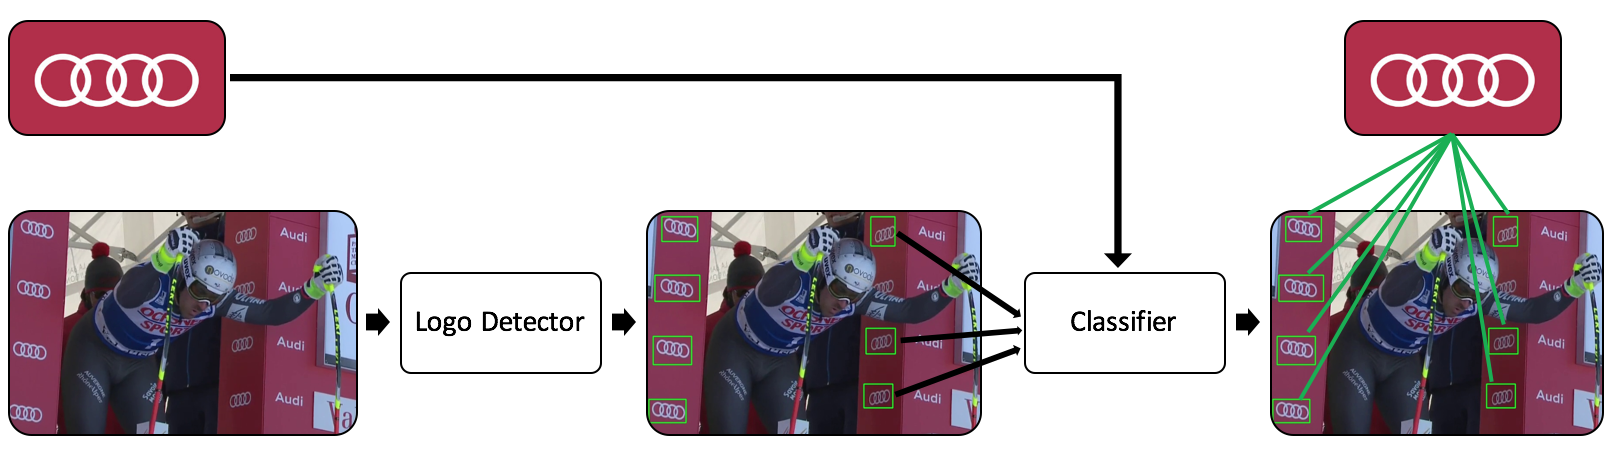
\includegraphics[width=12cm]{images/mt/outline.png}
	\caption{The outline of the proposed system}
	\label{f:outline}
\end{figure}
The challenge of this task is manifold. The first problem is that the logos in these videos are far from being perfectly clear. They can be partially occluded, blurred - if the camera moves fast, perspectively transformed, rotated and can have various coloring, suiting well to the design of the shirt or the arena. In addition, there is a problem with the ambient illumination variation just as for other computer vision tasks.
The second challenge is due to the legal prohibition of copying symbols. This already results in a huge appearance variety, which is further grown by the diversity of logos within a company. This makes the detection of logos very complex. In addition, a lot of companies use wordmarks i.e. a logo only with its name. For a system, not prepared for text recognition, it is a harder task to recognize complete words than only a letter or a simple graphic mark, symbol. These problems make the task of logo retrieval to an open-set recognition problem.
Furthermore, in classification tasks, the objects to be classified have usually a 3D shape in the reality, whereas logos have only a planar surface. It means, that it does not yield additional information, if a logo is photographed from multiple different angles, unlike in case of other objects.
Unfortunately, there are only a few publicly available small datasets with bounding box annotated logos. The majority of the images are adjusted to ensure a good visibility of the logos, unlike on the frames of the sport videos.
Figure \ref{f:challenges} introduces some examples of the challenges.
\begin{figure}
  \centering
  \begin{tabular}{ccccc}
  
\includegraphics[height=15mm]{images/mt/challenge_1_a.png} &   
\includegraphics[width=25mm]{images/mt/challenge_2_a.png}  & 
\includegraphics[width=25mm]{images/mt/challenge_3_a.png} &   
\includegraphics[width=25mm]{images/mt/challenge_4_a.png} & 
\includegraphics[width=25mm]{images/mt/challenge_5_a.png} \\
    
\includegraphics[width=25mm]{images/mt/challenge_1_b.png} &   
\includegraphics[width=25mm]{images/mt/challenge_2_b.png}  & 
\includegraphics[width=25mm]{images/mt/challenge_3_b.png} &   
\includegraphics[width=25mm]{images/mt/challenge_4_b.png}  & 
\includegraphics[width=25mm]{images/mt/challenge_5_b.png} 
    \end{tabular}
    \caption{Examples for challenging logos, where the instances of each column belong to the same class}
    \label{f:challenges}
\end{figure}
To master these challenges, the available solutions and methods improved a lot recently. In the decade before, hand-crafted feature extraction was prevalent in computer vision tasks. It needed an expert to create a system and it yielded often only mediocre results. Deep learning methods for computer vision problems have been dominant since the success of Convolutional Neural Networks in 2012 \cite{NIPS2012_4824}. Compared to earlier systems (e.g. Scale and Translation Invariant Features \cite{Lowe:2004:DIF:993451.996342}, Histogram of Oriented Gradients \cite{Dalal:2005:HOG:1068507.1069007} features), the great improvement of deep learning methods is the capability of learning how to extract features automatically. The enhancements are encouraged by continuous research. The development of deep nets is mainly powered by the annually organized ImageNet classification challenge \cite{ILSVRC15}. Since the aim of this contest is to classify an object, which fills out the majority of an image, the location of the particular object is irrelevant. To be able to classify and recognize objects, which have a much smaller size relative to the size of the whole image, region-based classification can be utilized.
\bigbreak
The rest of this thesis is organized as follows. Chapter \ref{c:relatedwork} reviews the related work of image retrieval, object detection and logo retrieval. In chapter \ref{c:theory} the proposal based object detection with Convolutional Neural Networks will be introduced. Chapter \ref{c:logoretrievalsystem} describes the logo retrieval system. Chapter \ref{c:experiments} presents some experiments to extend the size of the dataset, and evaluates different methods on a standard dataset. Afterwards, chapter \ref{c:evaluation} includes evaluation and comparison of the system with another logo retrieval methods. Finally, the last chapter concludes the work and gives prospects on future work.
\chapter{Related Work}\label{c:relatedwork}

This chapter gives an outline on the recent research related to this work. The included topics are deep learning, object detection, image retrieval, open-set classification and logo retrieval.
Deep neural networks are motivated by the memorization procedure of the human brain. Rosenblatt invented perceptrons \cite{Rosenblatt58theperceptron:}, which serve as the basis of today's Fully Connected layers (FC) in deep learning. LeCun applied \cite{LeCun:1989:BAH:1351079.1351090} Convolutional Neural Networks (CNN) for handwritten digits recognition in 1989, which are inspired by the visual cortex of the nervous system. Since then, a lot of research was made to improve and extend the application scope of deep learning in computer vision.
\section{Object Detection}
Earlier systems utilized hand-crafted features to detect objects on images and recognize them. Lowe et al., used Scale and Translation Invariant Features (SIFT) \cite{Lowe:2004:DIF:993451.996342} around keypoints, detected with e.g. Harris corner detector \cite{Harris}. Viola and Jones utilized \cite{Viola:2004:RRF:966432.966458} Haar-like features and a cascade of weak classifiers (Adaptive Boosting \cite{Schapire:1999:BIB:1624312.1624417}) to detect faces extremely fast. Nowadays, deep learning methods surpass the traditional methods by a wide margin. OverFeat framework \cite{journals/corr/SermanetEZMFL13} uses sliding windows on multiple scales of the image, and combines the features to detect objects and to classify them. You Only Look Once (YOLO) \cite{DBLP:journals/corr/RedmonDGF15} introduces an end-to-end network for detecting and classifying objects by using bounding box regressors at the first time for localization. It splits the input image into a square grid, where every cell predicts several bounding boxes with probability scores and classification labels. The Single Shot MultiBox Detector (SSD) \cite{journals/corr/LiuAESR15} utilizes convolutional features from multiple layers and concatenates them to detect objects in real time. Faster Region-Based Convolutional Neural Network (R-CNN) \cite{NIPS2015_5638} will be detailed in chapter \ref{c:theory}. Region-based Fully Convolutional Network (R-FCN) \cite{DBLP:journals/corr/DaiLHS16} is the improvement of Faster R-CNN in terms of inference time by having a network end-to-end fully convolutional. Mask R-CNN \cite{he2017maskrcnn} extends the functionality of Faster R-CNN by extending the network with a classification mask, which allows end-to-end object detection and semantic segmentation with a little overhead.
\section{Image Retrieval}
Many techniques exist outside the scope of deep learning for image retrieval from videos. SIFT features \cite{Lowe:2004:DIF:993451.996342} with bag-of-visual-words were used to get translation invariant descriptors around keypoints by Zisserman \cite{Sivic:2003:VGT:946247.946751}. The visual words were then used to retrieve objects in videos instantaneously like searching on Google. Histogram of Oriented Gradients (HOG) \cite{Dalal:2005:HOG:1068507.1069007} descriptors are gradient orientation histograms, extracted blockwise as features. Hu et al. \cite{Hu:2013:PEG:2479988.2480107} used an extended version of HOG descriptors to retrieve images based on sketches from a database. Nowadays, deep learning approaches are prevalent in the context of image retrieval. In \cite{Yan:2016:CVS:2964284.2967252}, CNN and SIFT features were compared and fused to retrieve images. Babenko et al. \cite{DBLP:journals/corr/BabenkoSCL14} utilized the output of the middle fully connected layer to retrieve images taken in same or similar scenes. This approach is used also in this work, however Babenko used the complete image as input, not low resolution Region of Interests (RoIs). Gordo et al. \cite{DBLP:journals/corr/GordoARL16} extracted local features from different regions of an image, which are selected by a region proposal system, and combined them to a global feature to retrieve images with similar scenes. In \cite{DBLP:journals/corr/RadenovicTC16} Maximum Activations of Convolutions (MAC) was computed from the output of a Fully Convolutional Network to represent images. MAC is a max pooling from the two dimensions of each channels, then the max value of every channel is used as a feature.
\section{Open Set Classification}
Bendale et al. argue \cite{DBLP:journals/corr/BendaleB15} with the fact that the majority of proposed neural networks utilize softmax layer to get classification probabilities. Thus, these networks are inherently trained for a closed-set classification world. These models can easily be fooled with abstract images, humans easily reject from any of the trained classes, but with the network predicting a class label with high probability. For this purpose, they propose OpenMax, which can be used to replace the softmax layer. OpenMax is able to classify such fooling and adversarial images as unknown.
\section{Logo Retrieval}
Romberg et at. \cite{Romberg:2011:SLR:1991996.1992021} published FlickrLogos-32 dataset, which became the standard evaluation dataset of logo retrieval systems. Furthermore, Romberg et al. \cite{conf/mir/RombergL13} generated synthetic data to increase the training dataset size, and combined local features from logo images into an aggregated feature. Pandey et al. \cite{DBLP:conf/icip/PandeyDJPB14} used SIFT features and bag-of visual words to retrieve logos from natural images, where the logo filled the complete image. In \cite{DBLP:journals/corr/HoiWLWWXW15} a large logo dataset of 100 brands with about 130,000 instances was introduced, which is unfortunately still not publicly available. In \cite{Eggert:2015:BSD:2733373.2806407}, synthetic logo dataset was utilized and a neural network was trained with unlabeled data by bootstrapping. Iandola et al. \cite{DBLP:journals/corr/IandolaSGK15} used Fast R-CNN for the first time to retrieve logos from images. Furthermore, R-CNN, Fast R-CNN and Faster R-CNN were used in \cite{Bao:2016:RCL:3007669.3007728}, \cite{DBLP:journals/corr/OliveiraFPR16}, \cite{DBLP:journals/spl/QiSWX17}. In \cite{DBLP:journals/corr/SuZG16} synthetic logo data was used to extend a train dataset with very scarce size. In 2017 Bianco et al. introduced Logos-32Plus \cite{bianco2017deep}, which is currently the largest publicly available dataset with 12,312 RoIs altogether.
\chapter{Proposal Based Object Detection and Classification}

In this section the theoretical overview of the logo retrieval system will be presented. First of all the fully convolutional networks will be introduced in section \ref{s:c-fullyconvnet}. Section \ref{s:c-rpn} explains region proposal systems for generating candidate object locations on an image. Afterwards, the section \ref{s:c-rcnn} describes region based convolutional neural networks for object detection and classification. The improvement of this method, the fast region based convolutional neural networks will be detailed in the section \ref{s:c-fastrcnn}. Folowing this, the further development, the faster region based convolutional neural networks will be reviewed in the section \ref{s:c-fasterrcnn}.

\section{Fully Convolutional Neural Networks}\label{s:c-fullyconvnet}
A neural network is fully convolutional, if it does not contain any fully connected layers. Firstly Matan et.al. used FCNs for recognizing strings of digits. Long et. al. proposed \cite{DBLP:journals/corr/LongSD14} how to transform a deep neural network with fully connected classifier layers at the end, to a fully convolutional network. For this purpose the fully connected layers at the end of the network are to be converted to convolutional layers.
\smallbreak
Since the number of weights of a neuron in a fully connected layer is defined by the shape of the data of the layer, the trained network can process only a fix-sized input. As a fully convolutional network does not have fully connected layer anymore, it has the advantage of being able to train and test with images of arbitrary sizes.
\smallbreak
The outputs of such a network are two dimensional feature maps, which can be used as heatmaps per class. These convolutional maps can also be used directly for semantic segmentation, where each pixel of an image should be classified.
Nowadays fully convolutional networks are essential part of state-of-the-art object detectors, yielding better performance, image size agnosticism, as well as shorter training and inference times.

\section{Region proposal systems}\label{s:c-rpn}
To recognize different objects on an image, like logos, small regions should be considered. The easiest way to search for these locations is the exhaustive sliding window search, applied on multiple scales. Although, as section \ref{s:c-objectdetection} presents, this induces a lot of computational costs. In order to reduce this computational burden, region proposal systems can be utilized. Region proposals are possible object locations on an image.
\smallbreak
Earlier computer vision solutions used external proposal systems. This means that the proposals of every image should be pre-calculated before training or inference. One of the most popular region proposal methods is selective search \cite{Uijlings13}. It merges neighbor regions according to a similarity score in a bottom-up fashion. It processes an image under 2s on the CPU, which precludes the possibility of real time applications. Edge Boxes \cite{edge-boxes-locating-object-proposals-from-edges} are efficiently calculating the number of contours in a box, and ranking them according to that almost real time. Today, as section \ref{s:c-fasterrcnn} introduces, the proposal system is already part of the neural network.

\section{Region Based Convolutional Neural Networks}\label{s:c-rcnn}

This section gives a brief overview about how faster region based convolutional neural networks evolved.

\subsection{Regions with Convolutional Neural Network Features}
Although this network is already historical, it is worth to mention it, because it helps to understand the improvements of the later systems. Region based convolutional neural networks \cite{DBLP:journals/corr/GirshickDDM13} consist of three separate systems. Firstly, region proposals are generated external with selective search. There will be altogether 2000 object positions considered. Secondly, each region of the possible object locations is warped to a size of 227x227, and then the feature vector of every single region is extracted with a CNN. The network is pretrained on the ImageNet dataset \cite{NIPS2012_4824}, and then fine-tuned on the final classes. The network is run on every region proposal bounding boxes, to extract vectors with a fixed-size. These vectors will to be written to the disk. Thirdly, a set of class-specific linear SVM is used to classify the specific region.

\subsection{Fast Region Based Convolutional Neural Network}\label{s:c-fastrcnn}
Fast Region based CNNs \cite{Girshick:2016:RCN:2881668.2882239} are aimed to improve the classification accuracy and feature vector extraction speed of the interesting regions, generated also with selective search. An intermediate convolutional feature map is extracted from the whole input image with a fully convolutional neural network, also called as base network in \citep{journals/corr/SermanetEZMFL13}. The output is a downscaled feature map, which is fed to the so called RoI (region of interest) pooling layer. This layer crops regions from the map according to the appropriate downscaled region proposals, and executes a modified version of max pooling on each regions, which results in a convolutional map with a fixed-shape, regardless the size of the region.

After the pooling, fully connected layers are used to calculate the final class probabilities and bounding box regressions for each region. The output of the bounding box regression are class specific small position and size adjustments, needed to refine the rough object locations.
\smallbreak
The improvements of this method compared to the previous region based CNN introduced in section \ref{s:c-rcnn} are as follows:
\begin{itemize}
	\item\textbf{Joint inference:} much shorter training and inference time is achieved by the lower computational redundancy of running convolutional layers on the whole image only once, rather then for every proposed regions.
	\item\textbf{One network:} the feature extraction and the classification happens in the same network. This has more advantages:
	\begin{itemize}
	        \item This results again in faster test and training times, due to the unnecessity of writing the extracted feature vectors to disk, which incidentally could require hundreds of gigabytes of storage \cite{Girshick:2016:RCN:2881668.2882239} for the VOC07 trainval set \cite{pascal-voc-2007}.
	        \item As the backpropagation is implemented through the RoI pooling layer, the whole network, together with the convolutional layers, can be trained jointly, against earlier implementations, like R-CNN \cite{DBLP:journals/corr/GirshickDDM13} or spatial pyramid pooling networks (SPPnet) \cite{DBLP:journals/corr/HeZR014}.
	\end{itemize}
	\item\textbf{Minibatch from a few images:} Faster training speed is achieved by collecting a minibatch only from two images, rather than every region from different images. This method is proved to converging within similar times, despite the high correlated regions.
\end{itemize}
The network is trained with a multi-task loss function for classification and bounding box regression, defined as:
\begin{equation}\label{eq:c-frcnn-loss}
	L(p, u, t^u, v) = L_{cls}(p, u) + \lambda [u \ge 1] L_{loc}(t^u, v)
\end{equation}
where $p$ is the computed class probabilities, $u$ is the groundtruth class, $t^u$ is the predicted bounding box offsets for every classes, and v is the groundtruth bounding box position and size.
Since the probabilities are calculated with softmax as usual, the log loss is used for the classification error: $L_{cls}(p,u) = -logp_u$. For bounding box regression loss, a smooth version of L1 loss is used, which is defined as follows:
\begin{align}\label{eq:c-smoothl1loss}
	L_{loc}(t^u, v) = \sum\limits_{i \in (x, y, w, h)} smooth_{L_{1}} (t_{i}^u, v_i)\\
	smooth_{L_{1}} (x) = \begin{cases}
               0.5 x^2 & \text{if } \abs{x} < 1\\
               \abs{x}-0.5 & \text{otherwise}
            \end{cases}
\end{align}
 is As the background class has the 

The network is trained for K+1 classes, where K is the number of object classes, and the background is also modelled as a separate class. During training, the positive examples are chosen, regarding the intersection over union (IoU) value to the groundtruth. This value is widely used for measuring the overlapping between regions, regardless the actual size of the regions. The calculation between two regions, $R_1$ and $R_2$ is as follows:
\begin{equation}\label{eq:c-iou}
        \frac{area ( R_1 \cap R_2 )}{area ( R_1 \cup R_2 )}
\end{equation}
For positive training examples there are thoose regions applied, which have an IoU with the groundtruth at least 0.5. For the background class are the examples with IoU [0.1,0.5) used.

\subsection{Faster Region Based Convolutional Neural Network}\label{s:c-fasterrcnn}

A great disadvantage of the Fast R-CNN method is, that the region proposals are generated externally. Girshick et.at. introduces Faster R-CNN \cite{NIPS2015_5638}, which generates the interesting regions within the neural network nearly cost-free (10ms pro image). This system consists of a region proposal system and a Fast R-CNN object detector.

\subsubsection{Region Proposal Network}

The convolutional feature map, extracted by the base network, is processed by the RoI pooling layer. Additionally a thin fully convolutional network, the region proposal network (RPN), is also utilized on the convolutional maps, to generate the proposals. Reference boxes, called "anchors" are generated at every position of the conv feature map, in different scales and different aspect ratios. This ensures the scale invariance of the objects. A convolutional layer with 3x3 kernel extracts a fixed-size vector from every window of the conv map, where in each window 9 anchors are considered. As the fully convolutional network iterates through the conv map in a sliding window fashion, translation invariance is granted. An objectness score and bounding box offset is then calculated for every anchor, by different classifiers and regressors, specialized in a specific scale and aspect ratio.

\subsubsection{Training}

As the RPN is a class agnostic object detector, it should detect all the types of objects, which the network is trained on. For this purpose, the class informations, during training of RPN, can be discarded. Positive examples are collected from the proposals with an IoU higher than 0.7 with any groundtruth. Negative label is assigned for regions, which have an IoU, lower than 0.3.

Since the objective of the RPN is the same as for Fast R-CNN, namely to classify regions and regress bounding box coordinates, the loss functions for training the RPN can the same multi-task loss, which are used for training a Fast R-CNN, detailed in section \ref{s:c-fastrcnn}.
\chapter{Logo Retrieval System}

\section{Logo Datasets}
The hunger of deep learning method for training data is well-known. As the publicly available logo datasets are quite small, a better training result can be achieved if the datasets are merged. The different datasets with the number of brands, images and bounding box rois can be seen in table \ref{table:logodatasets}. The total number of brands means the number of different brands altogether.

There are also trademark datasets available having a much greater cardinality \cite{DBLP:journals/corr/TursunAK17}. The images of this dataset contain however only the logo of a company, without any context of the logo. This dataset turned out to have no use for region based deep learning methods, since this approach needs to learn to distinguish between objects to be learned and the background. The network was trained with the fusion of FlickrLogos-32 and the trademark dataset, and tested with the evaluation method of FlickrLogos-32.
\begin{table}[ht!]
\centering
\caption{Publicly available logo datasets with with bounding box annotations}
\label{table:logodatasets}
\begin{tabular}{|l|l|l|l|}
\hline & \textbf{Number of brands} & \textbf{Number of logo images} & \textbf{Number of ROIs} \\
\hline
\textbf{BelgaLogos} & 37 & 1321 & 2697 \\
\hline
\textbf{Flickr Logos 27} & 27 & 810 & 1261 \\
\hline
\textbf{FlickrLogos-32} & 32 & $70 \cdot 32 = 2240$ & 3404 \\
\hline
\textbf{Logos-32plus} & 32 & 7830 & 12300 \\
\hline
\textbf{TopLogo10} & 10 & $10 \cdot 70 = 700$ & 863 \\
\hline\hline
\textbf{Total (union)} & \textbf{80} & 12 901 & 20 525 \\ \hline
\end{tabular}
\end{table}

\section{Logo Detection}

supervised pre-training on a large auxiliary dataset (ILSVRC), followed by domain- specific fine-tuning on a small dataset (PASCAL), is an effective paradigm for learning high-capacity CNNs when data is scarce. RCNN paper \cite{DBLP:journals/corr/GirshickDDM13}

\section{Logo Comparison}

Krizhevsky?s CNN can be used (without fine- tuning) as a blackbox feature extractor, yielding excellent performance on several recognition tasks work by Donahue et al. \cite{DBLP:journals/corr/DonahueJVHZTD13}

\chapter{Experiments}

Precision and recall are favoured values in image retrieval. Precision is the fraction of relevant retrieved objects and all the retrieved objects. Recall is the ratio of relevant retrieved objects to all the relevant objects. Although, many retrieval system is capable to return a ranked list of the retrieved objects, precision and recall ignore this information. Thus, the trained models are evaluated with the nowadays very popular mean average precision (mAP) metric. In particular, a descending sorted list will be created for every company, based on the probabilities of being logos from the specific brand on given positions of the images. Firstly the precision curve as a function of recall is acquired for every list. The average precision is then calculated as the area under the precison-recall curve. The average of these values gives the mean average precision.
All the mentioned results will be calculated with the evaluation implementation of py-faster-rcnn \cite{Girshick2017} \cite{NIPS2015_5638}.

\section{Training with Synthetic Data}

\subsection{FlickrBelgaLogos dataset}

A dataset, which is annotated manually, may contain logos, which stay unannotated. If a system is evaluated on such a dataset, and finds the unannotated logo, it counts as false positive detection. Thus, a synthetic dataset, called FlickrBelgalogos \cite{letessier2012scalable} is created for evaluation purpose, by pasting the logo annotations of the dataset BelgaLogos \cite{belgalogos09} on images from Flickr to random positions. One could argue with the correctness of evaluating a detector with this dataset, because alone the contrast difference may make the logos easier to detect on these images.

This dataset was evaluated for training purposes. Therefore a small subset of BelgaLogos was chosen as test set

\subsection{METU Trademark dataset}

To try to increase the size of training dataset, a synthetic dataset was generated, where one logo from the METU Trademark dataset \cite{DBLP:journals/corr/TursunAK17} was placed on an image. As basis, images from Tripadvisor were used. There are some transformations, which were applied on the logo images before. The majority of the logo's background has a white color. Thus one third of the dataset is left original. The brightness of the rest of them was adjusted to the brightness of the image on which the logo is placed, and for one third of the logos the mean hsv value of the logo is calculated and rotated with 90 degree chosen randomly. The table \ref{table:logotransformations} summarizes the applied transformations.

\begin{figure}
  \centering
\begin{tabular}{cccc}
  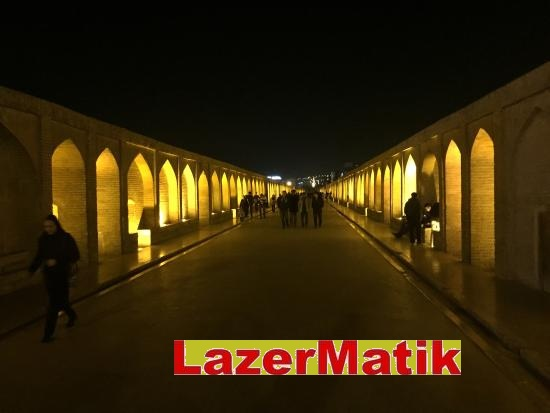
\includegraphics[width=25mm]{images/mt/synmetu1.jpg} &   
\includegraphics[width=25mm]{images/mt/synmetu2.jpg}  & 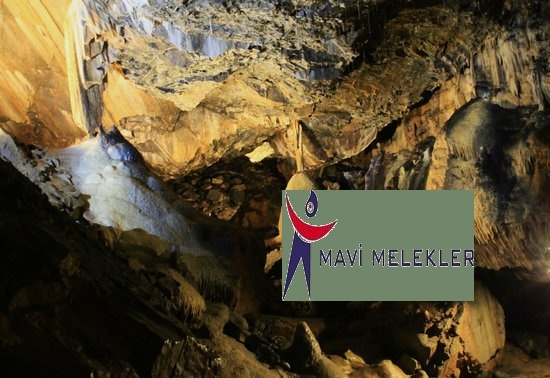
\includegraphics[width=25mm]{images/mt/synmetu3.jpg} &   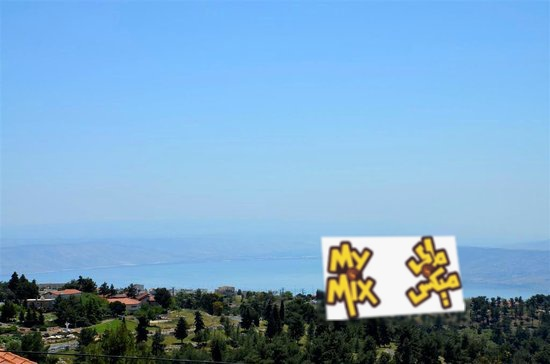
\includegraphics[width=25mm]{images/mt/synmetu4.jpg} \\
    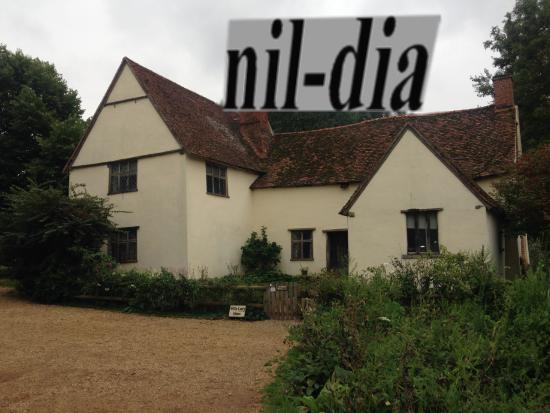
\includegraphics[width=25mm]{images/mt/synmetu5.jpg} &   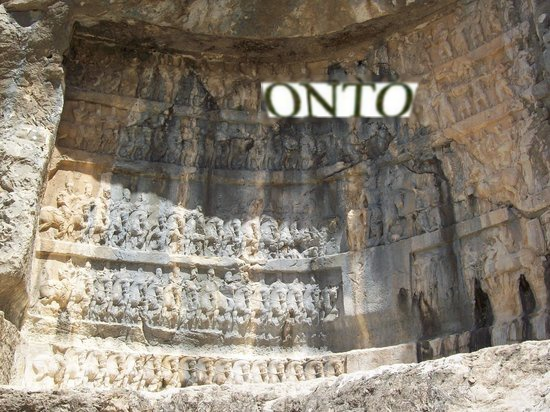
\includegraphics[width=25mm]{images/mt/synmetu6.jpg}  & 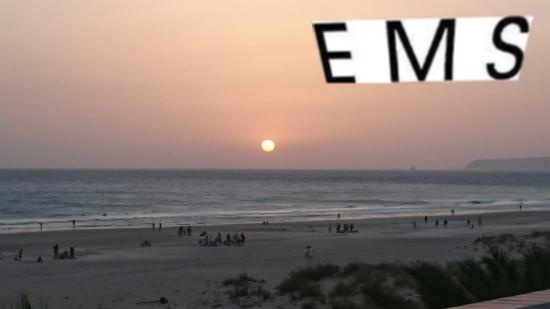
\includegraphics[width=25mm]{images/mt/synmetu7.jpg} &   
\includegraphics[width=25mm]{images/mt/synmetu8.jpg} 
\end{tabular}
\caption{Generated synthetic logo images}
\end{figure}

\iffalse

\begin{table}[ht!]
\centering
\caption{Applied transformations}
\label{table:logotransformations}
\begin{tabular}{|c|c|c|}
\hline & \textbf{Brightness adjustment} & \textbf{Hue rotation} \\
\hline
\textbf{33\%} & - & - \\
\hline
\textbf{33\%} & yes & yes \\
\hline
\textbf{33\%} & yes & yes \\ \hline
\end{tabular}
\end{table}

\fi






\section{Logo Detection}



\section{Logo Retrieval}

\chapter{Conclusion}

\section{Summary}

\section{Future Work}


%% F?r die Verwendung mit includeonly s?he es so aus. Und falls man chapterbib verwenden will
%%\chapter{Anleitung zur \LaTeX-Vorlage}

\lettrine[nindent=0.2em]{H}{erzlich Willkommen} zur \LaTeX-Vorlage des IES. Wir freuen uns, dass Sie sich f�r diese Vorlage entschieden haben, denn damit bringen Sie zum Ausdruck, dass hochwertige Druckerzeugnisse f�r Sie von Belang sind.

Diese Vorlage basiert in ihren Grundz�gen auf der exzellenten \enquote{allgemeinen sehr umfassenden} Vorlage von Matthias Pospiech (\url{http://www.matthiaspospiech.de/latex/vorlagen/}). Ohne diese Basis w�re die Vorlage niemals das geworden, was sie ist. Vielen~Dank!

\section{Voraussetzungen}

Zun�chst eine Liste der technischen Voraussetzungen um diese Vorlage nutzen zu k�nnen.

\begin{itemize}
	\item Windows-PC mit \LaTeX-Distribution (Getestet ist Win XP SP3 und Win 7 64-bit jeweils mit MikTeX\footnote{\url{http://www.miktex.org/}} 2.9)
	\item Internetanschluss zum dynamischen Nachladen der Pakete
	\item \LaTeX-Entwicklungsumgebung wie \zb TeXnicCenter\footnote{\url{http://www.texniccenter.org/resources/downloads/29}} (TXC), Winshell\footnote{\url{http://www.winshell.org/modules/ws_download/}}, WinEdt\footnote{\url{http://www.winedt.com/}} (Shareware)
	\item Sync\TeX-f�higen PDF-Viewer wie \zb SumatraPDF\footnote{\url{http://blog.kowalczyk.info/software/sumatrapdf/download.html}}
	\item Ghostscript (bei MikTeX schon dabei)
	\item Optional: Perl-Installation
\end{itemize}

Die Vorlage ist speziell f�r Windows angepasst und auch nur dort getestet, sollte aber auch au�erhalb von Windows funktionieren.

\subsection{Mik\TeX-Einstellungen}
Bitte stellen Sie bei Mik\TeX ein, dass Pakete ohne Nachfrage vom Internet nachgeladen werden. Dies geschieht entweder bei der Installation oder ist zu finden im Startmen� unter MikTeX, Maintenance (Admin), Settings (Admin), General, Package installation, Install missing packages on the fly: Yes. Wird dies vers�umt kann das zu Fehlermeldungen im TXC f�hren (\enquote{GUI framework cannot be initialized}, v.a. bei �lteren MikTeX-Installationen). Bekommt man trotzdem noch diese Fehlermeldung kann man in der pdf\LaTeX-Befehlszeile noch \texttt{--enable-installer} hinzuf�gen, was Vorrang vor der Mik\TeX-Option hat. Hilft das auch nicht, kann man noch die aktuelle Alphaversion vom TeXnicCenter probieren oder Mik\TeX mal neu installieren.

Am IOSB muss man f�rs Mik\TeX-Update auch einen Proxyserver einstellen:\\
 \texttt{mca-01.iosb.fraunhofer.de} mit Port \texttt{3128}\\
Wird das nicht gemacht, k�nnen ben�tigte Pakete nicht nachgeladen werden.

Nach der Mik\TeX-Installation sollte man im Startmen� gleich \texttt{Update (Admin)} aufrufen, den Proxy eintragen und das Update machen lassen.

\subsubsection{Schriftart Libertine}

Inzwischen wurde bei Mik\TeX einiges umgestellt, was zur Folge hat, dass es Probleme mit der Schrift Libertine geben kann, die in der Vorlage f�r die �berschriften verwendet wird.

Hintergrund ist der, dass das Libertine-Paket inzwischen nur noch Schriften im OTF-Format enth�lt und daher wird in der Fehlermeldung auch empfohlen, das (neue) Paket
\texttt{libertineotf} zu verwenden.

Dieser Hinweis hilft aber nur dann, wenn man mit XeTeX oder LuaTeX arbeitet, was von uns aber glaube ich niemand tut. F�r die normalen pdfTeX-Anwender gibt es inzwischen Abhilfe durch das Paket \texttt{libertine-legacy}. Zumindest unter MikTeX gibt es da aber Schwierigkeiten bei der Umstellung, weil MikTeX automatisch das (inzwischen) nicht mehr geeignete \texttt{libertine} Paket auf der Suche nach der Schrift nachl�dt (wenn die Auto-Updates an sind) aber in dem Paket nicht das Richtige findet.

LaTeX-Guru Ulrike Fischer hat aber eine L�sung f�r uns parat:

\begin{quotation}
Wenn du pdflatex benutzt, solltest du im tex/latex/libertine-Ordner die Datei libertine.sty umbenennen oder l�schen, danach installiere das Paket libertine-legacy. Eventuell musst du danach noch die FNDB als User+Admin aktualisieren. Achte bei ersten Tests darauf, dass on-the-fly-Installation abgeschaltet ist, damit miktex nicht wieder die libertine.sty im libertine-Ordner neu installiert, sondern die in libertine-legacy n�tzt.
\end{quotation}

Erg�nzungen dazu von meiner Seite:

\begin{enumerate}
	\item Der genannte tex/latex/libertine-Ordner muss nicht der Order in \enquote{Program Files} sein, es wird oft der Ordner in den Benutzerdaten sein (manchmal gibt es das \texttt{libertine}-Paket vielleicht auch in beiden Ordnern):\\
	Unter XP sowas wie:\\
	{\tiny \verb+C:\Dokumente und Einstellungen\[username]\Anwendungsdaten\MiKTeX\2.9\tex\latex\+ }\\
	Unter Win7 ist es dann glaub so:\\
	{\scriptsize \verb+C:\user\[username]\Roaming\AppData\MiKTeX\2.9\tex\latex\+} \\
	(Ich bin mir nicht sicher, ob nur das Roaming-Profil betroffen ist oder auch das Local-Profil. Im Zweifel nach den libertine-Dateien suchen)\\
	
	\item Ulrike Fischer sagt \enquote{eventuell die FNDB updaten}. Nicht eventuell, sondern macht das! Startmen�, Maintenance, Settings, einmal als Admin und einmal nicht.
	\item Den Ordner \enquote{libertine} (in dem die \texttt{libertine.sty} enthalten ist) \emph{umzubenennen} hilft nichts, das FNDB-Update findet die \texttt{libertine.sty} trotzdem.
	\item In der Vorlage hei�t es nach wie vor \verb+\usepackage{libertine}+, NICHT \verb+\usepackage{libertine-legacy}+! Mit dem legacy-Paket wird die Schrift installiert und dann wird sie auch gefunden.
	\item Wenn die Kompilation dann geklappt hat, kann man die Auto-Updates in MikTeX wieder an machen.
\end{enumerate}



\subsection{SumatraPDF}
In SumatraPDF selbst muss nichts eingestellt werden. SumatraPDF ist von Haus aus Sync\TeX-f�hig. Das bedeutet, dass man (im Zusammenspiel mit den von pdf\LaTeX\ erzeugten Sync\TeX-Informationen) durch Doppelklick an einer beliebigen Stelle im PDF-Dokument zum zugeh�rigen \LaTeX-Codeblock im TXC springen kann. Umgekehrt springt SumatraPDF durch Dr�cken von F5 im TXC an die n�chstgelegene Stelle im PDF. Besonders im Zwei-Monitor-Betrieb kann man so bequem Korrekturlesen und gleich die entsprechenden Teile im Code korrigieren.

\subsection{TeXnicCenter-Einstellungen}
Vorab: Die hier genannten Aussagen gelten gleichsam f�r TXC 1{.}0RC1, die derzeit (August 2012) als stabil deklarierte Version von TXC. In der aktuellen Alpha4-Version von TXC 2{.}0 sehen viele Einstellungsdialoge aber identisch oder zumindest sehr �hnlich aus, so dass das Vorgehen ganz �hnlich mit nur kleinen Transferleistungen zu bewerkstelligen ist.

\subsubsection{TXC Alphaversion und Windows 7}
Unter Windows 7 (insbesondere den 64-bit-Versionen) scheint TXC 1{.}0RC1 nicht zuverl�ssig zu funktionieren, was das automatische Nachladen der Pakete betrifft. Auch die Inverssuche mit SumatraPDF scheint nicht reibungslos zu klappen. Daher der Hinweis, speziell unter Windows 7 die Alphaversion von TXC zu verwenden, die in meinen pers�nlichen Tests genauso stabil ist wie die Version 1{.}0RC1. Auch unter Windows XP l�uft die Alphaversion sehr gut und ich ziehe sie der 1{.}0RC1 vor.

\subsubsection{Ausgabeprofile}
TeXnicCenter verwaltet den \LaTeX-Kompiliervorgang �ber sogenannte Ausgabeprofile. Dort wird festgelegt, mit welchen Parametern der pdf\LaTeX/pdf\TeX-Lauf, der Bib\TeX-Aufruf und der Aufruf des PDF-Viewers gestartet wird. Die folgenden Einstellungen gelten f�r SumatraPDF als Viewer.

Zuerst erstellt man sich zwei neue Ausgabeprofile: Eines f�r Einzeldokumente (eine \texttt{*.tex}-Datei f�r alles) und eines f�r TXC-Projekte (eine Hauptdatei, die andere \texttt{*.tex}-Dateien aufruft). Braucht man unterteilte Literaturverzeichnisse wird am besten noch ein drittes Profil angelegt, dazu sp�ter mehr.
Zu finden ist die Option im Men�: Ausgabe, Ausgabeprofile definieren (Alt+F7), Hinzuf�gen. Diesen Profilen gibt man beliebige aber sinnvolle Namen wie \zb \enquote{Sumatra EinzelTeX} oder \enquote{Sumatra Projekt} (oder \enquote{Sumatra Multi Literatur}). Die beiden Profile werden sich sp�ter nur um wenige Details unterscheiden, aber das reicht ja schon.

\paragraph{pdf\LaTeX} Pfad zu pdf\LaTeX: An die jeweilige Installation anpassen. Die Argumente f�r den Compiler sind:\\ {\tiny \verb+-synctex=-1 -interaction=nonstopmode -max-print-line=120 "%pm" --enable-write18+}\\
Die Optionen bedeuten, dass Sync\TeX-Informationen erzeugt werden sollen, dass der pdf\LaTeX-Lauf nicht mit Nachfragen an den Nutzer stoppt, erlaubt Compileausgaben bis 120 Zeichen pro Zeile und erlaubt \emph{Shell-Escape} (write18). Das ist eine besonders wichtige Option, denn ohne ihn k�nnen weder EPS-Grafiken oder psfrag verwendet werden noch k�nnen PDF-Grafiken automatisch zugeschnitten (gecroppt) werden.

\paragraph{Bib\TeX}
Verwendet man nur ein Literaturverzeichnis, muss man bei den Einstellungen zum Bib\TeX-Compiler nichts besonderes beachten: Den Pfad ggf. anpassen und als Argument nur \verb+"%bm"+.

Bei Problemen mit Bib\TeX\ was das Encoding angeht (Umlaute, Sonderzeichen), kann es helfen, die \texttt{bibtex8.exe} zu verwenden. Hintergrund: Bib\TeX\ stammt aus einer Zeit als 7-bit-Zeichens�tze (ASCII) g�ngig waren. BibTeX8 erweitert das auf 8-bit-Zeichens�tze. Evtl.\ �ndert sich die Sortierreihenfolge der Eintr�ge dadurch. Das Argument im TeXnicCenter lautet dann aber nicht mehr \verb+"%bm"+ sondern \verb+"%tm"+.

\paragraph{Bib\TeX mit mehreren Literaturverzeichnissen}
Verwendet man mehrere Literaturverzeichnisse (\zb getrennt nach Journals, Konferenzen und sonstigen Ver�ffentlichungen), wird der normale BibTeX-Lauf mit dem Haken bei \enquote{BibTeX in diesem Profil nicht verwenden} ausgeschaltet und es m�ssen gem�� der Anzahl der Literaturverzeichnisse einmalig im TeXnicCenter unter dem Reiter \enquote{Nachbearbeitung} zus�tzliche Bib\TeX-Postprozessoren mit dem Argument \verb+"%bm1"+ f�r das erste Verzeichnis und \verb+"%bm2"+ f�r das zweite \usw eingerichtet werden. F�r die Postprozessoren kann ebenfalls bibtex8 eingesetzt werden (entsprechend mit \verb+"%tm"+).

\paragraph{Makeindex}
Die Einstellungen f�r MakeIndex sind zu �ndern. Und zwar wird MakeIndex zweimal aufgerufen: Einmal, um das Symbolverzeichnis (die Nomenklatur) zu erstellen (was wir an dieser Stelle eintragen) und einmal, wenn ein Inhaltsverzeichnis (der klassische Index) gew�nscht ist. Diesen zweiten Aufruf werden wir sp�ter unter \enquote{Nachbearbeitung} eintragen.

\paragraph{Makeindex - Symbolverzeichnis}
Wir passen wieder den Pfad an, wo die \texttt{makeindex.exe} tats�chlich liegt und schreiben bei den Argumenten folgendes rein:\\
\verb+"%tm.nlo" -s nomencl.ist -t  "%tm.nlg" -o "%tm.nls"+

Das sollte dann so �hnlich aussehen wie in \ref{fig:TXCprofile}.

\paragraph{Makeindex - Index}
Wer beabsichtigt auch einen Index erzeugen zu lassen, sollte unter \enquote{Nachbearbeitung} noch einen Eintrag erstellen, der wiederum \texttt{makeindex.exe} aufruft, diesmal aber nur mit dem Argument \verb+"%bm.idx"+.
Man kann die \texttt{nomencl.ist} auch f�r deutsche Sortierung anpassen, indem man in der Datei zwei Prozentzeichen entfernt. Das ist in der Datei markiert und hei�t \enquote{Germans might want to change this and delete the two \%\%}

\paragraph{PDF Viewer}
Auf dem Reiter \enquote{Viewer} wird nun eingestellt, wie TXC mit SumatraPDF kommuniziert. Hier liegt auch die eigentliche Sync\TeX-Funktionalit�t begraben.

Als Befehlszeile wird folgendes eingetragen:\\
{\tiny \verb+c:\Programme\SumatraPDF\SumatraPDF.exe -reuse-instance -inverse-search "\"c:\Programme\TeXnicCenter\TEXCNTR.EXE\" /ddecmd \"[goto('%f','%l')]'\""+\\}
wobei der Pfad zum SumatraPDF wie auch der Pfad zur TeXnicCenter \texttt{*.exe}-Datei angepasst werden muss.
Unter Windows 7 64bit sieht das dann \zb so aus (nat�rlich ohne die Zeilenumbr�che):\\
{\scriptsize \begin{verbatim}
C:\Program Files (x86)\SumatraPDF\SumatraPDF.exe
-inverse-search "\"C:\Program Files (x86)\TeXnicCenter2\TeXnicCenter.exe\"
/ddecmd \"[goto('%f','%l')]'\""+\\
\end{verbatim}
}

Bei \enquote{Projektausgabe betrachten} steht als Kommandozeile nur \verb+"%bm.pdf"+ drin.

\enquote{Suche in Ausgabe} wird durch DDE-Befehle gel�st, hier steht\\
\verb+[ForwardSearch("%bm.pdf","%Wc",%l,0,0,1)]+ drin.

\emph{Server} ist \texttt{SUMATRA} mit \emph{Thema} \texttt{control}. Jetzt sind wir auch an dem Punkt, an dem sich die zwei Profile unterscheiden: Beim Projekt-Profil steht im DDE-Befehl \verb+%Wc+
 w�hrend beim Einzeldatei-Profil \verb+%nc+ steht.

Bei \enquote{Vor Compilierung schlie�en} stellen wir auf \enquote{Nicht schlie�en}. Im Gegensatz zum Adobe Reader (der auch gar kein Sync\TeX\ kann), kann das PDF im Sumatra einfach die ganze Zeit ge�ffnet bleiben!

Wer unbedingt den Adobe (Acrobat) Reader benutzen will, sollte beachten, dass sich in Version 10 die DDE-Server ge�ndert haben und inwischen acroviewR10 (f�r den Reader) bzw.\ acroviewA10 (f�r den vollen Acrobat) lauten.

Geschafft -- das war der schwierigste Teil der Einrichtung.

\subsubsection{Die erste Kompilierung}

Wird das Dokument nun zum ersten Mal kompiliert, dauert das eine Weile, da die ganzen noch fehlenden LaTeX-Pakete w�hrend der Kompilierung aus dem Netz geladen und installiert werden. Der erste Kompiliervorgang f�hrt wohl auch noch zu einer Fehlermeldung. Nach dem zweiten Durchlauf (es werden noch die Pakete \texttt{pdfcrop} und \texttt{preview} nachinstalliert) sollte es 0 Fehler geben. Viele Warnungen sind noch kein Grund zur Sorge.

Verwendet man mehrere Literaturverzeichnisse kann es bis zum f�nften Durchlauf brauchen, bis alle Literaturreferenzen korrekt aufgel�st sind.

Auch am Ende bleiben bei A5-Kompilierung noch \ca 23 Warnungen �brig. Dagegen kann man im Moment nichts tun, sollte aber auch kein Grund zur Beunruhigung sein.

\subsubsection{Textbausteine}

Es ist recht hilfreich sich bei einem l�ngeren Dokument im TXC eigene Textbausteine zu erschaffen, die man dann einfach einf�gen kann. Kandidaten daf�r sind \zb \verb+\begin{hidecomment} \end{hidecomment}+ oder \verb+\footnote{\url{ }}+, je nachdem was man eben oft braucht.

\subsubsection{Rechtschreibpr�fung in TXC}

TeXnicCenter verwendet die OpenOffice-W�rterb�cher. Diese kann man frei herunterladen und nachinstallieren.

{\small
\url{http://wiki.services.openoffice.org/wiki/Dictionaries}}

Wer will, kann auch \texttt{aspell} verwenden, was sich anscheinend bequem aus TXC heraus aufrufen l�sst. Hab ich aber noch nicht getestet.

{\tiny
\url{http://raschka.supersized.org/archives/8-Aspell-Rechtschreibkorrektur-mit-der-Latex-IDE-TeXnicCenter-unter-Windows-DE.html}
}

{\small
\url{http://csenk.de/2010/05/14/aspell-und-texniccenter/}
}

\begin{figure}[htb]
\Centering
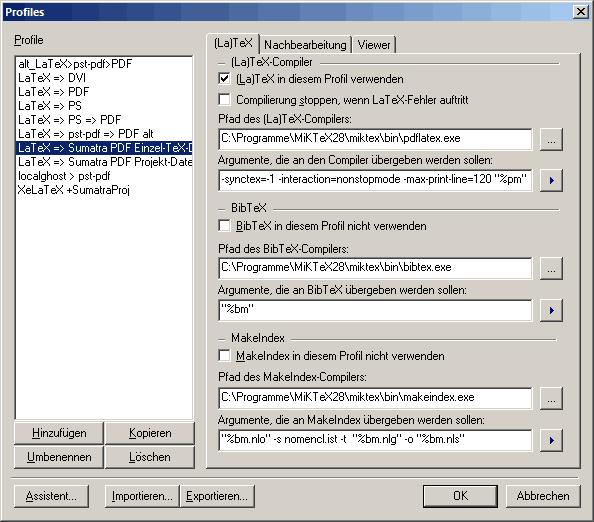
\includegraphics[width=0.6\textwidth]{images/anleit/sumaeinzel.png}
\caption{TXC-Screenshot der Ausgabeprofile}
\label{fig:TXCprofile}
\end{figure}


\begin{figure}[htb]
\Centering
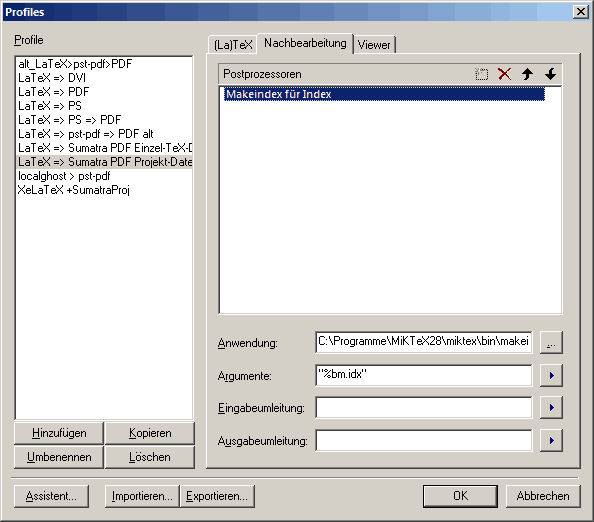
\includegraphics[width=0.6\textwidth]{images/anleit/txcmakeidx.png}
\caption{TXC-Screenshot der Nachbearbeitungsschritte}
\label{fig:TXCpostproc}
\end{figure}

\begin{figure}[htb]
\Centering
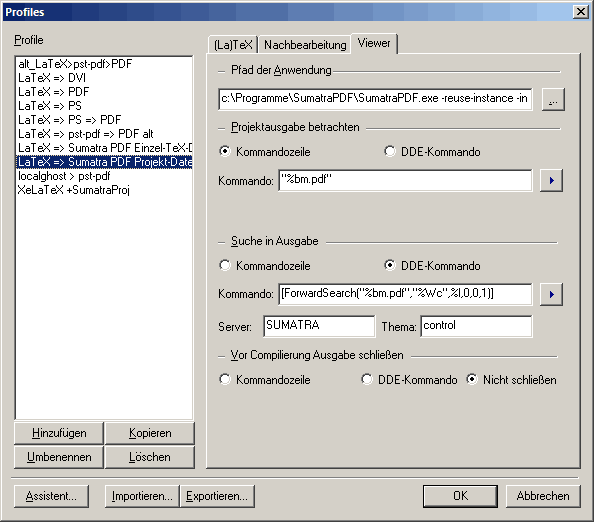
\includegraphics[width=0.6\textwidth]{images/anleit/txcviewer.png}
\caption{TXC-Screenshot der Viewer-Einstellungen}
\label{fig:TXCviewer}
\end{figure}

\subsection{Perl}

Es kann bei der Verwendung von \texttt{pstool} passieren, dass das erzeugte PDF falsch beschnitten wird. Das liegt daran, dass der ersetzte Text in der Regel mehr Platz beansprucht, als die gesetzten Platzhalter. Abhilfe schafft eine \texttt{pstool}-Option, die \texttt{pdfcrop} aufruft. Damit man beim pstool-Paket die Option \texttt{crop=pdfcrop} verwenden kann, muss im System Perl installiert sein, weil das externe Perl-Skript \texttt{pdfcrop} aufgerufen wird (bei Mik\TeX mit dabei). Das sorgt daf�r, dass die BoundingBox auch dann korrekt bestimmt wird, wenn durch psfrag-Ersetzungen die Grafik gr��er wird als sie vorher war.

Es funktioniert nach meinen Tests sowohl das Open-Source StrawberryPerl\footnote{\url{http://strawberryperl.com/}} als auch das f�r private Nutzung kostenlose aber kommerzielle ActivePerl\footnote{\url{http://www.activestate.com/activeperl}}. Strawberry Perl installiert sich standardm��ig direkt unter dem Wurzelverzeichnis, was meist unerw�nscht ist. Gegebenenfalls den Pfad �ndern.

Wer kein pstool verwendet (weil er kein psfrag und auch kein matlabfrag verwendet), braucht auch kein Perl zu installieren.

\subsection{Ghostscript}

Bei MikTeX wird eine Sonderversion von Ghostscript mitgeliefert. Ich finde, dass es f�r jeden, der mit \LaTeX\ arbeitet generell ratsam ist ein aktuelles Ghostscript\footnote{\url{http://www.ghostscript.com/}} mitsamt GSview\footnote{\url{http://pages.cs.wisc.edu/~ghost/}} installiert zu haben, sei es um PDFs mit einem anderen Viewer zu betrachten oder um irgendwelche Konvertierungen von Grafiken per Hand durchzuf�hren.

\section{Aufbau der Vorlage}

Die Vorlage basiert auf der �beraus gelungenen Vorlage von Matthias Pospiech, die schon sehr vieles vorbereitet hat. Auf seiner Homepage\footnote{\url{http://www.matthiaspospiech.de/latex/vorlagen/}} wird sie zum Download angeboten.

Die Vorlage besteht aus mehreren Dateien, die \textbf{Hauptdatei} ist die Datei \datei{LaTeX-Vorlage-IES.tex}. Diese kann umbennant werden, wobei ich sicherheitshalber keine Leerzeichen und keine Umlaute verwenden w�rde. Unter Windows ist es vermutlich auch ratsam, wenn der Dateiname zusammen mit dem Dateipfad 254 Zeichen nicht �berschreitet. Das entstehende PDF hei�t genauso wie die Hauptdatei. Die zugeh�rige TXC-Projektdatei (\texttt{*.tcp}) verweist unter Men�: Projekt, Projekteigenschaften auf die Hauptdatei.

Im Idealfall muss der Benutzer eigentlich nur in der Hauptdatei �nderungen machen. Die Hauptdatei ist kommentiert und unterst�tzt damit den Benutzer bei der korrekten Handhabung.

Schaut man sich die Hauptdatei an, f�llt auf, dass sie vergleichsweise kurz ist. Sie beinhaltet letztlich nur Verweise auf die verwendete Dokumentklasse (inklusive Papierformat und Schriftgr��e) und definiert Dokumentstruktur. Alle sonstigen Einstellungen und Inhalte sind in Extradateien ausgelagert. Zu Beginn wird die sehr umfangreiche Pr�ambel eingebunden. Dort werden die ganzen ben�tigten \LaTeX-Pakete geladen. Bei den Makros werden neue Befehle definiert oder vorhandene umdefiniert. Dann wird die Silbentrennungsdatei eingebunden (dazu sp�ter mehr).

Hinweis, wenn man selbst Dateien einbinden will: Benutze \verb+\include+ nur dann, wenn du \emph{wei�t}, dass \verb+\input+ nicht reicht.

Dann kommen Titel, Inhaltsverzeichnis, Symbolverzeichnis. Als n�chstes werden die eigentlichen Inhaltsdateien eingebunden. F�r jedes Kapitel eine. Das muss man nicht tun, aber es verk�rzt bei einem langen Dokument den Erstellungsvorgang stark, wenn man \zb nur das aktuelle Kapitel durchnudeln l�sst.

Am Ende kommen noch das Literaturverzeichnis sowie Abbildungs- und Tabellenverzeichnis gefolgt von einem Theoremverzeichnis und einem Verzeichnis der Codelistings. Nicht jeder ben�tigt alles davon. Was man nicht braucht, kann man hier (und nur hier) auskommentieren. Auskommentiert wird mit einem \%-Zeichen.

Die Pr�ambel bindet auch die Schriftartendefinitionen in einer Extradatei ein. Warnung: Schriftauswahl unter \LaTeX und insbesondere der Mathematiksatz ist ein bi�chen wie die H�lle auf Erden. Da gibt es zig Codierungen und virtuelle Fonts, die sich die ben�tigten Zeichen zusammensuchen. Au�erdem handhabt jedes Schriftpaket anders, welche Befehle und Zeichen umdefiniert werden. Das Schriftengebilde ist eine relativ fragile Konstruktion. Wer �nderungen vornimmt, sollte wissen was er tut.


\section{Hinweise zum Literaturverzeichnis}

Es gibt ein nicht einfach zu l�sendes Dilemma mit LaTeX und BibTeX:

M�glichkeit 1:\\Man macht die LaTeX-Dateien in UTF8, setzt die Option \texttt{utf8} beim \texttt{inputenc}-Paket und kann dann alle Zeichen als Eingabezeichen in den tex-Dateien verwenden. Dann muss man allerdings die bib-Dateien in ANSI lassen und Umlaute wie ein � so schreiben: \verb+{\"u}+.
Das ist bei der Vorlage Version 1.1 gerade der Fall.

M�glichkeit 2:\\Man beschr�nkt die LaTeX-Dateien auf beispielsweise \texttt{latin1} oder \texttt{latin9}, setzt die entsprechende \texttt{inputenc}-Option (kann dann nur die darin vorkommenden Zeichen verwenden) und hat dann die M�glichkeit, diese mit BibTeX bzw. BibTeX8 auch zu verwenden. Allerdings ist das wohl auch nur halboffiziell m�glich und es gibt keine Garantie, dass es l�uft.
So war es bei der Vorlage in Version 1.0.

Beide L�sungen sind nicht das Gelbe vom Ei, aber je nachdem wie es einem lieber ist, kann man sich auch Vorlage 1.1 wieder auf \texttt{latin9} zur�ckstellen.

Eine L�sung w�re der komplette Verzicht auf BibTeX und Umstieg auf biblatex, aber das ist eher f�r Version 2.0 der Vorlage angedacht.

Ganz sicher geht Ihr also nur, wenn ihr in Euren \texttt{bib}-Dateien keine Zeichen au�erhalb ASCII/ANSI benutzt, sondern Sonderzeichen immer als LaTeX-Code schreibt. 

\section{Funktionen der Vorlage}

Die Vorlage versucht die sprichw�rtliche eierlegende Wollmilchsau zu sein. Folgende Dinge sollten funktionieren:

\begin{itemize}
	\item Rastergrafiken in den Formaten PNG, JPG und GIF
	\item Vektorgrafiken in den Formaten PDF und EPS (!)
	\item Bilder nebeneinander, auch als a) und b) Bilder
	\item Stark verbesserter Schriftsatz dank \texttt{microtype}
	\item psfrag-Befehle
	\item Matlab-Interaktion durch Unterst�tzung f�r matlabfrag
	\item sch�ne und flexible Tabellen
	\item TikZ\footnote{\url{http://en.wikipedia.org/wiki/PGF/TikZ}}-Grafiken
	\item Randnotizen (auch Abbildungen)
	\item reichhaltige Auswahl an Schriften im Mathematikmodus
	\item Mehrere Literaturverzeichnisse (mit Backlinks)
	\item Codelistings
	\item Theoremumgebung (Satz, Beweis, Lemma, \dots)
	\item Codekommentare sichtbar/unsichtbar
\end{itemize}

Au�erdem sind von Matthias Pospiech (und auch von mir) in der Pr�ambel schon einige weitere Dinge vorbereitet worden.

\subsection{Umschalten zwischen DIN A4 und DIN A5}

M�chte man zwischen DIN A4 (Diplomarbeiten, Probedrucke) und DIN A5 (Dissertation, Endfassung) umschalten, muss man in der Hauptdatei lediglich 4 Dinge �ndern:
\begin{enumerate}
	\item In den Optionen der documentclass (praktisch ganz am Anfang) \texttt{paper=a4} bzw. \texttt{paper=a5} setzen
	\item In den Optionen der documentclass \texttt{fontsize=10pt} f�r DIN A5 und \texttt{fontsize=11pt} f�r DIN A4 setzen. Bei A5 w�re mir \texttt{fontsize=9pt} zwar lieber, aber KIT Scientific Publishing ist dagegen.
	\item Das passende Titelblatt einbinden indem man \texttt{Titel-A4} bzw \texttt{Titel-A5} einbindet (ca.\ bei Zeile 160)
	\item Die beiden Zeilen mit dem Kommentar "`\texttt{Nur f�r A4}"' entsprechend ein-/auskommentieren (ca.\ bei Zeile 155). Ohne diese Korrektur w�rden die Marginalien in A4 ohne Abstand direkt an den Textk�rper angef�gt.
\end{enumerate}
Eigentlich sollte\texttrademark\ es dann richtig funktionieren.

Es ist jedoch \textbf{Aufgabe des Autors} f�r Zeilenumbr�che zu sorgen, die zu lange Zeilen durch Spezialelemente verhinden. \LaTeX versucht das automatisch, kann aber nat�rlich nicht wissen, wo \zb eine Formel umbrochen werden muss. Einige Beispiele sind in der Vorlage zu finden, wo f�r Copy\&Paste-Zwecke absichtlich in den Rand geschrieben wird.


\subsection{Abk�rzungen}
Viele Abk�rzungen wie zum Beispiel \etc \zb \usw \ua und im Englischen \ie\ \eg sind schon als extra Befehl vordefiniert: \verb+\etc+ \verb+\usw+ \verb+\zb+ \verb+\ua+ \verb+\ie+ \verb+\eg+. Diese Befehle sind da, weil man im Text sonst immer \verb+usw.\ + mit einem Leerzeichen nach dem Backslash schreiben m�sste. Ansonsten markiert der Punkt n�mlich ein Satzende und es gibt einen gr��eren Abstand, der mitten im Satz nichts verloren hat. Deswegen entweder selbst dran denken, nach den Nicht-Satzende-Punkten ein Backslash mit Leer anzuh�ngen oder die vorgefertigten Befehle benutzen.

\subsection{Bilder einbinden}

Nat�rlich kann man Bilder einbinden, wie man das schon immer gemacht hat (mit figure und includegraphics). Es gibt aber auch den Befehl \verb+\bild+, der das ganze vereinfacht. Er bekommt sechs Parameter, n�mlich den Bild-Pfadnamen, die Beschriftung unter dem Bild, das Referenzierungs-Label, die Bildbreite, und wahlweise die Kurzbeschriftung f�rs Abbildungsverzeichnis und die Platzierung. Das erzeugt ein mittiges Bild mit den genannten Daten in einer figure-Gleitumgebung.
Zum Beispiel also so wie hier:\\
{\tiny \verb+\bild{images/jpegbild_Corel24bit4,2,2.jpg}{Bild, eingesetzt mit dem \texttt{bild}-Befehl}{fig:bildbefehl}{0.4\textwidth}{Bildbefehl-Bild}{}+}\\
\bild{images/jpegbild_Corel24bit4,2,2.jpg}{Bild, eingesetzt mit dem \texttt{bild}-Befehl}{fig:bildbefehl}{0.4\textwidth}{Bildbefehl-Bild}{}
Die hintere Klammer ist leer, \dhe dass keine bestimmte Positionierung erfolgt, sondern standardm��ig nach der Reihenfolge htbp (here, top, bottom, page) verwendet wird. Achtung: Wird ein Buchstabe weggelassen, wird diese Positionierung verboten.


\subsection{Bilder im Rand}

Die Vorlage bietet die M�glichkeit, Bilder in den Rand zu setzen. Dies aber bitte nur tun, wenn es unbedingt sein muss. Das Problem ist, dass insbesondere im A5-Druck der Rand daf�r eigentlich zu klein ist.
Wenn man es tun will gibt es daf�r den Befehl \verb+\randbild+. Dieser hat 5 Parameter: Bild-Pfadname, Kurzbeschriftung (f�r Abbildungsverzeichnis), Beschriftung, Breite zw. 0 und 1 = 100\% des Randes, Label.

\subsection{Schneller kompilieren}

Es empfiehlt sich, nicht direkt auf dem Netzwerk zu arbeiten, sondern mit einer lokalen Kopie. Diese kann man ja dann abends mit einem Repository im Netzwerk synchronisieren.
Will man speziell ein Kapitel �berarbeiten kann man mit dem \verb+\includeonly+-Befehl arbeiten. Damit wird der Kompiliervorgang beschleunigt, weil nur noch dieses Kapitel kompiliert wird. Ein Beispiel ist in der Hauptdatei zu finden.

\section{Wie mache ich \dots ?}

Ganz wichtig: \textbf{Bevor man aus dem Internet irgendwelche Tipps von vor f�nf Jahren oder �lter ausgr�bt, hilft manchmal eine Suche in der Pr�ambel nach geeigneten Stichworten!} oder ein Blick in den Abschnitt \ref{sec:tipstricks} Tips und Tricks in dieser Anleitung.

Generell sind Tipps aus dem Internet immer mit Vorsicht zu genie�en. Meistens sind sie schlicht veraltet, manchmal einfach nur falsch aber manchmal funktionieren sie auch, machen an anderer Stelle aber Dinge kaputt. Hingegen sind Tips von \LaTeX-Gurus wie \zB Ulrike Fischer, Heiko Oberdiek, Markus Kohm, Axel Sommerfeldt und Herbert Voss nat�rlich per definitionem richtig \smiley.

Das sich an die Anleitung anschlie�ende Beispieldokument beinhaltet schon sehr viele Beispiele die nach bestem Wissen und Gewissen aktuelles und sauberes \LaTeX\ darstellen. Verbesserungsvorschl�ge bitte an mich. Die Beispiele sind so gew�hlt, dass man durch Copy\&Paste den Code einfach �bernehmen kann.

\subsection{Was man tunlichst lassen sollte}

In l2tabu\footnote{\url{ftp://ftp.dante.de/tex-archive/info/l2tabu/german/l2tabu.pdf}} stehen einige Sachen drin, die man nicht machen sollte. Bitte lest dieses Dokument durch, bevor ihr euch Dinge angew�hnt, die b���se Tabu sind. Zum Beispiel wie man eineinhalbfachen Zeilenabstand \emph{nicht} macht.

Zu den Dingen, die man nicht machen sollte, z�hlen auch einige plain\TeX-Befehle. Das sind Befehle, die nicht aus \LaTeX\ selbst stammen, sondern aus dem \TeX-Unterbau, den \LaTeX\ verwendet. \Dhe man greift an \LaTeX\ vorbei auf die Interna zu. Das ist nicht per se schlimm, hat aber oft seltsame Effekte, die mit obskuren Gegenma�nahmen gekontert werden \usw.  Besonders oft sieht man plain\TeX-Befehle bei Tips im Internet zu Mathesachen. \marginnote{\textbf{Verbotene Befehle}} \enquote{\textbf{Verboten}} sind nur Befehle, wie \verb+\over+ \verb+\atop+ \verb+\above+ \verb+\choose+ f�r die es mit \verb+\frac+ \verb+\stackrel+ \verb+\substack+ \verb+\overset+ und \verb+\binom+ sichere \LaTeX-Alternativen gibt.

Bei Dissertationen, die im \sout{Univerlag} KIT Scientific Publishing gedruckt werden sollen, darf keine Transparenz vorhanden sein. Egal, wo im Dokument (auch in Grafiken). Das sieht der Teil des PDF/A-Standards vor, an den sich \sout{der Univerlag} KIT Scientific Publishing h�lt. Eine in Rastergrafiken (!) fertig gerenderte Transparenz ist nat�rlich m�glich, weil diese nicht mehr als solche erkennbar ist.

Wichtig ist weiterhin, dass alle Schriften eingebettet werden, insbesondere in Grafiken aus Drittprogrammen (Inkscape, CorelDraw, Illustrator, etc.).

Ebenso d�rfen keine bunten Textlinks verwendet werden, nur nicht-druckbare K�sten um die Links herum. Die	L�sung ist: Bei den Optionen des \texttt{hyperref}-Pakets im Befehl \texttt{hypersetup} die Option \texttt{colorlinks=false} setzen. Das findet man in der Pr�ambel. Die K�sten werden vom SumatraPDF nicht angezeigt, vom Adobe Reader schon.

\section{Titel, Sprache, Deckblatt}

\subsection{Titel, Verfasser und Datum}

Am Ende der Datei \texttt{newcommands.tex} werden Befehlsvariablen f�r Titel, Autor \usw definiert, die auf der Titelseite verwendet werden. Daher die Informationen zu Titel, Autor, Datum und Betreuern nur in der Datei \texttt{newcommands.tex} anpassen.

\subsection{Einstellung der Sprache}

Am Ende der Datei \texttt{preambel-commands.tex} ist die Variable \texttt{iesenglishs} zu finden. Sie kontrolliert, ob die Sprache des Dokuments Englisch (true) oder Deutsch (false) ist.
Der erste Lauf nach dem Umstellen der Sprache wird einen Kompilierfehler im Babel-Paket haben. Einfach ein zweites Mal durchkompilieren lassen.

\subsection{IOSB-Kooperation}

Am Ende der Datei \texttt{preambel-commands.tex} ist die Variablen \texttt{useiosblogo} zu finden. Sie kontrolliert, ob das Logo des Fraunhofer IOSB aufs Deckblatt kommt (true) oder nicht (false).

\subsection{Typ der Arbeit}

In der Datei \texttt{Titel.tex} sind die Titelzeilen f�r Dissertation, Diplomarbeit oder Studienarbeit vorgefertigt. Beim zutreffenden Element bitte die Kommentarzeichen entfernen und bei den nicht zutreffenden Elementen die Kommentarzeichen hinzuf�gen oder belassen. Au�er genannte Kommentarzeichen nichts in die \texttt{Titel.tex} eintragen!

\subsection{MUSTER}

M�chte man einen schr�gen MUSTER-Schriftzug �ber den Seiten haben, weil das Dokument noch nicht fertig ist, kann das am Ende der Datei \texttt{preambel-commands.tex} mit der Variable \texttt{printMuster} einstellen.

%\bibliographystyle{bib/bst/AlphaDINFirstName}
%\bibliography{bib/BibtexDatabase}

\section{Tips und Tricks}
\label{sec:tipstricks}

\subsection{Kompilierfehler}
Wenn man einen Kompiliervorgang manuell abgebrochen hatte, gibt es beim n�chsten Versuch meistens einen Fehler. Dann einfach nochmal kompilieren, dann geht er weg. Manchmal (eher selten) passiert das wohl auch einfach so ohne manuellen Abbruch. L�sung ist dann die gleiche.

\subsection{Erzwungenes embedding von base14 Schriften unter Windows}
Oft wird gefordert, die eigentlich standardisierten und deshalb standardm��ig weggelassenen PostScript-Schriften doch einzubetten wor�ber sich alle sehr freuen.
Das Problem gliedert sich in zwei Teile: Das Dokument muss die Schriften eingebettet haben aber auch alle Grafiken, die Schriften verwenden.

\subsubsection{Konfiguration von Visio}
L�sung --> Beim Abspeichern PDF/A-Kompatibilit�t anhaken. (Achtung: Transparenz geht kaputt)

\subsubsection{Konfiguration von pdfLaTeX}

M�chte man grunds�tzlich die Base14-Schriften einbetten, konfiguriert man pdfLaTeX wie folgt:

Eine Shell aufmachen und

\texttt{initexmf --edit-config-file updmap}

schreiben.
Shell offen lassen und dann in dem sich �ffnenden Notepad-Fenster folgendes reinkopieren:

{\scriptsize
\begin{verbatim}
# dvipsDownloadBase35
#
# Should dvips (by default) download the standard 35 LaserWriter fonts
# with the document (then set dvipsDownloadBase35 true) or should these
# fonts be used from the ps interpreter / printer?
# Whatever the default is, the user can override it by specifying
# dvips -Pdownload35 ... resp. dvips -Pbuiltin35 ... to either download
# the LW35 fonts resp. use the build-in fonts.
#
# Valid settings are true / false:
dvipsDownloadBase35 true

#
# pdftexDownloadBase14
#
# Should pdftex download the base 14 pdf fonts? Since some configurations
# (ps / pdf tools / printers) use bad default fonts, it is safer to download
# the fonts. The pdf files will get bigger, though.
# Valid settings are true (download the fonts) or false (don't download
# the fonts).
pdftexDownloadBase14 true
\end{verbatim}
}

Dann speichern und schlie�en. Wieder zur offenen Shell und dort

\texttt{initexmf --mkmaps --admin --force -u --verbose}

(sicher ist sicher) und danach einfach noch ein

\texttt{updmap}

eingeben.


\subsection{PDF Version 1.4 warning}

Oft gibt es im Zusammenhang mit pstool eine Warnung wegen PDF-Version 1.4 wo wir aber doch lieber 1.3 wollen damit alle (\zB KIT Scientific Publishing) zufrieden sind und wir weniger �rger haben. Da PDF 1.3 keine Transparenzen beherrscht, lassen sich die ganzen Transparenzprobleme vermeiden, wenn man gleich per PDF 1.3 gar keine Transparenz haben kann.

Die pstool-Doku
\url{http://sunsite.informatik.rwth-aachen.de/ftp/pub/mirror/ctan/macros/latex/contrib/pstool/pstool.pdf}
sagt:

{\scriptsize
\begin{verbatim}
The command line options passed to each program of the auxiliary processing
can be changed with the following package options:
[latex-options=...]
[dvips-options=...]
[ps2pdf-options=...] and,
[pdfcrop-options=...] (if applicable).
For the most part these will be unnecessary, although passing the correct
options to ps2pdf can sometimes be a little obscure. For example, I use the
following for generating figures in my thesis:
ps2pdf-options={"-dPDFSETTINGS=/prepress"}
This forces the `base fourteen' fonts to be embedded within the individual
figure files, without which some printers and pdf viewers have trouble with
the textual labels. In fact, from v1.3 of pstool, this option is now the default.
Note that subsequent calls to [ps2pdf-options=...] will override the pstool
default; use ps2pdf-options={} to chose ps2pdf's defaults if necessary.
\end{verbatim}
}


Das hei�t, wir brauchen bei den ps2pdf-Paketoptionen (denn mit ps2pdf wird ja vermutlich das PDF erzeugt) das hier mit dazuschreiben

-dCompatibilityLevel=1.3

Das behauptet zumindest die Doku von ps2pdf:

\url{http://www.ghostscript.com/doc/9.05/Ps2pdf.htm}

Dann sollten die erzeugten PDFs gleich mal nur in Version 1.3 auftreten.

ACHTUNG:
Da ps2pdf unter Windows eine Batch-Datei ist, gibt es Probleme, da hier statt = ein \# verwendet werden muss. Details siehe:

\url{http://zkwarl.blogspot.com/2006/12/ps2pdf-tip-how-to-get-around-broken.html}

%I was having issue submitting an IEEE paper as they were saying that my fonts, Times-Roman, Times-Italic etc were not being embedded. The solution is to use the following command line to ps2pdf: 
%
%\verb+ps2pdf -dEmbedAllFonts#true -dSubsetFonts#true -dPDFSETTINGS#/prepress %1.ps %1.pdf >> create_pdf.log+
%
%\verb+ps2pdf -dCompatibility#1.3 input.eps output.pdf+
%

Um das hinzubekommen, werden in der Pr�ambel Klimmz�ge gemacht, wo direkt auf die Paketoptionen von \texttt{pstool} zugegriffen wird. Das ist zwar nicht sch�n, funktioniert aber. Der Autor von \texttt{pstool} wurde aber informiert und vielleicht fixt er das ja mal f�r Windows.

Nur als Hinweis falls man es mal braucht: Bei epstopdf kann man es so mitgeben

\verb+epstopdf --gsopt=-dCompatibilityLevel#1.3 input.eps+


\subsection{CheckedBox warning}
Die Pakete wasysym und \texttt{marvosym} definieren beide den Befehl "CheckedBox". Abhilfe: Entweder \texttt{marvosym} nicht verwenden (wenn man die enthaltenen Symbole eh nicht braucht) oder in der \texttt{marvosym.sty} die Zeile mit \verb+\newcommand\CheckedBox+ auskommentieren. Vermutlich h�lt das aber nur, bis das \texttt{marvosym}-Paket das n�chste Update erh�lt. Diese Warnung ist aber nicht wirklich schlimm. Und wenn man keine Symbole aus \texttt{marvosym} verwendet, kann man das Laden von \texttt{marvosym} (usepackage) auch auskommentieren.


\subsection{I can't write on file (xyz)}
Bei dem Fehler
\verb+! I can't write on file (xyz)+

kann es helfen, folgende Umgebungsvariable im System zu setzen:

\verb+set MIKTEX_ALLOWUNSAFEOUTPUTFILES=1+
bzw.\ besser dauerhaft in den Windows-Umgebungsvariablen (ohne den \texttt{set}-Befehl).


\subsection{Inkscape und EPS}
Wer eine zu neue Inkscape-Version verwendet, kann mit einem Matlab-Script die EPS-Files nachbearbeiten lassen, dass psfrag/pstool funktioniert:
\enquote{Make Inkscape PostScript files compatible with psfrag in LaTeX} unter
\url{http://www.mathworks.com/matlabcentral/fileexchange/29649-make-inkscape-postscript-files-compatible-with-psfrag-in-latex}.

\subsection[LaTeX Text �ber Bild schreiben]{\LaTeX Text �ber Bild schreiben}

Mit dem \texttt{overpic}-Paket kann man LaTeX �ber Bilder legen.

\begin{quote}
Dieses kleine LaTeX-Paket definiert die overpic-Umgebung, welche eine
Kombination von picture-Umgebung und includegraphics-Befehl ist. Die
resultierende picture-Umgebung hat dieselbe Groesse wie die eingefuegte Grafik.
Jetzt ist es einfach moeglich beliebige LaTeX-Ausgaben auf das Bild zu
positionieren. Ein Gitter kann zur Hilfe verwendet werden.
\end{quote}

\subsection{Inkompatibilit�ten}
Diese Vorlage funktioniert nicht zusammen mit folgenden Paketen:
\begin{itemize}
	\item \texttt{commath}-Paket
	\item \texttt{enquote}-Paket, kollidiert mit \texttt{pstool}
\end{itemize}


%%\chapter[Nicht ganz so lange Einleitung]{Wirklich sehr extrem und fast nicht auszuhalten lange Einleitung mit einleitenden Worten zur Thematik}

Das war ein Beispiel f�r eine sehr lange �berschrift, die im Inhaltsverzeichnis (oder anderen Verzeichnissen) zu lange erscheinen w�rde. In eckigen Klammern kann man einen Kurztitel angeben. Das kostet keinen %�
Euro.

\section{Schriftgr��en}
Jetzt kommen verschiedene Schriftgr��en f�r den normalen Text zum Einsatz. Das war \texttt{\textbackslash normalsize}:

{\small Das ist \texttt{small}. Das hier ist kleinere Schrift. Das hier ist kleinere Schrift. Das hier ist kleinere Schrift. Das hier ist kleinere Schrift. Das hier ist kleinere Schrift. Das hier ist kleinere Schrift. Das hier ist kleinere Schrift. Das hier ist kleinere Schrift. Das hier ist kleinere Schrift. Das hier ist kleinere Schrift. Das hier ist kleinere Schrift. Das hier ist kleinere Schrift.}

{\footnotesize Das ist \texttt{footnotesize}. Das hier ist kleinere Schrift. Das hier ist kleinere Schrift. Das hier ist kleinere Schrift. Das hier ist kleinere Schrift. Das hier ist kleinere Schrift. Das hier ist kleinere Schrift. Das hier ist kleinere Schrift. Das hier ist kleinere Schrift. Das hier ist kleinere Schrift. Das hier ist kleinere Schrift. Das hier ist kleinere Schrift. Das hier ist kleinere Schrift.}

{\scriptsize Das ist \texttt{scriptsize}. Das hier ist kleinere Schrift. Das hier ist kleinere Schrift. Das hier ist kleinere Schrift. Das hier ist kleinere Schrift. Das hier ist kleinere Schrift. Das hier ist kleinere Schrift. Das hier ist kleinere Schrift. Das hier ist kleinere Schrift. Das hier ist kleinere Schrift. Das hier ist kleinere Schrift. Das hier ist kleinere Schrift. Das hier ist kleinere Schrift. Das hier ist kleinere Schrift.}

{\tiny Das ist \texttt{tiny}. Das hier ist kleinere Schrift. Das hier ist kleinere Schrift. Das hier ist kleinere Schrift. Das hier ist kleinere Schrift. Das hier ist kleinere Schrift. Das hier ist kleinere Schrift. Das hier ist kleinere Schrift. Das hier ist kleinere Schrift. Das hier ist kleinere Schrift. Das hier ist kleinere Schrift. Das hier ist kleinere Schrift. Das hier ist kleinere Schrift. Das hier ist kleinere Schrift. Das hier ist kleinere Schrift. Das hier ist kleinere Schrift. Das hier ist kleinere Schrift. Das hier ist kleinere Schrift. Das hier ist kleinere Schrift. Das hier ist kleinere Schrift. }


{\large Das ist \texttt{large}.Aber auch gr��ere Schrift ist m�glich. Aber auch gr��ere Schrift ist m�glich. Aber auch gr��ere Schrift ist m�glich. Aber auch gr��ere Schrift ist m�glich. Aber auch gr��ere Schrift ist m�glich. Aber auch gr��ere Schrift ist m�glich.}

{\Large Das ist \texttt{Large} mit gro�em L. Aber auch gr��ere Schrift ist m�glich. Aber auch gr��ere Schrift ist m�glich. Aber auch gr��ere Schrift ist m�glich.}

{\LARGE Das ist \texttt{LARGE} komplett gro�geschrieben. Aber auch gr��ere Schrift ist m�glich. Aber auch gr��ere Schrift ist m�glich.}

{\huge Das ist \texttt{huge}. Aber auch noch gr��ere Schrift ist m�glich.}

{\Huge Und das ist \texttt{Huge}, geschrieben mit gro�em H.}

\section{Schriftschnitte}

Es gibt auch \textbf{fette Schrift}. Die ist dann weder \textsl{schr�ggestellt} noch \textit{kursiv}. Das ist �brigens ein gro�er Unterschied!

Und das ist was anderes als \textsf{serifenlose Schrift} oder \texttt{Schreib"-maschinen"-schrift fester Breite}. Was es nicht in jeder Schrift gibt sind \textsc{Kapit�lchen}. Dann bekommt man einfach eine \LaTeX-Warnung und hat keine Kapit�lchen.

Zur normalen \emph{Hervorhebung} wird \texttt{\textbackslash emph} genommen, weil in kursivem Text die \textbf{\textit{Aufrechtstellung}} hervorhebt. Das wird einfach umgeschaltet. Man kann die Schnitte nat�rlich auch \textsl{\texttt{kom"-bi"-nieren}}.

Alternative Befehle f�r {\bfseries Fettdruck} sind im Code zu sehen. Da gibt es auch {\itshape kursiv} und {\slshape schr�ggestellt}. Auch {\ttfamily Schreib"-maschinen"-schrift bzw. Teletype} oder {\sffamily Sans-serif} ist m�glich. Man darf da die geschweiften Klammern drumrum aber nicht vergessen.

\section{Akzentzeichen f�r Fremdsprachen}
Franz�sische W�rter: Citro"en. Fran\c{c}ais. Caf\'e. Amp\`ere. Fen\^{e}tre
Spanische W�rter: Ma\~nana.
Polnische (?) W�rter: \l.
Nordische W�rter: \r{A}ngstr�m, H\o lm.
T�rkische W�rter: Salto{\v{g}}lu.
Unterscheide \u{a} und \v{a}. Ogonek: \k{a}.

\section{Anf�hrungszeichen}

�ber die verschiedenen Anf�hrungszeichen gibt es immer wieder Diskussionen. Am einfachsten ist es mit dem Paket \texttt{enquote}, das den gleichnamigen Befehl bereitstellt. So wird einmal festgelegt, wie die Zeichen zu setzen sind und dann hat man keine \enquote{Probleme} mehr damit. Wer sie h�ufig verwendet, definiert sich am geschicktesten einen k�rzeren Befehl daf�r.

\section{Silbentrennung}
Wenn man feststellt, dass ein Wort, das oft vorkommt, immer wieder falsch getrennt wird, kann man es in die Hyphenation-Datei eintragen. Dort gibt man die m�glichen Trennstellen eines Wortes mit einem normalen Bindestrich an. Es wird dann ausschlie�lich an den genannten Stellen getrennt. Alle Wortformen m�ssen einzeln eingetragen werden, es gibt keine automatische Erweiterung auf Plural oder andere Kasus/Konjugationen.

W�rter mit Bindestrich werden oft nicht richtig getrennt weil \TeX nur am Bindestrich trennt. Im Quelltext kann man aber abhelfen, wenn es nur um ein einzelnes Wort geht, f�r das man keinen Hyphenation-Eintrag erstellen will:\\
\verb+"-+ und \verb+\-+ sagt, dass an dieser Stelle getrennt werden darf, ohne dass weitere Trennstellen unterdr�ckt werden.\\
\verb+"=+ macht einen expliziten Trennstrich an dem umbrochen werden darf, die Einzelteile bleiben weiterhin separat trennbar. Das ist wohl die am meisten gesuchte Funktion beim Thema Silbentrennung\\
\verb+""+ ist wie \verb+"-+ nur dass kein Trennstrich ausgegeben wird.\\
\verb+"~+ f�gt einen gesch�tzten Trennstrich ein, an dem nicht umbrochen werden darf. Der Rest scheint auch nicht getrennt zu werden.\\
Verhindern einer Ligatur mit \verb+"|+ bei Auflage und Auf"|lage (hier zwischen f und l).\\
%Soll eine Trennung verhindert werden... hm, ja wie macht man das :-) ?

Feinheiten sind der Unterschied zwischen Auflage und Auf"|lage. Bei ersterem werden f und l zu einer Ligatur zusammengefasst, was hier aber falsch ist, da es sich um eine Vorsilbe handelt. Dar�ber werden sich vermutlich die wenigsten Gedanken machen. Aber vielleicht interessiert es ein paar Perfektionisten. In eine �hnliche Kategorie f�llt die Kursivkorrektur per \verb+\/+, mit der man umschalten kann, wenn \emph{kursiv\/} geschriebene W�rter \emph{direkt\/} an normale anschlie�en (gegen�ber: \emph{direkt} an). Da kann es passieren, dass der Zwischenraum zu gering ist und das t von direkt zu nahe ans a von an herankommt.

\section{Unterstreichen}

Das Paket \texttt{ulem} erlaubt verschiedene Unterstreichungen:\\
\uline{important} underlined text, \uuline{urgent} double-underlined text, \uwave{wavy} underline, \sout{wrong} line drawn through word, \xout{removed} marked over, \dashuline{dashing} dashed underline, \dotuline{dotty} dotted underline\\

\section{Weitere Funktionen}

Die meisten der folgenden Beispiele sind aus dem Beispieldokument von Matthias Pospiech (\texttt{demo.tex}) geklaut.

\begin{multicols}{3}[Text mit 3 Spalten. Erstellt mit dem Paket \texttt{multicol}]
Suspendisse ac nibh vitae nunc iaculis accumsan. Vivamus venenatis, orci vitae interdum tristique, nisl lectus fermentum arcu, sed vehicula pede orci et nunc. Cras tempus ultrices leo. Nulla at tortor. Morbi nisl tellus, lobortis nec, nonummy a, vulputate at, felis. In interdum varius sem. Fusce pellentesque, eros vitae consectetuer dignissim, ipsum urna tincidunt urna, ut aliquet libero lectus vel purus. In commodo iaculis justo. Sed euismod. Praesent molestie leo ac erat. Etiam a felis.
\end{multicols} 

\begin{center}
Das ist Zentrierter Text.
Aliquam ultrices libero hendrerit diam. Vestibulum ultrices sapien sit amet elit. Quisque tempor nisl eu sem. Nam lorem lectus, viverra nec, rutrum quis, lobortis nec, magna. Praesent hendrerit tortor vitae elit. Vivamus sed leo at mi elementum semper. Lorem ipsum dolor sit amet, consectetuer adipiscing elit. Aliquam eu nisi. Nam eget dui a tortor congue imperdiet. Etiam mattis. Nam tristique. Sed malesuada neque ut leo. Aenean est. In id augue.
\end{center}

\begin{flushright}
Rechtsb�ndiger Text.
Aliquam ultrices libero hendrerit diam. Vestibulum ultrices sapien sit amet elit. Quisque tempor nisl eu sem. Nam lorem lectus, viverra nec, rutrum quis, lobortis nec, magna. Praesent hendrerit tortor vitae elit. Vivamus sed leo at mi elementum semper. Lorem ipsum dolor sit amet, consectetuer adipiscing elit. Aliquam eu nisi. Nam eget dui a tortor congue imperdiet. Etiam mattis. Nam tristique. Sed malesuada neque ut leo. Aenean est. In id augue.
\end{flushright}

URLs werden mit dem \verb+\url+ Befehl eingebunden: \url{http://www.kit.edu}

\subsection{Tabellen}

\subsubsection{Tabelle mit alternierender Farbe}


%--Einstellungen f�r Tabellen ----------

\colorlet{tablesubheadcolor}{gray!40}
\colorlet{tableheadcolor}{gray!25}
\colorlet{tableblackheadcolor}{black!60}
\colorlet{tablerowcolor}{gray!15.0}


\renewcommand\tablehead{%
  \tableheadfontsize%
  \sffamily\bfseries%
  \slshape
  \color{white}
}

\renewcommand\tableheadcolor{
   \rowcolor{tableblackheadcolor}
}


%---------------------------------------
%
\begin{center}
   \tablestyle
   \tablealtcolored
   \begin{tabular}{*{2}{v{0.45\textwidth}}}
   \hline
   \tableheadcolor
\tablehead Tabellenkopf &
\tablehead Tabellenkopf \tabularnewline\hline
% Zwischenkopf
\multicolumn{2}{>{\columncolor{tablesubheadcolor}}l}{
   \bfseries Zwischenkopf
} \tabularnewline

\tablebody
 Inhalt  & Inhalt \tabularnewline
 Inhalt  & Inhalt \tabularnewline
 Inhalt  & Inhalt \tabularnewline
\multicolumn{2}{>{\columncolor{tablesubheadcolor}}l}{
   \bfseries Zwischenkopf
} \tabularnewline
 Inhalt  & Inhalt \tabularnewline
 Inhalt  & Inhalt \tabularnewline
   \hline
   \end{tabular}
\captionof{table}{Superteil 4}
\end{center}
%
% ------------------------------------------------------------
\IfDefined{LTXtable}{%
\subsubsection{Seiten�bergreifende Tabellen}
Hier kommt noch F�lltext rein, in der Hoffnung, dass die Tabelle umbrochen werden muss. Hier kommt noch F�lltext rein, in der Hoffnung, dass die Tabelle umbrochen werden muss. Hier kommt noch F�lltext rein, in der Hoffnung, dass die Tabelle umbrochen werden muss. Hier kommt noch F�lltext rein, in der Hoffnung, dass die Tabelle umbrochen werden muss. Hier kommt noch F�lltext rein, in der Hoffnung, dass die Tabelle umbrochen werden muss. 
%--Einstellungen f�r Tabellen ----------
\colorlet{tablerowcolor}{gray!10.0}

\renewcommand\tableheadcolor{
   \rowcolor{tableheadcolor}
}

\renewcommand\tablehead{%
  \tableheadfontsize%
  \sffamily\bfseries%
  \slshape
  \color{black}
}
%---------------------------------------
{
   \tablestyle
   \tablealtcolored
   \LTXtable{\textwidth}{tabellen/LongtableBeispiel.tex}
}
} % End If 

\section{Matheformeln in �berschriften wie \texorpdfstring{$V^*_{B}$}{zum Beispiel V\_B} k�nnen �rger machen}

Wenn man ohne besondere Behandlung Matheformeln (und andere Spezialformatierungen) in �berschriften packt, dann knallt es, sobald pdftex versucht, das in PDF-Lesezeichen umzupacken. Abhilfe schafft der Befehl \texttt{\textbackslash texorpdfstring\{\TeX-Code\}\{PDF-Lesezeichentext\}} mit dem man einen Alternativtext angeben kann, der in PDF-Lesezeichen keine Probleme macht.

Damit Matheformeln in �berschriften m�glich sind, musste ein Weg gefunden werden, die Anzahl Mathealphabete besser zu nutzen (sonst \LaTeX-Fehler \texttt{Too many math alphabets in version normal}), denn wie mit den \TeX-writes gibt es auch hier eine Beschr�nkung auf 16 St�ck. Dies wird durch das \texttt{bm}-Paket erreicht, weil dieses einen Mechanismus besitzt, Mathe-Alphabete einzubinden, ohne diese Begrenzung zu sprengen. Nachteil dabei ist eine verl�ngerte Kompilierdauer (\zb bei der Datei ueuf.fd, eine Font Definitions Datei). Verwendet man keine Formeln in �berschriften, kann man die Kompilierung durch Entfernen des \texttt{bm}-Pakets beschleunigen.

\section{ToDo-Liste}

Mit dem ToDo-Paket kann man sich Platzhalter schaffen, damit man nicht vergisst, etwas hinzuzuf�gen. Das geht auch mit Bildern (siehe im Abschnitt \ref{sec:figures}). Dummerweise braucht das Paket auch eines der kostbaren 16 \TeX-writes (\texttt{Fehlermeldung: No room for a new \textbackslash write}). Da die Vorlage aber schon so viele Verzeichnisse besitzt sind die Register alle belegt und es wurde die backref-Funktion von Hyperref ausgeschaltet, was ein \TeX-write freigibt. 
Das kann man dann bei der endg�ltigen Fassung wieder einschalten und das ToDo-Paket dann ausschalten (man ist dann ja auch fertig).
\todo[inline]{Hier k�nnen noch viele Infos rein, wie man das \texttt{todonote}-Paket konfigurieren kann.}


\section{Codekommentare und anderes}

Codezeilen kann man mit dem \%-Zeichen auskommentieren, aber manchmal m�chte man auch eine Kommentarumgebung verwenden. F�r ein Beispiel bitte im nachfolgenden Quellcode nachschauen.
Das Comment-Paket braucht aber ein weiteres \TeX-write, mit der gleichen Problematik wie eben.
%
% Das Folgende geht nur wenn das Comment-Paket aktiv ist. Das braucht aber ein TeX-write, das man irgendwoher nehmen muss
%\begin{showcomment}
%Sichtbarer Kommentar des comment-Pakets.\\
%You should see me as \verb+\includeversion{showcomment}+ is set.\\
%Im Code kommt danach ein versteckter Kommentar.
%\end{showcomment}
%
%\begin{hidecomment}
%Hilfreich um Teile ein- und wieder auszukommentieren.
%Das hier wird v�llig ignoriert. Es kann auch ung�ltiger \LaTeX-Code hier rein: Unbekannte Befehle \bleagraawewrg{ fehlende und falsche Klammern ] und backslashes \ & \\\
%You should not see me as \verb+\excludeversion{hidecomment}+ is not set.
%\end{hidecomment}

%%\chapter{Bilder einf�gen}
\label{chap:Images}

Bilder\index{Bilder} einf�gen ist ein gro�es Thema und f�r jeden, der mit \LaTeX\ arbeitet, nicht unbedingt ein Quell steter Freude.

�blicherweise werden Bilder in Flie�umgebungen (floats) gesetzt, damit \LaTeX\ sie geschickt positionieren kann.

Die Vorlage stellt den \verb+\bild+-Befehl zur Verf�gung, der eigentlich die meisten Anwendungen abdecken sollte.
% Bild-Pfadname, Beschriftung, Label, Breite, optional: Kurzbeschriftung (f�r Abbildungsverzeichnis), optional: Platzierung
\bild{images/jpegbild_Corel24bit4,2,2.jpg}{Bild, eingesetzt mit dem \texttt{bild}-Befehl}{fig:bildbefehl2}{0.4\textwidth}{Bildbefehl-Bild}{}

Sollen Bilder an einer ganz bestimmten Stelle auftauchen, kommen dann meistens Hacks zum Einsatz. So wie nachfolgend in \ref{nonfloatJPEGBildN} und \ref{nonfloatPNGBild24} gezeigt, werden zwei Bilder nebeneinander an eine bestimmte Stelle im Text gesetzt. Und zwar ganz ohne \texttt{figure}-Umgebung! Warum das die meisten nicht machen ist: L�sst man einfach die \texttt{figure}-Umgebung weg, beschwert sich der Compiler, dass das mit der Caption (der Bildunterschrift) jetzt nicht mehr klappt. Ist ja auch klar: Wenn man kein Flie�objekt\index{Flie�objekt} hat, wei� \LaTeX ja gar nicht, welchen Z�hler und Bezeichner es verwenden soll, weil es ja keine Ahnung hat, ob das jetzt Tabellen, Bilder oder sonstwas sind.\\[\intextsep]  %%Hilft gegen zu wenig Abstand zu den non-float-Bildern

{ \Centering %Beide Bilder insgesamt mittig
   \begin{minipage}{0.49\linewidth} %erste Teilseite, die das linke Bild enthalten wird
   \Centering %Auch innerhalb dieser Teilseite mittig
   
\includegraphics[width=0.4\linewidth]{images/jpegbild_Corel24bit4,2,2.jpg} %Bild einf�gen
   \captionof{figure}[Normale Figure Umgebung]{Dies ist eine Abbildungungsbeschriftung.} %Verwendung von captionof statt caption. Dabei LaTeX mitteilen, was das f�r eine Caption ist (hier figure) und dann die gewohnten caption-Argumente
   \label{nonfloatJPEGBildN} %Label auf dieses Bild
	\end{minipage}%\hspace{2em}%   %Ende der linken Seite
	\hfill% Zwischenraum zwischen den Teilseiten horizontal ausf�llen, damit die Teilseiten nicht aneinander kleben
   \begin{minipage}{0.49\linewidth}  %gleiches Spiel...
   \Centering   
   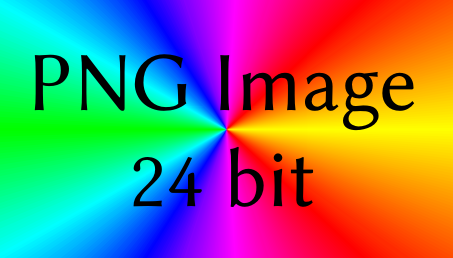
\includegraphics[width=0.4\linewidth]{images/PNG24bit.png}
   \captionof{figure}[Normale Figure Umgebung]{Dies ist eine Abbildungungsbeschriftung.}
   \label{nonfloatPNGBild24}
	\end{minipage} %Ende rechte Teilseite
	\\[\intextsep]
}

% \includegraphics[trim = 10mm 80mm 20mm 5mm, clip, width=3cm]{Bild}     %Dieser Code schneidet links 10mm, unten 80mm, rechts 20mm und oben 5mm vom urspr�nglichen Bild ab und skaliert anschliessend den sichtbaren Ausschnitt auf 3cm Breite.

% Das Bild mittels \includegraphics[bb=0 0 100 100]{Bild} ins Dokument einbinden. Die richtigen Koordinaten (ersten zwei Zahlen entsprechen der linken unteren Ecke, die zweiten zwei der rechten oberen Ecke des anzuzeigenden Bildausschnittes)

\section{Figures}
\label{sec:figures}

Als n�chstes hier mal die sehr oft anzutreffende Variante, die einer Flie�umgebung (wie es \texttt{figure} nun mal ist) das Flie�en im Text verbietet (durch \texttt{[H]} aus dem float-Paket).

An sich ist das eine normale figure Umgebung, zwei Bilder nebeneinander. Sogar gelabelt: JPEG-Bild \ref{JPEGBildN} und PNG 24-bit Bild \ref{PNGBild24}:\\
\begin{figure}[H]
   \Centering
   \begin{minipage}{0.49\linewidth}
   \Centering
   
\includegraphics[width=0.4\linewidth]{images/jpegbild_Corel24bit4,2,2.jpg}
   \caption[Normale Figure Umgebung]{Dies ist eine Abbildungungsbeschriftung.}
   \label{JPEGBildN}
	\end{minipage}%\hspace{2em}%
	\hfill%
   \begin{minipage}{0.49\linewidth}
   \Centering   
   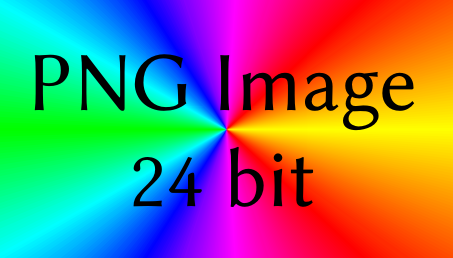
\includegraphics[width=0.4\linewidth]{images/PNG24bit.png}
   \caption[Normale Figure Umgebung]{Dies ist eine Abbildungungsbeschriftung.}
   \label{PNGBild24}
	\end{minipage}
\end{figure}

%\missingfigure{Mit dem Todo-Paket kann man sich auch an Bilder erinnern.}


\section{More figures, Subfloats, Wrapfigures}

\subsection{Overpic}

Mit dem Overpic-Paket\index{overpic} kann man LaTeX-Schrift �ber Bilder legen. Wer unbedingt will, kann so nat�rlich auch seine Grafiken beschriften, aber das Handling per Koordinaten d�rfte nicht sonderlich bequem sein. In Ausnahmef�llen kann es aber f�r eine quick-and-dirty-L�sung durchaus hilfreich sein.

Bild-�ber-Bild funktioniert genauso (siehe Beispiel, Abb.~\ref{fig:overpicex}).

\begin{figure}%
	\centering
		\begin{overpic}[scale=.25,unit=1mm]{images/PNG24bit.png}
			\put(3,28){\huge { \color{white} \LaTeX}}
			\put(40,5){
\includegraphics[scale=.07]{images/EPStoPDF_Bild.pdf}}
		\end{overpic}
\caption{Overpic-Beispiel}%
\label{fig:overpicex}%
\end{figure}




\begin{SCfigure}
\index{SCfigure}
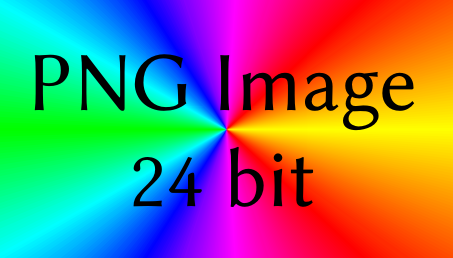
\includegraphics[width=0.4\linewidth]{images/PNG24bit.png}
   \caption[sidewayscaptionfigure]{Hier ist die Caption aber mal anders. Hier ist die Caption aber mal anders. Hier ist die Caption aber mal anders. Hier ist die Caption aber mal anders. }
   \label{fig:SCfigure}
\end{SCfigure}

Und mit Subfloats\index{subfloats} ist es �hnlich aber doch anders. Siehe \ref{fig:SCfigure} f�r eine SCfigure. Und mit Subfloats ist es �hnlich aber doch anders. N�mlich so: Wir referenzieren das gesamt-Dings mit \ref{BeidePNGBilder}, aber nur das eine mit \ref{PNGBild8S} und das andere mit \ref{PNGBild24S}. Da muss man schon im Quelltext nachschauen um das zu blicken:\\
\begin{figure}[H]
   \Centering
   \subfloat[Dies ist eine Abbildungungsbeschriftung. Erstes Bild PNG 8-bit]{\makebox[0.49\textwidth]{
\includegraphics[width=0.2\textwidth]{images/PNG8bit.png}}\label{PNGBild8S}}
      \hfill%\hspace{0.1\textwidth}
   \subfloat[Dies ist eine Abbildungungsbeschriftung. Zweites Bild PNG 24-bit]{\makebox[0.49\textwidth]{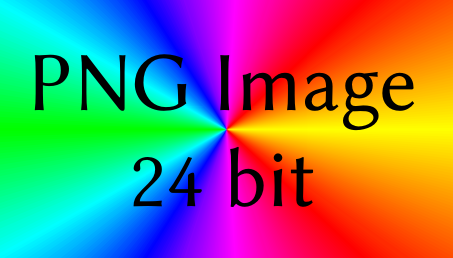
\includegraphics[width=0.2\textwidth]{images/PNG24bit.png}}\label{PNGBild24S}}
   \caption{Ein Beispiel f�r subfloats}
   \label{BeidePNGBilder}
\end{figure}

\begin{sidewaysfigure}
\Centering
   \begin{minipage}{0.49\linewidth}
   \Centering
   
\includegraphics[width=0.4\linewidth]{images/jpegbild_Corel24bit4,2,2.jpg}
   \caption[sidewaysfigure]{Geht auch quer mit \texttt{sidewaysfigure}.}
   \label{JPEGBildNQ}
	\end{minipage}%\hspace{2em}%
	\hfill%
   \begin{minipage}{0.49\linewidth}
   \Centering   
   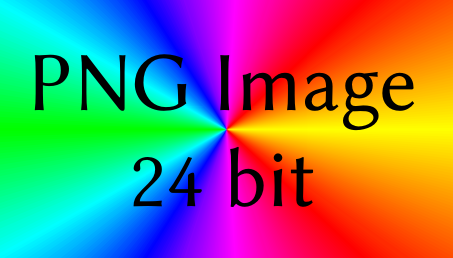
\includegraphics[width=0.4\linewidth]{images/PNG24bit.png}
   \caption[sidewaysfigure2]{Ebenso quer in derselben \texttt{sidewaysfigure}.}
   \label{PNGBild24Q}
	\end{minipage}
\end{sidewaysfigure}


Like all quotation facilities, this command is context sensitive. Depending on the nesting level, it will toggle between outer and inner quotation marks with plain and nested quotations. The starred version of this command skips directly to the inner level. If multilingual support is enabled, the style of all quotation marks will be adapted to the current language. Like all quotation facilities, this command is context sensitive. Depending on the nesting level, it will toggle between outer and inner quotation marks with plain and nested quotations. The starred version of this command skips directly to the inner level. If multilingual support is enabled, the style of all quotation marks will be adapted to the current language. Like all quotation facilities, this command is context sensitive. Depending on the nesting level, it will toggle between outer and inner quotation marks with plain and nested quotations. The starred version of this command skips directly to the inner level. If multilingual support is enabled, the style of all quotation marks will be adapted to the current language.
\section{Even more figures}
%
\includegraphics[scale=0.4]{images/PNG8bit.png}\\
%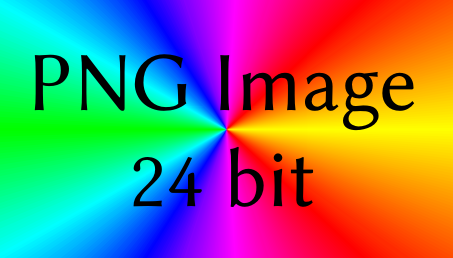
\includegraphics[scale=0.4]{images/PNG24bit.png}\\
%
\includegraphics[scale=0.4]{images/jpegbild_Corel24bit4,2,2.jpg}\\

Es ist eingestellt, dass das Gesamtdokument am Ende der PDF-Spezifikation\index{PDF-Spezifikation} 1.3 gen�gt, weil es damit keine Transparenzen aufweisen kann. Allerdings gibt das Einbetten von Dokumenten mit einer h�heren PDF-Version eine Warnung. Das ist gut, denn dann wird man daran erinnert, seine Quellgrafiken auch als Version 1.3 abzuspeichern. Wenn bei einer automatischen Konvertierung durch Zusatzpakete PDF nach Version 1.4 erzeugt wird, ist das an sich nicht schlimm, bevor man es zum Verlag in Druck gibt, kann man sich �berlegen ob man die Dateien dann h�ndisch noch per Adobe Acrobat nach PDF 1.3 konvertiert. Oft lassen sich aber auch die Zusatzoptionen bei dem Programm mit angeben. Das w�re bei \texttt{epstopdf} dann etwa \texttt{epstopdf --gsopt=-dCompatibilityLevel\#1.3 input.eps} und bei \texttt{ps2pdf} w�re das \texttt{ps2pdf -dCompatibility\#1.3 input.eps output.pdf}.

Hier ein extern nach PDF konvertiertes EPS-Bild \ref{fig:exPDFEPS}:
\begin{figure}[htb]
\Centering
\includegraphics[scale=0.4]{images/EPStoPDF_Bild.pdf}
\caption{Mit dem Programm \texttt{epstopdf.exe} konvertiertes Bild.}
\label{fig:exPDFEPS}
\end{figure}
%\includegraphics{images/nativePDF_Corel_wrongBB.pdf}\\

Normales EPS mit Includegraphics und \texttt{usepackage epstopdf}\index{epstopdf} \ref{inPDFEPS}:
\begin{figure}[htb]
%\includegraphics[scale=0.4]{images/EPSBild_Corel.eps}\hfill \includegraphics[scale=0.4]{images/psfrag_abc_def_ghi.eps}\\
\caption{Intern durch das Paket \texttt{epstopdf} on-the-fly konvertierte Bilder.}
\label{inPDFEPS}
\end{figure}


%Hier mal ein EPS als \texttt{psfragfig}. Dabei ist wichtig, die Dateiendung im Quellcode wegzulassen:\\
%\psfragfig[scale=0.5]{images/EPSBild_Corel}\\  %Warning, dass keine Macros da w�ren.
\subsection{I can't stand so much figures}

This is just english text to give an impression of running text.

Like all \index{quotation} facilities, this command is context sensitive. Depending on the nesting level, it will toggle between outer and inner quotation marks with plain and nested quotations. The starred version of this command skips directly to the inner level. If multilingual support is enabled, the style of all quotation marks will be adapted to the current language. Like all quotation facilities, this command is context sensitive. Depending on the nesting level, it will toggle between outer and inner quotation marks with plain and nested quotations. The \index{starred} version of this \index{command} skips directly to the inner level. If multilingual support is enabled, the style of all quotation marks will be adapted to the current language. Like all quotation facilities, this command is context sensitive. Depending on the nesting level, it will toggle between outer and inner quotation marks with plain and nested quotations. The starred version of this command skips directly to the inner level. If multilingual support is enabled, the style of all quotation marks will be adapted to the current language. Like all quotation facilities, this command is context sensitive. Depending on the nesting level, it will toggle between outer and inner quotation marks with plain and nested quotations. The starred version of this command skips directly to the inner level. If multilingual support is enabled, the style of all quotation marks will be adapted to the current language. Like all \index{quotation} facilities, this command is context sensitive. Depending on the nesting level, it will toggle between outer and inner quotation marks with plain and nested quotations. The starred version of this command skips directly to the inner level. If multilingual support is enabled, the style of all quotation marks will be adapted to the current language. Like all quotation facilities, this command is context sensitive. Depending on the nesting level, it will toggle between outer and inner quotation marks with plain and nested quotations. The \index{starred} version of this \index{command} skips directly to the inner level. If multilingual support is enabled, the style of all quotation marks will be adapted to the current language. Like all quotation facilities, this command is context sensitive. Depending on the nesting level, it will toggle between outer and inner quotation marks with plain and nested quotations. The starred version of this command skips directly to the inner level. If multilingual support is enabled, the style of all quotation marks will be adapted to the current language. Like all quotation facilities, this command is context sensitive. Depending on the nesting level, it will toggle between outer and inner quotation marks with plain and nested quotations. The starred version of this command skips directly to the inner level. If multilingual support is enabled, the style of all quotation marks will be adapted to the current language.

\subsubsection{Tip: Figure �ber zwei Spalten Breite}

Um Figures bei zweispaltigen Text (\zB bei einem IEEE-Paper) zu setzen, verwendet man \verb+\begin{figure*}+ und \verb+\end{figure*}+.

Das ist eher als genereller Tip zu verstehen und hat weniger mit der Vorlage zu tun.


\subsubsection{That's enough figures now}

% Wrapfloat/Wrapfigure-Hinweise:
% -The environment should be placed so as to not run over a page break.
% -The environment must not be placed in special places like lists.
% -You must not specify a wrapfigure in any type of list environment or immediately before or immediately after one.  It is OK to follow a list if there is a blank line ("\par") in between.
% -If you put a wrapfigure in a parbox or a minipage, or any other type of grouping, the text wrapping should end before the group does.
% -It may be out of sequence with regular floats.
%
% -The hlines that may be printed above and below floats are ignored; you must insert them manually if desired.
% -"\linewidth" is now adjusted within the wrapped text, but since it can only be set for whole paragraphs at a time, it will persist with the wrong value after the wrapping, until the paragraph is finished.

\index{wrapfigure}
\begin{wrapfigure}{l}{0.3\textwidth}
	\includegraphics[width=0.3\textwidth]{images/jpegbild_Corel24bit4,2,2.jpg}
	\caption{Ein Beispiel f�r wrapfigure. wrapfigure ist ein Befehl vom Paket wrapfig der ein Flie�en erlaubt. Es gibt auch wraptable f�r Tabellen.}
\end{wrapfigure}

Here is running text that is floating around figures.
Like all quotation facilities, this command is context sensitive. Depending on the nesting level, it will toggle between outer and inner quotation marks with plain and nested quotations. The starred version of this command skips directly to the inner level. If multilingual support is enabled, the style of all quotation marks will be adapted to the current language. Like all quotation facilities, this command is context sensitive. Depending on the nesting level, it will toggle between outer and inner quotation marks with plain and nested quotations. The starred version of this command skips directly to the inner level. If multilingual support is enabled, the style of all quotation marks will be adapted to the current language. Like all quotation facilities, this command is context sensitive. Depending on the nesting level, it will toggle between outer and inner quotation marks with plain and nested quotations. The starred version of this command skips directly to the inner level. If multilingual support is enabled, the style of all quotation marks will be adapted to the current language. Like all quotation facilities, this command is context sensitive. Depending on the nesting level, it will toggle between outer and inner quotation marks with plain and nested quotations. The starred version of this command skips directly to the inner level. If multilingual support is enabled, the style of all quotation marks will be adapted to the current \index{language}.

\begin{wrapfigure}[8]{r}{0.3\textwidth}  %F�r die Platzierung gibt es nicht nur r und l sondern auch i (inside) und o (outside) bei zweiseitigen Dokumenten.
	\includegraphics[width=0.3\textwidth]{images/PNG8bit.png}
	\caption{Noch ein Beispiel f�r wrapfigure. Hier wird nach 8 Zeilen der Float einfach aufgeh�rt. Es wird dann ignoriert, ob sich Text �berlagert.}
   %\vspace{-2\baselineskip}
\end{wrapfigure}

Like all quotation facilities, this command is context sensitive. Depending on the nesting level, it will toggle between outer and inner quotation marks with plain and nested quotations. The starred version of this command skips directly to the inner level. If multilingual support is enabled, the style of all quotation marks will be adapted to the current language. Like all quotation facilities, this command is context sensitive. Depending on the nesting level, it will toggle between outer and inner quotation marks with plain and nested quotations. The starred version of this command skips directly to the inner level. If multilingual support is enabled, the style of all quotation marks will be adapted to the current language. Like all quotation facilities, this command is context sensitive. Depending on the nesting level, it will toggle between outer and inner quotation marks with plain and nested quotations. The starred version of this command skips directly to the inner level. If multilingual support is enabled, the style of all quotation marks will be \index{adapted} to the current language.

\section{psfrag Bilder}

Die Basis-EPS-Dateien zur Verwendung von PSfrag\index{PSfrag} d�rfen nicht mit Inkscape 0{.}47 oder 0{.}48 gemacht werden. Inkscape 0{.}46 funktioniert hingegen.

Hintergrund ist folgender: Durch den EPS-Export per Cairo-Bibliothek in Inkscape 0{.}47 werden die Buchstaben als Einzelzeichen im EPS abgelegt. Das macht nat�rlich die Zeichenfolge insgesamt kaputt, die psfrag sucht um sie zu ersetzen. F�r Inscape 0{.}48 gibt es diesbez�glich Anpassungen, aber sie bringen das alte Verhalten nicht zur�ck sondern bringen noch die m�glichkeit eines TeX-Outputs, die aber im Falle von PSfrag nix bringt. Dieser besondere Exportmodus f�r \LaTeX tut nicht das, was f�r psfrag gebraucht wird, sondern exportiert auch per Cairo. Bleibt also erstmal nur Version 0{.}46.

Das ist mit \texttt{psfrag}-Befehlen per \texttt{pstool}\index{pstool}. Da werden die Labels aus dem Bild \ref{inPDFEPS} durch \LaTeX-Text ersetzt. Das tolle ist, dass das im Quelltext passiert und alle �nderungen an Schriften etc.\ sich dann auch sofort auf die Bilder auswirken. Bild \ref{psfragbild}:\\

% Befehle waren auskommentiert unten im pstool-Abschnitt drin

\begin{figure}[htb]
%\label{pstooltest}%
%\pstool*[%  Mit Stern hei�t: Immer processen.%
%trim= -200 0 -200 0, %
%bb = -100 0 200 0,%
%crop=pdfcrop,  %%PW: Hilft gegen falsch gecroppte BoundingBox wenn Labels drin sind %% Kann aber Fehler "Missing $" verursachen.%
%scale=0.9]{./images/psfragabcdefghiX5}{%
%				\psfrag{abc}[tc][c]{$\pi$ PStool \textbf{rocks} \textit{around}}%
%				\psfrag{def}[Bc][r][1][30]{$\frac{the}{clock}$ tonight}%
				%\psfrag{abc}[tc][c]{Ersetzung 1}%{$\pi$ PStool \textbf{rocks} \textit{around}}%
				%\psfrag{def}[Bc][r][1][30]{Ersetzung 2}%{$\frac{the}{clock}$ tonight}%
%				\psfrag{ghi}[br][r]{$e^{v\dot ery} th\cdot \jmath jng$ is gonna be alright.}%
				%\psfrag{ghi}[br][r]{Ersetzung 3}%{$e^{v\dot ery} th\cdot \jmath jng$ is gonna be alright.}%
%}
\caption{Das ist das tolle EPS aus \ref{inPDFEPS} mit \texttt{psfrag}-Ersetzungen. Hier mit dem \texttt{pstool}-Paket on-the-fly umgewandelt.}
\label{psfragbild}
\end{figure}
Bl�d ist, dass die EPS-Dateien, die Inkscape\index{Inkscape} ab Version 0.47 per Cairo erzeugt, nicht geeignet sind, weil die Labels im EPS-Quelltext nicht so abgespeichert werden, dass sie von pstool wiedergefunden werden k�nnen. Inkscape 0.46 (Export ohne Cairo) funktioniert. Ebenfalls funktioniert der EPS-Export von CorelDraw X4.

Im Quelltext ist hier \texttt{pstool*} zu finden statt nur \texttt{pstool}. Das bedeutet, dass die Grafiken jedes mal neu erzeugt werden. Das ist gut f�r Debugging-Zwecke, aber \textbf{verl�ngert die Kompilierzeit erheblich}! Wer also immer drandenkt wenn er seine Grafiken aktualisiert und wieder mal scheinbar nix passiert, kann das Sternchen getrost wegmachen.

%Das ist mittels \texttt{psfrag}-Befehlen:
%\begin{minipage}{\textwidth}
%\label{psfragtest}
%        \psfrag{abc}[c][c]{$\pi$ Rock around}
%        \psfrag{def}[c][c]{$\frac{the}{clock}$ tonight}
%        \psfrag{ghi}[c][c]{$e^{v\dot ery}th\dot \i ng$ is gonna be alright.}
%        \includegraphics[scale=0.4,trim= -20 0 -20 0]{images/psfrag_abc_def_ghi.eps}
%       
%\end{minipage}


%\psfrag{tag}[posn][psposn][scale][rot]{LATEX text}
%[posn] the LATEX text reference point. The syntax of this argument is identical to that of the \makebox command. Up to two letters may be chosen, one from the list {t,b,B,c}, (top, bottom, baseline, center) and another from {l,r,c} (left, right, center). If either letter is omitted, then c (center) is assumed. Together, these specify one of 12 anchor points. If the argument is omitted altogether, then [Bl], or left baseline positioning, is assumed�but note that supplying [] specifies centered positioning. When running in LATEX 2.09 compatibility mode, the default alignment is [bl], in order to support legacy documents. Usually this should not make a significant difference.
%[psposn] the PostScript text reference point. The possible arguments are identical to that of [posn], as is the default value, [Bl] ([bl] in LATEX 2.09 compatibility mode.)

\section{Matlab-Bilder und Mathematica-Bilder}
\label{sec:matlabbilder}
Die Vorlage bietet Unterst�tzung f�r Bilder aus Matlab\index{Matlab} und Mathematica\index{Mathematica}: Mithilfe des \verb+\psfragfig+-Befehls aus dem \texttt{pstool}-Paket k�nnen Bilder eingef�gt werden, die mit \texttt{matlabfrag}\footnote{\url{http://www.mathworks.com/matlabcentral/fileexchange/21286-matlabfrag}}\index{matlabfrag} (Matlab) bzw.\ \texttt{MathPSfrag}\footnote{\url{http://wwwth.mppmu.mpg.de/members/jgrosse/mathpsfrag/}} (Mathematica) erstellt wurden. Diese erhalten dann auch die Beschriftung durch \LaTeX, d.h. man kann auch \LaTeX-Code in die Beschriftung in Matlab schreiben und sp�ter sieht es richtig aus.

Beispiel sind Bild \ref{Matlabscreen}, \ref{matlabfragbild1} und \ref{matlabfragbild2}.

\begin{figure}[htb]
	\Centering
	\includegraphics[scale=0.4]{images/matlabfrag/matlabfrag_matlab.png}
	\caption{So sieht's in Matlab aus.}
	\label{Matlabscreen}
\end{figure}

\begin{figure}[htb]
	\Centering
%	\psfragfig*[%
	%crop=pdfcrop,  %%PW: Hilft gegen falsch gecroppte BoundingBox wenn Labels drin sind %% Kann aber Fehler "Missing $" verursachen.
%	scale=0.4]{./images/matlabfrag/ex01-1}
%	{
%	% Generated using matlabfrag
% Version: v0.6.16
% Version Date: 04-Apr-2010
% Author: Zebb Prime
%
%% <text>
%
\providecommand\matlabtextA{\color[rgb]{0.000,0.000,0.000}\fontsize{10}{10}\selectfont\strut}%
\psfrag{022}[tl][tl]{\matlabtextA $\int\limits_{a_k}^{b^w}{d\cdot r \partial x}$}%
\psfrag{023}[cc][cc]{\matlabtextA Textpfeil}%
\psfrag{024}[tl][tl]{\matlabtextA \begin{tabular}{@{}l@{}}Pfeil auf bunte Linie\\Text in zwei Linien\end{tabular}}%
%
%% </text>
%
%% <xtick>
%
\def\matlabfragNegXTick{\mathord{\makebox[0pt][r]{$-$}}}
%
\psfrag{000}[ct][ct]{\matlabtextA $1$}%
\psfrag{001}[ct][ct]{\matlabtextA $1.1$}%
\psfrag{002}[ct][ct]{\matlabtextA $1.2$}%
\psfrag{003}[ct][ct]{\matlabtextA $1.3$}%
\psfrag{004}[ct][ct]{\matlabtextA $1.4$}%
\psfrag{005}[ct][ct]{\matlabtextA $1.5$}%
\psfrag{006}[ct][ct]{\matlabtextA $1.6$}%
\psfrag{007}[ct][ct]{\matlabtextA $1.7$}%
\psfrag{008}[ct][ct]{\matlabtextA $1.8$}%
\psfrag{009}[ct][ct]{\matlabtextA $1.9$}%
\psfrag{010}[ct][ct]{\matlabtextA $2$}%
%
%% </xtick>
%
%% <ytick>
%
\psfrag{011}[rc][rc]{\matlabtextA $0$}%
\psfrag{012}[rc][rc]{\matlabtextA $0.1$}%
\psfrag{013}[rc][rc]{\matlabtextA $0.2$}%
\psfrag{014}[rc][rc]{\matlabtextA $0.3$}%
\psfrag{015}[rc][rc]{\matlabtextA $0.4$}%
\psfrag{016}[rc][rc]{\matlabtextA $0.5$}%
\psfrag{017}[rc][rc]{\matlabtextA $0.6$}%
\psfrag{018}[rc][rc]{\matlabtextA $0.7$}%
\psfrag{019}[rc][rc]{\matlabtextA $0.8$}%
\psfrag{020}[rc][rc]{\matlabtextA $0.9$}%
\psfrag{021}[rc][rc]{\matlabtextA $1$}%
%
%% </ytick>
%	}
	\caption{Matlabfragbild Nummer 1}
	\label{matlabfragbild1}
\end{figure}

\begin{figure}[htb]
	\Centering
%	\psfragfig*[%
	%crop=pdfcrop,  %%PW: Hilft gegen falsch gecroppte BoundingBox wenn Labels drin sind %% Kann aber Fehler "Missing $" verursachen.
%	scale=0.4]{./images/matlabfrag/ex01-2}{%
%	% Generated using matlabfrag
% Version: v0.6.16
% Version Date: 04-Apr-2010
% Author: Zebb Prime
%
%% <text>
%
\providecommand\matlabtextA{\color[rgb]{0.000,0.000,0.000}\fontsize{10}{10}\selectfont\strut}%
\psfrag{022}[tl][tl]{\matlabtextA $\int\limits_{a_k}^{b^w}{d\cdot r \partial x}$}%
\psfrag{023}[cc][cc]{\matlabtextA Textpfeil}%
\psfrag{024}[tl][tl]{\matlabtextA \begin{tabular}{@{}l@{}}Pfeil auf bunte Linie\\Text in zwei Linien\end{tabular}}%
%
%% </text>
%
%% <xtick>
%
\def\matlabfragNegXTick{\mathord{\makebox[0pt][r]{$-$}}}
%
\psfrag{000}[ct][ct]{\matlabtextA $1$}%
\psfrag{001}[ct][ct]{\matlabtextA $1.1$}%
\psfrag{002}[ct][ct]{\matlabtextA $1.2$}%
\psfrag{003}[ct][ct]{\matlabtextA $1.3$}%
\psfrag{004}[ct][ct]{\matlabtextA $1.4$}%
\psfrag{005}[ct][ct]{\matlabtextA $1.5$}%
\psfrag{006}[ct][ct]{\matlabtextA $1.6$}%
\psfrag{007}[ct][ct]{\matlabtextA $1.7$}%
\psfrag{008}[ct][ct]{\matlabtextA $1.8$}%
\psfrag{009}[ct][ct]{\matlabtextA $1.9$}%
\psfrag{010}[ct][ct]{\matlabtextA $2$}%
%
%% </xtick>
%
%% <ytick>
%
\psfrag{011}[rc][rc]{\matlabtextA $0$}%
\psfrag{012}[rc][rc]{\matlabtextA $0.1$}%
\psfrag{013}[rc][rc]{\matlabtextA $0.2$}%
\psfrag{014}[rc][rc]{\matlabtextA $0.3$}%
\psfrag{015}[rc][rc]{\matlabtextA $0.4$}%
\psfrag{016}[rc][rc]{\matlabtextA $0.5$}%
\psfrag{017}[rc][rc]{\matlabtextA $0.6$}%
\psfrag{018}[rc][rc]{\matlabtextA $0.7$}%
\psfrag{019}[rc][rc]{\matlabtextA $0.8$}%
\psfrag{020}[rc][rc]{\matlabtextA $0.9$}%
\psfrag{021}[rc][rc]{\matlabtextA $1$}%
%
%% </ytick>
%	}
	\caption{Matlabfragbild Nummer 2. Gleicher Inhalt, aber andere EPS-BoundingBox.}
	\label{matlabfragbild2}
\end{figure}


\subsection{Matlab und TikZ}

Wer Matlab lieber mit TikZ\index{TikZ} statt mit PSfrag verheiraten m�chte, dem seien diese Projekte ans Herz gelegt:

matlab2tikz\\
\url{http://www.mathworks.com/matlabcentral/fileexchange/22022}

Matfig2PGF\\
\url{http://www.mathworks.com/matlabcentral/fileexchange/12962}

\section{TikZ-Bilder}

Eine sehr gro�e Auswahl, was man mit TikZ\index{TikZ} machen kann und wie es geht (Quellcode dazu!!) findet man bei den \TeX amples:

\url{http://www.texample.net/tikz/examples/all}

Das polarisierende Mikroskop aus den \TeX amples ist unter Abb.~\ref{fig:tikzpolarizingmicroscope} zu sehen. Die Originaldatei verwendet jedoch den Befehl \texttt{opacity}. \textbf{Achtung}: Dieser Befehl erzeugt Transparenzen, die beim Druck durch KIT SP nicht erw�nscht sind! Also auch bei TikZ aufpassen.

Jetzt kommt ein tolles \textbf{\texttt{TikZ}}-Bild mit \texttt{TikZ} in Abb.~\ref{fig:tikzkalmanfilterdiagram}. Es zeigt ein h�bsches Kalmanfilter aus den \TeX amples:

%%PW: TikZ-Beispiele hier: http://www.texample.net/tikz/examples/ zum runterladen
\begin{figure}[htb]
%	% Polarizing microscope
% Author: Cyril Langlois
% This TikZ code sketches the light behavior during its travel in a polarizing
% petrographic microscope when a birefringent crystal thin section is inserted
% between the polarizing devices.
% 
% The goal was to correctly show the vectorial relationships between light
% electric fields during its travel through the first polaroid, the mineral
% section and the second polaroid.


\begin{tikzpicture}[x={(0.866cm,-0.5cm)}, y={(0.866cm,0.5cm)}, z={(0cm,1cm)}, scale=0.5,
    %Option for nice arrows
    >=stealth, %
	  inner sep=0pt, outer sep=2pt,%
    axis/.style={thick,->},
    wave/.style={thick,color=#1,smooth},
    polaroid/.style={fill=black!60!white}%, opacity=0.3},
]
    % Colors
    \colorlet{darkgreen}{green!50!black}
    \colorlet{lightgreen}{green!80!black}
    \colorlet{darkred}{red!50!black}
    \colorlet{lightred}{red!80!black}

    % Frame
    \coordinate (O) at (0, 0, 0);
    \draw[axis] (O) -- +(14, 0,   0) node [right] {x};
    \draw[axis] (O) -- +(0,  2.5, 0) node [right] {y};
    \draw[axis] (O) -- +(0,  0,   2) node [above] {z};

    \draw[thick,dashed] (-2,0,0) -- (O);

    % monochromatic incident light with electric field
    \draw[wave=blue, variable=\x, samples at={-2,-1.75,...,0}]%opacity=0.7,
        plot (\x, { cos(1.0*\x r)*sin(2.0*\x r)}, { sin(1.0*\x r)*sin(2.0*\x r)})
        plot (\x, {-cos(1.0*\x r)*sin(2.0*\x r)}, {-sin(1.0*\x r)*sin(2.0*\x r)});

    \foreach \x in{-2,-1.75,...,0}{
        \draw[color=blue, ->] %opacity=0.7,
            (\x,0,0) -- (\x, { cos(1.0*\x r)*sin(2.0*\x r)}, { sin(1.0*\x r)*sin(2.0*\x r)})
            (\x,0,0) -- (\x, {-cos(1.0*\x r)*sin(2.0*\x r)}, {-sin(1.0*\x r)*sin(2.0*\x r)});
    }

    \filldraw[polaroid] (0,-2,-1.5) -- (0,-2,1.5) -- (0,2,1.5) -- (0,2,-1.5) -- (0,-2,-1.5)
        node[below, sloped, near end]{Polaroid};%

    %Direction of polarization
    \draw[thick,<->] (0,-1.75,-1) -- (0,-0.75,-1);

    % Electric field vectors
    \draw[wave=blue, variable=\x,samples at={0,0.25,...,6}]
        plot (\x,{sin(2*\x r)},0)node[anchor=north]{$\vec{E}$};

    %Polarized light between polaroid and thin section
    \foreach \x in{0, 0.25,...,6}
        \draw[color=blue,->] (\x,0,0) -- (\x,{sin(2*\x r)},0);

    \draw (3,1,1) node [text width=2.5cm, text centered]{Polarized light};

    %Crystal thin section
    \begin{scope}[thick]
        \draw (6,-2,-1.5) -- (6,-2,1.5) node [above, sloped, midway]{Crystal section}
                -- (6, 2, 1.5) -- (6, 2, -1.5) -- cycle % First face
            (6,  -2, -1.5) -- (6.2, -2,-1.5)
            (6,   2, -1.5) -- (6.2,  2,-1.5)
            (6,  -2,  1.5) -- (6.2, -2, 1.5)
            (6,   2,  1.5) -- (6.2,  2, 1.5)
            (6.2,-2, -1.5) -- (6.2, -2, 1.5) -- (6.2, 2, 1.5) 
                -- (6.2, 2, -1.5) -- cycle; % Second face

        %Optical indices
        \draw[darkred, ->]       (6.1, 0, 0) -- (6.1, 0.26,  0.966) node [right] {$n_{g}'$}; % index 1
        \draw[darkred, dashed]   (6.1, 0, 0) -- (6.1,-0.26, -0.966); % index 1
        \draw[darkgreen, ->]     (6.1, 0, 0) -- (6.1, 0.644,-0.173) node [right] {$n_{p}'$}; % index 2
        \draw[darkgreen, dashed] (6.1, 0, 0) -- (6.1,-0.644, 0.173); % index 2
    \end{scope}

    %Rays leaving thin section
    \draw[wave=darkred,   variable=\x, samples at={6.2,6.45,...,12}] 
        plot (\x, {0.26*0.26*sin(2*(\x-0.5) r)},  {0.966*0.26*sin(2*(\x-0.5) r)});  %n'g-oriented ray
    \draw[wave=darkgreen, variable=\x, samples at={6.2,6.45,...,12}]
        plot (\x, {0.966*0.966*sin(2*(\x-0.1) r)},{-0.26*0.966*sin(2*(\x-0.1) r)}); %n'p-oriented ray
    \draw (10,1,1) node [text width=2.5cm, text centered] {Polarized and dephased light};

    \foreach \x in{6.2,6.45,...,12} {
        \draw[color=darkgreen, ->] (\x, 0, 0) --
            (\x, {0.966*0.966*sin(2*(\x-0.1) r)}, {-0.26*0.966*sin(2*(\x-0.1) r)});
        \draw[color=darkred,   ->] (\x, 0, 0) --
            (\x, {0.26*0.26*sin(2*(\x-0.5) r)}, {0.966*0.26*sin(2*(\x-0.5) r)});
    }

    %Second polarization
    \draw[polaroid]   (12, -2,  -1.5) -- (12, -2,   1.5)  %Polarizing filter
        node [above, sloped,midway] {Polaroid} -- (12, 2, 1.5) -- (12, 2, -1.5) -- cycle;
    \draw[thick, <->] (12, -1.5,-0.5) -- (12, -1.5, 0.5); %Polarization direction

    %Light leaving the second polaroid
    \draw[wave=lightgreen,variable=\x, samples at={12, 12.25,..., 14}]
        plot (\x,{0}, {0.966*0.966*0.26*sin(2*(\x-0.5) r)}); %n'g polarized ray
    \draw[wave=lightred,  variable=\x, samples at={12, 12.25,..., 14}]
        plot (\x,{0}, {-0.26*0.966*sin(2*(\x-0.1) r)});      %n'p polarized ray

    \node[text width=14cm, anchor=north west, yshift=-2mm] at (current bounding box.south west)
        {Light behavior in a petrographic microscope with light polarizing
        device. Only one incident wavelength is shown (monochromatic light).
        The magnetic field, perpendicular to the electric one, is not drawn.};
\end{tikzpicture}

\caption[Polarisiertes Licht]{TikZ-Bild polarisiertes Licht. Der obige Text steht seltsamerweise im TikZ-Bild drin. Das ist nicht gut, weil bei �nderungen des Papierformats der Text nur noch schlecht aussieht.}
\label{fig:tikzpolarizingmicroscope}
\end{figure}

\begin{figure}[htbp]%
%	
\centering%
% The state vector is represented by a blue circle.
% "minimum size" makes sure all circles have the same size
% independently of their contents.
\tikzstyle{state}=[circle,
                                    thick,
                                    minimum size=1.1cm,
                                    draw=blue!80,
                                    fill=blue!20]

% The measurement vector is represented by an orange circle.
\tikzstyle{measurement}=[circle,
                                                thick,
                                                minimum size=1.1cm,
                                                draw=orange!80,
                                                fill=orange!25]

% The control input vector is represented by a purple circle.
\tikzstyle{input}=[circle,
                                    thick,
                                    minimum size=1.1cm,
                                    draw=purple!80,
                                    fill=purple!20]

% The input, state transition, and measurement matrices
% are represented by gray squares.
% They have a smaller minimal size for aesthetic reasons.
\tikzstyle{matrx}=[rectangle,
                                    thick,
                                    minimum size=0.9cm,
                                    draw=gray!80,
                                    fill=gray!20]

% The system and measurement noise are represented by yellow
% circles with a "noisy" uneven circumference.
% This requires the TikZ library "decorations.pathmorphing".
\tikzstyle{noise}=[circle,
                                    thick,
                                    minimum size=1.1cm,
                                    draw=yellow!85!black,
                                    fill=yellow!40,
                                    decorate,
                                    decoration={random steps,
                                                            segment length=2pt,
                                                            amplitude=2pt}]

% Everything is drawn on underlying gray rectangles with
% rounded corners.
\tikzstyle{background}=[rectangle,
                                                fill=gray!10,
                                                inner sep=0.1cm,
                                                rounded corners=4mm]
\begin{tikzpicture}[>=latex,text height=1.5ex,text depth=0.25ex]%
    % "text height" and "text depth" are required to vertically
    % align the labels with and without indices.
  % The various elements are conveniently placed using a matrix:
  \matrix[row sep=0.3cm,column sep=0.3cm] {%
    % First line: Control input
    &%
        \node (u_k-1) [input]{$\mathbf{u}_{k-1}$}; &%
        &%
        \node (u_k)   [input]{$\mathbf{u}_k$};     &%
        &%
        \node (u_k+1) [input]{$\mathbf{u}_{k+1}$}; &%
        \\%
        % Second line: System noise & input matrix
        \node (w_k-1) [noise] {$\mathbf{w}_{k-1}$}; &%
        \node (B_k-1) [matrx] {$\mathbf{B}$};       &%
        \node (w_k)   [noise] {$\mathbf{w}_k$};     &%
        \node (B_k)   [matrx] {$\mathbf{B}$};       &%
        \node (w_k+1) [noise] {$\mathbf{w}_{k+1}$}; &%
        \node (B_k+1) [matrx] {$\mathbf{B}$};       &%
        \\%
        % Third line: State & state transition matrix
        \node (A_k-2)         {$\cdots$};           &%
        \node (x_k-1) [state] {$\mathbf{x}_{k-1}$}; &%
        \node (A_k-1) [matrx] {$\mathbf{A}$};       &%
        \node (x_k)   [state] {$\mathbf{x}_k$};     &%
        \node (A_k)   [matrx] {$\mathbf{A}$};       &%
        \node (x_k+1) [state] {$\mathbf{x}_{k+1}$}; &%
        \node (A_k+1)         {$\cdots$};           \\%
        % Fourth line: Measurement noise & measurement matrix
        \node (v_k-1) [noise] {$\mathbf{v}_{k-1}$}; &%
        \node (H_k-1) [matrx] {$\mathbf{H}$};       &%
				\node (v_k)   [noise] {$\mathbf{v}_k$};     &%
        \node (H_k)   [matrx] {$\mathbf{H}$};       &%
        \node (v_k+1) [noise] {$\mathbf{v}_{k+1}$}; &%
        \node (H_k+1) [matrx] {$\mathbf{H}$};       &%
        \\%
        % Fifth line: Measurement
        & \node (z_k-1) [measurement] {$\mathbf{z}_{k-1}$};
				&%
        & \node (z_k)   [measurement] {$\mathbf{z}_k$};
				&%
        & \node (z_k+1) [measurement] {$\mathbf{z}_{k+1}$};
				&%
        \\%
    };%
    % The diagram elements are now connected through arrows:
    \path[->]%
        (A_k-2) edge[thick] (x_k-1)	% The main path between the
        (x_k-1) edge[thick] (A_k-1)	% states via the state
        (A_k-1) edge[thick] (x_k)		% transition matrices is
        (x_k)   edge[thick] (A_k)		% accentuated.
        (A_k)   edge[thick] (x_k+1)	% x -> A -> x -> A -> ...
        (x_k+1) edge[thick] (A_k+1)%%%%
        (x_k-1) edge (H_k-1)				% Output path x -> H -> z
        (H_k-1) edge (z_k-1)%
        (x_k)   edge (H_k)%
        (H_k)   edge (z_k)%
        (x_k+1) edge (H_k+1)%
        (H_k+1) edge (z_k+1)%%%%%
        (v_k-1) edge (z_k-1)				% Output noise v -> z
        (v_k)   edge (z_k)%
        (v_k+1) edge (z_k+1)%%%
        (w_k-1) edge (x_k-1)				% System noise w -> x
        (w_k)   edge (x_k)%
        (w_k+1) edge (x_k+1)%%%%
        (u_k-1) edge (B_k-1)				% Input path u -> B -> x
        (B_k-1) edge (x_k-1)%
        (u_k)   edge (B_k)%
        (B_k)   edge (x_k)%
        (u_k+1) edge (B_k+1)%
        (B_k+1) edge (x_k+1)%
        ;%
    % Now that the diagram has been drawn, background rectangles
    % can be fitted to its elements. This requires the TikZ
    % libraries "fit" and "background".
    % Control input and measurement are labeled. These labels have
    % not been translated to English as "Measurement" instead of
    % "Messung" would not look good due to it being too long a word.
    \begin{pgfonlayer}{background}%
        \node [background,%
                    fit=(u_k-1) (u_k+1),%
                    label=left:Input:] {};%
        \node [background,%
                    fit=(z_k-1) (z_k+1),%
                    label=left:Measure:] {};%
				\node [background,%
				fit=(w_k-1) (v_k-1) (A_k+1)] {};%
    \end{pgfonlayer}%
\end{tikzpicture}%

\caption[Shortened for TOC: System model of the (linear) Kalman filter.]{This is the system model of the (linear) Kalman filter. At each time step the state vector $\mathbf{x}_k$ is propagated to the new state
estimation $\mathbf{x}_{k+1}$ by multiplication with the constant state transition matrix $\mathbf{A}$. The state vector $\mathbf{x}_{k+1}$ is additionally influenced by the control input vector $\mathbf{u}_{k+1}$ multiplied by the input matrix $\mathbf{B}$, and the system noise vector $\mathbf{w}_{k+1}$. The system state cannot be measured directly. The measurement vector $\mathbf{z}_k$ consists of the information contained within the state vector $\mathbf{x}_k$ multiplied by the measurement matrix $\mathbf{H}$, and the additional measurement noise $\mathbf{v}_k$.}
\label{fig:tikzkalmanfilterdiagram}
\end{figure}%


\subsection{3D-Grafiken und TikZ}

Ein Paket zur einfacheren Erstellung von 3D-Grafiken ist \texttt{Sketch}. Sketch ist praktisch eine 3D-Programmiersprache, die Output in PSTricks oder TikZ\index{TikZ} generiert.
\url{http://www.frontiernet.net/~eugene.ressler/}

Ein etwas weniger gro�es Framework (und damit m�glicherweise einfacher zu lernen) ist das Package \texttt{tikz-3dplot}.
Wenn es nicht um Oberfl�chenmodellierung geht, reicht evtl.\ auch das, siehe Figure~\ref{fig:tikz3d}.

\begin{figure}[htb]
	\Centering
%%% Copyright 2009 Jeffrey D. Hein
%
% This work may be distributed and/or modified under the
% conditions of the LaTeX Project Public License, either version 1.3
% of this license or (at your option) any later version.
% The latest version of this license is in
%   http://www.latex-project.org/lppl.txt
% and version 1.3 or later is part of all distributions of LaTeX
% version 2005/12/01 or later.
%
% This work has the LPPL maintenance status `maintained'.
% 
% The Current Maintainer of this work is Jeffrey D. Hein.
%
% This work consists of the files 3dplot.sty and 3dplot.tex

%Description
%-----------
%3dplot.tex - an example file demonstrating the use of the 3dplot.sty package.

%-----------------

%set the plot display orientation
%synatax: \tdplotsetdisplay{\theta_d}{\phi_d}
\tdplotsetmaincoords{60}{110}

%define polar coordinates for some vector
%TODO: look into using 3d spherical coordinate system
\pgfmathsetmacro{\rvec}{.8}
\pgfmathsetmacro{\thetavec}{30}
\pgfmathsetmacro{\phivec}{60}

%start tikz picture, and use the tdplot_main_coords style to implement the display 
%coordinate transformation provided by 3dplot
\begin{tikzpicture}[scale=5,tdplot_main_coords]

%set up some coordinates 
%-----------------------
\coordinate (O) at (0,0,0);

%determine a coordinate (P) using (r,\theta,\phi) coordinates.  This command
%also determines (Pxy), (Pxz), and (Pyz): the xy-, xz-, and yz-projections
%of the point (P).
%syntax: \tdplotsetcoord{Coordinate name without parentheses}{r}{\theta}{\phi}
\tdplotsetcoord{P}{\rvec}{\thetavec}{\phivec}

%draw figure contents
%--------------------

%draw the main coordinate system axes
\draw[thick,->] (0,0,0) -- (1,0,0) node[anchor=north east]{$x$};
\draw[thick,->] (0,0,0) -- (0,1,0) node[anchor=north west]{$y$};
\draw[thick,->] (0,0,0) -- (0,0,1) node[anchor=south]{$z$};

%draw a vector from origin to point (P) 
\draw[-stealth,color=red] (O) -- (P);

%draw projection on xy plane, and a connecting line
\draw[dashed, color=red] (O) -- (Pxy);
\draw[dashed, color=red] (P) -- (Pxy);

%draw the angle \phi, and label it
%syntax: \tdplotdrawarc[coordinate frame, draw options]{center point}{r}{angle}{label options}{label}
\tdplotdrawarc{(O)}{0.2}{0}{\phivec}{anchor=north}{$\phi$}


%set the rotated coordinate system so the x'-y' plane lies within the
%"theta plane" of the main coordinate system
%syntax: \tdplotsetthetaplanecoords{\phi}
\tdplotsetthetaplanecoords{\phivec}

%draw theta arc and label, using rotated coordinate system
\tdplotdrawarc[tdplot_rotated_coords]{(0,0,0)}{0.5}{0}{\thetavec}{anchor=south west}{$\theta$}

%draw some dashed arcs, demonstrating direct arc drawing
\draw[dashed,tdplot_rotated_coords] (\rvec,0,0) arc (0:90:\rvec);
\draw[dashed] (\rvec,0,0) arc (0:90:\rvec);

%set the rotated coordinate definition within display using a translation
%coordinate and Euler angles in the "z(\alpha)y(\beta)z(\gamma)" euler rotation convention
%syntax: \tdplotsetrotatedcoords{\alpha}{\beta}{\gamma}
\tdplotsetrotatedcoords{\phivec}{\thetavec}{0}

%translate the rotated coordinate system
%syntax: \tdplotsetrotatedcoordsorigin{point}
\tdplotsetrotatedcoordsorigin{(P)}

%use the tdplot_rotated_coords style to work in the rotated, translated coordinate frame
\draw[thick,tdplot_rotated_coords,->] (0,0,0) -- (.5,0,0) node[anchor=north west]{$x'$};
\draw[thick,tdplot_rotated_coords,->] (0,0,0) -- (0,.5,0) node[anchor=west]{$y'$};
\draw[thick,tdplot_rotated_coords,->] (0,0,0) -- (0,0,.5) node[anchor=south]{$z'$};

%WARNING:  coordinates defined by the \coordinate command (eg. (O), (P), etc.)
%cannot be used in rotated coordinate frames.  Use only literal coordinates.  

%draw some vector, and its projection, in the rotated coordinate frame
\draw[-stealth,color=blue,tdplot_rotated_coords] (0,0,0) -- (.2,.2,.2);
\draw[dashed,color=blue,tdplot_rotated_coords] (0,0,0) -- (.2,.2,0);
\draw[dashed,color=blue,tdplot_rotated_coords] (.2,.2,0) -- (.2,.2,.2);

%show its phi arc and label
\tdplotdrawarc[tdplot_rotated_coords,color=blue]{(0,0,0)}{0.2}{0}{45}{anchor=north west,color=black}{$\phi'$}

%change the rotated coordinate frame so that it lies in its theta plane.
%Note that this overwrites the original rotated coordinate frame
%syntax: \tdplotsetrotatedthetaplanecoords{\phi'}
\tdplotsetrotatedthetaplanecoords{45}

%draw theta arc and label
\tdplotdrawarc[tdplot_rotated_coords,color=blue]{(0,0,0)}{0.2}{0}{55}{anchor=south west,color=black}{$\theta'$}

\end{tikzpicture}


\caption{Bild erstellt mit tikz-3dplot.}
\label{fig:tikz3d}
\end{figure}


\section{Bilder mit Asymptote}
\label{sec:asy}
Ist nicht so einfach, geht auch nur holprig.

Zuerst muss man Asymptote\index{Asymptote} runterladen\footnote{\url{http://asymptote.sourceforge.net/}} und installieren. Au�erdem muss (wie schon am Anfang empfohlen) ein aktuelles Ghostscript installiert sein. Im Folgenden wird erwartet, dass der geneigte Leser die Transferleistung erbringt, die Pfade an sein System anzupassen \Smiley.

Dann einen Ordner namens \texttt{asymptote} im Verzeichnis \\ \verb+c:\Programme\MiKTeX28\tex\latex\+ anlegen und die \texttt{asycolors.sty} sowie die \texttt{asymptote.sty} reinkopieren.

Anschlie�end muss man Mik\TeX noch die Dateien in den internen Index aufnehmen lassen, dass sie als bekannt gelten. Dazu unter Mik\TeX, Maintenance (Admin), Settings (Admin) auf \enquote{Refresh FNDB} (Filename Database) klicken. Ab dann kennt Mik\TeX das Paket und man kann \verb+\usepackage{asymptote}+ verwenden.

Allerdings geschieht die Erzeugung noch nicht vollautomatisch. Das Bild \ref{fig:asyimage} war urspr�nglich ein inline-Bild (Asy-Code im \LaTeX-Code), allerdings ist es jetzt als normales PDF eingebunden (Grund s{.}\,u{.}). Da wird nach dem ersten pdf\LaTeX-Lauf eine \texttt{<haupttexdateiname>-1.asy} erzeugt. Die muss man per Doppelklick ausf�hren (dabei wird ein PDF und ein Hilfs-\LaTeX-Dokument erzeugt) und beim n�chsten pdf\LaTeX-Lauf erscheint dann das Bild. Problem ist hierbei aber noch, dass man noch eine Umgebungsvariable (Benutzer-Umgebungsvariable reicht) namens \texttt{ASYMPTOTE\_GS} mit dem Wert \\ \verb+c:\Programme\Ghostscript\gs8.71\bin\gswin32c.exe+ (f�r Ghostscript v8{.}71) setzen muss und Gr��en�nderungen so nicht direkt vorgesehen sind.

\begin{figure}%
\Centering
	\includegraphics[width=0.2\textwidth]{images/asymptote/asymptoteexamplepdf13.pdf}%
	\caption{Ergebnis des Asymptote-Inlinebilds}%
	\label{fig:asyimage}%
\end{figure}

%% Inline-Code mit dem das Bild erzeugt wurde. Zur Vermeidung der \write-Problematik wird aber Asymptote wieder rausgeworfen und comment eingesetzt.
%\begin{asy}
	%include graph;
	%size(1inch);
	%filldraw(circle((0,0),1),yellow,black);
	%fill(circle((-.3,.4),.1),black);
	%fill(circle((.3,.4),.1),black);
	%draw(arc((0,0),.5,-140,-40));
%\end{asy}

Leider ist die Integration alles andere als nahtlos. Auch Beispiele aus der Asymptote-Gallery funktionieren nicht so, wie sie sollen. Am einfachsten ist es wahrscheinlich, die Asymptote-Grafiken separat als PDF zu erzeugen und normal als Bild einzubinden. Dies geschieht durch aufruf von \texttt{asy -f pdf <asyfile.asy>} bzw.\ \texttt{asy -tex pdflatex <asyfile.asy>}. Allerdings muss man dann darauf achten, dass man die \LaTeX-Schrift f�rs Bild korrekt w�hlt (im wesentlichen das Paket \texttt{fourier}, aber bei anderen Mathezeichen wirds dann kompliziert). Deshalb muss in der Asymptote-Datei noch folgendes eingef�gt werden:\\
\begin{verbatim}
\usepackage("fourier");
defaultpen(font("T1","fut\textfamilyextension","m","n"));
\end{verbatim}

Die technische Begr�ndung f�r diese Unannehmlichkeiten: Asymptote braucht auch ein \TeX-\verb+\write+, von denen es nur 16 gibt (\TeX\ ist halt ewig alt). Man hat also die Wahl zwischen \zb \texttt{comment} und \texttt{asymptote}. Um das comment-Paket demonstieren zu k�nnen, wurde obige Inline-Grafik als PDF eingef�gt. Vermutlich ist es generell einfacher, Asymptote-Grafiken auf diese Weise einzuf�gen.

%\asyfig{images/asymptote/helix}


%\newcommand{\welcome}{Welcome!}
%\begin{figure}
%\Centering
%\begin{asy}
%size (3cm, 0);
%label (Label ("\welcome", "Welcome!"), (0,0));
%shipout(bbox(0.5cm));
%\end{asy}
%\caption{Correct bounding box.}
%\end{figure}
%
%\begin{figure}[htb]
	%\Centering
  %\includegraphics[width=\linewidth]{images/asymptote/helix}
  %\caption{This is a margin figure.  The helix is defined by 
    %$x = \cos(2\pi z)$, $y = \sin(2\pi z)$, and $z = [0, 2.7]$.  The figure was
    %drawn using Asymptote\footnote{\url{http://asymptote.sf.net/}}.}
  %\label{fig:marginfig} 
%\end{figure}

\section{3D-Bilder und Videos}
Seit PDF-Version 1{.}6 (Acrobat 7{.}0, 2005) sind 3D-Objekte in PDFs\index{3D im PDF} m�glich. Diese k�nnen \zb im PRC-Format durch \texttt{asy -inlineimage -tex pdflatex <asyfile.asy>} mit Asymptote erzeugt und mithilfe des \texttt{movie15}-Pakets eingef�gt werden. In der Druckversion f�r die KIT-Druckerei d�rfen aber sowieso keine 3D-Elemente im PDF vorhanden sein wegen der angestrebten PDF/A-Kompatibilit�t. SumatraPDF scheint au�erdem keine Unterst�tzung f�r 3D in PDF mitzubringen. Will man die Elemente f�r Online-Publishing drinhaben, sollte man auch daran denken, dass der pdfminorversion-Befehl die PDF-Version nach oben beschr�nkt und das entsprechend �ndern.

% Movie15-Test
%\begin{figure}%
	%\Centering%
	%\includemovie[label=fig:3dimage]{0.4\textwidth}{0.4\textwidth}{images/asymptote/helix+0.prc}%
	%\caption{3D Image erzeugt mit Asymptote}%
%\end{figure}

Allerdings m�ssen solche Bilder nicht mit Asymptote erzeugt werden, sondern das ist inwischen auch aus Matlab heraus mit einem Zusatzpaket f�r U3D\footnote{\url{http://www.mathworks.com/matlabcentral/fileexchange/27245-generate-vertices-faces-and-color-for-u3d-format}} m�glich.

Au�erdem k�nnen mithilfe des \texttt{movie15}-Pakets auch Videos ins PDF eingebunden werden.

\section{Keine PStricks}

\textbf{PStricks gehen} \index{PStricks} mit PDFlatex in dieser Vorlage \textbf{nicht} ohne die Unterst�tzung f�r Matlab-Bilder (siehe Abschnitt \ref{sec:matlabbilder}) aufzugeben. Alternativ mal TikZ und PDFtricks n�her anschauen. Auch wenn die M�glichkeiten mit PStricks gr��er sind, ist das hoffentlich verschmerzbar. Als Alternative ist m�glicherweise auch Asymptote (Abschnitt \ref{sec:asy}) geeignet.

\subsection{Methoden der Superidee - Textlastige Seiten}

\subsubsection{Subsubsection subsubsection}
Das war eine Subsubsection, und jetzt kommt ein Paragraph.
\paragraph{Paragraph paragraph}
Das war der Paragraph.

\blindtext

\blindlist{itemize}

\subsection{Umsetzung der Superidee}
\blindtext
\subsubsection{Implementierung der Superidee}
\paragraph{In C++ und anderen sch�nen Sprachen}
\blindtext
\paragraph{In Java und anderen Sprachen f�r Pussys}
\blindtext

\blindmathpaper

%\ThisTileWallPaper{\paperwidth}{\paperheight}{./images/TitleKIT_DE_A4.pdf}
%\section*{An example of changing the aspect ratio of the tiles on this page}
%\newpage
%\ClearWallPaper
%\section*{The wallpaper removed}

%\begin{tabulary}{\linewidth}{RcL} % alternativ auch textwidth oder hsize
%SYN SYN SYN SYN SYN SYN SYN SYN SYN SYN SYN SYN SYN SYN SYN SYN SYN SYN SYN SYN SYN SYN SYN SYN SYN &
% $\rightarrow$&
%nix \tabularnewline
%nix &
%$\leftarrow$ &
%ACK ACK ACK ACK ACK ACK ACK ACK ACK ACK ACK ACK ACK ACK ACK ACK \tabularnewline
%\end{tabulary}

\section{Netzwerkkommunikationstabelle}

\newcolumntype{G}[1]{>{\RaggedLeft\arraybackslash}p{#1}}
\newcolumntype{U}[1]{>{\RaggedRight\arraybackslash}p{#1}}
\newcolumntype{C}[1]{>{\Centering\arraybackslash}p{#1}}
\noindent
\begin{tabularx}{\textwidth}{@{}G{0.45\textwidth}@{}C{0.1\textwidth}@{}U{0.45\textwidth}@{}} % alternativ auch textwidth oder hsize
SYN SYN Das ist die SYN SYN Sil\-ben\-trenn\-ung richtigrichtigrichtiglanger W�rter SYN SYN SYN SYN Silben\-trennung SYN SYN SYN SYN Silbentrennung SYN SYN SYN SYN Silbentrennung SYN SYN SYN SYN SYN SYN SYN SYN SYN &
 $\rightarrow$&
nix \tabularnewline
nix &
$\leftarrow$ &
ACK ACK ACK ACK ACK ACK Sil\-ben\-trenn\-ung ACK ACK ACK Silbentrennung ACK ACK ACK ACK Silbentrennung ACK ACK ACK ACK ACK ACK \tabularnewline
\end{tabularx}


%\begin{longtable}{@{}p{0.45\textwidth}@{}p{0.1\textwidth}@{}p{0.45\textwidth}}
%SYN SYN SYN SYN SYN SYN SYN SYN SYN SYN SYN SYN SYN SYN SYN SYN SYN SYN SYN SYN SYN SYN SYN SYN SYN SYN SYN &
% $\rightarrow$&
%nix \tabularnewline
%nix &
%$\leftarrow$ &
%ACK ACK ACK ACK ACK ACK ACK ACK ACK ACK ACK ACK ACK ACK ACK ACK ACK \tabularnewline
%\end{longtable}


\section{Randnotizen}

Randnotizen \index{Randnotizen} werden mit \texttt{marginnote} gemacht.\\
Das ist ein Supertext. Das ist ein Supertext. Das ist ein echter Supertext. \marginnote{Supertext}  Das ist ein Supertext. Das ist ein Supertext. Das ist ein Supertext. Das ist ein Supertext. Das ist ein �ber-Supertext.\marginnote{Noch mehr Supertext! Noch mehr Supertext! Noch mehr Supertext!} Das ist ein Supertext. Das ist ein Supertext. Das ist ein Supertext. Das ist ein Supertext. Das ist ein Supertext.\marginnote{Richtig viel viel Supertext!!} Das ist ein Supertext. Das ist ein Supertext. Das ist ein Supertext. Das ist ein Supertext. \marginnote[Ich denke, ich bin im linken Rand]{Ich denke, ich bin im rechten Rand} Das ist ein Supertext.

{\color{red}\textsl{Es ist normal und gew�nscht, dass die Randnotizen �berlappen k�nnen, siehe marginpar-Doku: \enquote{Note: The margin note will be placed at the current vertical line. This means, if you are using two \texttt{marginnote} commands at the same line, they will be put on the same place. This is not a bug but a feature!}}}

\subsection{Auflistungen}

%\blindlist{enumerate}

\subsubsection{itemize}
Dies ist die Standard Aufz�hlungsliste von \LaTeXe. Sie hat einen Abstand zwischen den Eintr�gen um bei L�ngeren Zeilen das Lesen zu erleichtern.\index{Itemize}

\begin{itemize}
   \item Lorem ipsum dolor sit amet, consectetur adipisicing elit, sed do eiusmod tempor incididunt ut labore et dolore magna aliqua.
%
   \item Lorem ipsum dolor sit amet, consectetur adipisicing elit, sed do eiusmod tempor incididunt ut labore et dolore magna aliqua.
%
   \item Lorem ipsum dolor sit amet, consectetur adipisicing elit, sed do eiusmod tempor incididunt ut labore et dolore magna aliqua.
\end{itemize}

mit mehr als einer Ebene

\begin{itemize}
   \item Lorem ipsum dolor sit amet, consectetur adipisicing elit, sed do eiusmod tempor incididunt ut labore et dolore magna aliqua.
%
   \begin{itemize}
      \item Lorem ipsum dolor sit amet, consectetur adipisicing elit, sed do eiusmod tempor incididunt ut labore et dolore magna aliqua.
      %
      \begin{itemize}
         \item Lorem ipsum dolor sit amet, consectetur adipisicing elit, sed do eiusmod tempor incididunt ut labore et dolore magna aliqua.
         %
         \item Lorem ipsum dolor sit amet, consectetur adipisicing elit, sed do eiusmod tempor incididunt ut labore et dolore magna aliqua.
         %
         \item Lorem ipsum dolor sit amet, consectetur adipisicing elit, sed do eiusmod tempor incididunt ut labore et dolore magna aliqua.
      \end{itemize}
      %
      \item Lorem ipsum dolor sit amet, consectetur adipisicing elit, sed do eiusmod tempor incididunt ut labore et dolore magna aliqua.
      %
      \item Lorem ipsum dolor sit amet, consectetur adipisicing elit, sed do eiusmod tempor incididunt ut labore et dolore magna aliqua.
   \end{itemize}
\end{itemize}

% ------------------------------------------------------------
\subsubsection{enumerate}
Dies ist die Standard Nummerierungsliste von \LaTeXe{}. Sie hat einen Abstand zwischen den Eintr�gen um bei L�ngeren Zeilen das Lesen zu erleichtern.

\begin{enumerate}
   \item Lorem ipsum dolor sit amet, consectetur adipisicing elit, sed do eiusmod tempor incididunt ut labore et dolore magna aliqua.
%
   \begin{enumerate}
      \item Lorem ipsum dolor sit amet, consectetur adipisicing elit, sed do eiusmod tempor incididunt ut labore et dolore magna aliqua.
      %
      \begin{enumerate}
         \item Lorem ipsum dolor sit amet, consectetur adipisicing elit, sed do eiusmod tempor incididunt ut labore et dolore magna aliqua.
         %
         \item Lorem ipsum dolor sit amet, consectetur adipisicing elit, sed do eiusmod tempor incididunt ut labore et dolore magna aliqua.
         %
         \item Lorem ipsum dolor sit amet, consectetur adipisicing elit, sed do eiusmod tempor incididunt ut labore et dolore magna aliqua.
      \end{enumerate}
      %
      \item Lorem ipsum dolor sit amet, consectetur adipisicing elit, sed do eiusmod tempor incididunt ut labore et dolore magna aliqua.
      %
      \item Lorem ipsum dolor sit amet, consectetur adipisicing elit, sed do eiusmod tempor incididunt ut labore et dolore magna aliqua.
   \end{enumerate}
\end{enumerate}

% ------------------------------------------------------------
%
\subsubsection{Kompakte Liste}

Die eleganteste L�sung bietet das Paket \texttt{enumitem} mit der Option `noitemsep'. \index{Itemize kompakt}
\begin{itemize}[noitemsep]
\item Diese Umgebung
\item sollte man nur nutzen,
\item wenn die Eintr�ge nicht l�nger als eine Zeile sind
\end{itemize}

% ------------------------------------------------------------
\subsubsection{Beliebige Listen-Labels}

Dies ist die \texttt{enumerate} Umgebung des Paketes \texttt{enumitem} mit der Option [label=\alph{enumi})].

\begin{enumerate}[label=\alph{enumi})]
         \item Lorem ipsum dolor sit amet, consectetur adipisicing elit, sed do eiusmod tempor incididunt ut labore et dolore magna aliqua.
         %
         \item Lorem ipsum dolor sit amet, consectetur adipisicing elit, sed do eiusmod tempor incididunt ut labore et dolore magna aliqua.
\end{enumerate}
 

%\bibliographystyle{bib/bst/AlphaDINFirstName}
%\bibliography{bib/BibtexDatabase}
%%\chapter{Schriften und Mathezeugs}

\section{Zeichenvorrat Textmodus}

Hier ist normaler Text zu sehen, gesetzt in Utopia. Utopia ist eine f�r Flie�text sehr geeignete Serifenschrift. {\sffamily Im Gegensatz dazu sieht man hier die Schrift Biolinum, ein freier Optima-Klon. Sie ist eine serifenlose Schrift, die mit der Optima harmoniert. Sie wurde gew�hlt, weil es keine serifenlose Variante der Utopia gibt.} Es folgt ein kurzer Direktvergleich der beiden Schriftarten:\\
Hamburgefonstiv.\\
\textsf{Hamburgefonstiv}.\\
H\textsf{H}a\textsf{a}m\textsf{m}b\textsf{b}u\textsf{u}r\textsf{r}g\textsf{g}e\textsf{e}f\textsf{f}o\textsf{o}n\textsf{n}s\textsf{s}t\textsf{t}i\textsf{i}v\textsf{v}.

\textsc{Kapit�lchen in Utopia}.

\section{Horizontale Abst�nde}

Will man vermeiden, dass \LaTeX zwei Worte an ung�nstiger Stelle auseinanderrei�t (oder im Blocksatz ung�nstig gesperrt schreibt), \zb weil diese einen festen Begriff darstellen, kann man mit dem Tilde-Zeichen \verb+~+ daf�r sorgen, dass ein festes, nicht-umbrechendes und nicht-dehnbares Leerzeichen eingef�gt wird.

Oft braucht man etwas Freiheit, was die Abst�nde angeht. \LaTeX bietet diese vordefinierten Befehle an:
Es gibt f�r positive Abst�nde in aufsteigender Reihenfolge \texttt{thinspace} (auch kurz als \verb+\,+ geschrieben, meistens zwischen Zahl und Ma�einheit sowie zwischen Abk�rzungen wie bei \zb), \texttt{medspace} (kurz \verb+\:+) und \texttt{thickspace} (kurz \verb+\;+) dann \texttt{enskip}, \texttt{quad} (oft im Mathemodus hinter Formeln als zus�tzliche Definition wie $i,j\in \mathbb{R}$) und \texttt{qquad}. Negative Abst�nde gehen mit \texttt{negthinspace} (kurz \verb+\!+), \texttt{negmedspace} und \texttt{negthickspace}.

\section{Text mit inline-Mathe}

Um das Umbrechen von inline-Mathe-Formeln zu verhindern, einfach den ganzen Matheausdruck innerhalb der Dollarzeichen in geschweifte Klammern packen. Allerdings kann das dann sehr unsch�ne Zeilenumbr�che zur Folge haben.

The following part may generate LaTeX-Warnings if specific math symbols are, \eg, not available in bold. They will be printed in unbold=normal instead. So watch out for such warnings if bold has another meaning compared to normal.

Don't confuse the 2 possibilities of \texttt{mathbf} and \texttt{mathbold}.%
Normal text ist 1,a,b,,i,\i,j, $\jmath$ ist im Mathemodus ebenso wie $a^{-1}b_i$, %
\texttt{mathbf} is $\mathbf{a^{-1}b_i}$ %
while \texttt{boldsymbol} is $\boldsymbol{a^{-1}b_i}$%$\boldmath{a^{-1}b_i}$
. \texttt{mathbf} uses the text font and \texttt{mathbold} uses the math font. Fractions in text are set better with $\nicefrac{3}{4\pi}$ if it's math content (note the different math numerals) and \nicefrac{3}{4} if there's no math content and \textsf{\nicefrac{3}{4} in sans-serif}. The limits of an integral are set on the side like in $\int_0^\infty{a_i b^k}$, but you can also have the limits on top and bottom even in text mode: $\int\limits_0^\infty{a_i b^k}$ but then the lines are spread apart and it looks ugly. Use it only if you must.
%
And then there is also \texttt{boldmath}. It doesn't have arguments but rather acts as a switch. It can also be used only in text mode, not in math mode! See here: {\boldmath$a^{-1}b_i$} and if not blocked properly with curly brackets the following is also going to be bold $a^{-1}b_i$ which it is not. But if using boldmath look whether you get warnings that a certain font shape is unavailable (like U/wasy/b/n that is replaced by the non-bold variant U/wasy/m/n) Use it only as a last resort for making characters bold that usually don't feature a bold version. Otherwise in math mode use \texttt{boldsymbol} \texttt{mathbold} wherever possible. This is standard inline math text: $\sum_{i=1}^n{a_i b^2}$ where you can easily discern a from $a$ and g from $g$.

Um zu vermeiden, dass inline-Mathe die Zeilenabst�nde (den Durchschuss) auseinanderdr�ckt, ist im Dokument ein 1{,}35-facher Zeilenabstand eingestellt. Damit sollte inline-Mathe in normalem Umfang wie \zB 3\,$\nicefrac{m^2}{s^2}$ oder 4\,$\tfrac{m^2}{s^2}$ und $\nabla^{2}_{i} \begin{bmatrix} x & y & z & w & q\end{bmatrix} ^\mathrm{T}$ keine Probleme verursachen. Allerdings sieht man dann auch ziemlich schnell, dass bei so enorm hohen Riesendingern mit Br�chen wie im Falle von $\sqrt[n]{\frac{n^2\cdot m!}{x_i y_i}}$ die Zeilen dann doch wieder aufgeweitet werden. 
%wenn in der n�chsten Zeile gleich nochmals $\sqrt[n]{\frac{n^2\cdot m!}{x_i y_i}}$ steht und dort auch stehen bleibt. $\dfrac{m}{s}$

Es gibt auch vordefinierte Befehle f�r Vektoren und Matrizen damit man einheitlich definieren kann, dass die \zB fett erscheinen: $\Vektor{v}_{\text{vektor}} \cdot \Matrix{A}_{\text{matrix}} \mathrel{\tilde{=}} \Matrix{B}$ {\tiny \texttt{mathrel}  wurde benutzt um aus dem akzentuierten Zeichen eine mathematische Relation zu machen, wo die Abst�nde stimmen} oder auch mit \texttt{mathsf} $\Vektor{v}_{\mathsf{vektor}} \cdot \Matrix{A}_{\mathsf{matrix}} = \Matrix{B}$ oder alternativ \texttt{mathrm} $\Vektor{v}_{\mathrm{vektor}} \cdot \Matrix{A}_{\mathrm{matrix}} = \Matrix{B}$, das aber gleich aussehen sollte wie \texttt{text}. Nicht tun darf man aber $\Vektor{v}_{vektor} \cdot \Matrix{A}_{matrix} = \Matrix{B}_{eff}$ weil die Bezeichnung dann als Variablenprodukt $v\cdot e\cdot k\cdot t\cdot o\cdot r$ gesehen wird, was besonders an den h��lichen Abst�nden bei "`\emph{eff}"' zu sehen ist. Die L�sung daf�r ist mathrm oder mathit.

Eine Matrixgleichung \ref{matrixeq1} und eine Casesumgebung \ref{caseseq1}.

\subsection{Nomenclature / Symbolverzeichnis Eintr�ge}
\index{Symbolverzeichnis}
A nomenclature entry about $\dot{v}$ \nomenclature[rv]{$\dot{v}$}{First temporal derivative of the velocity. Use math mode.} and another one not mentioned in the text \nomenclature[rA]{$\boldsymbol{A}$}{Bold math matrix A, war Euler Mathbold}.

Zwecks richtiger Sortierung wird ein optionales Argument verwendet: {\scriptsize\verb+\nomenclature[rA]{$\boldsymbol{A}$}+} bzw.\ \newline {\scriptsize\verb+\nomenclature[gg]{${\gamma}$}{Constant for gravitation}+}. In der \texttt{newcommands.tex} wird \verb+\nomgroup+ umdefiniert und dort auch die �berschriften f�r die Unterteilung festgelegt. Eintr�ge ohne Sortierangabe werden sortiert wie zuvor auch.

\nomenclature[re]{${\expe}$}{Eulersche Zahl}
\nomenclature[rB]{${B}$}{Matrix B}
\nomenclature[rC]{${C}$}{Matrix C}
\nomenclature[rD]{${D}$}{Matrix D}
\nomenclature[rE]{${E}$}{Matrix E}
\nomenclature[cF]{$\mathcal{F}$}{Fourier F}
\nomenclature[gg]{${\gamma}$}{Constant for gravitation}
\nomenclature[rH]{${H}$}{Matrix H}
\nomenclature[gh]{${\eta}$}{Konstante Eta}
\nomenclature{$\boldsymbol{I}$}{Identity Matrix}
\nomenclature{$\mathcal{J}$}{J operator}
\nomenclature{${K}$}{Matrix K}
\nomenclature{${L}$}{Matrix L}
\nomenclature{$\boldsymbol{M}$}{Matrix bold M}
\nomenclature{${N}$}{Matrix N}
\nomenclature[ge]{${\varepsilon}$}{Das allseits beliebte wissenschaftliche Epsilon}
\nomenclature{$\mathcal{O}$}{Landau-Kalk�l, O-Notation}
\nomenclature{${P}$}{Matrix P}
\nomenclature{$\mathscr{Q}$}{Q-Operator which has an absurdly long description which in turn may not fit in one line and which may or may not be broken down into several lines of description text forming a description paragraph. Such long descriptions are probably not that interesting in a symbol index}
\nomenclature{${Y}$}{Matrix Y}
\nomenclature{${Z}$}{Matrix Z}

%% PW: commath geht leider nicht
%Commath macht Differentiale roman, wenn der zugeh�rige \verb+\dif+-Befehl oder \verb+\Dif+ bei Ableitungen verwendet wird:  $\int\limits_{\Omega_\mathit{sensor}}{\dif \Omega \dif E(\theta, \varphi, t, t+\delta t)}$  oder  $\Dif f$  oder $\md{f}{5}{x}{2}{y}{3}$ sowie \od[2]{f}{x}.

\section{Formelumgebungen}
\index{Gleichungen}\index{Formeln}
F�r Formeln sollte man auf eqnarray verzichten (siehe l2tabu) und daf�r mit der align-Umgebung oder auch der gather-Umgebung arbeiten.

Ist Zeilenumbruch bei Formel n�tig, immer vor einem Bin�roperator die Zeile umbrechen, so dass die n�chste Zeile mit dem Operator beginnt.

\begin{align}
f\frac{ab}{\dot{v}} &= \int\limits_{-\infty}^{\infty} \rho \sqrt[n]{e^{-2\pi i \xi}} {\partial \xi} \cdot 2^k-\binom{b}{1}2^{k-1}+\dbinom{d}{2}2^{k-2}-\tbinom{t}{3} \intertext{unter Zuhilfenahme von} 1+1 &=2 \quad \forall a \quad \exists B \to \infty \quad \text{\scriptsize{ohne Nummer am Ende!}} \notag \\
\begin{bmatrix} X & l & h\\ \mathcal{M} & \mathfrak{e} & \mathfrak{m} \\ %\mathbold{
g%
%}
 & y & Y \end{bmatrix} &= \vec{\boldsymbol{A}}\cdot \begin{pmatrix} a_1 & a_2 & a_3 \\ b_1 & b_2 & b_3 \\ c_1 & c_2 & c_3  \end{pmatrix} \label{matrixeq1} \\
a^2 + b^2 &\stackrel{!}{=}c^2 \qquad \forall \; a,b,c \in \mathbb{R} \notag \\
\binom{n+1}{3} &= \sqrt[7]{\alpha} \notag\\
\end{align}

\begin{align}
f\frac{ab}{\dot{v}} &= \int\limits_{-\infty}^{\infty} \rho \sqrt[n]{e^{-2\pi i \xi}} {\partial \xi} \cdot 2^k-\binom{b}{1}2^{k-1}+\dbinom{d}{2}2^{k-2}-\tbinom{t}{3}\notag\\
\binom{n+1}{3} &= \sqrt[7]{\alpha} \label{eq:alpha}\\
\binom{n+1}{4} &= \sqrt[4]{\beta} \label{eq:beta}\\
\SkalProd{x}{y} & \text{ macht normale Skalarprodukt-Klammern} \linebreak[1] \text{unabh�ngig davon was drin steht}\\
\SkalProd{x^2_j}{y^2_j} & \text{  macht normale Skalarprodukt-Klammern} \linebreak[1] \text{unabh�ngig davon was drin steht}\\
\SkalProdD{x^2_j}{y^2_j} & \text{ macht dynamische Skalarprodukt-Klammern,}\linebreak[1] \text{die gr��er werden, wenn Indices etc. da sind.}\\
\left.\frac{x^3}{3}\right|_0^1 & \text{ Wenn nur ein Einschr�nkungsstrich oder eine Klammer} \linebreak[1] \text{ auf einer Seite gebraucht wird, muss man einen dummy-Gegenpart einf�hren.}
\end{align}

Man sieht in Gleichung \ref{eq:alpha}, dass sie anders ist als Gleichung \ref{eq:beta}.

\section{Zeichenvorrat Mathemodus}

Hier gibt es die ganzen Zeichen zu bewundern, die zur Verf�gung stehen. Zum Beispiel ein \nomenclature{$\mathscr{P}$}{Arbitrarily chosen math symbol.} $\mathscr{P}$.
\index{Sonderzeichen}
\begin{align}
\text{normal\quad} & ABCDEFGHIJKLMNOPQRSTUVWXYZ \notag \\%
& abcdefghijklmnopqrstuvwxyz \notag\\
& 0123456789\notag\\
& \wp\wr\Re\Im \propto\ell\nabla\partial\infty\propto\jmath\imath\emptyset \notag\\%  \dotlessi und \dotlessj klappen nicht%
& \hat{x},\tilde{x},\check{x},\acute{x},\breve{x},\grave{x},\vec{x},\bar{x},\dot{x},\ddot{x},\not{\negthickspace x},\widehat{abcd},\widetilde{abcd}\notag\\%
\text{bold\quad} & \boldsymbol{ABCDEFGHIJKLMNOPQRSTUVWXYZ} \notag \\%
%& \boldmath{ABCDEFGHIJKLMNOPQRSTUVWXYZ} \notag \\  %defined also \mb command%
 & \boldsymbol{abcdefghijklmnopqrstuvwxyz} \notag\\
 & \boldsymbol{0123456789} \notag\\
%& \boldmath{abcdefghijklmnopqrstuvwxyz}
 & \boldsymbol{\wp\wr\Re\Im \propto\ell\nabla\partial\infty\propto\jmath\imath}\notag\\%
%& \boldmath{\wp\wr\Re\Im \propto\ell\nabla\partial\infty\propto\jmath\imath}\\%
\text{mathrm Textschrift\quad} &\mathrm{ABCDEFGHIJKLMNOPQRSTUVWXYZ} \notag\\%
 & \mathrm{abcdefghijklmnopqrstuvwxyz}\\%
 & \mathrm{0123456789}\\%
\text{mathbf Textschrift\quad} &\mathbf{ABCDEFGHIJKLMNOPQRSTUVWXYZ} \notag \\%
& \mathbf{abcdefghijklmnopqrstuvwxyz}\\%
& \mathbf{0123456798}\\%
\text{mathsf\quad} &\mathsf{ABCDEFGHIJKLMNOPQRSTUVWXYZ} \notag \\%
& \mathsf{abcdefghijklmnopqrstuvwxyz}\\%
& \mathsf{0123456789}%
\end{align}

\begin{align}
\text{greek\quad} & \alpha\beta\gamma\delta\{\epsilon\varepsilon\}\zeta\eta\{\theta\vartheta\}\iota\kappa\lambda\mu\nu\xi\{\pi\varpi\}\{\rho\varrho\}\{\sigma\varsigma\}\tau\{\phi\varphi\}\chi\psi\omega,\upsilon \notag\\%varsigma ist wie sigma, varrho ist wie rho
	& \Gamma\Delta  \Theta  \Lambda  \Xi \Pi \Sigma \Phi \Psi\Omega\Upsilon\\%
	& {\varGamma \varDelta \varTheta \varLambda \varXi \varPi \varSigma \varPhi \varPsi \varOmega \varUpsilon } \\ %geh�rt zu amsmath
% & \upGamma\upDelta  \upTheta  \upLambda  \upXi \upPi \upSigma \upPhi \upPsi\upOmega\upUpsilon\\ % %%nur Euler und mathpazo%
\text{greek bold\quad} 	& \boldsymbol{\alpha\beta\gamma\delta  \{\epsilon\varepsilon\} \zeta\eta\{\theta\vartheta\} \iota\kappa\lambda\mu\nu\xi \{\pi\varpi\}  \{\rho\varrho\} \{\sigma\varsigma\}  \tau\{\phi\varphi\}\chi\psi\omega \; \upsilon} \notag \\%Zeile verursacht 4 Fehler, wenn Komma drinbleibt. Vermutlich auch nur dann, wenn bm geladen ist. Gibt Fehler wegen \mathpunct.
	& \boldsymbol{\Gamma\Delta  \Theta  \Lambda  \Xi \Pi \Sigma \Phi \Psi\Omega\Upsilon}\notag\\%
	& \boldsymbol{\varGamma \varDelta \varTheta \varLambda \varXi \varPi \varSigma \varPhi \varPsi \varOmega \varUpsilon } \notag \\%
%	& \boldsymbol{\upGamma\upDelta  \upTheta  \upLambda  \upXi \upPi \upSigma \upPhi \upPsi\upOmega\upUpsilon}\\ % %%nur Euler und mathpazo
\text{mathfrak\quad} & \mathfrak{ABCDEFGHIJKLMNOPQRSTUVWXYZ} \notag\\%
 & \mathfrak{abcdefghijklmnopqrstuvwxyz}\quad\mathfrak{0123456789} \notag \\%
\text{mathfrak bold\quad}  & \boldsymbol{\mathfrak{ABCDEFGHIJKLMNOPQRSTUVWXYZ}} \notag\\%
 & \boldsymbol{\mathfrak{abcdefghijklmnopqrstuvwxyz}\quad\mathfrak{0123456789}} \notag \\%
\text{mathcal\quad} & \mathcal{ABCDEFGHIJKLMNOPQRSTUVWXYZ} \notag\\%
 & \boldsymbol{\mathcal{ABCDEFGHIJKLMNOPQRSTUVWXYZ}} \notag \\		%some say that this doesn't work but it seems like it does
% & \text{\boldmath$\mathcal{ABCDEFGHIJKLMNOPQRSTUVWXYZ}$ } \\  %workaround if the above doesn't work. ugly but works
\text{mathscr\quad} & \mathscr{ABCDEFGHIJKLMNOPQRSTUVWXYZ} \notag \\  %Mathscr ist Teil der kpfonts oder von Euler
\text{mathbb\quad} & \mathbb{ABCDEFGHIJKLMNOPQRSTUVWXYZ} \notag \\%
 & \boldsymbol{\mathbb{ABCDEFGHIJKLMNOPQRSTUVWXYZ}} \notag %
%\text{mathds\quad} & \mathds{ABCDEFGHIJKLMNOPQRSTUVWXYZ} \notag \\%
% & \boldsymbol{\mathds{ABCDEFGHIJKLMNOPQRSTUVWXYZ}}\\%
% & \pmb{\mathds{ABCDEFGHIJKLMNOPQRSTUVWXYZ}} \\% Poor man's bold. Ugly. Emergency use only!%
\end{align}

\section{Weitere Beispiele}

\subsection{Labeling von einzelnen Gleichungen}
\index{Labels bei Gleichungen}
Label in align-Umgebung: Jede Linie kann separat gelabelt werden:
\begin{align}
  \lambda_i + \mu_i = 0 \label{eq:lin1}\\
  \mu_i \xi_i = 0 \label{eq:lin2}\\
  \lambda_i [y_i( w^T x_i + b) - 1 + \xi_i] = 0 \label{eq:lin3}
\end{align} 

Das funktioniert aber nur f�r AMS Umgebungen \eqref{eq:lin1}, die f�r mehrere Gleichungen \eqref{eq:lin2} gedacht sind (z.B. \texttt{align}, \texttt{gather}), nicht bei solchen \eqref{eq:lin3}, die nur in der Lage sind eine Gleichung auf mehrere Zeilen zu verteilen (\texttt{multline}).
Auch ohne dieses Einzellabeling wird f�r die Referenzierung auf Gleichungen der Befehl \texttt{eqref} verwendet, der um die Nummern gleich Klammern macht.


\subsection{Cases-Umgebung}
\index{Fallunterscheidung}

\begin{align}
f(n)&=\begin{cases}
  			\sum\limits^\infty_0{n/2},  & \text{wenn }n\text{ gerade,}\notag\\
  			\prod^0_{-\infty}{3n+1}, & \text{wenn }n\text{ ungerade.}
			\end{cases}
			\label{caseseq1}
\end{align}

\subsection{Overset und Substack}

\[ f_x(x,y) \overset{!}{=}0 \]

Den Befehl \texttt{underset} gibt es genauso wie \texttt{overset}. Ersatzweise kann auch \texttt{stackrel} benutzt werden.

M�ssen unter einem Operator mehrere Zeilen gesetzt werden, hilft \texttt{substack}.

\[ \lim_{\substack{x\to x_0 \\ y \to y_0}}f(x,y)=f(x_0,y_0) \]

\begin{equation}
A_1(r_{\textrm{C}}) \times A_2(r_{\textrm{C}}):=
\left(
	\bigcup_{\substack{j \in \{1,\ldots,J\}: \\ r_{\textrm{I}}(j)=r_{\textrm{C}}}}
		U_1^{\textrm{I}}(j)\times U_2^{\textrm{I}}(j)
\right)
\bigcup
\left(
	\bigcup_{\substack{k \in \{1,\ldots,K\}:\\  r_{\textrm{H}}(k)=r_{\textrm{C}}}}
		U_1^{\textrm{H}}(k)\times U_2^{\textrm{H}}(k)
\right)
\subset Z_1 \times Z_2
\end{equation}

\subsection{Klammern drunter und dr�ber und Kasten au�enrum}

Unter einer Formel Klammern zu setzen wird mit \texttt{underbrace} gemacht. Der vorgefertigte Befehl \texttt{com} hilft hier auch.

Mit \texttt{Aboxed} (aus maththools) kann sogar in Align-Umgebungen eine Box erzeugt werden, wo \texttt{boxed} nicht hilft.

\begin{align}
\gamma &=
	\underbrace{\cancel{c(\Vek{r})}}_{\mathrm{const.}},\;
	\underbrace{\cancel{d(\Vek{r})}}_{\mathrm{const.}},\;
	\underbrace{\cancel{\varrho(\Vek{d}_{in},\Vek{d}_{out}, x, y)}}_{\text{Lambertian everywhere}}\\
	\Aboxed{z(x,y) &= 75}
\end{align}

Entsprechend gibt es \texttt{overbrace}. Bei Pfeilen hilft \texttt{xleftarrow} bzw.\ \texttt{xrightarrow}.

\[
  \boxed{A \xleftarrow{\text{this way}} B}
   \xrightarrow[\text{or that way}]{} C
\]

Durch das mathtools-Paket gibt es auch noch mehr l�ngenvariable Pfeile.

\[
 \argmax_{f(c)} C \xLeftrightarrow[under under under]{over} D\\
\]


\subsection{Matrizen mit was am Rand}

\begin{gather}
M = \bordermatrix{~ & x & y \cr
                   A & 1 & 0 \cr
                   B & 0 & 1 \cr}
\end{gather}

\begin{gather}
M = \bbordermatrix{~ & x & y \cr
                   A & 1 & 0 \cr
                   B & 0 & 1 \cr}
\end{gather}

\subsubsection{Geht auch mit TikZ}
\index{TikZ}
%\begin{align*}
%P&=
%\begin{tikzpicture}[baseline=-\the\dimexpr\fontdimen22\textfont2\relax ]
%\matrix(m)[matrix of math nodes,left delimiter=(,right delimiter=),inner sep=4pt,ampersand replacement=\&]
%{
%x_1 \&  y_1 \& s_1 \&  z_1 \\
%x_2 \&  y_2 \& s_2 \&  z_2 \\
%x_3 \&  y_3 \& s_3 \&  z_3 \\
%x_4 \&  y_4 \& s_4 \&  z_4 \\
%};
%%%%%%%%%%%%%%%%%%%%%%%%%%%%%%%%%%%%%%%
%\foreach \s in {1,2,...,4}{
% bottom index
%\node[red,shift=(m-4-\s.south),yshift=-0.4cm](0,0) {$a_{\s}$};
%}
%\foreach \n in {1,2,...,4}{
% top index
%\node[blue,shift=(m-1-\n.north),yshift=0.4cm](0,0) {$b_{\n}$} ;
%}
%\end{tikzpicture}
%\end{align*}


\subsubsection{Weitere M�glichkeit}
Das Paket \texttt{blkarray} k�nnte auch weiterhelfen.
\[%
\begin{blockarray}{cccccc}
c_1 & c_2 & c_3 & c_4 & c_5 \\
\begin{block}{(ccccc)c}
  1 & 1 & 1 & 1 & 1  \\
  0 & 1 & 0 & 0 & 1  \\
  0 & 0 & 1 & 0 & 1  \\
  0 & 0 & 0 & 1 & 1  \\
  0 & 0 & 0 & 0 & 1  \\
\end{block}
d_1 & d_2 & d_3 & d_4 & d_5 \\
\end{blockarray}%
\]


\section{Jennis Mathezeugs}

\begin{equation}\label{Focussed_Propto}
p_U(z|d) \propto p(d|z) p(z) \mathbf{1}_U(z).
\end{equation}
Thereby, $\bm{1}_U(z):=1$ if $z \in U$, $\bm{1}_U(z):=0$
if $z \in Z \setminus U$.

Thereby, $\boldsymbol{1}_U(z):=1$ if $z \in U$, $\boldsymbol{1}_U(z):=0$
if $z \in Z \setminus U$.

\begin{equation}\label{Prior_z1z2}
p(z_1,z_2) \propto q_0(z_1,z_2) \ast \ast u_Y(z_1,z_2),  \quad
q_0(z_1,z_2) \sim \mathcal{N}\left((0,0),\sigma^2 \cdot I_2
\right), \quad u_Y(z_1,z_2) \sim \mathcal{U}(Y).
\end{equation}

\begin{equation}
d_1=\Big\{ \big \{(\mu_1(k),\mu_2(k)),\sigma_{\mu}(k),
r_{\textrm{H}}(k), q(k) \big \}, \quad q(k):= \big
\{b(z_3,k)|z_3 \in Z_3 \big \},\quad k \in \{1,\ldots,K\} \Big \}.
\end{equation}

\begin{equation}\label{l_d1}
l(d_1|z_1,z_2,z_3,r)=\sum_{k=1}^K b(z_3,k)q_k(z_1,z_2), \quad
q_k(z_1,z_2) \sim \mathcal{N}\left((\mu_1(k),\mu_2(k)),\sigma_{\mu}(k)^2
\cdot I_2 \right).
\end{equation}

These areas and the corresponding edge pairs
$e_j$ constitute local regions
$U^{\textrm{I}}(j):=U_1^{\textrm{I}}(j) \times U_2^{\textrm{I}}(j)
\times Z_3 \times R^{\textrm{I}}(j) \subset Z \times R$ which are
informative with respect to the position $(z_1,z_2)$ and the
driving direction $r$. We have
$R^{\textrm{I}}(j)=\{r_{\textrm{I}}(j)\} \subset R_{\textrm{C}}$
and $r_{\textrm{I}}(j) =\textrm{``west or east''}$ if
region $U^{\textrm{I}}(j)$ corresponds to a horizontally aligned
edge pair $e_j$, and $r_{\textrm{I}}(j) =\textrm{"`north or
south"'}$ if $e_j$ is vertically aligned.

All in all, the local context $U \subset Z \times R$ is then given
by \\$U:=\left(\bigcup_{j \in
\{1,\ldots,J\}}U^{\textrm{I}}(j)\right) \bigcup \left(\bigcup_{k
\in \{1,\ldots,K\}}U^{\textrm{H}}(k)\right)$. For
$\sigma_{_\mu}(k)=0.1 \cdot |Z_1|$, $k \in \{1,\ldots,K\}$, $|U|\approx 3 \cdot 10^6$.

%% Pfui: Benutzt \atop
%\begin{equation}
%A_1(r_{\textrm{C}}) \times A_2(r_{\textrm{C}}):=
%\left(\bigcup_{j \in \{1,\ldots,J\}: \atop r_{\textrm{I}}(j)=r_{\textrm{C}}
%}U_1^{\textrm{I}}(j)\times U_2^{\textrm{I}}(j)\right) \bigcup
%\left(\bigcup_{k \in
%\{1,\ldots,K\}: \atop r_{\textrm{H}}(k)=r_{\textrm{C}}
%}U_1^{\textrm{H}}(k)\times U_2^{\textrm{H}}(k)\right) \subset Z_1
%\times Z_2
%\end{equation}

\begin{equation}\label{upper}
p(z|d) \leq p_U(z|d), \quad z \in U.
\end{equation}

 it holds
$o(z^*,z^{**}):=\frac{p_U(z^{*}|d)}{p_U(z^{**}|d)}=
\frac{p(z^{*}|d)}{p(z^{**}|d)}$ for all $z^{*},z^{**} \in U$.

\begin{equation}\label{LowerBound_calculation}
\begin{split}
P(U|d) &= \frac{\int_U l(d|z) p(z) dz}{\int_U l(d|z)p(z)dz + \int_{Z \setminus U } l(d|z) p(z)dz }\\
& \geq \frac{\int_U l(d|z) p_U(z) dz}{\int_U l(d|z) p_U(z) dz +
(\frac{1}{P(U)}-1)  \prod_{s=1}^{S} \delta_s}=: \beta.
\end{split}
\end{equation}

\begin{equation}\label{interval_scheme_formula}
p(z|d) \in \left[\beta  p_U(z|d), p_U(z|d) \right],  \quad z \in U,
\quad \textrm{and} \quad p(z|d) \in \left[0, 1 - \beta\right],
\quad z \in Z \setminus U.
\end{equation}

\begin{equation} \label{p_star}
p(z|d)=o(z,z^*)\;p^*, \quad  z \in U, \quad  \textrm{and} \quad p(z|d) \leq 1 - p^* \int_{\zeta \in U} o(\zeta,z^*) \; d\zeta, \quad  z \in Z\setminus U.
\end{equation}


%%\chapter{Experimente}

\blindtext


Ich referenziere das Nonfloatlisting \ref{nonfloatlisting}, das Floatlisting \ref{floatlisting}, das Mordslemma \ref{mordslemma} und den �bersatz \ref{ubersatz}. Da das erste Listing nicht in einer Flie�umgebung (float) liegt, kann es umbrochen werden. Das wird man aber nur im Einzelfall wirklich wollen und muss es selbst entscheiden.


\section{Listings}

\begin{lstlisting}[captionpos=b,label=nonfloatlisting,caption=A non-floating example]
for(int i=0; i<array.size(); ++i)
{
	std::cout << "Do nothing!\n"; 	//do nothing
}
\end{lstlisting}

\blindtext

\begin{lstlisting}[float,label=floatlisting,captionpos=b,caption=A floating example without line numbers,style=nonumbers]
for(size_t i=0; i<array.size(); ++i)
{
	std::cout << "Do nothing!\n"; 	//do nothing
}
\end{lstlisting}

\blindtext

Und noch ein Satz zum �bergang. (Abstand arg klein.)

\section{Theoreme}

\begin{Lemma}
\label{mordslemma}
Das ist mal ein M�rderlemma. Das ist mal ein M�rderlemma. Das ist mal ein M�rderlemma. Das ist mal ein M�rderlemma. Das ist mal ein M�rderlemma. 
\end{Lemma}

\begin{Satz}
\label{ubersatz}
Das ist mal ein �ber-Satz. Das ist mal ein �ber-Satz. Das ist mal ein �ber-Satz. Das ist mal ein �ber-Satz. Das ist mal ein �ber-Satz. 
	\begin{Beweis}
		Und das ist der Beweis daf�r!! Und das ist der Beweis daf�r!! Und das ist der Beweis daf�r!! Und das ist der Beweis daf�r!! 
	\end{Beweis}
\end{Satz}

\begin{Lemma}
Noch so ein Wahnsinnsteil! Noch so ein Wahnsinnsteil! Noch so ein Wahnsinnsteil! Noch so ein Wahnsinnsteil! Noch so ein Wahnsinnsteil! Noch so ein Wahnsinnsteil! Noch so ein Wahnsinnsteil! Noch so ein Wahnsinnsteil! Noch so ein Wahnsinnsteil! Noch so ein Wahnsinnsteil! Noch so ein Wahnsinnsteil!
\end{Lemma}


\begin{Beispiel}
Und das ist jetzt ein Beispiel: Und das ist jetzt ein Beispiel: Und das ist jetzt ein Beispiel: Und das ist jetzt ein Beispiel: Und das ist jetzt ein Beispiel: Und das ist jetzt ein Beispiel: Und das ist jetzt ein Beispiel: Und das ist jetzt ein Beispiel: Und das ist jetzt ein Beispiel: 
\end{Beispiel}

\begin{Example}
And this is an English example. And this is an English example. And this is an English example. And this is an English example. And this is an English example.
\end{Example}

\begin{Theorem}
This is an English theorem. This is an English theorem. This is an English theorem. This is an English theorem.\\
This is an English theorem. This is an English theorem. This is an English theorem. 
	\begin{Proof}
	And we can proof that. And we can proof that. And we can proof that. And we can proof that. And we can proof that. And we can proof that. 
	\end{Proof}
\end{Theorem}

\begin{Theorem}
This is an English theorem. This is an English theorem.\\
This is an English theorem. This is an English theorem. This is an English theorem. This is an English theorem. This is an English theorem. 
	\begin{Proof}
	And we can proof that. And we can proof that. And we can proof that. And we can proof that. And we can proof that. And we can proof that. 
	\end{Proof}
\end{Theorem}

\begin{Lemma}
Noch so ein Wahnsinnsteil! Noch so ein Wahnsinnsteil! Noch so ein Wahnsinnsteil! Noch so ein Wahnsinnsteil! Noch so ein Wahnsinnsteil! Noch so ein Wahnsinnsteil! Noch so ein Wahnsinnsteil! Noch so ein Wahnsinnsteil! Noch so ein Wahnsinnsteil! Noch so ein Wahnsinnsteil! Noch so ein Wahnsinnsteil!
\end{Lemma}

Es gibt:
\begin{itemize}
	\item Theorems: Theorem, Lemma, Proposition, Corollary, Satz, Korollar,
	\item Definitions: Definition,
	\item Examples: Example, Beispiel,
	\item Remarks: Anmerkung, Bemerkung, Remark,
	\item Proofs: Proof and Beweis
\end{itemize}

Very nice are the papers of \cite{Mahmoudi2009,Voigt2005,DWandt1997,Yeh,Voigt2004}.

%\bibliographystyle{bib/bst/AlphaDINFirstName}
%\bibliography{bib/BibtexDatabase}
%%\chapter{Zitierungen, Randbilder}

Verweis auf etwas auf einer anderen Seite mit dem \texttt{varioref}-Paket: Siehe im Bildkapitel \vref{chap:Images}. Wenn das auf einer anderen Seite ist, wird die Seite mit angegeben.
Auf der gleichen Seite bei Abbildung \vref{exPDFEPSwdh} wird keine Seite angegeben, au�er man erzwingt es. Abbildung \vpageref{exPDFEPSwdh2} und Abbildung \vpageref{exPDFEPSwdh2}. Ist nur eine Seite unterschied wird das in Worten ausgeschrieben.

Verweis auf etwas auf einer anderen Seite mit dem \texttt{cleveref}-Paket: Siehe im Bildkapitel \cref{chap:Images}.

Very important work has been done by Roldan \cite{Roldan1997,Roldan1998,Roldan2001,Roldan2001a,Roldan2003,Roldan2005}.

	\begin{equation}
		\boxed{	\left\langle V \right\rangle = - \frac{2}{3 k_B T} \left(\frac{\mu_1 \mu_2}{4 \pi \epsilon_0 R^3}\right)^2 }
	\end{equation}

Mal schauen, was der Randbild-Befehl mit den normalen Bildern macht. Zuerst also ein tolles Bild:
\begin{figure}[htb]
\Centering
\includegraphics[scale=0.4]{images/EPStoPDF_Bild.pdf}
\caption[Captionformattest]{Nochmal ein Bild vom Anfang um zu sehen ob das Captionformat beim Randbild was ausmacht.}
\label{exPDFEPSwdh}
\end{figure}
 
Ein Beispiel f�r die Unterscheidung zwischen der Basis und dem Gitter liefert uns der NaCl-Kristall (herk�mmliches Kochsalz).  Man kann die Kristallstruktur von NaCl aufbauen, indem man abwechselnd Na$^+$- und Cl$^-$-Ionen auf die Gitterpunkte eines einfachen kubischen Gitters setzt. (siehe Abbildung Gitterstrukturen). Um Promille auszudr�cken kann man \textperthousand benutzen (aus dem \texttt{textcomp}-Paket) oder eine h�sslichere Variante \permil (aus \texttt{wasysym})

%Referenz aufs erste Bild \ref{keinnacl1}. Und jetzt das Randbild im Code.

%\randbild{images/bcc2.eps}{Kein NaCl Kristall}{Kein NaCl Kristall}{0.8}{keinnacl1}  % Bild-Pfadname, Kurzbeschriftung (f�r Abbildungsverzeichnis), Beschriftung, Breite zw. 0 und 1 = 100% des Randes, Label Referenz

In diesem Kristall ist jedes Ion umgeben von sechs n�chsten Nachbarn entgegengesetzter Ladung. Das Raumgitter des NaCl ist jedoch nach unserer Definiton kubisch fl�chenzentriert mit einer zweiatomigen Basis, eben einem Na$^+$- und einem Cl$^-$-Ion. Die Kristallstruktur ergibt sich dann sozusagen durch das ineinanderstellen der jeweils kubisch fl�chenzentrierten Gitter der beiden Ionensorten.

In %
%\marginnote{%
%\rule{1.5cm}{1cm}%
%\captionof{figure}[caption f�r toc]{Meine Bildunterschrift}%
%}%
diesem Kristall ist jedes Ion umgeben von sechs n�chsten Nachbarn entgegengesetzter Ladung. Das Raumgitter des NaCl ist jedoch nach unserer Definiton kubisch fl�chenzentriert mit einer 
%\marg{images/bcc.eps}
zweiatomigen Basis, eben einem Na$^+$- und einem Cl$^-$-Ion. Die Kristallstruktur ergibt sich dann sozusagen durch das ineinanderstellen der jeweils kubisch fl�chenzentrierten Gitter der beiden Ionensorten.

In diesem Kristall ist jedes Ion umgeben von sechs n�chsten Nachbarn entgegengesetzter Ladung. Das Raumgitter des NaCl ist jedoch nach unserer Definiton kubisch fl�chenzentriert mit einer zweiatomigen Basis, eben einem Na$^+$- und einem Cl$^-$-Ion. Die Kristallstruktur ergibt sich dann sozusagen durch das ineinanderstellen der jeweils kubisch fl�chenzentrierten Gitter der beiden Ionensorten.

\npar
Die Punkte des Gitters werden durch Gittervektoren\index{Gittervektoren} miteinander verbunden. An den Gitterpunkten selbst mu� kein Atom vorliegen, sie sind nur Punkte der Periodizit�t.

%Referenz auf das zweite Bild \ref{keinnacl2}, aber auch nochmal aufs erste \ref{keinnacl1}

%\randbild{images/bcc2.eps}{Immer noch kein NaCl Kristall}{Immer noch kein NaCl Kristall}{0.8}{keinnacl2}  % Bild-Pfadname, Kurzbeschriftung (f�r Abbildungsverzeichnis), Beschriftung, Breite zw. 0 und 1 =

%% Ulrike Fischer Beispiel
\begin{figure}
\Centering
	\marginnote{Legende\\ erster Eintrag}%
	\rule{3cm}{2cm} %Box, Breite, H�he
	\caption[caption f�r toc]{\marginnote{Legende\\ erster Eintrag}Bildunterschrift. Ja, das ist mit Absicht ein schwarzer Block.}
	\label{fig:Bild}
\end{figure}


\begin{figure}[htb]
\Centering
\includegraphics[scale=0.4]{images/EPStoPDF_Bild.pdf}
\caption[Captionformattest]{Nochmal ein Bild vom Anfang um zu sehen ob das Captionformat beim Randbild was ausmacht.}
\label{exPDFEPSwdh2}
\end{figure}

\blindtext

I'd like to cite \cite{Mahmoudi2009} as an underscore URL test, \cite{Agrawal} \cite{Agarwal88} and especially \cite{Bludau98} and \cite{Barmenkov2004}.
Not to forget \cite{Pask95} and the work of \cite{Paschotta97}.

\blindtext

Very nice are the papers of \cite{Mahmoudi2009,Voigt2005,DWandt1997,Yeh,Voigt2004}.

%\bibliographystyle{bib/bst/AlphaDINFirstName}
%\bibliography{bib/BibtexDatabase}
%%\chapter{Literaturverzeichnisse}

\label{chap:ZusfassAusblick}

Generell erfordert ein Literaturverzeichnis die Anwendung von Bib\TeX\ und zwar in der Reihenfolge: \texttt{latex}, \texttt{bibtex}, \texttt{latex}, \texttt{latex}. Die zwei nachfolgenden L�ufe von latex sind n�tig um die Referenzierungen korrekt zu erstellen.

Bei bibtopic wird kein Bib\TeX-Lauf auf der aux-Datei des Hauptdokuments mehr ben�tigt, daf�r wird f�r jedes gew�nschte Verzeichnis eine \texttt{<Dateiname>1.aux}, \texttt{<Dateiname>2.aux} usw.\ angelegt. D.h. man muss Bib\TeX\ auf diese Dateien anwenden.

Im TeXnicCenter legt man sich dazu im Ausgabeprofil f�r jedes Verzeichnis einen Postprozessor-Lauf an, der jeweils die Variable \texttt{"\%bm<Nummer>"} enthalten, also \zB \texttt{"\%bm1"}.

\section{Mehrere Literaturverzeichnisse -- Verwendung von \texttt{bibtopic}}

Durch die Verwendung mehrerer Literaturverzeichnisse ergeben sich leichte �nderungen, die im Folgenden erkl�rt sind.

\subsection{Auszug aus den Restrictions der \texttt{bibtopic}-Doku}
BibTeX's cross-referencing doesn't work between items in different btSects. Since BIBTEX is run separately on the files corresponding to different bt-Sects, it won't be able to resolve the cross-reference.

When the bibliography files have several items with the same author and the same year, they are tagged with 'a', 'b', 'c' etc. extensions even if not all of them are cited. When the bibliography is printed with \verb+\btPrintCited+, funny effects might occur, e.g. a bibliography where only a 'b' item is shown.

bibtopic.sty doesn't work with the 'unsorted' citation styles such as unsrt or unsrtdin. Use the package multibib.sty instead.

bibtopic.sty is case sensitive, while BIBTEX isn't. That means that while BIBTEX treats a .bib entry like: \verb+@article{Gnus:98,+\dots and a citation \verb+\cite{gnus:98}+ as the same key, bibtopic.sty treats them as different keys, and you will get an 'undefined reference' error for the citation command.

When mixing several citation styles, it's important to know that numerical citation styles and author-year styles are generally incompatible with each other. This means that the style declared first will always override later redeclarations, since it is globally set at the begin of the document and can't be changed afterwards. Examples for numerical styles in that sense are plain and alpha (even if the name doesn't sound like it), examples for author-year styles are the 'harvard' styles agsm and dcu or the authordate1-4 style. As for these examples, you may mix alpha with plain, but not with agsm or vice versa.

\subsection{Weitere M�glichkeiten}

Es gibt noch die Pakete \texttt{bibunits} oder \texttt{chapterbib} f�r Literaturangaben nach jedem Kapitel. Da muss man aber selbst basteln und die Doku zu den Paketen anschauen.

Das Paket \texttt{multibib} ist inkompatibel zu \texttt{natbib}, das in der Vorlage genutzt wird. Wer \texttt{multibib} unbedingt will, muss dann die Vorlage so anpassen, dass auch ohne \texttt{natbib} das rauskommt, wie man es will.

\section{Jahresangabe bei Inproceedings-Eintr�gen}

Der standardm��ig verwendete BibTeX-Stil \enquote{AlphaDINFirstName.bst} gibt bei Inproceedings-Eintr�gen das Jahr nicht mit aus (vermutlich weil es oft Teil des Konferenznamens ist). M�chte man sichergehen, dass das Jahr-Feld mit ausgegeben wird, gibt es die \enquote{AlphaDINFirstNameWYear.bst}, die stattdessen verwendet werden kann.

\section{Verwendung des Stichwortverzeichnisses}

Wer m�chte, kann sich einen Index anlegen. Das geschieht durch Verwendung des \verb+\index+ Befehls. Das hei�t, das Wort \index{Stichwortverzeichnis} taucht jetzt im Index auf.

Das Aussehen wird �ber eine Style-Datei f�r die \texttt{makeindex.exe} geregelt. Diese hat die Dateiendung \texttt{ist}.
Im Ausgabeprofil sollte dann also bei den Makeindex-Optionen \verb+-g -s index_hpfsc.ist "%tm"+
drinstehen. Das g steht f�r german, also deutsche Sortierung nach DIN 5007. Bei englischen Arbeiten dann weglassen. Achtung: Hier wird die Dateivariable \verb+%tm+
verwendet, weil die aktuelle MikTeX-Version aus Sicherheitsgr�nden bei Makeindex keine Absolutpfade mehr zul�sst und TeXnicCenter keine Relativpfade kann. Also wird nur der Name �bergeben.


Very nice are the papers of \cite{Mahmoudi2009,Voigt2005,DWandt1997,Yeh,Voigt2004}.

For the bibtopic test here is from \texttt{testliteratur.bib} \cite{swilliams2009oc} and from \texttt{BibtexDatabase.bib} \cite{Apfelbach1988}.

%\bibliographystyle{bib/bst/AlphaDINFirstName}
%\bibliography{bib/BibtexDatabase}
%%%%%%%%%%%%%%%%
%%%%%%%%%%%%%%%%%%

%%% Blindtext f?r KIT-SP
%Test Text Jonathan. Genau zwei Zeilen bei ihm.\\
%Erste Referenz bei der Auswertung realer Daten war das klassische binokulare Verfahren
%nach Bonfort und Sturm [10], das Daten aus zwei festen Kameras auswertet. Die Messung

%\chapter{Testkapitel}
%Aber wer hat irgend ein Recht, einen Menschen zu tadeln, der die Entscheidung trifft, eine Freude zu genie?en, die keine unangenehmen Folgen hat, oder einen, der Schmerz vermeidet, welcher keine daraus resultierende Freude nach sich zieht? Auch gibt es niemanden, der den Schmerz an sich liebt, sucht oder w?nscht, nur, weil er Schmerz ist, es sei denn, es kommt zu zuf?lligen Umst?nden, in denen M?hen und Schmerz ihm gro?e Freude bereiten k?nnen.
%
%Um ein triviales Beispiel zu nehmen, wer von uns unterzieht sich je anstrengender k?rperlicher Bet?tigung, au?er um Vorteile daraus zu ziehen? Aber wer hat irgend ein Recht, einen Menschen zu tadeln, der die Entscheidung trifft, eine Freude zu genie?en, das ist ein Beispieltext mit inline-Mathe $\sqrt[n]{\frac{k!}{(n-k)!}}\cdot\frac{\norm{l}}{\norm{s}} $. Die keine unangenehmen Folgen hat, oder einen, der Schmerz vermeidet, welcher keine daraus resultierende Freude nach sich zieht? Auch gibt es niemanden, der den Schmerz an sich liebt, sucht oder w?nscht. Das ist ein Beispieltext mit inline-Mathe inline-Mathe inline-Mathe $\sqrt[n]{\frac{k!}{(n-k)!}}\cdot\frac{\norm{l}}{\norm{s}} $. Das ist ein Beispieltext mit inline inline-Mathe inline-Mathe $\sqrt[n]{\frac{k!}{(n-k)!}}\cdot\frac{\norm{l}}{\norm{s}} $. Auch gibt es niemanden, der den Schmerz an sich liebt, sucht oder w?nscht, nur, weil er Schmerz ist, es sei denn, es kommt zu zuf?lligen Umst?nden, in denen M?hen und Schmerz ihm gro?e Freude bereiten k?nnen. Um ein triviales Beispiel zu nehmen, wer von uns unterzieht sich je anstrengender k?rperlicher Bet?tigung, au?er um Vorteile daraus zu ziehen?
%
%Das ist ein Beispieltext mit inline-Mathe $\sqrt[n]{\frac{k!}{(n-k)!}}\cdot\frac{\norm{l}}{\norm{s}} $. Auch gibt es niemanden, der den Schmerz an sich liebt, sucht oder w?nscht, nur, weil er Schmerz ist, es sei denn, es kommt zu zuf?lligen Umst?nden, in denen M?hen und Schmerz ihm gro?e Freude bereiten k?nnen. Um ein triviales Beispiel zu nehmen, wer von uns unterzieht sich je anstrengender k?rperlicher Bet?tigung, au?er um Vorteile daraus zu ziehen?
%
%Jetzt geht es mit einem automatisch generierten Dokument weiter.
%
%\blindmathfalse
%\Blinddocument
%\blindmathpaper
%\blindmathpaper
%\blindmathpaper
%\blindmathtrue
%\blinddocument



% Anhang (Bibliographie darf im deutschen nicht in den Anhang!)
%\setlength{\itemindent}{-5em} %% Hat keinen sichtbaren Einfluss??

%%% Der btsect-Befehl wird bei Verwendung des bibtopic-Pakets verwendet (default)
%%% bibtopic erlaubt mehrere Literaturverzeichnisse
% Verzeichnis 1
%\bibliography{bib/BibtexDatabase}
\begin{btSect}{bib/BibtexDatabase}
%\begin{btSect}{bib/testliteratur}
%%\section{References from books}  % Extra ?berschrift - muss nicht rein
%\btPrintCited[alphadin]{bib/BibtexDatabase}
%%%%% PW: F?r jedes btPrintCited kommt ein Eintrag, der den Titel des Literaturverzeichnisses in dt. oder engl. angibt
%%%%% Benennung der Verzeichnisse ggf. anpassen
\ifthenelse{\boolean{iesenglishs}}%
{%
	\renewcommand{\bibname}{Bibliography}%
}{%
	\renewcommand{\bibname}{Erstes Literaturverzeichnis}%
}
%\chapter*{\bibname}
\btPrintCited  %%Die verwendeten Eintr?ge
\end{btSect}

% Verzeichnis 2a und b
%\begin{btSect}{bib/testliteratur}
%\begin{btSect}[bib/bst/AlphaDINFirstName]{articles}
%% \section{References from articles}  % Extra ?berschrift - muss nicht rein
%%%%% PW: F?r jedes btPrintCited kommt ein Eintrag, der den Titel des Literaturverzeichnisses in dt. oder engl. angibt
\ifthenelse{\boolean{iesenglishs}}%
{%
	\renewcommand{\bibname}{Second literature index}%
}{%
	\renewcommand{\bibname}{Zweites Literaturverzeichnis}%
}
%\chapter*{\bibname}
%%%%% btPrintCited schreibt nur zitierte Quellen hin, also die verwendeten Eintr?ge
%\btPrintCited  
%\btPrintCited[alphadin]{bib/literatur}
%% \section{Articles not cited}  % Extra ?berschrift - muss nicht rein
%
%%%%% PW: Auf f?r btPrintNotCited kommt ein Eintrag, der den Titel des Literaturverzeichnisses in dt. oder engl. angibt
\ifthenelse{\boolean{iesenglishs}}%
{%
	\renewcommand{\bibname}{Second part of second literature index}%
}{%
	\renewcommand{\bibname}{Zweiter Teil des zweiten Literaturverzeichnisses}%
}
%\chapter*{\bibname}
%%%%% btPrintNotCited schreibt im Gegenteil gerade die nicht zitierten Quellen hin
%\hypersetup{backref=false}  %% none, Wenn nicht zitiert, keine Verlinkung. %%Klappt leider nicht so
%\btPrintNotCited
%\end{btSect}



% Nicht mit bibtopic:
%\liography{bib/BibtexDatabase}

%\clearpage
%\cleardoubleoddpage

\backmatter


% Setzen des Abbildungs- und Tabellenverzeichnisses
\listoffigures
\listoftables

%% Sind alle plain
%\indexpagestyle
%\partpagestyle
%\chapterpagestyle

%% Theoreme, S?tze, Lemmata
%% Bezeichnung des Theoremverzeichnisses ggf. anpassen
%\ifthenelse{\boolean{iesenglishs}}{\chapter*{List of Theorems}}{\chapter*{Theoremverzeichnis}}

%% Art und Weise, wie die Theoreme gelistet werden. Siehe ntheorem-Doku
%\theoremlisttype{all}
%\theoremlisttype{allname}

%%% Irgendwoher kopiertes Beispiel (ohne Gew?hr)
%%% zur Erstellung eines neuen Auflistungstyps.
%\newtheoremlisttype{tab}%
%{\begin{tabular*}{\linewidth}{@{}lrl@{\extracolsep{\fill}}r@{}}}%
%{##1&##2&##3&##4\\}%
%{\end{tabular*}}
%\theoremlisttype{tab}


%%%% \listoftheorems  %% Geht nur mit thmtools! Defaultm??ig nicht geladen. Daher \listtheorems s.u.



%%% Codelistings Titel

%%% Codelistings setzen
%\lstlistoflistings



% Anhang
\appendix
% 'Anhang' ins Inhaltsverzeichnis. Wird normalerweise nicht gemacht!
%\phantomsection
%\addcontentsline{toc}{part}{Anhang}

%%% Danksagung usw.
% \input{content/Z-Anhang-01-Herleitungen}

\ifthenelse{\boolean{iesenglishs}}%
{%
	\chapter*{Acknowledgment}%
}{%
	\chapter*{Danksagung}%
}
\thispagestyle{\indexpagestyle}
	\RaggedRight
	\enquote{Physics is to mathematics as sex is to masturbation}\\
	\RaggedLeft{R.P. Feynman}\\
	\vspace{2em}
	\RaggedRight
	\enquote{In der Informatik geht es genauso wenig um Computer wie in der Astronomie um Teleskope.}\\
	\RaggedLeft{Dijkstra}

%%% Stichwortverzeichnis/Index
\ifthenelse{\boolean{iesenglishs}}%
{
\IfDefined{printindex}{\renewcommand{\indexname}{Index}\printindex}
}{
\IfDefined{printindex}{\renewcommand{\indexname}{Stichwortverzeichnis}\printindex}
}



%% Dokument ENDE %%%%%%%%%%%%%%%%%%%%%%%%%%%%%%%%%%%%%%%%%%%%%%%%%%%%%%%%%%
\end{document}

